% Options for packages loaded elsewhere
% Options for packages loaded elsewhere
\PassOptionsToPackage{unicode}{hyperref}
\PassOptionsToPackage{hyphens}{url}
\PassOptionsToPackage{dvipsnames,svgnames,x11names}{xcolor}
%
\documentclass[
  a4paper,
  a4paper,
  11pt]{ltjsbook}
\usepackage{xcolor}
\usepackage[lmargin=25mm,rmargin=25mm,tmargin=25mm,bmargin=25mm]{geometry}
\usepackage{amsmath,amssymb}
\setcounter{secnumdepth}{5}
\usepackage{iftex}
\ifPDFTeX
  \usepackage[T1]{fontenc}
  \usepackage[utf8]{inputenc}
  \usepackage{textcomp} % provide euro and other symbols
\else % if luatex or xetex
  \usepackage{unicode-math} % this also loads fontspec
  \defaultfontfeatures{Scale=MatchLowercase}
  \defaultfontfeatures[\rmfamily]{Ligatures=TeX,Scale=1}
\fi
\usepackage{lmodern}
\ifPDFTeX\else
  % xetex/luatex font selection
  \setmainfont[]{Noto Serif CJK JP}
  \setsansfont[]{Noto Sans CJK JP}
  \setmonofont[]{Noto Sans Mono CJK JP}
\fi
% Use upquote if available, for straight quotes in verbatim environments
\IfFileExists{upquote.sty}{\usepackage{upquote}}{}
\IfFileExists{microtype.sty}{% use microtype if available
  \usepackage[]{microtype}
  \UseMicrotypeSet[protrusion]{basicmath} % disable protrusion for tt fonts
}{}
\makeatletter
\@ifundefined{KOMAClassName}{% if non-KOMA class
  \IfFileExists{parskip.sty}{%
    \usepackage{parskip}
  }{% else
    \setlength{\parindent}{0pt}
    \setlength{\parskip}{6pt plus 2pt minus 1pt}}
}{% if KOMA class
  \KOMAoptions{parskip=half}}
\makeatother
% Make \paragraph and \subparagraph free-standing
\makeatletter
\ifx\paragraph\undefined\else
  \let\oldparagraph\paragraph
  \renewcommand{\paragraph}{
    \@ifstar
      \xxxParagraphStar
      \xxxParagraphNoStar
  }
  \newcommand{\xxxParagraphStar}[1]{\oldparagraph*{#1}\mbox{}}
  \newcommand{\xxxParagraphNoStar}[1]{\oldparagraph{#1}\mbox{}}
\fi
\ifx\subparagraph\undefined\else
  \let\oldsubparagraph\subparagraph
  \renewcommand{\subparagraph}{
    \@ifstar
      \xxxSubParagraphStar
      \xxxSubParagraphNoStar
  }
  \newcommand{\xxxSubParagraphStar}[1]{\oldsubparagraph*{#1}\mbox{}}
  \newcommand{\xxxSubParagraphNoStar}[1]{\oldsubparagraph{#1}\mbox{}}
\fi
\makeatother

\usepackage{color}
\usepackage{fancyvrb}
\newcommand{\VerbBar}{|}
\newcommand{\VERB}{\Verb[commandchars=\\\{\}]}
\DefineVerbatimEnvironment{Highlighting}{Verbatim}{commandchars=\\\{\}}
% Add ',fontsize=\small' for more characters per line
\usepackage{framed}
\definecolor{shadecolor}{RGB}{241,243,245}
\newenvironment{Shaded}{\begin{snugshade}}{\end{snugshade}}
\newcommand{\AlertTok}[1]{\textcolor[rgb]{0.68,0.00,0.00}{#1}}
\newcommand{\AnnotationTok}[1]{\textcolor[rgb]{0.37,0.37,0.37}{#1}}
\newcommand{\AttributeTok}[1]{\textcolor[rgb]{0.40,0.45,0.13}{#1}}
\newcommand{\BaseNTok}[1]{\textcolor[rgb]{0.68,0.00,0.00}{#1}}
\newcommand{\BuiltInTok}[1]{\textcolor[rgb]{0.00,0.23,0.31}{#1}}
\newcommand{\CharTok}[1]{\textcolor[rgb]{0.13,0.47,0.30}{#1}}
\newcommand{\CommentTok}[1]{\textcolor[rgb]{0.37,0.37,0.37}{#1}}
\newcommand{\CommentVarTok}[1]{\textcolor[rgb]{0.37,0.37,0.37}{\textit{#1}}}
\newcommand{\ConstantTok}[1]{\textcolor[rgb]{0.56,0.35,0.01}{#1}}
\newcommand{\ControlFlowTok}[1]{\textcolor[rgb]{0.00,0.23,0.31}{\textbf{#1}}}
\newcommand{\DataTypeTok}[1]{\textcolor[rgb]{0.68,0.00,0.00}{#1}}
\newcommand{\DecValTok}[1]{\textcolor[rgb]{0.68,0.00,0.00}{#1}}
\newcommand{\DocumentationTok}[1]{\textcolor[rgb]{0.37,0.37,0.37}{\textit{#1}}}
\newcommand{\ErrorTok}[1]{\textcolor[rgb]{0.68,0.00,0.00}{#1}}
\newcommand{\ExtensionTok}[1]{\textcolor[rgb]{0.00,0.23,0.31}{#1}}
\newcommand{\FloatTok}[1]{\textcolor[rgb]{0.68,0.00,0.00}{#1}}
\newcommand{\FunctionTok}[1]{\textcolor[rgb]{0.28,0.35,0.67}{#1}}
\newcommand{\ImportTok}[1]{\textcolor[rgb]{0.00,0.46,0.62}{#1}}
\newcommand{\InformationTok}[1]{\textcolor[rgb]{0.37,0.37,0.37}{#1}}
\newcommand{\KeywordTok}[1]{\textcolor[rgb]{0.00,0.23,0.31}{\textbf{#1}}}
\newcommand{\NormalTok}[1]{\textcolor[rgb]{0.00,0.23,0.31}{#1}}
\newcommand{\OperatorTok}[1]{\textcolor[rgb]{0.37,0.37,0.37}{#1}}
\newcommand{\OtherTok}[1]{\textcolor[rgb]{0.00,0.23,0.31}{#1}}
\newcommand{\PreprocessorTok}[1]{\textcolor[rgb]{0.68,0.00,0.00}{#1}}
\newcommand{\RegionMarkerTok}[1]{\textcolor[rgb]{0.00,0.23,0.31}{#1}}
\newcommand{\SpecialCharTok}[1]{\textcolor[rgb]{0.37,0.37,0.37}{#1}}
\newcommand{\SpecialStringTok}[1]{\textcolor[rgb]{0.13,0.47,0.30}{#1}}
\newcommand{\StringTok}[1]{\textcolor[rgb]{0.13,0.47,0.30}{#1}}
\newcommand{\VariableTok}[1]{\textcolor[rgb]{0.07,0.07,0.07}{#1}}
\newcommand{\VerbatimStringTok}[1]{\textcolor[rgb]{0.13,0.47,0.30}{#1}}
\newcommand{\WarningTok}[1]{\textcolor[rgb]{0.37,0.37,0.37}{\textit{#1}}}

\usepackage{longtable,booktabs,array}
\usepackage{calc} % for calculating minipage widths
% Correct order of tables after \paragraph or \subparagraph
\usepackage{etoolbox}
\makeatletter
\patchcmd\longtable{\par}{\if@noskipsec\mbox{}\fi\par}{}{}
\makeatother
% Allow footnotes in longtable head/foot
\IfFileExists{footnotehyper.sty}{\usepackage{footnotehyper}}{\usepackage{footnote}}
\makesavenoteenv{longtable}
\usepackage{graphicx}
\makeatletter
\newsavebox\pandoc@box
\newcommand*\pandocbounded[1]{% scales image to fit in text height/width
  \sbox\pandoc@box{#1}%
  \Gscale@div\@tempa{\textheight}{\dimexpr\ht\pandoc@box+\dp\pandoc@box\relax}%
  \Gscale@div\@tempb{\linewidth}{\wd\pandoc@box}%
  \ifdim\@tempb\p@<\@tempa\p@\let\@tempa\@tempb\fi% select the smaller of both
  \ifdim\@tempa\p@<\p@\scalebox{\@tempa}{\usebox\pandoc@box}%
  \else\usebox{\pandoc@box}%
  \fi%
}
% Set default figure placement to htbp
\def\fps@figure{htbp}
\makeatother


% definitions for citeproc citations
\NewDocumentCommand\citeproctext{}{}
\NewDocumentCommand\citeproc{mm}{%
  \begingroup\def\citeproctext{#2}\cite{#1}\endgroup}
\makeatletter
 % allow citations to break across lines
 \let\@cite@ofmt\@firstofone
 % avoid brackets around text for \cite:
 \def\@biblabel#1{}
 \def\@cite#1#2{{#1\if@tempswa , #2\fi}}
\makeatother
\newlength{\cslhangindent}
\setlength{\cslhangindent}{1.5em}
\newlength{\csllabelwidth}
\setlength{\csllabelwidth}{3em}
\newenvironment{CSLReferences}[2] % #1 hanging-indent, #2 entry-spacing
 {\begin{list}{}{%
  \setlength{\itemindent}{0pt}
  \setlength{\leftmargin}{0pt}
  \setlength{\parsep}{0pt}
  % turn on hanging indent if param 1 is 1
  \ifodd #1
   \setlength{\leftmargin}{\cslhangindent}
   \setlength{\itemindent}{-1\cslhangindent}
  \fi
  % set entry spacing
  \setlength{\itemsep}{#2\baselineskip}}}
 {\end{list}}
\usepackage{calc}
\newcommand{\CSLBlock}[1]{\hfill\break\parbox[t]{\linewidth}{\strut\ignorespaces#1\strut}}
\newcommand{\CSLLeftMargin}[1]{\parbox[t]{\csllabelwidth}{\strut#1\strut}}
\newcommand{\CSLRightInline}[1]{\parbox[t]{\linewidth - \csllabelwidth}{\strut#1\strut}}
\newcommand{\CSLIndent}[1]{\hspace{\cslhangindent}#1}



\setlength{\emergencystretch}{3em} % prevent overfull lines

\providecommand{\tightlist}{%
  \setlength{\itemsep}{0pt}\setlength{\parskip}{0pt}}



 


\usepackage{float}
\usepackage{graphicx}
\usepackage{adjustbox}
% 図の最大幅を本文幅に制限
\makeatletter
\def\maxwidth{\ifdim\Gin@nat@width>\linewidth\linewidth\else\Gin@nat@width\fi}
\def\maxheight{\ifdim\Gin@nat@height>\textheight\textheight\else\Gin@nat@height\fi}
\makeatother
\setkeys{Gin}{width=\maxwidth,height=\maxheight,keepaspectratio}
% Mermaid図や表を自動的にページ幅に収める
\usepackage{fvextra}
\DefineVerbatimEnvironment{Highlighting}{Verbatim}{breaklines,commandchars=\\\{\}}
\makeatletter
\@ifpackageloaded{tcolorbox}{}{\usepackage[skins,breakable]{tcolorbox}}
\@ifpackageloaded{fontawesome5}{}{\usepackage{fontawesome5}}
\definecolor{quarto-callout-color}{HTML}{909090}
\definecolor{quarto-callout-note-color}{HTML}{0758E5}
\definecolor{quarto-callout-important-color}{HTML}{CC1914}
\definecolor{quarto-callout-warning-color}{HTML}{EB9113}
\definecolor{quarto-callout-tip-color}{HTML}{00A047}
\definecolor{quarto-callout-caution-color}{HTML}{FC5300}
\definecolor{quarto-callout-color-frame}{HTML}{acacac}
\definecolor{quarto-callout-note-color-frame}{HTML}{4582ec}
\definecolor{quarto-callout-important-color-frame}{HTML}{d9534f}
\definecolor{quarto-callout-warning-color-frame}{HTML}{f0ad4e}
\definecolor{quarto-callout-tip-color-frame}{HTML}{02b875}
\definecolor{quarto-callout-caution-color-frame}{HTML}{fd7e14}
\makeatother
\makeatletter
\@ifpackageloaded{bookmark}{}{\usepackage{bookmark}}
\makeatother
\makeatletter
\@ifpackageloaded{caption}{}{\usepackage{caption}}
\AtBeginDocument{%
\ifdefined\contentsname
  \renewcommand*\contentsname{Table of contents}
\else
  \newcommand\contentsname{Table of contents}
\fi
\ifdefined\listfigurename
  \renewcommand*\listfigurename{List of Figures}
\else
  \newcommand\listfigurename{List of Figures}
\fi
\ifdefined\listtablename
  \renewcommand*\listtablename{List of Tables}
\else
  \newcommand\listtablename{List of Tables}
\fi
\ifdefined\figurename
  \renewcommand*\figurename{Figure}
\else
  \newcommand\figurename{Figure}
\fi
\ifdefined\tablename
  \renewcommand*\tablename{Table}
\else
  \newcommand\tablename{Table}
\fi
}
\@ifpackageloaded{float}{}{\usepackage{float}}
\floatstyle{ruled}
\@ifundefined{c@chapter}{\newfloat{codelisting}{h}{lop}}{\newfloat{codelisting}{h}{lop}[chapter]}
\floatname{codelisting}{Listing}
\newcommand*\listoflistings{\listof{codelisting}{List of Listings}}
\makeatother
\makeatletter
\makeatother
\makeatletter
\@ifpackageloaded{caption}{}{\usepackage{caption}}
\@ifpackageloaded{subcaption}{}{\usepackage{subcaption}}
\makeatother
\usepackage{bookmark}
\IfFileExists{xurl.sty}{\usepackage{xurl}}{} % add URL line breaks if available
\urlstyle{same}
\hypersetup{
  pdftitle={EHDS（欧州健康データ空間）包括的分析レポート},
  pdfauthor={医療データ戦略研究チーム},
  colorlinks=true,
  linkcolor={blue},
  filecolor={Maroon},
  citecolor={Blue},
  urlcolor={Blue},
  pdfcreator={LaTeX via pandoc}}


\title{EHDS（欧州健康データ空間）包括的分析レポート}
\usepackage{etoolbox}
\makeatletter
\providecommand{\subtitle}[1]{% add subtitle to \maketitle
  \apptocmd{\@title}{\par {\large #1 \par}}{}{}
}
\makeatother
\subtitle{日本の医療データスペース構築への戦略的示唆}
\author{医療データ戦略研究チーム}
\date{2025-08-13}
\begin{document}
\maketitle

\renewcommand*\contentsname{Table of contents}
{
\hypersetup{linkcolor=}
\setcounter{tocdepth}{2}
\tableofcontents
}

\bookmarksetup{startatroot}

\chapter{エグゼクティブサマリー}\label{ux30a8ux30b0ux30bcux30afux30c6ux30a3ux30d6ux30b5ux30deux30eaux30fc}

本レポートは、欧州健康データ空間（EHDS: European Health Data
Space）の包括的分析を通じて、日本の医療データスペース構築への戦略的示唆を提供します。

\section{主要な発見事項}\label{ux4e3bux8981ux306aux767aux898bux4e8bux9805}

\subsection{1.
EHDSの戦略的重要性}\label{ehdsux306eux6226ux7565ux7684ux91cdux8981ux6027}

\textbf{事実}：EHDS規則（EU 2025/327）は2025年3月5日に欧州官報（Official
Journal L
76/1）に掲載され、同月26日に正式発効した{[}1{]}。欧州委員会の2022年影響評価報告書によると、今後10年間で少なくとも10.8億ユーロの経済効果が見込まれている（一次利用5.4億ユーロ、二次利用5.4億ユーロ）{[}2,
pp. 69--70{]}。

\textbf{考察}：これらの数値から、EHDSは単なる医療データ共有の仕組みではなく、EUのデジタル主権確立と産業競争力強化の中核戦略であることが明確である。

\subsection{2.
規制と技術の統合アプローチ}\label{ux898fux5236ux3068ux6280ux8853ux306eux7d71ux5408ux30a2ux30d7ux30edux30fcux30c1}

\textbf{事実}：EHDSは規制フレームワークと技術実装の両輪で構成される。規則では法的基盤、技術標準、ガバナンス体制の全てが必須要素として定義されている{[}3{]}。

\textbf{考察}：この統合アプローチは、規制と技術を一体的に推進することで、包括的な医療データエコシステムの構築を実現している。日本においても、省庁間の連携強化によって同様の効果が期待できる。

\subsection{3.
段階的実装の現実性}\label{ux6bb5ux968eux7684ux5b9fux88c5ux306eux73feux5b9fux6027}

\textbf{事実}：EHDS規則では以下の実装タイムラインが法的に定められている{[}4{]}：

\begin{itemize}
\tightlist
\item
  2027年3月: 実施法令の採択期限
\item
  2029年3月: 第1グループ優先カテゴリーの適用開始
\item
  2031年3月: 第2グループ優先カテゴリーの適用開始
\end{itemize}

\textbf{考察}：このタイムラインは段階的実装を前提としており、2025年から2031年までの6年間で漸進的に展開される{[}5{]}。技術インフラの整備と各国法制度の調整には十分な準備期間が設けられているが、早期の準備開始が推奨される。

\subsection{4.
各国実装の多様性}\label{ux5404ux56fdux5b9fux88c5ux306eux591aux69d8ux6027}

\textbf{事実}：各国の実装状況は以下の通り： -
フィンランド：Findataを通じて2024年に316件の申請を処理、累計1,521申請を受理（5年間）{[}6{]}
- ドイツ：Telematikinfrastruktur 2.0の展開を推進中{[}7{]}\\
- フランス：Health Data Hubが2025年の進捗レポートを公開{[}8{]} -
ルクセンブルク：Dataspace4Healthを2025年3月に正式立ち上げ{[}9{]}

\textbf{考察}：北欧が先行し、独仏が追随、南欧・東欧は2027年以降の本格参入となる見込み。この実装速度の差は、デジタル成熟度と既存インフラの差を反映している。

\subsection{5.
日本への示唆の緊急性}\label{ux65e5ux672cux3078ux306eux793aux5506ux306eux7dcaux6025ux6027}

\textbf{事実}：2025-2027年がEHDSの技術標準確定の重要期間であり、HL7
FHIR実装ガイドは2025年5月28日にレビュー開始済み{[}10{]}。EEHRxFには6つの優先データカテゴリーが定義されている{[}11{]}。

\textbf{考察}：早期対応により技術標準策定への参画機会が確保できる。一方、対応時期が後になるほど、既存標準への適応コストが増大する傾向がある。

\section{戦略的推奨事項}\label{ux6226ux7565ux7684ux63a8ux5968ux4e8bux9805}

\subsection{日本企業向け（対象と推奨アクション）}\label{ux65e5ux672cux4f01ux696dux5411ux3051ux5bfeux8c61ux3068ux63a8ux5968ux30a2ux30afux30b7ux30e7ux30f3}

\textbf{主な対象企業}：

\begin{itemize}
\tightlist
\item
  \textbf{医療機器メーカー}: 診断装置、画像機器等をEU市場に輸出する企業
\item
  \textbf{電子カルテベンダー}: 医療情報システムを開発・提供する企業
\item
  \textbf{製薬企業}: リアルワールドデータを活用した医薬品開発を行う企業
\item
  \textbf{医療AIスタートアップ}:
  AI診断支援、予測分析等のサービスを提供する企業
\item
  \textbf{クラウドサービス事業者}:
  医療データの保管・処理サービスを提供する企業
\end{itemize}

\textbf{推奨アクション}：

\begin{enumerate}
\def\labelenumi{\arabic{enumi}.}
\tightlist
\item
  \textbf{現状評価と体制構築}

  \begin{itemize}
  \tightlist
  \item
    EHDS要件と自社製品・サービスのギャップ分析
  \item
    コンプライアンス担当者の任命
  \end{itemize}
\item
  \textbf{技術・規制要件の理解}

  \begin{itemize}
  \tightlist
  \item
    FHIR標準、EEHRxF仕様への対応検討{[}10{]}, {[}11{]}
  \item
    CEマーキング、MDR/IVDR要件の確認
  \end{itemize}
\item
  \textbf{戦略的パートナーシップ}

  \begin{itemize}
  \tightlist
  \item
    EU域内の医療機関・流通企業との連携
  \item
    現地規制に詳しいコンサルタントの活用
  \end{itemize}
\item
  \textbf{段階的参入アプローチ}

  \begin{itemize}
  \tightlist
  \item
    特定国・地域でのパイロット実施
  \item
    EHDS本格稼働（2029年）に向けた準備
  \end{itemize}
\end{enumerate}

\subsection{日本政府向け（戦略的イニシアティブ）}\label{ux65e5ux672cux653fux5e9cux5411ux3051ux6226ux7565ux7684ux30a4ux30cbux30b7ux30a2ux30c6ux30a3ux30d6}

\begin{tcolorbox}[enhanced jigsaw, toprule=.15mm, bottomtitle=1mm, coltitle=black, left=2mm, opacityback=0, arc=.35mm, colbacktitle=quarto-callout-note-color!10!white, colback=white, opacitybacktitle=0.6, bottomrule=.15mm, rightrule=.15mm, breakable, title=\textcolor{quarto-callout-note-color}{\faInfo}\hspace{0.5em}{Note}, toptitle=1mm, titlerule=0mm, colframe=quarto-callout-note-color-frame, leftrule=.75mm]

\textbf{基本方針}：EHDSの優れた枠組みを学びつつ、日本とアジアの実情に最適化した独自の価値を創出。欧州の2029年本格稼働を好機と捉え、補完的かつ競争優位な立場を確立する。

\end{tcolorbox}

\textbf{EHDSモデルを発展させる領域}

\begin{itemize}
\tightlist
\item
  \textbf{アジア健康データ空間（AHDS）の構築}

  \begin{itemize}
  \tightlist
  \item
    EHDSの相互運用性原則を採用しつつアジア最適化
  \item
    2027年運用開始でEHDSより2年先行
  \item
    将来的なEHDS-AHDS相互接続を視野に
  \end{itemize}
\item
  \textbf{次世代技術での付加価値創出}

  \begin{itemize}
  \tightlist
  \item
    EHDSと補完的な先端技術領域の強化
  \item
    6G医療ネットワークで新たな標準を提案\\
  \item
    量子技術によるセキュリティで差別化
  \end{itemize}
\end{itemize}

\textbf{日本独自の競争優位}

\begin{itemize}
\tightlist
\item
  \textbf{超高齢社会ソリューション}

  \begin{itemize}
  \tightlist
  \item
    欧州も直面する高齢化への先行解答を提供
  \item
    予防・介護データの体系化で世界標準を主導
  \end{itemize}
\item
  \textbf{アジア市場での先行優位}

  \begin{itemize}
  \tightlist
  \item
    文化的親和性を活かした展開
  \item
    EHDSとの架け橋役として独自ポジション確立
  \end{itemize}
\item
  \textbf{実装スピードの優位性}

  \begin{itemize}
  \tightlist
  \item
    単一国家として迅速な意思決定
  \item
    規制サンドボックスによる柔軟な実証
  \end{itemize}
\end{itemize}

\section{リスクと機会の評価}\label{ux30eaux30b9ux30afux3068ux6a5fux4f1aux306eux8a55ux4fa1}

\subsection{戦略的機会分析}\label{ux6226ux7565ux7684ux6a5fux4f1aux5206ux6790}

\textbf{EHDS関連市場の機会評価}：EHDSの実装により、医療IT市場全体で大きな変革が予想される。以下は、日本企業が参入を検討すべき主要分野の戦略的評価である。

\begin{longtable}[]{@{}
  >{\raggedright\arraybackslash}p{(\linewidth - 8\tabcolsep) * \real{0.1053}}
  >{\raggedright\arraybackslash}p{(\linewidth - 8\tabcolsep) * \real{0.2105}}
  >{\raggedright\arraybackslash}p{(\linewidth - 8\tabcolsep) * \real{0.2105}}
  >{\raggedright\arraybackslash}p{(\linewidth - 8\tabcolsep) * \real{0.1754}}
  >{\raggedright\arraybackslash}p{(\linewidth - 8\tabcolsep) * \real{0.2982}}@{}}
\toprule\noalign{}
\begin{minipage}[b]{\linewidth}\raggedright
分野
\end{minipage} & \begin{minipage}[b]{\linewidth}\raggedright
市場の特徴
\end{minipage} & \begin{minipage}[b]{\linewidth}\raggedright
必要な能力
\end{minipage} & \begin{minipage}[b]{\linewidth}\raggedright
参入戦略
\end{minipage} & \begin{minipage}[b]{\linewidth}\raggedright
日本企業の優位性
\end{minipage} \\
\midrule\noalign{}
\endhead
\bottomrule\noalign{}
\endlastfoot
\textbf{FHIR実装支援} & • EHDS必須要件• EU全域で需要急増•
標準化により規模拡大可能 & • HL7 FHIR専門知識• 相互運用性テスト経験•
欧州規制理解 & • 国内実績を基盤に• EU企業との提携• 段階的機能拡張 & •
国内FHIR実装経験• 品質重視の開発文化 \\
\textbf{データ品質管理} & • 全医療機関が対象• 既存システムの改修需要•
継続的サービス機会 & • データガバナンス• 品質評価指標設計• 自動化技術 &
• SaaSモデル展開• 現地語対応• 業界別カスタマイズ & • 高精度データ処理•
きめ細かいサービス \\
\textbf{医療AI/ML} & • 高成長分野• 技術革新の最前線• 差別化しやすい & •
医療AI開発実績• 臨床検証能力• 説明可能AI技術 & • 特定疾患に特化•
医療機関と共同開発• CE認証取得支援 & • AI研究の蓄積• 医工連携の実績 \\
\textbf{コンサルティング} & • 規制対応の複雑性• 各国固有の要件•
長期的関係構築 & • EHDS規制知識• 変革管理経験• 多言語対応力 & •
日系企業から開始• 専門家ネットワーク• 成功事例の蓄積 & •
アジア市場の知見• 長期的視点 \\
\textbf{セキュリティ} & • コンプライアンス必須• インシデント増加•
継続的更新必要 & • ゼロトラスト設計• 暗号化技術• 監査・認証経験 & •
包括的ソリューション• 24/7サポート体制• 保険との連携 & •
セキュリティ技術• 信頼性の高さ \\
\end{longtable}

\begin{tcolorbox}[enhanced jigsaw, toprule=.15mm, bottomtitle=1mm, coltitle=black, left=2mm, opacityback=0, arc=.35mm, colbacktitle=quarto-callout-tip-color!10!white, colback=white, opacitybacktitle=0.6, bottomrule=.15mm, rightrule=.15mm, breakable, title=\textcolor{quarto-callout-tip-color}{\faLightbulb}\hspace{0.5em}{Tip}, toptitle=1mm, titlerule=0mm, colframe=quarto-callout-tip-color-frame, leftrule=.75mm]

\textbf{成功要因}：

\begin{itemize}
\tightlist
\item
  \textbf{早期参入の優位性}：2025-2027年の準備期間中に参入することで、標準策定への関与と先行者利益を確保
\item
  \textbf{パートナーシップ重視}：EU域内企業との戦略的提携により、規制対応と市場アクセスを効率化
\item
  \textbf{段階的アプローチ}：特定国・特定分野から開始し、実績を基に拡大する慎重な戦略が推奨される
\end{itemize}

\end{tcolorbox}

\section{結論}\label{ux7d50ux8ad6}

EHDSは、医療データ活用の世界標準となる可能性が高く、日本は早急な対応が必要である{[}12{]}。

\textbf{日本企業への提言}：EHDSの技術標準が2025-2027年に確定する重要な時期である{[}4{]}。EU市場に関わる企業は、自社の事業領域に応じて必要な対応を検討することが推奨される。ただし、過度な投資は避け、段階的なアプローチが現実的である。

\textbf{日本政府への提言}：EHDSの動向を注視しつつ、日本の医療制度の特性を考慮した独自のデータ活用基盤の検討が必要。拙速な模倣ではなく、日本の強みを活かした戦略的な対応が求められる。

\part{概要と背景}

\chapter{EHDSの概要と背景}\label{ehdsux306eux6982ux8981ux3068ux80ccux666f}

\section{背景と目的}\label{ux80ccux666fux3068ux76eeux7684}

EHDSは、2020年のCOVID-19パンデミックの教訓と、2020年2月に発表された欧州データ戦略を背景に構想された{[}13{]}。

主な目的は以下の通りである{[}2{]}, {[}13{]}：

\begin{itemize}
\tightlist
\item
  患者の権利強化とデータ主権
\item
  医療の質と効率の向上
\item
  研究・イノベーションの促進
\item
  産業競争力の強化
\end{itemize}

\section{二つの利用形態}\label{ux4e8cux3064ux306eux5229ux7528ux5f62ux614b}

\subsection{一次利用（Primary
Use）}\label{ux4e00ux6b21ux5229ux7528primary-use}

患者と医療従事者による直接的な医療データ活用：

\begin{itemize}
\tightlist
\item
  電子処方箋の越境利用
\item
  患者サマリーの共有
\item
  検査結果へのアクセス
\item
  医療画像の共有
\end{itemize}

\subsection{二次利用（Secondary
Use）}\label{ux4e8cux6b21ux5229ux7528secondary-use}

研究、政策立案、イノベーションのためのデータ活用：

\begin{itemize}
\tightlist
\item
  臨床研究・疫学研究
\item
  医薬品・医療機器開発
\item
  AI/機械学習モデル開発
\item
  政策効果の測定と評価
\item
  医療システムの最適化
\end{itemize}

\section{EHDSの法的根拠}\label{ehdsux306eux6cd5ux7684ux6839ux62e0}

\textbf{事実}：EHDS規則（EU 2025/327）は2025年3月5日に欧州官報（Official
Journal L
76/1）に掲載され、掲載から20日後の2025年3月26日に発効した{[}1{]}。

この規則は、以下の既存EU法と連携して機能するとされている{[}1{]},
{[}13{]}：

\begin{itemize}
\tightlist
\item
  \textbf{GDPR（一般データ保護規則）}：個人データ保護の基本原則
\item
  \textbf{医療機器規則（MDR）}：医療機器の安全性と性能
\item
  \textbf{体外診断用医療機器規則（IVDR）}：診断機器の規制
\item
  \textbf{データガバナンス法}：データ共有の枠組み
\item
  \textbf{データ法}：データへのアクセスと利用
\end{itemize}

\section{EHDSの野心的目標}\label{ehdsux306eux91ceux5fc3ux7684ux76eeux6a19}

欧州委員会の2022年提案文書および影響評価報告書によると、EHDSを通じて以下の経済効果を見込んでいる：

\begin{enumerate}
\def\labelenumi{\arabic{enumi}.}
\tightlist
\item
  \textbf{2030年までに全EU市民の電子健康記録へのアクセス実現}（EU2030デジタル目標の一部）{[}14{]}
\item
  \textbf{EHRシステム認証コストの削減}：製造業者あたりの認証コストを2万～5万ユーロから1.2万～3.8万ユーロへ約30\%削減{[}13{]}
\item
  \textbf{経済効果の推計}：影響評価報告書では、今後10年間で少なくとも10.8億ユーロの経済効果を推計（一次利用から5.4億ユーロ、二次利用から5.4億ユーロ）{[}2,
  pp. 69--70{]}
\item
  \textbf{市場成長予測}：デジタルヘルス製品市場の年間20-30\%成長、ウェルネスアプリ市場の年間15-20\%成長を予測{[}2,
  pp. 54--55{]}
\end{enumerate}

\section{実装フェーズ}\label{ux5b9fux88c5ux30d5ux30a7ux30fcux30ba}

\textbf{事実}：EHDS規則は以下の公式タイムラインで実装される{[}1{]},
{[}4{]}：

\begin{itemize}
\tightlist
\item
  2025年3月：規則発効
\item
  2027年3月：規則適用開始、実施法令採択期限（発効から2年後）
\item
  2029年3月：第1グループ優先カテゴリー（患者サマリー、電子処方箋）および二次利用規定の適用開始（発効から4年後）
\item
  2031年3月：第2グループ優先カテゴリー（医療画像、検査結果、退院報告書）および遺伝子データ等の適用開始（発効から6年後）
\item
  2034年3月：第三国のHealthData@EU参加申請開始（発効から9年後）
\end{itemize}

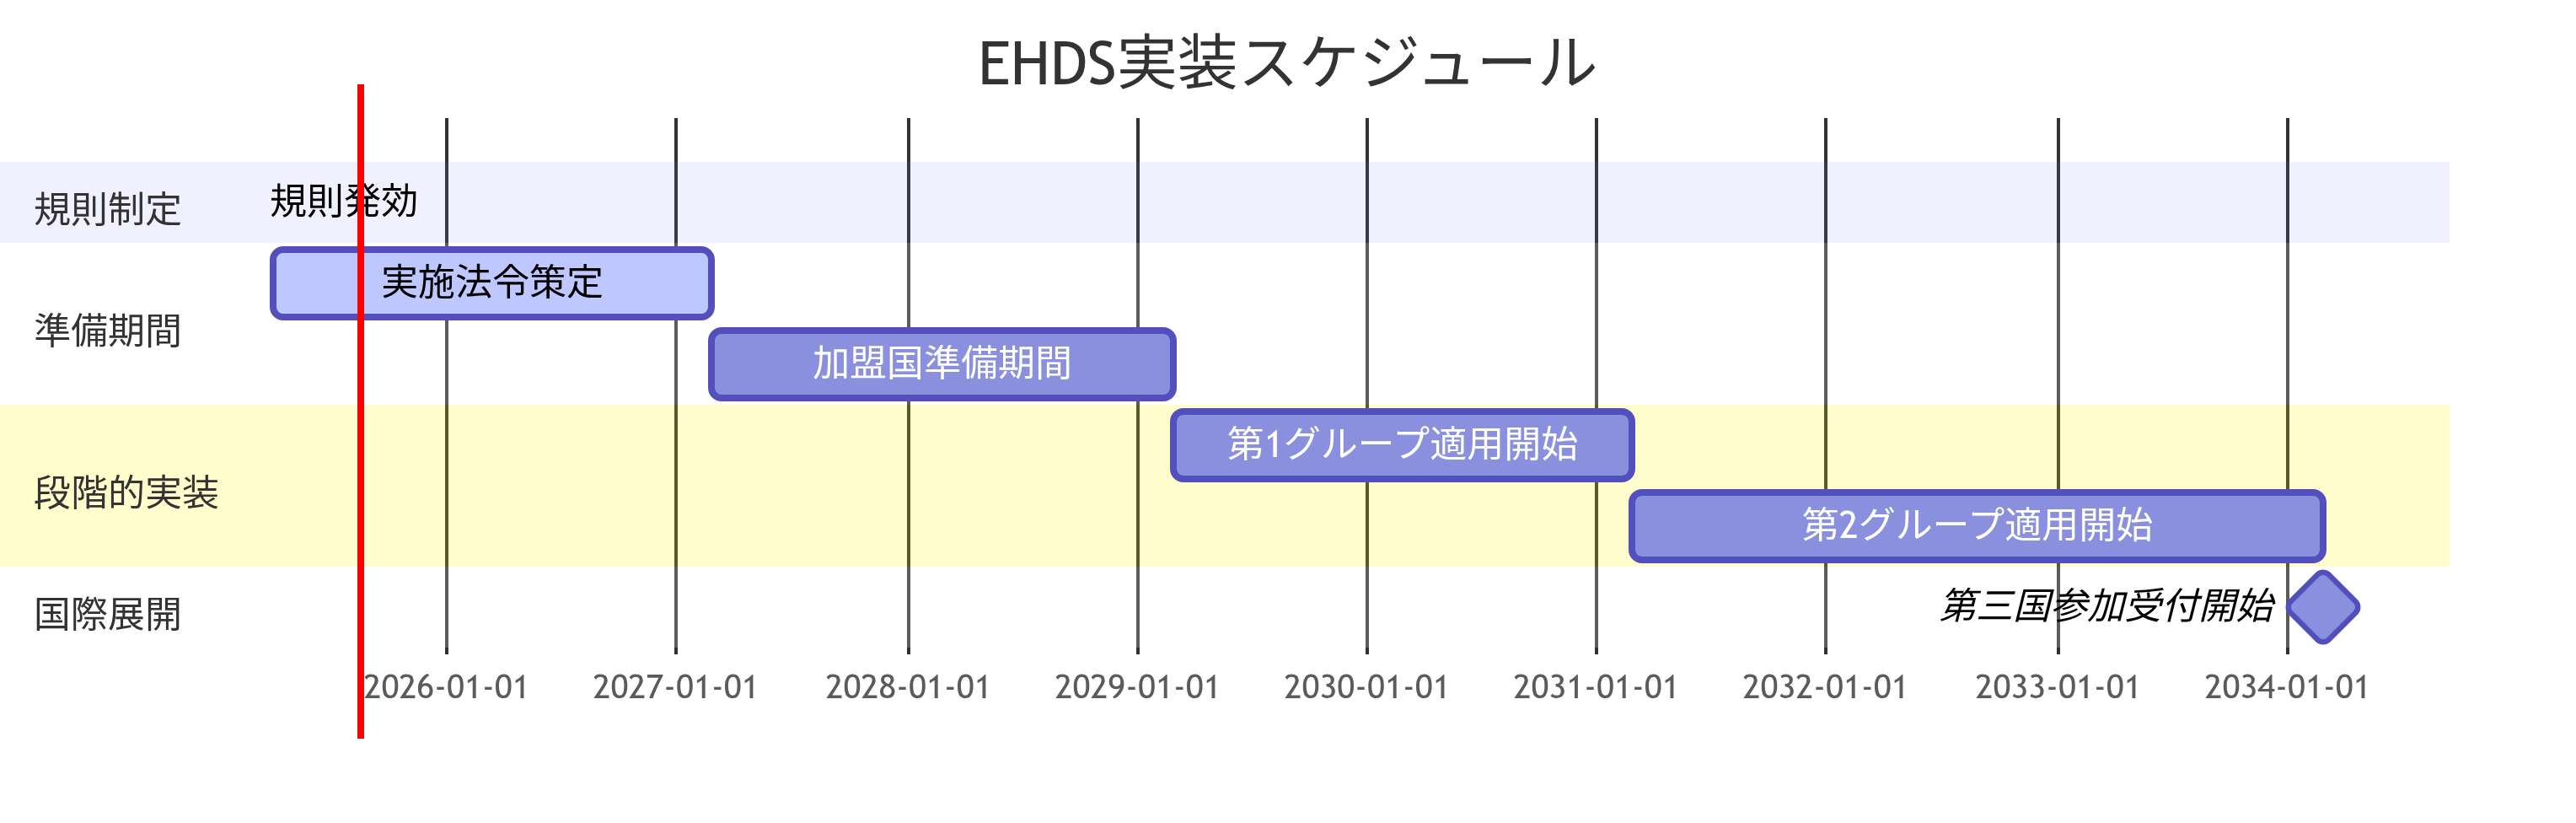
\includegraphics[width=7.96in,height=2.54in]{01-introduction_files/figure-latex/mermaid-figure-1.png}

EHDS実装タイムライン（公式スケジュール）

\begin{tcolorbox}[enhanced jigsaw, toprule=.15mm, bottomtitle=1mm, coltitle=black, left=2mm, opacityback=0, arc=.35mm, colbacktitle=quarto-callout-note-color!10!white, colback=white, opacitybacktitle=0.6, bottomrule=.15mm, rightrule=.15mm, breakable, title=\textcolor{quarto-callout-note-color}{\faInfo}\hspace{0.5em}{Note}, toptitle=1mm, titlerule=0mm, colframe=quarto-callout-note-color-frame, leftrule=.75mm]

\textbf{注記}：このタイムラインは規則で定められた法的期限だが、技術的・組織的複雑性により遅延の可能性も指摘されている。

\end{tcolorbox}

\section{国際的な影響}\label{ux56fdux969bux7684ux306aux5f71ux97ff}

EHDSは、EU域内だけでなく、グローバルな医療データ標準に影響を与える可能性が高い{[}13{]},
{[}15{]}：

\begin{itemize}
\tightlist
\item
  \textbf{標準化の波及効果}：FHIR、HL7などの国際標準の採用促進{[}10{]}
\item
  \textbf{規制のブリュッセル効果}：GDPRと同様の世界的影響
\item
  \textbf{市場アクセス条件}：EU市場参入にはEHDS準拠が必須に{[}1{]}
\item
  \textbf{国際協力の枠組み}：第三国との相互運用性協定{[}15{]}
\end{itemize}

\chapter{規制フレームワーク}\label{ux898fux5236ux30d5ux30ecux30fcux30e0ux30efux30fcux30af}

\section{法的基盤}\label{ux6cd5ux7684ux57faux76e4}

\textbf{事実}：EHDS規則（EU
2025/327）は、既存のEU規制（GDPR、医療機器規則等）を基盤として、医療データ特有の規定を追加した包括的な法的枠組みである。欧州官報（Official
Journal L
76/1）への掲載（2025年3月5日）から20日後の2025年3月26日に発効し、段階的実装が進行中である{[}1{]}。Arnold
\&
Porterの分析によると、この規則は「欧州の医療データエコシステムにおける画期的な転換点」とされている{[}16{]}。

\subsection{主要な規制要素}\label{ux4e3bux8981ux306aux898fux5236ux8981ux7d20}

\begin{longtable}[]{@{}
  >{\raggedright\arraybackslash}p{(\linewidth - 6\tabcolsep) * \real{0.2000}}
  >{\raggedright\arraybackslash}p{(\linewidth - 6\tabcolsep) * \real{0.4000}}
  >{\raggedright\arraybackslash}p{(\linewidth - 6\tabcolsep) * \real{0.2000}}
  >{\raggedright\arraybackslash}p{(\linewidth - 6\tabcolsep) * \real{0.2000}}@{}}
\toprule\noalign{}
\begin{minipage}[b]{\linewidth}\raggedright
規制項目
\end{minipage} & \begin{minipage}[b]{\linewidth}\raggedright
内容
\end{minipage} & \begin{minipage}[b]{\linewidth}\raggedright
日本での対応状況
\end{minipage} & \begin{minipage}[b]{\linewidth}\raggedright
出典
\end{minipage} \\
\midrule\noalign{}
\endhead
\bottomrule\noalign{}
\endlastfoot
データポータビリティ & 患者による自己データの完全なコントロール &
部分的対応 & {[}1{]} \\
越境データ移転 & EU域内での自由なデータ流通 & 未整備 & {[}1{]} \\
二次利用規定 & 研究目的での利用に関する明確なルール & 検討中 &
{[}1{]} \\
セキュリティ要件 & 高度な暗号化と監査証跡の義務化 & 一部対応 & {[}1{]},
{[}17{]} \\
\end{longtable}

\textbf{考察}：日本の現行制度はEHDSの要求水準に達していない領域が多く、特に越境データ移転と二次利用規定の整備が急務である。

\section{データガバナンス体制}\label{ux30c7ux30fcux30bfux30acux30d0ux30caux30f3ux30b9ux4f53ux5236}

\textbf{事実}：EHDSのガバナンスは3層構造で実装される{[}18{]}：

\begin{enumerate}
\def\labelenumi{\arabic{enumi}.}
\tightlist
\item
  \textbf{EU レベル}: 欧州健康データスペース委員会（EHDS Board）-
  2025年6月設立予定
\item
  \textbf{国家レベル}: 各国の健康データ当局 - 2027年3月までに設置義務
\item
  \textbf{地域レベル}: 地域健康データアクセスポイント -
  2029年3月までに運用開始
\end{enumerate}

\subsection{罰則規定}\label{ux7f70ux5247ux898fux5b9a}

\begin{tcolorbox}[enhanced jigsaw, toprule=.15mm, bottomtitle=1mm, coltitle=black, left=2mm, opacityback=0, arc=.35mm, colbacktitle=quarto-callout-warning-color!10!white, colback=white, opacitybacktitle=0.6, bottomrule=.15mm, rightrule=.15mm, breakable, title=\textcolor{quarto-callout-warning-color}{\faExclamationTriangle}\hspace{0.5em}{Warning}, toptitle=1mm, titlerule=0mm, colframe=quarto-callout-warning-color-frame, leftrule=.75mm]

\textbf{重要}：違反時は最大2000万ユーロまたは年間売上高の4\%の制裁金が科される{[}19{]}。

\end{tcolorbox}

\textbf{考察}：この厳格なガバナンス体制と高額な罰則は、データ保護の実効性を担保する仕組みとして機能することが期待される。

\section{患者の権利}\label{ux60a3ux8005ux306eux6a29ux5229}

\subsection{データへのアクセス権}\label{ux30c7ux30fcux30bfux3078ux306eux30a2ux30afux30bbux30b9ux6a29}

患者は以下の権利を有する：

\begin{itemize}
\tightlist
\item
  \textbf{即時アクセス}: 自己の健康データへの無料アクセス
\item
  \textbf{データポータビリティ}: 標準形式でのデータ取得
\item
  \textbf{修正権}: 誤ったデータの訂正要求
\item
  \textbf{削除権}: 特定条件下でのデータ削除（忘れられる権利）
\end{itemize}

\subsection{データ共有のコントロール}\label{ux30c7ux30fcux30bfux5171ux6709ux306eux30b3ux30f3ux30c8ux30edux30fcux30eb}


\includegraphics[width=9.64in,height=2.9in]{02-regulatory-framework_files/figure-latex/mermaid-figure-1.png}

患者データ共有の同意フロー

\section{禁止される利用目的}\label{ux7981ux6b62ux3055ux308cux308bux5229ux7528ux76eeux7684}

EHDSでは、以下の目的での健康データ利用が明確に禁止されている：

\begin{tcolorbox}[enhanced jigsaw, toprule=.15mm, bottomtitle=1mm, coltitle=black, left=2mm, opacityback=0, arc=.35mm, colbacktitle=quarto-callout-important-color!10!white, colback=white, opacitybacktitle=0.6, bottomrule=.15mm, rightrule=.15mm, breakable, title=\textcolor{quarto-callout-important-color}{\faExclamation}\hspace{0.5em}{禁止事項}, toptitle=1mm, titlerule=0mm, colframe=quarto-callout-important-color-frame, leftrule=.75mm]

\begin{itemize}
\tightlist
\item
  保険料の引き上げや保険加入の拒否
\item
  雇用における差別的取り扱い
\item
  マーケティング目的での個人への直接的なアプローチ
\item
  有害な製品・サービスの開発
\end{itemize}

\end{tcolorbox}

\section{各国の実装義務}\label{ux5404ux56fdux306eux5b9fux88c5ux7fa9ux52d9}

\subsection{必須要件（2027年3月まで）}\label{ux5fc5ux9808ux8981ux4ef62027ux5e743ux6708ux307eux3067}

\begin{enumerate}
\def\labelenumi{\arabic{enumi}.}
\tightlist
\item
  \textbf{国家健康データ当局の設置}

  \begin{itemize}
  \tightlist
  \item
    独立性の確保
  \item
    十分な予算と人員の配置
  \item
    技術的専門性の確保
  \end{itemize}
\item
  \textbf{データ品質基準の策定}

  \begin{itemize}
  \tightlist
  \item
    データの完全性
  \item
    正確性の確保
  \item
    相互運用性の保証
  \end{itemize}
\item
  \textbf{セキュアプロセッシング環境の構築}

  \begin{itemize}
  \tightlist
  \item
    暗号化技術の実装
  \item
    アクセス制御の強化
  \item
    監査ログの完備
  \end{itemize}
\end{enumerate}

\subsection{推奨要件（2029年3月まで）}\label{ux63a8ux5968ux8981ux4ef62029ux5e743ux6708ux307eux3067}

\begin{itemize}
\tightlist
\item
  オプトアウトシステムの導入検討
\item
  市民向け啓発プログラムの実施
\item
  医療従事者向け研修の実施
\end{itemize}

\section{第三国との関係}\label{ux7b2cux4e09ux56fdux3068ux306eux95a2ux4fc2}

\textbf{事実}：EHDSは、十分性認定を受けた第三国とのデータ交換を可能にする枠組みを含んでいる{[}15{]}。

\subsection{日本への影響}\label{ux65e5ux672cux3078ux306eux5f71ux97ff}

日本がEU市場で医療関連ビジネスを展開する場合：

\begin{enumerate}
\def\labelenumi{\arabic{enumi}.}
\tightlist
\item
  \textbf{EHDS準拠の必要性}

  \begin{itemize}
  \tightlist
  \item
    技術標準への適合
  \item
    セキュリティ要件の充足
  \item
    ガバナンス体制の整備
  \end{itemize}
\item
  \textbf{相互運用性の確保}

  \begin{itemize}
  \tightlist
  \item
    FHIR標準の採用
  \item
    用語・コード体系の統一
  \item
    API仕様の共通化
  \end{itemize}
\item
  \textbf{認証取得}

  \begin{itemize}
  \tightlist
  \item
    EU認定機関による審査
  \item
    定期的な監査への対応
  \item
    継続的な改善の実施
  \end{itemize}
\end{enumerate}

\part{技術と実装}

\chapter{技術アーキテクチャ}\label{ux6280ux8853ux30a2ux30fcux30adux30c6ux30afux30c1ux30e3}

\section{インフラストラクチャ設計}\label{ux30a4ux30f3ux30d5ux30e9ux30b9ux30c8ux30e9ux30afux30c1ux30e3ux8a2dux8a08}

EHDSの技術基盤は、分散型とフェデレーション型のハイブリッドアーキテクチャを採用している。

\subsection{コア技術コンポーネント}\label{ux30b3ux30a2ux6280ux8853ux30b3ux30f3ux30ddux30fcux30cdux30f3ux30c8}

\subsubsection{MyHealth@EU（一次利用基盤）}\label{myhealtheuux4e00ux6b21ux5229ux7528ux57faux76e4}

\textbf{事実}：MyHealth@EU（旧称eHealth Digital Service
Infrastructure）は、電子処方箋と患者サマリーの越境交換サービスを提供する欧州委員会の基幹インフラである。2025年4月時点で全EU加盟国に開放されており、フェデレーション型アーキテクチャを通じて各国のNational
Contact Point for eHealth（NCPeH）を接続している{[}20{]}。

\textbf{確認された技術要素}：

\begin{longtable}[]{@{}
  >{\raggedright\arraybackslash}p{(\linewidth - 4\tabcolsep) * \real{0.3333}}
  >{\raggedright\arraybackslash}p{(\linewidth - 4\tabcolsep) * \real{0.3333}}
  >{\raggedright\arraybackslash}p{(\linewidth - 4\tabcolsep) * \real{0.3333}}@{}}
\toprule\noalign{}
\begin{minipage}[b]{\linewidth}\raggedright
項目
\end{minipage} & \begin{minipage}[b]{\linewidth}\raggedright
内容
\end{minipage} & \begin{minipage}[b]{\linewidth}\raggedright
出典
\end{minipage} \\
\midrule\noalign{}
\endhead
\bottomrule\noalign{}
\endlastfoot
アーキテクチャ & フェデレーション型（各国のNational Contact Point for
eHealth - NCPeHを接続） & {[}20{]} \\
データ交換プロトコル & eDelivery AS4（2025年Release 3より導入） &
欧州委員会発表（2025年3月） \\
認証基盤 & eIDAS規則に基づく電子認証 & {[}21{]} \\
データ形式 & HL7 FHIR R4（患者サマリー、電子処方箋） & {[}10{]},
{[}11{]} \\
実装期限 &
2029年：患者サマリー・電子処方箋2031年：医療画像・検査結果・退院報告書 &
{[}4{]} \\
\end{longtable}

\begin{tcolorbox}[enhanced jigsaw, toprule=.15mm, bottomtitle=1mm, coltitle=black, left=2mm, opacityback=0, arc=.35mm, colbacktitle=quarto-callout-note-color!10!white, colback=white, opacitybacktitle=0.6, bottomrule=.15mm, rightrule=.15mm, breakable, title=\textcolor{quarto-callout-note-color}{\faInfo}\hspace{0.5em}{Note}, toptitle=1mm, titlerule=0mm, colframe=quarto-callout-note-color-frame, leftrule=.75mm]

\textbf{注記}：具体的な性能要件（応答時間、可用性SLA等）や暗号化仕様の詳細は、公開されている技術文書では確認できていない。実装においては各国の技術要件に従うものと考えられる。

\end{tcolorbox}

\subsubsection{HealthData@EU（二次利用基盤）}\label{healthdataeuux4e8cux6b21ux5229ux7528ux57faux76e4}

\textbf{事実}：HealthData@EU中央プラットフォームRelease 3は、DG
SANTEから初めてオープンソースとして2025年3月26日に公開された。モジュール型アーキテクチャを採用し、各プロジェクトが独立してデプロイ可能な設計となっており、加盟国が再利用可能なビルディングブロックとして活用できる{[}22{]}。2027年の本格運用開始を目指し、現在受け入れ環境で開発版が利用可能である。

\textbf{EHDS規則で定められた二次利用の目的}{[}2{]}：

\begin{itemize}
\tightlist
\item
  研究活動（科学研究、応用研究）
\item
  イノベーション活動（AI開発、医療機器開発等）
\item
  政策立案（公衆衛生、医療システム改善）
\item
  規制活動（医薬品・医療機器の市販後調査等）
\item
  教育活動（医療従事者の訓練）
\end{itemize}

\section{相互運用性フレームワーク}\label{ux76f8ux4e92ux904bux7528ux6027ux30d5ux30ecux30fcux30e0ux30efux30fcux30af}

\subsection{EHDSの技術スタック階層}\label{ehdsux306eux6280ux8853ux30b9ux30bfux30c3ux30afux968eux5c64}

EHDSの相互運用性は、複数の標準規格を階層的に組み合わせて実現されている。

\begin{figure}[H]

{\centering 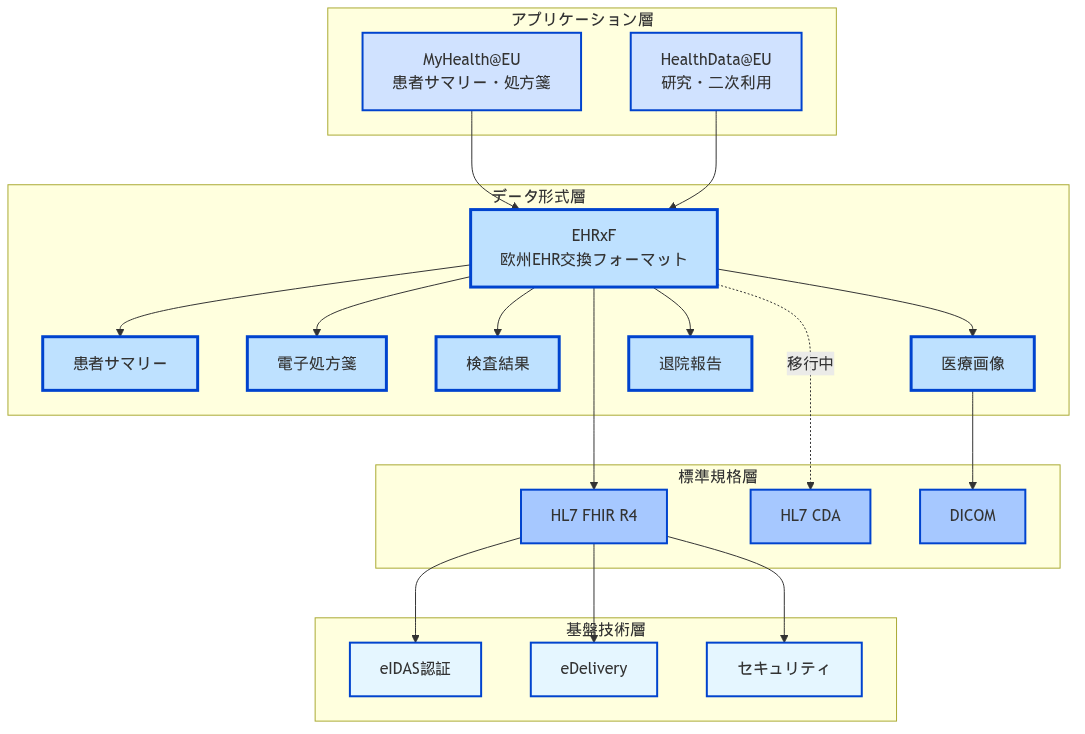
\includegraphics[width=1\linewidth,height=\textheight,keepaspectratio]{images/tech-stack.png}

}

\caption{EHDSの技術スタックとEHRxF/FHIRの位置づけ}

\end{figure}%

\subsection{EHRxFとFHIRの関係}\label{ehrxfux3068fhirux306eux95a2ux4fc2}

\textbf{事実}：欧州電子健康記録交換フォーマット（EHRxF）は、HL7 FHIR
R4を基盤として構築されており、従来のCDA（Clinical Document
Architecture）からFHIRへの移行が進行中である。2025年5月28日、HL7
EuropeはEHDS向けの4つのFHIR実装ガイドのパブリックレビューを開始した{[}10{]}。

\textbf{技術的な位置づけ}：

\begin{longtable}[]{@{}
  >{\raggedright\arraybackslash}p{(\linewidth - 4\tabcolsep) * \real{0.2727}}
  >{\raggedright\arraybackslash}p{(\linewidth - 4\tabcolsep) * \real{0.2727}}
  >{\raggedright\arraybackslash}p{(\linewidth - 4\tabcolsep) * \real{0.4545}}@{}}
\toprule\noalign{}
\begin{minipage}[b]{\linewidth}\raggedright
要素
\end{minipage} & \begin{minipage}[b]{\linewidth}\raggedright
役割
\end{minipage} & \begin{minipage}[b]{\linewidth}\raggedright
実装状況
\end{minipage} \\
\midrule\noalign{}
\endhead
\bottomrule\noalign{}
\endlastfoot
\textbf{EHRxF} & 欧州統一のデータ交換フォーマット仕様 &
6つの優先カテゴリーを定義 \\
\textbf{FHIR} & EHRxFの技術的基盤となる国際標準 & R4バージョンを採用 \\
\textbf{実装ガイド} & 各データカテゴリー別の具体的実装方法 &
順次策定・公開中 \\
\end{longtable}

\subsection{HL7
FHIR標準の採用}\label{hl7-fhirux6a19ux6e96ux306eux63a1ux7528}

\subsubsection{FHIRとは}\label{fhirux3068ux306f}

\textbf{HL7 FHIR（Fast Healthcare Interoperability
Resources）}は、医療情報の電子的な交換のための次世代標準規格である{[}23{]}。RESTful
APIベースのリソース指向アーキテクチャを採用し、現代的なWeb技術（JSON、XML、HTTP）を活用することで、従来の医療情報標準よりも実装が容易になっている。

\textbf{技術的特徴}{[}23{]}：

\begin{itemize}
\tightlist
\item
  \textbf{RESTful設計}: REST成熟度モデルのLevel 2準拠、Level 3拡張可能
\item
  \textbf{データ形式}: JSON、XML、RDFをサポート
\item
  \textbf{リソース構造}: モジュール型の再利用可能コンポーネント
\item
  \textbf{拡張機能}: Extensionメカニズムによる柔軟なカスタマイズ
\end{itemize}

\subsubsection{EHDSにおけるFHIR採用の背景}\label{ehdsux306bux304aux3051ux308bfhirux63a1ux7528ux306eux80ccux666f}

\textbf{事実}：eHealth
Network（eHN）は、検査レポート等のガイドライン実装のためにHL7
FHIR標準を選択した。現在のMyHealth@EUインフラはHL7標準に基づいており、今後はFHIR標準に基づいてサービスを拡張する{[}10{]}。

\textbf{FHIRが選ばれた主な要因}：

\begin{enumerate}
\def\labelenumi{\arabic{enumi}.}
\tightlist
\item
  \textbf{柔軟性と適応性}：リアルタイムの臨床データ交換、エクステンションを通じたカスタマイズが可能
\item
  \textbf{越境医療のサポート}：既存のMyHealth@EUインフラとの互換性
\item
  \textbf{実装ガイドの開発}：HL7
  EuropeがEHDS優先カテゴリー向けの実装ガイドを策定
\end{enumerate}

\begin{tcolorbox}[enhanced jigsaw, toprule=.15mm, bottomtitle=1mm, coltitle=black, left=2mm, opacityback=0, arc=.35mm, colbacktitle=quarto-callout-note-color!10!white, colback=white, opacitybacktitle=0.6, bottomrule=.15mm, rightrule=.15mm, breakable, title=\textcolor{quarto-callout-note-color}{\faInfo}\hspace{0.5em}{Note}, toptitle=1mm, titlerule=0mm, colframe=quarto-callout-note-color-frame, leftrule=.75mm]

\textbf{注記}：EEHRxF（European Electronic Health Record Exchange
Format）は現在CDAからFHIRへの移行が進行中であり、2029年までに完全移行が目指されている。

\end{tcolorbox}

\begin{longtable}[]{@{}
  >{\raggedright\arraybackslash}p{(\linewidth - 4\tabcolsep) * \real{0.3571}}
  >{\raggedright\arraybackslash}p{(\linewidth - 4\tabcolsep) * \real{0.2143}}
  >{\raggedright\arraybackslash}p{(\linewidth - 4\tabcolsep) * \real{0.4286}}@{}}
\toprule\noalign{}
\begin{minipage}[b]{\linewidth}\raggedright
従来標準
\end{minipage} & \begin{minipage}[b]{\linewidth}\raggedright
課題
\end{minipage} & \begin{minipage}[b]{\linewidth}\raggedright
FHIRの利点
\end{minipage} \\
\midrule\noalign{}
\endhead
\bottomrule\noalign{}
\endlastfoot
HL7 v2 & パイプ区切りテキスト、カスタム実装が必要 & RESTful
API、標準的なWeb技術 \\
HL7 v3/CDA & XML文書形式、高い複雑性 &
モジュール型リソース、段階的実装可能 \\
各国独自規格 & 相互運用性の欠如 & 国際標準、拡張機能による柔軟性 \\
\end{longtable}

\textbf{事実}：EHDSは2025年3月の規則施行により、28加盟国間での標準化された健康データ交換を実現するためHL7
FHIR標準を採用。10年間で10.8億ユーロ（一次利用5.4億ユーロ、二次利用5.4億ユーロ）の経済効果が見込まれている{[}2{]}。

\subsubsection{欧州と日本のFHIR実装アプローチ}\label{ux6b27ux5ddeux3068ux65e5ux672cux306efhirux5b9fux88c5ux30a2ux30d7ux30edux30fcux30c1}

\textbf{事実}：FHIRは欧州で規制主導により採用が進む一方、日本では日本医療情報学会（JAMI）NeXEHRS研究会主導でJP
Core（HOTコード、YJコード対応）として独自拡張されている{[}24{]}。

\begin{longtable}[]{@{}
  >{\raggedright\arraybackslash}p{(\linewidth - 4\tabcolsep) * \real{0.1622}}
  >{\raggedright\arraybackslash}p{(\linewidth - 4\tabcolsep) * \real{0.3784}}
  >{\raggedright\arraybackslash}p{(\linewidth - 4\tabcolsep) * \real{0.4595}}@{}}
\toprule\noalign{}
\begin{minipage}[b]{\linewidth}\raggedright
観点
\end{minipage} & \begin{minipage}[b]{\linewidth}\raggedright
欧州（EHDS）
\end{minipage} & \begin{minipage}[b]{\linewidth}\raggedright
日本（JP Core）
\end{minipage} \\
\midrule\noalign{}
\endhead
\bottomrule\noalign{}
\endlastfoot
アプローチ & 規制主導（トップダウン） &
コミュニティ主導（ボトムアップ） \\
標準化範囲 & EU全域統一 & 国内医療制度に特化 \\
コード体系 & SNOMED CT、LOINC、ICD-11 & HOTコード、YJコード、MEDIS \\
実装時期 & 2029年から段階的義務化 & 任意採用、段階的普及 \\
バージョン & R4（安定版）、R5（移行準備） & R4ベース（v1.2.0） \\
プロファイル数 & 優先6カテゴリー & 8薬剤プロファイル+23拡張 \\
\end{longtable}

\subsubsection{FHIRリソースの活用}\label{fhirux30eaux30bdux30fcux30b9ux306eux6d3bux7528}

\begin{tcolorbox}[enhanced jigsaw, toprule=.15mm, bottomtitle=1mm, coltitle=black, left=2mm, opacityback=0, arc=.35mm, colbacktitle=quarto-callout-note-color!10!white, colback=white, opacitybacktitle=0.6, bottomrule=.15mm, rightrule=.15mm, breakable, title=\textcolor{quarto-callout-note-color}{\faInfo}\hspace{0.5em}{Note}, toptitle=1mm, titlerule=0mm, colframe=quarto-callout-note-color-frame, leftrule=.75mm]

\textbf{FHIRリソースについて}：EHDSでは、HL7
FHIR標準に基づいた実装ガイドが策定されている。2025年5月にHL7
EuropeがEHDS向けの4つのFHIR実装ガイドのパブリックレビューを開始した{[}10{]}。実装例については、HL7
International Patient Summary (IPS) Implementation Guide
v1.1.0に準拠した公式サンプルが提供されている{[}25{]}。

\end{tcolorbox}


\includegraphics[width=17.14in,height=3.35in]{03-technical-architecture_files/figure-latex/mermaid-figure-1.png}

EHDS優先カテゴリーとFHIR実装ガイドの関係

各優先カテゴリーに対応したFHIRリソース定義が含まれており、具体的なリソースの必須/オプション要件は各実装ガイドで詳細に定義される。

\subsubsection{FHIR
R4とR5の実装戦略}\label{fhir-r4ux3068r5ux306eux5b9fux88c5ux6226ux7565}

\textbf{事実}：HL7 EuropeはFHIR
R4（2019年の安定版）とR5（最新版）の両方で実装ガイドを開発している。これは組織の技術的成熟度に応じた段階的移行を支援するためである{[}10{]}。

\textbf{バージョン選択の考慮事項}：

\begin{longtable}[]{@{}llll@{}}
\toprule\noalign{}
項目 & FHIR R4 & FHIR R5 & 推奨シナリオ \\
\midrule\noalign{}
\endhead
\bottomrule\noalign{}
\endlastfoot
安定性 & Normative（正規版） & Standard for Trial Use & 本番環境はR4 \\
採用率 & 広く実装済み & 限定的 & 既存システムはR4維持 \\
機能 & コア機能完備 & 拡張機能追加 & 新規開発はR5検討 \\
移行パス & - & R4Bブリッジ版経由 & 段階的移行推奨 \\
\end{longtable}

\textbf{R4Bブリッジ版の役割}： -
R4の安定性を維持しながらR5機能を選択的に利用 -
完全なR5移行前の過渡期ソリューション -
リスクを最小化しながら新機能を段階的に採用

\subsubsection{FHIRプロファイリングの実践}\label{fhirux30d7ux30edux30d5ux30a1ux30a4ux30eaux30f3ux30b0ux306eux5b9fux8df5}

\paragraph{プロファイリングとは何か}\label{ux30d7ux30edux30d5ux30a1ux30a4ux30eaux30f3ux30b0ux3068ux306fux4f55ux304b}

\textbf{初心者向け説明}：
FHIRプロファイリングは、標準的な医療データ形式（FHIRリソース）を、特定の国や医療機関の要件に合わせてカスタマイズする仕組みです。例えるなら、「標準的な申請書フォーマット」を「日本の病院用申請書」に調整するようなものです。

\textbf{プロファイルの基本概念}：

\begin{itemize}
\tightlist
\item
  \textbf{標準FHIRリソース}：世界共通の基本的なデータ構造（例：患者情報の基本形）
\item
  \textbf{プロファイル}：その基本形に対して「この項目は必須」「この項目は使わない」などのルールを追加したもの
\item
  \textbf{相互運用性の維持}：カスタマイズしても、他のシステムとデータ交換できる互換性を保つ
\end{itemize}

\textbf{なぜプロファイリングが必要か}：

\begin{enumerate}
\def\labelenumi{\arabic{enumi}.}
\tightlist
\item
  \textbf{各国の医療制度の違い}：保険番号の形式、診療報酬の仕組みなどが国ごとに異なる
\item
  \textbf{法規制の要件}：個人情報保護法、医療法などの国内法への対応
\item
  \textbf{既存システムとの統合}：各国で既に運用されているシステムとの連携
\end{enumerate}

\paragraph{制約の種類と適用例}\label{ux5236ux7d04ux306eux7a2eux985eux3068ux9069ux7528ux4f8b}

\begin{Shaded}
\begin{Highlighting}[]
\ErrorTok{//} \ErrorTok{例：EHDS患者プロファイル（簡略版）}
\FunctionTok{\{}
  \DataTypeTok{"resourceType"}\FunctionTok{:} \StringTok{"StructureDefinition"}\FunctionTok{,}  \ErrorTok{//} \ErrorTok{これがプロファイル定義であることを示す}
  \DataTypeTok{"id"}\FunctionTok{:} \StringTok{"ehds{-}patient"}\FunctionTok{,}                    \ErrorTok{//} \ErrorTok{このプロファイルのID}
  \DataTypeTok{"url"}\FunctionTok{:} \StringTok{"http://ehds.eu/fhir/StructureDefinition/Patient"}\FunctionTok{,}  \ErrorTok{//} \ErrorTok{一意のURL}
  \DataTypeTok{"type"}\FunctionTok{:} \StringTok{"Patient"}\FunctionTok{,}                       \ErrorTok{//} \ErrorTok{カスタマイズ対象のリソースタイプ}
  \DataTypeTok{"derivation"}\FunctionTok{:} \StringTok{"constraint"}\FunctionTok{,}              \ErrorTok{//} \ErrorTok{制約を追加する形式}
  \DataTypeTok{"differential"}\FunctionTok{:} \FunctionTok{\{}                        \ErrorTok{//} \ErrorTok{標準からの差分を定義}
    \DataTypeTok{"element"}\FunctionTok{:} \OtherTok{[}
      \FunctionTok{\{}
        \DataTypeTok{"id"}\FunctionTok{:} \StringTok{"Patient.identifier"}\FunctionTok{,}
        \DataTypeTok{"min"}\FunctionTok{:} \DecValTok{1}\FunctionTok{,}  \ErrorTok{//} \ErrorTok{識別子を必須化（標準では任意）}
        \DataTypeTok{"max"}\FunctionTok{:} \StringTok{"*"} \ErrorTok{//} \ErrorTok{複数の識別子を許可}
      \FunctionTok{\}}\OtherTok{,}
      \FunctionTok{\{}
        \DataTypeTok{"id"}\FunctionTok{:} \StringTok{"Patient.name"}\FunctionTok{,}
        \DataTypeTok{"min"}\FunctionTok{:} \DecValTok{1}\FunctionTok{,}  \ErrorTok{//} \ErrorTok{氏名を必須化（標準では任意）}
        \DataTypeTok{"max"}\FunctionTok{:} \StringTok{"*"} \ErrorTok{//} \ErrorTok{複数の名前（旧姓など）を許可}
      \FunctionTok{\}}\OtherTok{,}
      \FunctionTok{\{}
        \DataTypeTok{"id"}\FunctionTok{:} \StringTok{"Patient.birthDate"}\FunctionTok{,}
        \DataTypeTok{"min"}\FunctionTok{:} \DecValTok{1}   \ErrorTok{//} \ErrorTok{生年月日を必須化（標準では任意）}
      \FunctionTok{\}}
    \OtherTok{]}
  \FunctionTok{\}}
\FunctionTok{\}}
\end{Highlighting}
\end{Shaded}

\textbf{上記のコードが意味すること}：

\begin{itemize}
\tightlist
\item
  EHDSでは患者データに「識別子」「氏名」「生年月日」が必ず含まれていなければならない
\item
  標準FHIRではこれらは任意項目だが、EHDSプロファイルでは必須に変更
\item
  識別子や氏名は複数持つことができる（例：パスポート番号と保険証番号、旧姓と現在の姓）
\end{itemize}

\textbf{カーディナリティ（出現回数）の読み方}：

\begin{itemize}
\tightlist
\item
  \texttt{0..1}: 任意で1つまで（あってもなくてもよいが、最大1つ）
\item
  \texttt{1..1}: 必ず1つ（省略不可、複数不可）
\item
  \texttt{0..*}: 任意で複数可（なくてもよいし、いくつあってもよい）
\item
  \texttt{1..*}: 必ず1つ以上（最低1つは必須、複数可）
\end{itemize}

\textbf{実際の適用例}：

\begin{itemize}
\tightlist
\item
  \textbf{患者ID}：\texttt{1..*}（最低1つの識別子が必要、複数の識別方法を許可）
\item
  \textbf{アレルギー情報}：\texttt{0..*}（アレルギーがない人もいるため任意、複数記録可）
\item
  \textbf{生年月日}：\texttt{1..1}（必ず1つ、複数の誕生日はありえない）
\end{itemize}

\begin{tcolorbox}[enhanced jigsaw, toprule=.15mm, bottomtitle=1mm, coltitle=black, left=2mm, opacityback=0, arc=.35mm, colbacktitle=quarto-callout-important-color!10!white, colback=white, opacitybacktitle=0.6, bottomrule=.15mm, rightrule=.15mm, breakable, title=\textcolor{quarto-callout-important-color}{\faExclamation}\hspace{0.5em}{Important}, toptitle=1mm, titlerule=0mm, colframe=quarto-callout-important-color-frame, leftrule=.75mm]

\textbf{プロファイル設計の重要なポイント}：
各国でプロファイルを作る際は、「必須項目を増やしすぎない」ことが大切です。必須項目が多すぎると、他の国のシステムとデータ交換ができなくなってしまいます。本当に必要な項目だけを必須にして、その他は任意項目として柔軟に対応できるようにすることが、国際的な相互運用性を実現する鍵となります。

\end{tcolorbox}

\subsection{European EHR Exchange Format
(EEHRxF)}\label{european-ehr-exchange-format-eehrxf}

\textbf{事実}：EEHRxF（European Electronic Health Record Exchange
Format）は、EU全域での健康データを標準的な欧州フォーマットで表示・交換するための仕様である。EHDS規則の一部として、相互運用性を確保するための共通フォーマットを提供する{[}3{]}。

\subsubsection{EEHRxFとEHDSの関係}\label{eehrxfux3068ehdsux306eux95a2ux4fc2}

\textbf{EEHRxFの役割}：

\begin{itemize}
\tightlist
\item
  EHDSの技術的基盤として、健康データの標準フォーマットを定義
\item
  HL7 FHIR R4を基盤とした欧州共通の実装仕様
\item
  各国の異なるEHRシステム間でのデータ交換を可能にする
\end{itemize}

\textbf{EHDSで交換される6つの優先データカテゴリー}{[}4{]}：

EHDSの実装において、以下のデータカテゴリーが段階的に導入される：

\textbf{第1グループ（2029年3月までに実装）}：

\begin{enumerate}
\def\labelenumi{\arabic{enumi}.}
\tightlist
\item
  患者サマリー（Patient Summary）
\item
  電子処方箋（ePrescriptions）\\
\item
  電子調剤記録（eDispensations）
\end{enumerate}

\textbf{第2グループ（2031年3月までに実装）}：

\begin{enumerate}
\def\labelenumi{\arabic{enumi}.}
\setcounter{enumi}{3}
\tightlist
\item
  医療画像・レポート（Medical Images and Reports）
\item
  検査結果（Laboratory Results）
\item
  退院報告書（Discharge Reports）
\end{enumerate}

\begin{tcolorbox}[enhanced jigsaw, toprule=.15mm, bottomtitle=1mm, coltitle=black, left=2mm, opacityback=0, arc=.35mm, colbacktitle=quarto-callout-important-color!10!white, colback=white, opacitybacktitle=0.6, bottomrule=.15mm, rightrule=.15mm, breakable, title=\textcolor{quarto-callout-important-color}{\faExclamation}\hspace{0.5em}{Important}, toptitle=1mm, titlerule=0mm, colframe=quarto-callout-important-color-frame, leftrule=.75mm]

\textbf{重要な区別}：

\begin{itemize}
\tightlist
\item
  \textbf{EHDS}：欧州健康データ空間全体の規制枠組み
\item
  \textbf{EEHRxF}：EHDSで使用される技術的なデータフォーマット仕様
\item
  上記のスケジュールはEHDS全体の実装計画であり、EEHRxFはその技術基盤として機能する
\end{itemize}

\end{tcolorbox}

\subsection{用語・コード体系の標準化}\label{ux7528ux8a9eux30b3ux30fcux30c9ux4f53ux7cfbux306eux6a19ux6e96ux5316}

\textbf{事実}：2022年のTEHDAS Joint
Action調査によると、EU加盟国で最も使用されている標準は、セマンティック相互運用性においてICD-10とSNOMED
CTであり、データ交換においてはHL7
FHIRが最も使用されている。ただし、全体的な状況は不均一であり、将来の規制に完全に準拠する準備ができている加盟国はまだない{[}26{]}。

\begin{tcolorbox}[enhanced jigsaw, toprule=.15mm, bottomtitle=1mm, coltitle=black, left=2mm, opacityback=0, arc=.35mm, colbacktitle=quarto-callout-note-color!10!white, colback=white, opacitybacktitle=0.6, bottomrule=.15mm, rightrule=.15mm, breakable, title=\textcolor{quarto-callout-note-color}{\faInfo}\hspace{0.5em}{Note}, toptitle=1mm, titlerule=0mm, colframe=quarto-callout-note-color-frame, leftrule=.75mm]

\textbf{注記}：EHDS規則では用語体系の標準化が相互運用性の鍵となるが、具体的な技術要件は2027年3月までに採択される実施法令で詳細が定められる予定である。現時点では以下の用語体系が欧州で広く使用されている。

\end{tcolorbox}

\begin{longtable}[]{@{}
  >{\raggedright\arraybackslash}p{(\linewidth - 6\tabcolsep) * \real{0.2439}}
  >{\raggedright\arraybackslash}p{(\linewidth - 6\tabcolsep) * \real{0.1463}}
  >{\raggedright\arraybackslash}p{(\linewidth - 6\tabcolsep) * \real{0.2927}}
  >{\raggedright\arraybackslash}p{(\linewidth - 6\tabcolsep) * \real{0.3171}}@{}}
\toprule\noalign{}
\begin{minipage}[b]{\linewidth}\raggedright
用語体系
\end{minipage} & \begin{minipage}[b]{\linewidth}\raggedright
用途
\end{minipage} & \begin{minipage}[b]{\linewidth}\raggedright
EU採用状況
\end{minipage} & \begin{minipage}[b]{\linewidth}\raggedright
日本での対応
\end{minipage} \\
\midrule\noalign{}
\endhead
\bottomrule\noalign{}
\endlastfoot
SNOMED CT & 臨床用語 & 広く使用（一部加盟国） &
研究段階（日本標準病名マスターとのマッピング研究）{[}27{]} \\
LOINC & 検査項目 & 広く使用 &
JLAC10/JLAC11独自コード体系を使用{[}28{]} \\
ICD-10/ICD-11 & 診断分類 & 21ヵ国で使用 &
ICD-10使用中、ICD-11移行計画中{[}29{]} \\
ATC & 医薬品分類 & 推奨 & KEGGで対応、HOT/YJコード併用{[}30{]} \\
UCUM & 単位 & 標準化進行中 & JP Core FHIRで採用済み{[}24{]} \\
\end{longtable}

\begin{tcolorbox}[enhanced jigsaw, toprule=.15mm, bottomtitle=1mm, coltitle=black, left=2mm, opacityback=0, arc=.35mm, colbacktitle=quarto-callout-warning-color!10!white, colback=white, opacitybacktitle=0.6, bottomrule=.15mm, rightrule=.15mm, breakable, title=\textcolor{quarto-callout-warning-color}{\faExclamationTriangle}\hspace{0.5em}{Warning}, toptitle=1mm, titlerule=0mm, colframe=quarto-callout-warning-color-frame, leftrule=.75mm]

\textbf{専門家による確認推奨}：用語・コード体系の標準化は各国の医療制度と密接に関連する複雑な領域です。実装に際しては、医療情報標準化の専門家や各用語体系の認定専門家によるアドバイスを受けることを強く推奨します。特に、国際標準と国内標準のマッピングや相互運用性の確保には、専門的知識が不可欠です。

\end{tcolorbox}

\subsection{日欧の医療データ基盤アーキテクチャ比較}\label{ux65e5ux6b27ux306eux533bux7642ux30c7ux30fcux30bfux57faux76e4ux30a2ux30fcux30adux30c6ux30afux30c1ux30e3ux6bd4ux8f03}

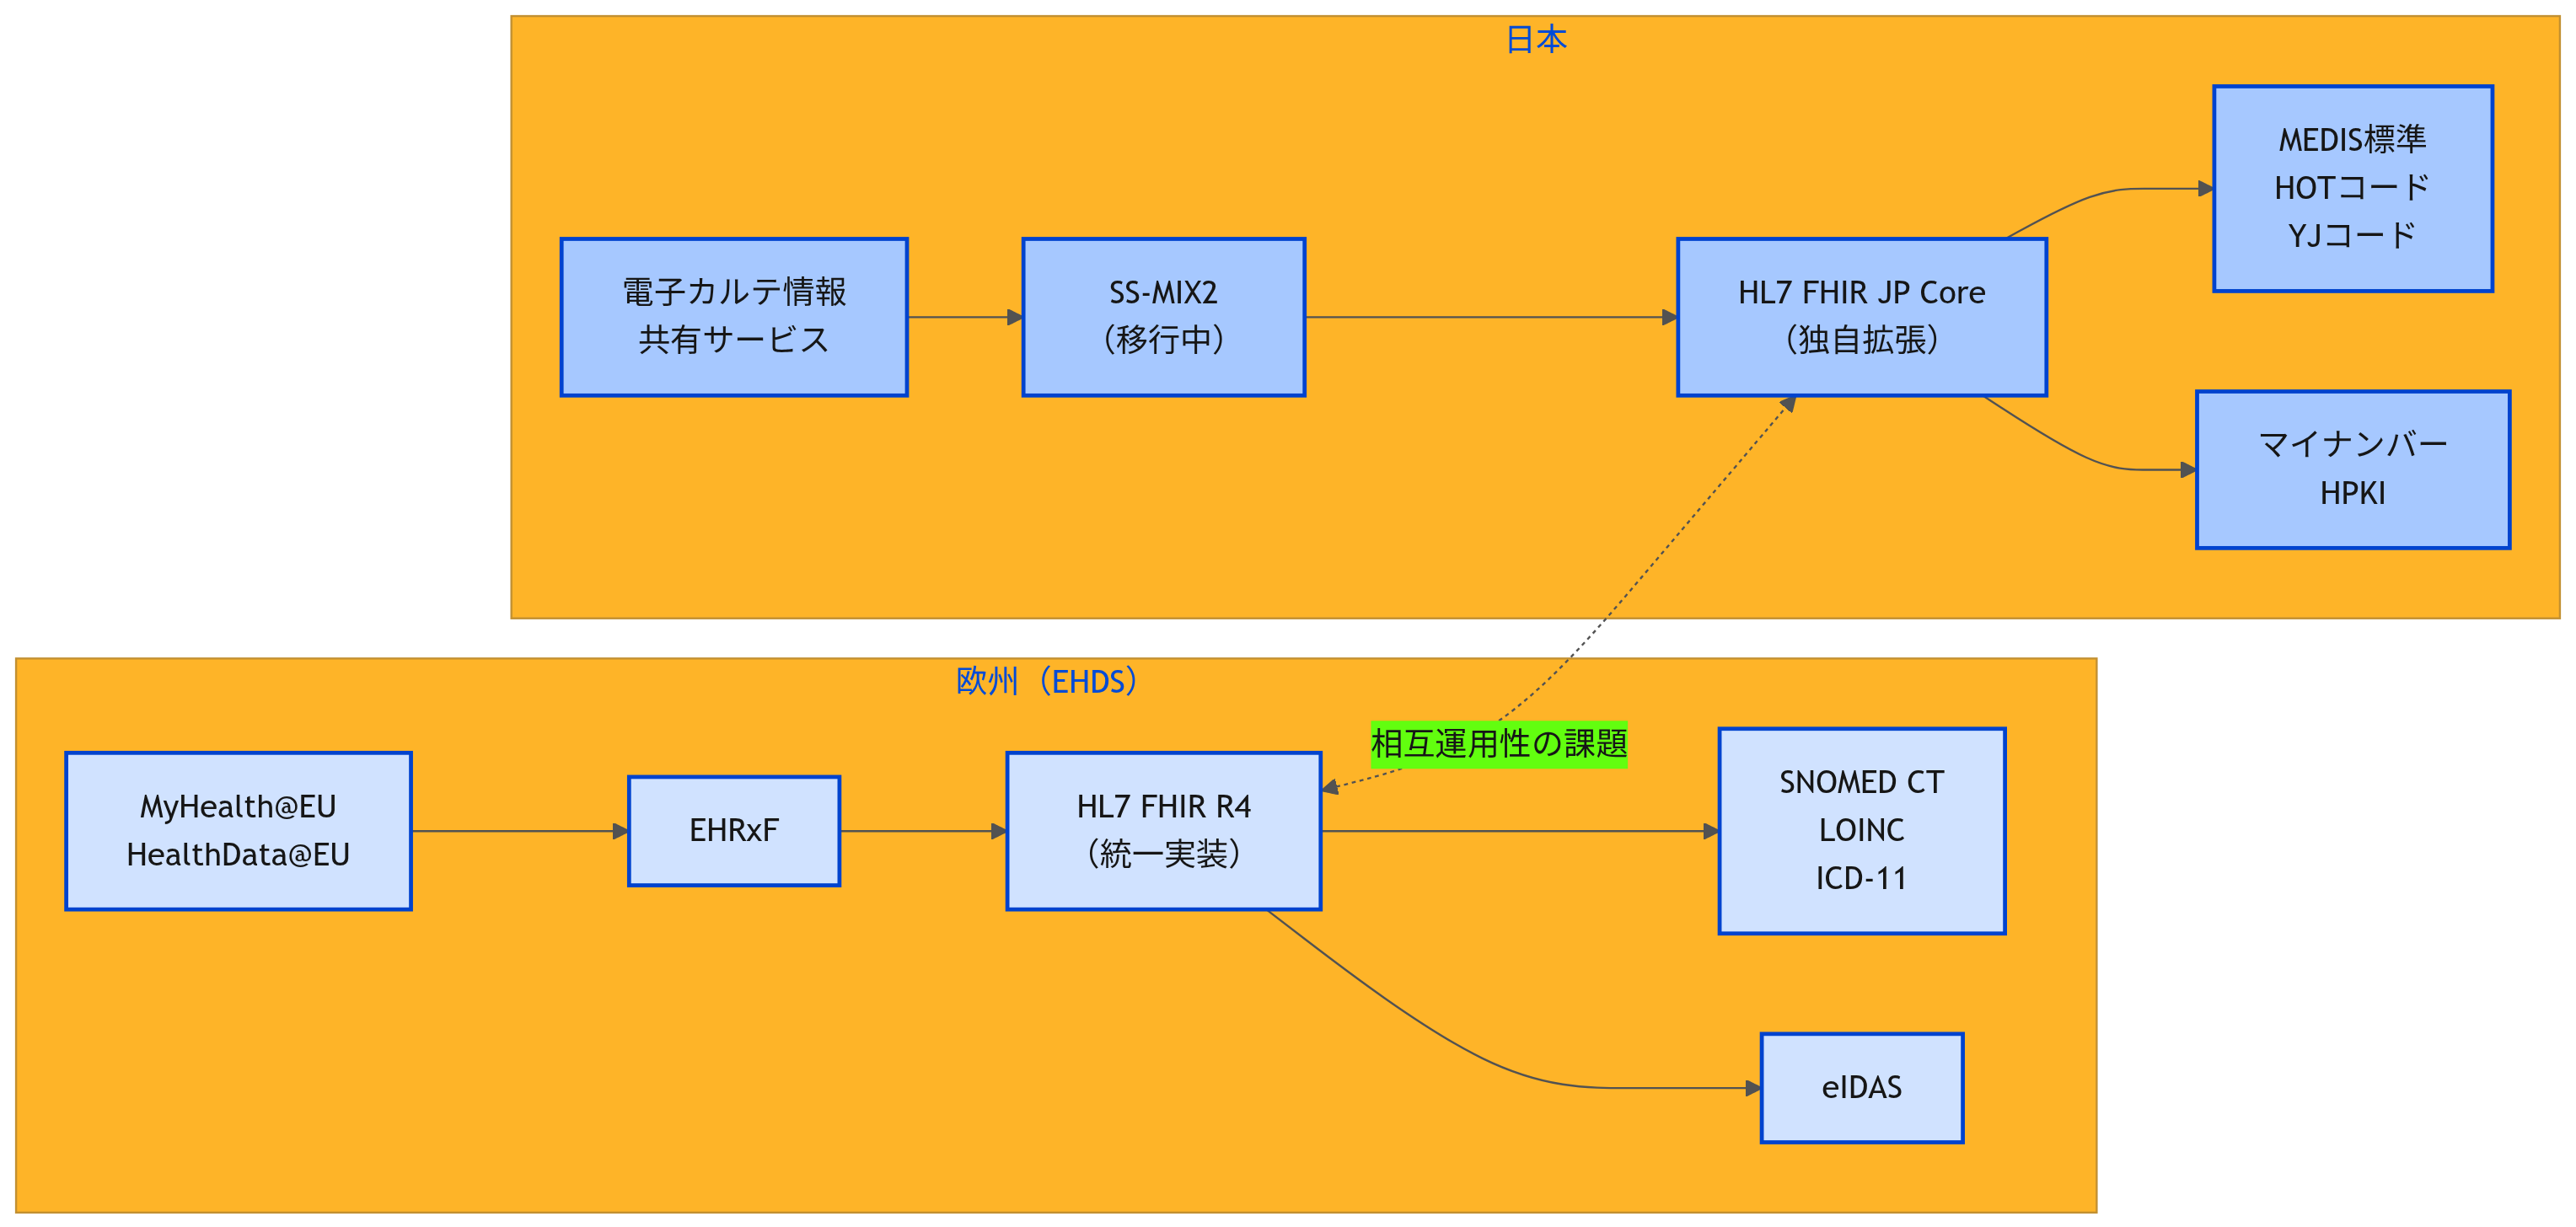
\includegraphics[width=13.36in,height=6.38in]{03-technical-architecture_files/figure-latex/mermaid-figure-7.png}

日本と欧州の医療データ基盤技術スタック比較

\begin{tcolorbox}[enhanced jigsaw, toprule=.15mm, bottomtitle=1mm, coltitle=black, left=2mm, opacityback=0, arc=.35mm, colbacktitle=quarto-callout-note-color!10!white, colback=white, opacitybacktitle=0.6, bottomrule=.15mm, rightrule=.15mm, breakable, title=\textcolor{quarto-callout-note-color}{\faInfo}\hspace{0.5em}{Note}, toptitle=1mm, titlerule=0mm, colframe=quarto-callout-note-color-frame, leftrule=.75mm]

\textbf{技術的相違点}：

\begin{itemize}
\tightlist
\item
  \textbf{データフォーマット}：欧州はEHRxFで統一、日本はSS-MIX2からFHIRへ移行中
\item
  \textbf{FHIR実装}：欧州は統一実装、日本はJP Core独自拡張
\item
  \textbf{用語体系}：欧州は国際標準採用、日本は国内標準を維持
\item
  \textbf{認証基盤}：欧州はeIDAS、日本はマイナンバー/HPKI
\end{itemize}

\end{tcolorbox}

\subsection{日欧相互運用性の技術的課題と解決アプローチ}\label{ux65e5ux6b27ux76f8ux4e92ux904bux7528ux6027ux306eux6280ux8853ux7684ux8ab2ux984cux3068ux89e3ux6c7aux30a2ux30d7ux30edux30fcux30c1}

\textbf{事実}：日本と欧州のFHIR実装の違いは、主に用語体系（日本：HOT/YJコード、欧州：SNOMED
CT/LOINC）とガバナンスモデル（日本：ボトムアップ、欧州：トップダウン）に起因する{[}2{]},
{[}24{]}。2024年の研究では、日本のJP
Coreは8つの薬剤関連プロファイルと23の拡張を含み、HOTコードやYJコードなどの日本独自の用語体系を採用しているため、国際標準との相互運用性に課題があることが指摘されている{[}31{]}。

\begin{tcolorbox}[enhanced jigsaw, toprule=.15mm, bottomtitle=1mm, coltitle=black, left=2mm, opacityback=0, arc=.35mm, colbacktitle=quarto-callout-warning-color!10!white, colback=white, opacitybacktitle=0.6, bottomrule=.15mm, rightrule=.15mm, breakable, title=\textcolor{quarto-callout-warning-color}{\faExclamationTriangle}\hspace{0.5em}{Warning}, toptitle=1mm, titlerule=0mm, colframe=quarto-callout-warning-color-frame, leftrule=.75mm]

\textbf{相互運用性への影響度}：
日欧のFHIR実装の違いは「多少の亜種」ではなく、\textbf{実質的な相互運用性の障壁}となっています。主な影響：

\begin{enumerate}
\def\labelenumi{\arabic{enumi}.}
\tightlist
\item
  \textbf{用語マッピングの複雑性}：HOTコード（約17,000品目）からATC分類への変換には、1対多の対応関係があり自動変換が困難
\item
  \textbf{データ交換の制約}：処方箋の越境交換では、用法用量の表現方法の違いにより再入力が必要
\item
  \textbf{実装コスト}：変換ゲートウェイの開発・運用に年間数千万円規模の投資が必要と推定
\end{enumerate}

ただし、これは克服不可能な問題ではなく、段階的なアプローチ（IPS準拠、用語マッピングテーブルの構築、変換APIの開発）により解決可能です{[}31{]}。

\end{tcolorbox}

\subsubsection{主要な相互運用性の課題}\label{ux4e3bux8981ux306aux76f8ux4e92ux904bux7528ux6027ux306eux8ab2ux984c}

\begin{longtable}[]{@{}
  >{\raggedright\arraybackslash}p{(\linewidth - 6\tabcolsep) * \real{0.2174}}
  >{\raggedright\arraybackslash}p{(\linewidth - 6\tabcolsep) * \real{0.2609}}
  >{\raggedright\arraybackslash}p{(\linewidth - 6\tabcolsep) * \real{0.1739}}
  >{\raggedright\arraybackslash}p{(\linewidth - 6\tabcolsep) * \real{0.3478}}@{}}
\toprule\noalign{}
\begin{minipage}[b]{\linewidth}\raggedright
課題領域
\end{minipage} & \begin{minipage}[b]{\linewidth}\raggedright
具体的問題
\end{minipage} & \begin{minipage}[b]{\linewidth}\raggedright
影響度
\end{minipage} & \begin{minipage}[b]{\linewidth}\raggedright
解決アプローチ
\end{minipage} \\
\midrule\noalign{}
\endhead
\bottomrule\noalign{}
\endlastfoot
\textbf{用語マッピング} & HOT⇔ATC、MEDIS⇔SNOMED CT & 高 &
変換テーブル構築、AI支援マッピング \\
\textbf{プロファイル差異} & 必須要素の相違、拡張機能の非互換 & 中 &
共通コアプロファイル策定 \\
\textbf{識別子体系} & マイナンバー⇔eIDAS & 高 &
フェデレーション型ID連携 \\
\textbf{データモデル} & SS-MIX2⇔FHIR移行状況の差 & 中 &
段階的移行、変換ゲートウェイ \\
\end{longtable}

\subsubsection{技術的解決策}\label{ux6280ux8853ux7684ux89e3ux6c7aux7b56}

日欧間の相互運用性を実現するため、以下の複数のアプローチが考えられる：

\subsubsection{アプローチ1: ゲートウェイ方式（Federated
Gateway）}\label{ux30a2ux30d7ux30edux30fcux30c11-ux30b2ux30fcux30c8ux30a6ux30a7ux30a4ux65b9ux5f0ffederated-gateway}

\paragraph{用語マッピングサービス}\label{ux7528ux8a9eux30deux30c3ux30d4ux30f3ux30b0ux30b5ux30fcux30d3ux30b9}

\textbf{技術的アーキテクチャ}{[}31{]}：

用語マッピングサービスは、以下の3つの主要な変換機能を提供する：

\begin{itemize}
\tightlist
\item
  \textbf{薬剤コード変換}：HOTコードからATCコードへのセマンティックマッピング
\item
  \textbf{薬価コード変換}：YJコードからRxNormへの直接マッピング
\item
  \textbf{病名変換}：日本標準病名からSNOMED CTへのハイブリッドマッピング
\end{itemize}

\begin{tcolorbox}[enhanced jigsaw, toprule=.15mm, bottomtitle=1mm, coltitle=black, left=2mm, opacityback=0, arc=.35mm, colbacktitle=quarto-callout-note-color!10!white, colback=white, opacitybacktitle=0.6, bottomrule=.15mm, rightrule=.15mm, breakable, title=\textcolor{quarto-callout-note-color}{\faInfo}\hspace{0.5em}{Note}, toptitle=1mm, titlerule=0mm, colframe=quarto-callout-note-color-frame, leftrule=.75mm]

\textbf{マッピングの課題}：日本のJP
Core研究では、HOTコードやYJコードなどの日本独自用語体系から国際標準への変換において、一対多の対応関係や概念の不一致により完全自動化が困難であることが報告されている{[}31{]}。実用化には専門家による検証と段階的なマッピングテーブルの構築が必要である。

\end{tcolorbox}

\textbf{技術的仕組みの詳細}：

用語マッピングサービスは、日本の医療用語体系（HOTコード、YJコード等）と欧州の国際標準（ATC、SNOMED
CT等）を相互変換する核となる技術である{[}31{]}。

\textbf{マッピング処理の流れ}：

\begin{enumerate}
\def\labelenumi{\arabic{enumi}.}
\tightlist
\item
  \textbf{入力データの解析}：日本のFHIRリソースからHOTコード等を抽出
\item
  \textbf{セマンティック変換}：機械学習とルールベースのハイブリッド手法でATCコードに変換
\item
  \textbf{品質評価}：変換結果の適切性を複数の手法で検証
\item
  \textbf{専門家レビュー}：自動変換が困難な場合は専門家による確認
\item
  \textbf{FHIR出力}：欧州標準準拠のFHIRリソースとして出力
\end{enumerate}

\textbf{コア技術要素}：

\begin{itemize}
\tightlist
\item
  \textbf{自然言語処理（NLP）}：薬剤名の意味的類似性を計算
\item
  \textbf{オントロジーマッピング}：概念体系間の関係性を定義
\item
  \textbf{機械学習}：過去のマッピング履歴から最適解を学習
\item
  \textbf{ルールエンジン}：専門家知識をルール化して適用
\end{itemize}

\subsubsection{アプローチ2: 共通プロファイル方式（Common Profile
Layer）}\label{ux30a2ux30d7ux30edux30fcux30c12-ux5171ux901aux30d7ux30edux30d5ux30a1ux30a4ux30ebux65b9ux5f0fcommon-profile-layer}

\begin{tcolorbox}[enhanced jigsaw, toprule=.15mm, bottomtitle=1mm, coltitle=black, left=2mm, opacityback=0, arc=.35mm, colbacktitle=quarto-callout-note-color!10!white, colback=white, opacitybacktitle=0.6, bottomrule=.15mm, rightrule=.15mm, breakable, title=\textcolor{quarto-callout-note-color}{\faInfo}\hspace{0.5em}{Note}, toptitle=1mm, titlerule=0mm, colframe=quarto-callout-note-color-frame, leftrule=.75mm]

\textbf{IPSとは}：International Patient
Summary（国際患者サマリー）は、計画外の国境を越えた医療において必要な最小限かつ必須の健康情報を含むHL7
FHIR文書である。ISO 27269およびEN
17269で規定され、アレルギー、服薬歴、既往歴を必須項目とし、専門分野に依存しない汎用的なデータセットとして設計されている{[}32{]}。

\end{tcolorbox}

\textbf{IPS共通レイヤーのアプローチ}：

\begin{itemize}
\tightlist
\item
  \textbf{基盤技術}：HL7 FHIR R4ベースのIPS実装ガイド（STU 1.1.0）を活用
\item
  \textbf{共通要素の抽出}：

  \begin{itemize}
  \tightlist
  \item
    必須項目：アレルギー・不耐性、服薬歴、既往歴
  \item
    推奨項目：免疫歴、医療機器、診断画像結果
  \item
    任意項目：バイタルサイン、検査結果、治療計画
  \end{itemize}
\item
  \textbf{地域拡張の管理}：IPS拡張メカニズムで各国特有項目に対応
\item
  \textbf{変換プロセス}：

  \begin{enumerate}
  \def\labelenumi{\arabic{enumi}.}
  \tightlist
  \item
    各国プロファイル → IPS共通形式への変換
  \item
    IPS共通形式 → 宛先国プロファイルへの変換
  \item
    用語マッピング（SNOMED CT、LOINC等の国際標準経由）
  \end{enumerate}
\end{itemize}

\textbf{IPSベースの共通形式例}：

IPS共通プロファイルでは、患者の最重要な医療情報を構造化されたFHIR
Bundle形式で表現する：

\begin{itemize}
\tightlist
\item
  \textbf{Bundle}: 複数のFHIRリソースをまとめて送信するためのコンテナ
\item
  \textbf{Composition}: 文書全体の構造と目次を定義するリソース
\item
  \textbf{必須セクション}: アレルギー・服薬歴・既往歴の3つが国際的に必須
\item
  \textbf{任意セクション}:
  バイタルサイン・検査結果・医療機器等を追加可能
\end{itemize}

この共通形式により、日本のJP Core FHIRから欧州のEU Base
FHIRへの変換が標準化される。

\textbf{利点}：

\begin{itemize}
\tightlist
\item
  標準化された共通インターフェース、維持コストの削減
\item
  既存の国際標準に準拠、グローバルな相互運用性
\item
  段階的実装が可能（必須項目から開始）
\end{itemize}

\textbf{欠点}：

\begin{itemize}
\tightlist
\item
  各地域の特殊要件への対応が制限される
\item
  既存システムの大幅な改修が必要な場合がある
\item
  IPSの必須項目が各国で未実装の場合、データ欠損が発生
\end{itemize}

\subsubsection{アプローチ3: 分散型標準化方式（Distributed
Standardization）}\label{ux30a2ux30d7ux30edux30fcux30c13-ux5206ux6563ux578bux6a19ux6e96ux5316ux65b9ux5f0fdistributed-standardization}

\textbf{アーキテクチャの概要}：

単一障害点を排除し、各国が対等なノードとして、標準化されたプロトコルで直接接続する分散アーキテクチャである。

\textbf{主要コンポーネント}：

\begin{itemize}
\tightlist
\item
  \textbf{各国ノード}：自国のデータを保持し、標準化APIを提供
\item
  \textbf{共通標準プロトコル}：IPS + FHIR R5による統一された交換仕様
\item
  \textbf{P2Pネットワーク}：各国が必要に応じて直接接続
\end{itemize}

\textbf{データ交換の流れ}：

\begin{enumerate}
\def\labelenumi{\arabic{enumi}.}
\tightlist
\item
  要求元が対象国に直接アクセス申請
\item
  対象国が自国の規制に基づき承認
\item
  標準化されたAPIで直接データ交換
\item
  各国がアクセスログを分散管理
\end{enumerate}

\textbf{利点}：

\begin{itemize}
\tightlist
\item
  単一障害点の完全排除
\item
  無限のスケーラビリティ
\item
  各国のデータ主権の完全保護
\item
  運用コストの分散化
\end{itemize}

\textbf{欠点}：

\begin{itemize}
\tightlist
\item
  初期の標準化調整が複雑
\item
  各国での実装品質のばらつき
\item
  ネットワーク効果が出るまで時間が必要
\end{itemize}

\subsubsection{推奨実装戦略}\label{ux63a8ux5968ux5b9fux88c5ux6226ux7565}

現実的な実装戦略として、3つの相互運用性アプローチから適切な組み合わせを選択することを推奨する：

\begin{longtable}[]{@{}
  >{\raggedright\arraybackslash}p{(\linewidth - 6\tabcolsep) * \real{0.2609}}
  >{\raggedright\arraybackslash}p{(\linewidth - 6\tabcolsep) * \real{0.3043}}
  >{\raggedright\arraybackslash}p{(\linewidth - 6\tabcolsep) * \real{0.2174}}
  >{\raggedright\arraybackslash}p{(\linewidth - 6\tabcolsep) * \real{0.2174}}@{}}
\toprule\noalign{}
\begin{minipage}[b]{\linewidth}\raggedright
アプローチ
\end{minipage} & \begin{minipage}[b]{\linewidth}\raggedright
適用シナリオ
\end{minipage} & \begin{minipage}[b]{\linewidth}\raggedright
主な利点
\end{minipage} & \begin{minipage}[b]{\linewidth}\raggedright
主な課題
\end{minipage} \\
\midrule\noalign{}
\endhead
\bottomrule\noalign{}
\endlastfoot
\textbf{ゲートウェイ方式} & 短期PoC、限定的な接続 &
実装が容易、既存システム影響小 & 運用コスト、拡張性の限界 \\
\textbf{共通プロファイル方式} & 標準化重視、段階的移行 &
国際標準準拠、維持コスト低 & システム改修、機能制約 \\
\textbf{分散型標準化方式} & 長期的な完全相互運用 &
SPOF排除、無限の拡張性 & 初期調整の複雑性 \\
\end{longtable}

\textbf{段階的実装の推奨}：

\begin{enumerate}
\def\labelenumi{\arabic{enumi}.}
\tightlist
\item
  \textbf{短期（2025-2027）}：ゲートウェイ方式でPoC実装
\item
  \textbf{中期（2027-2030）}：共通プロファイル方式への移行
\item
  \textbf{長期（2030年以降）}：分散型標準化方式による完全相互運用
\end{enumerate}

\subsubsection{短期実装例：ゲートウェイ方式アーキテクチャ}\label{ux77edux671fux5b9fux88c5ux4f8bux30b2ux30fcux30c8ux30a6ux30a7ux30a4ux65b9ux5f0fux30a2ux30fcux30adux30c6ux30afux30c1ux30e3}

短期フェーズで実装するゲートウェイ方式の具体的なアーキテクチャを以下に示す：

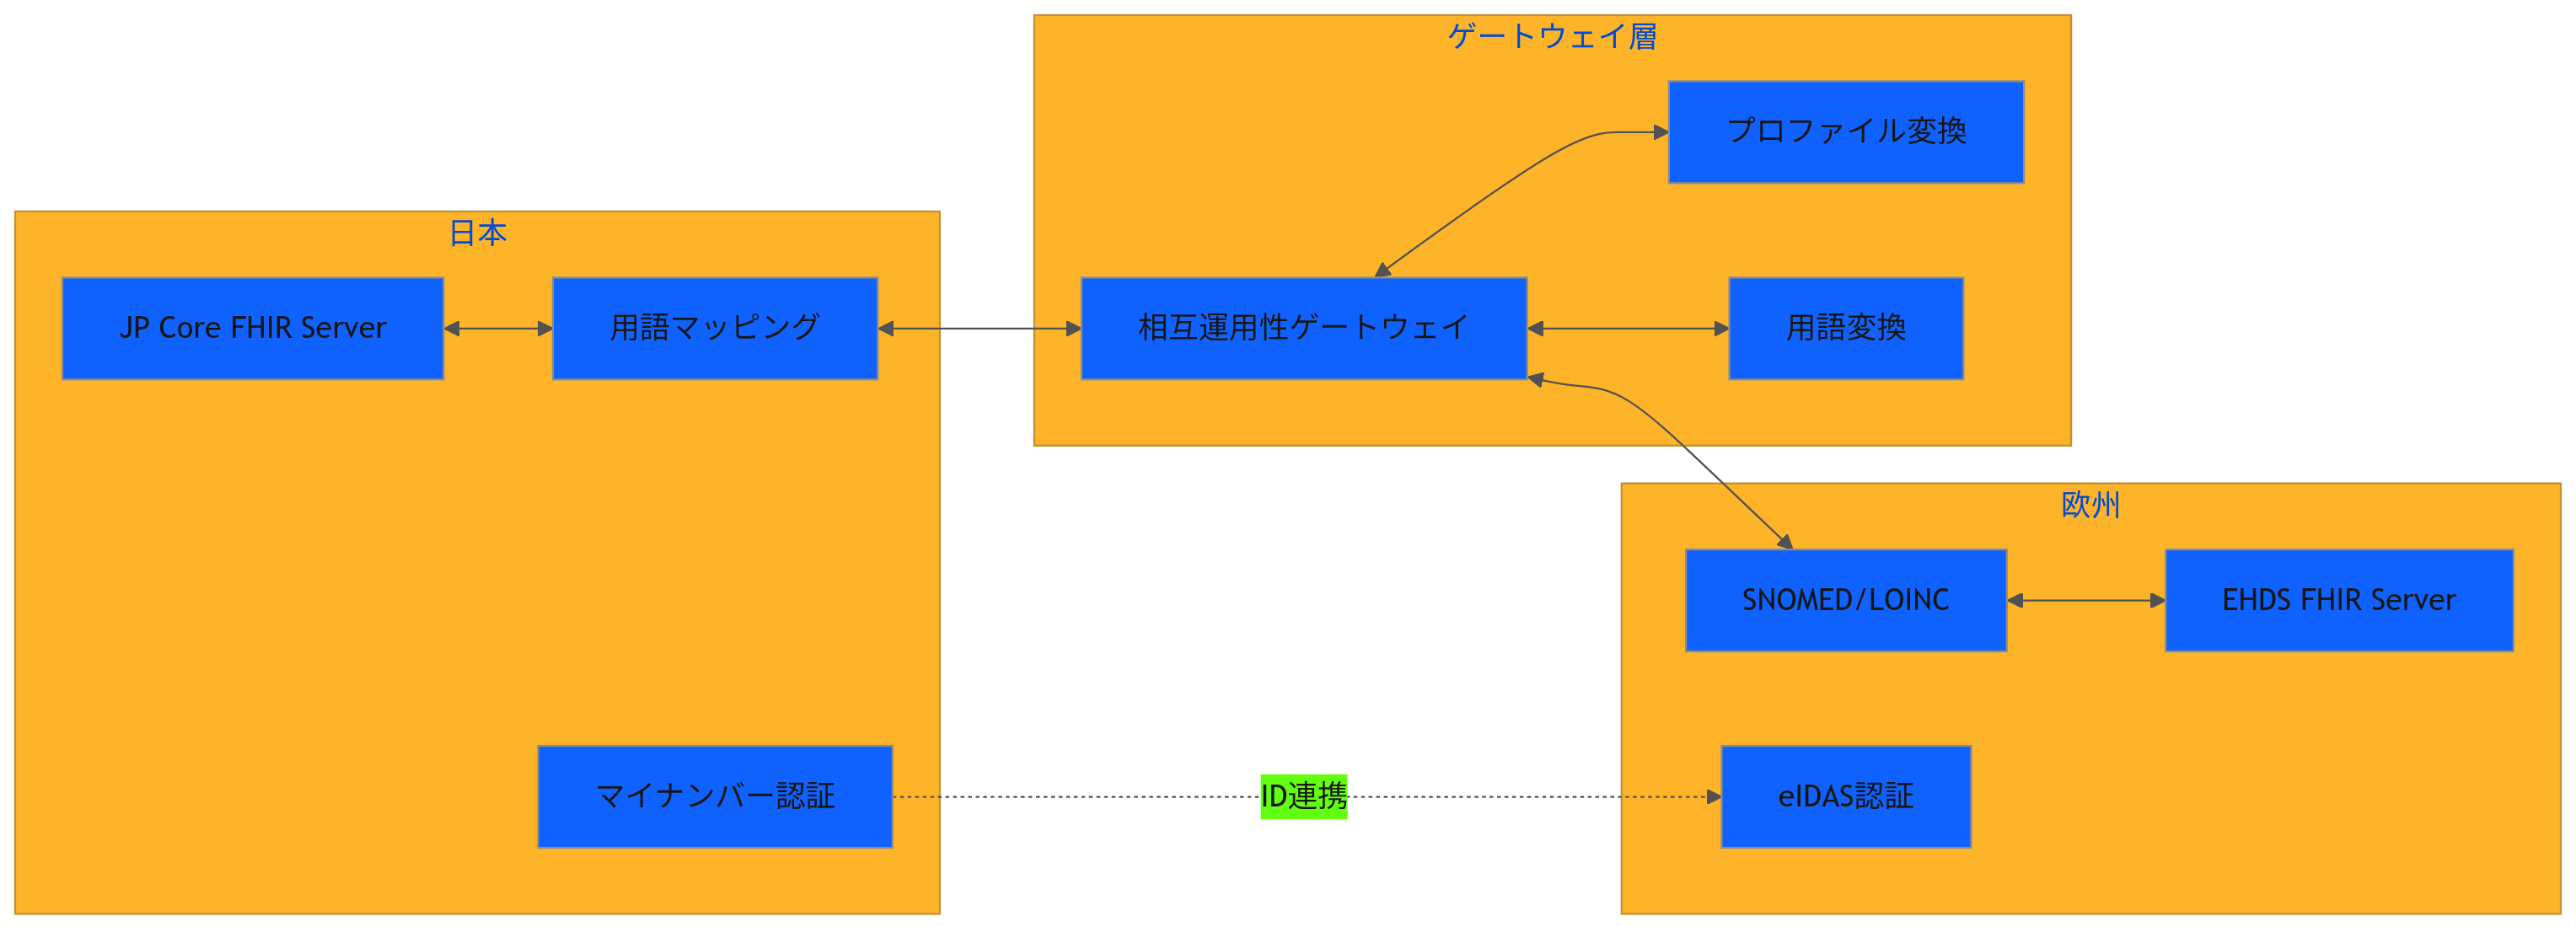
\includegraphics[width=14.21in,height=5.13in]{03-technical-architecture_files/figure-latex/mermaid-figure-6.png}

日欧間相互運用性ゲートウェイアーキテクチャ

\textbf{ゲートウェイによる医療データ相互運用の仕組み}：

このアーキテクチャは、日本と欧州の異なる医療データ標準間で、患者情報を安全に変換・交換するための仕組みである。

\textbf{実用的なデータ交換シナリオ}：

\textbf{ケース1：緊急医療での患者情報照会} -
日本人旅行者がドイツで救急搬送された場合 -
ドイツの医師が患者の服薬歴・アレルギー情報を照会 -
ゲートウェイが日本の電子カルテデータを欧州標準に変換して提供

\textbf{ケース2：国際共同研究でのデータ活用} -
日欧共同での医薬品副作用研究 -
日本の臨床データを欧州の研究プラットフォームで解析 -
用語・単位・プロファイルを統一形式に変換

\textbf{主要な変換処理}：

\begin{enumerate}
\def\labelenumi{\arabic{enumi}.}
\item
  \textbf{用語変換の具体例}：

  \begin{itemize}
  \tightlist
  \item
    薬剤：ロキソニン（HOT9534567）→ Loxoprofen（ATC: M01AE01）
  \item
    診断：本態性高血圧症（日本標準病名）→ Essential hypertension（SNOMED
    CT: 59621000）
  \item
    検査：血糖値（JLAC10: 3F015）→ Glucose（LOINC: 2345-7）
  \end{itemize}
\item
  \textbf{プロファイル変換の具体例}：

  \begin{itemize}
  \tightlist
  \item
    JP Core：患者ID（マイナンバー）→ EHDS：患者ID（eIDAS識別子）
  \item
    JP Core：用法用量（日本語テキスト）→ EHDS：構造化された投与指示
  \item
    JP Core：検査結果単位（mg/dl）→ EHDS：SI単位（mmol/L）
  \end{itemize}
\item
  \textbf{データ構造変換の具体例}：

\begin{Shaded}
\begin{Highlighting}[]
\ErrorTok{//} \ErrorTok{変換前（JP} \ErrorTok{Core）}
\FunctionTok{\{}
  \DataTypeTok{"resourceType"}\FunctionTok{:} \StringTok{"MedicationRequest"}\FunctionTok{,}
  \DataTypeTok{"medicationCodeableConcept"}\FunctionTok{:} \FunctionTok{\{}
    \DataTypeTok{"coding"}\FunctionTok{:} \OtherTok{[}\FunctionTok{\{}\DataTypeTok{"system"}\FunctionTok{:} \StringTok{"urn:oid:1.2.392.100495.20.2.74"}\FunctionTok{,} \DataTypeTok{"code"}\FunctionTok{:} \StringTok{"HOT9534567"}\FunctionTok{\}}\OtherTok{]}
  \FunctionTok{\}}
\FunctionTok{\}}

\ErrorTok{//} \ErrorTok{変換後（EHDS準拠）}
\FunctionTok{\{}
  \DataTypeTok{"resourceType"}\FunctionTok{:} \StringTok{"MedicationRequest"}\FunctionTok{,} 
  \DataTypeTok{"medicationCodeableConcept"}\FunctionTok{:} \FunctionTok{\{}
    \DataTypeTok{"coding"}\FunctionTok{:} \OtherTok{[}\FunctionTok{\{}\DataTypeTok{"system"}\FunctionTok{:} \StringTok{"http://www.whocc.no/atc"}\FunctionTok{,} \DataTypeTok{"code"}\FunctionTok{:} \StringTok{"M01AE01"}\FunctionTok{\}}\OtherTok{]}
  \FunctionTok{\}}
\FunctionTok{\}}
\end{Highlighting}
\end{Shaded}
\end{enumerate}

\textbf{変換品質の保証}：

\begin{itemize}
\tightlist
\item
  \textbf{医師による確認}：自動変換困難な用語は専門医が検証
\item
  \textbf{変換履歴の記録}：どの日本語用語がどの国際標準に変換されたかを記録
\item
  \textbf{信頼度スコア}：各変換結果に95\%、85\%等の信頼度を付与
\item
  \textbf{エラーハンドリング}：変換不可能な項目は「情報不足」として明示
\end{itemize}

\subsubsection{中期実装例：共通プロファイル方式（IPS）アーキテクチャ}\label{ux4e2dux671fux5b9fux88c5ux4f8bux5171ux901aux30d7ux30edux30d5ux30a1ux30a4ux30ebux65b9ux5f0fipsux30a2ux30fcux30adux30c6ux30afux30c1ux30e3}

中期フェーズでは、International Patient
Summary（IPS）を共通仲介層として活用する標準化アプローチを実装する：

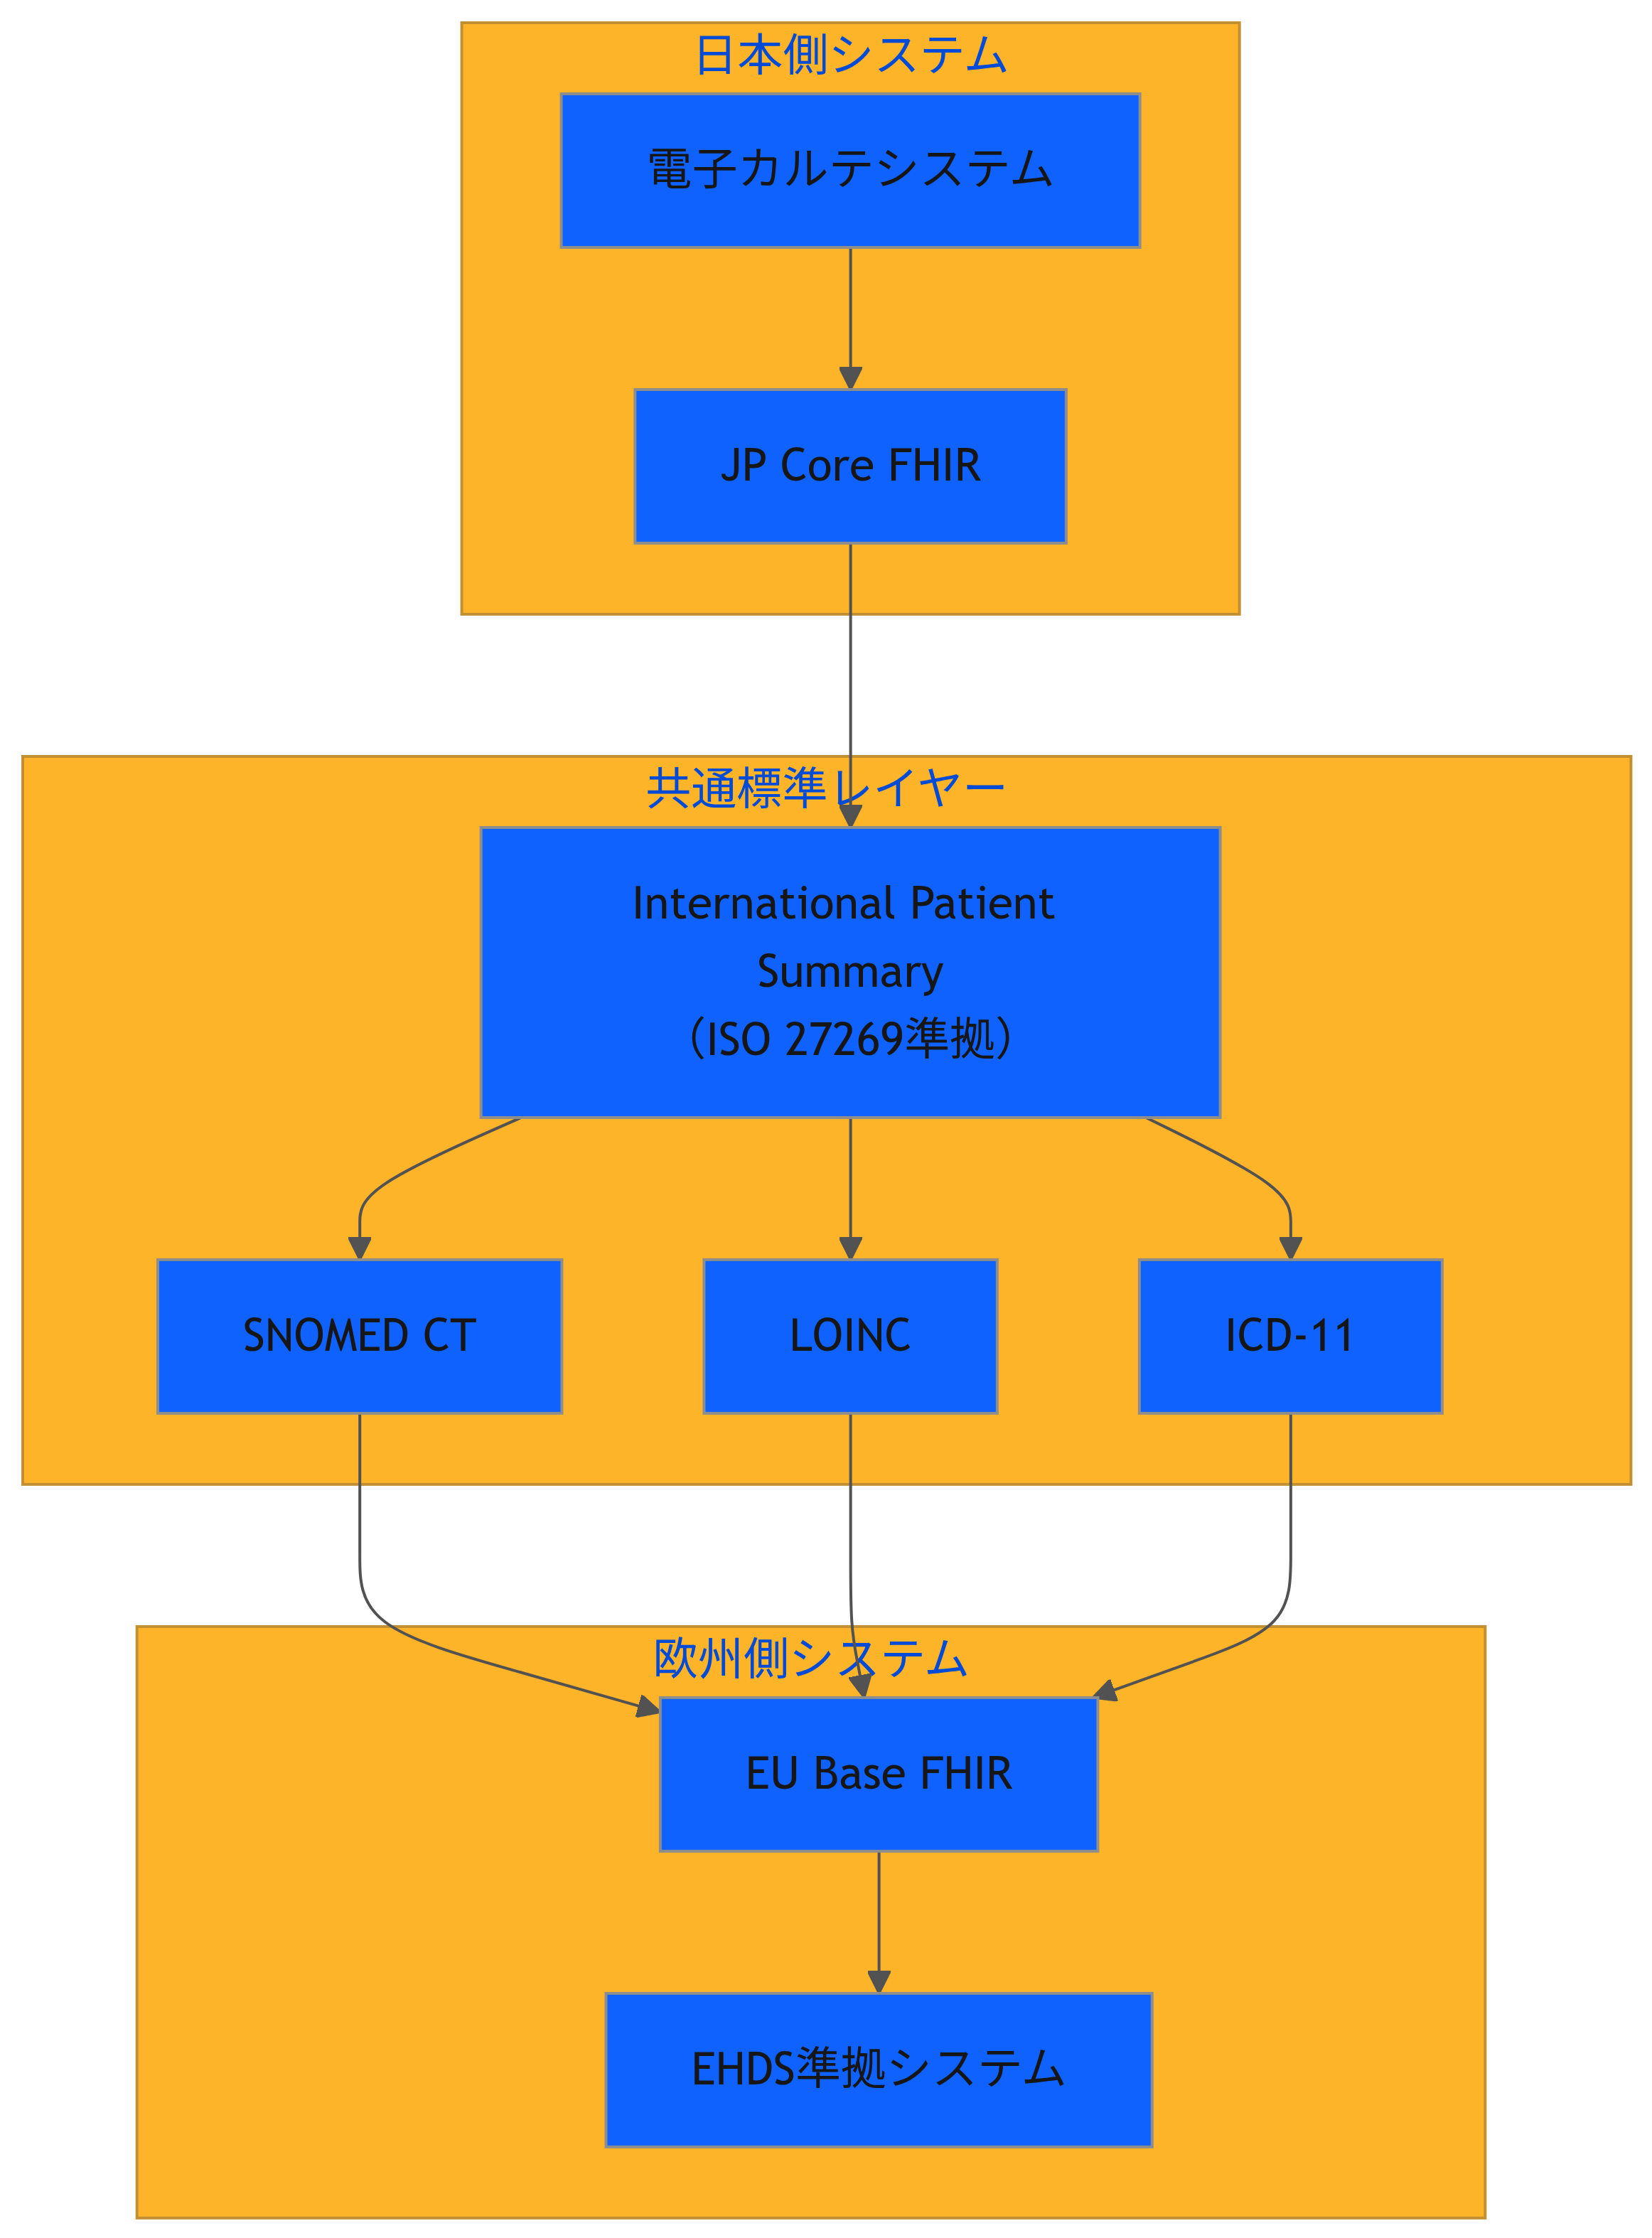
\includegraphics[width=6.06in,height=8.21in]{03-technical-architecture_files/figure-latex/mermaid-figure-5.png}

IPS共通プロファイル方式による日欧相互運用性

\textbf{IPS共通プロファイル方式の特徴}：

\begin{enumerate}
\def\labelenumi{\arabic{enumi}.}
\item
  \textbf{標準化された変換プロセス}：

  \begin{itemize}
  \tightlist
  \item
    段階1：JP Core → IPS変換（日本独自要素を国際標準要素にマッピング）
  \item
    段階2：IPS → EU Base変換（国際標準から欧州仕様へ適応）
  \end{itemize}
\item
  \textbf{必須データ要素の統一}：

  \begin{itemize}
  \tightlist
  \item
    アレルギー・不耐性情報（AllergyIntolerance）
  \item
    服薬歴（MedicationSummary）
  \item
    既往歴・現病歴（ProblemList）
  \end{itemize}
\item
  \textbf{実用的な変換例}：

\begin{Shaded}
\begin{Highlighting}[]
\ErrorTok{//} \ErrorTok{JP} \ErrorTok{Core} \ErrorTok{→} \ErrorTok{IPS変換}
\FunctionTok{\{}
  \DataTypeTok{"resourceType"}\FunctionTok{:} \StringTok{"AllergyIntolerance"}\FunctionTok{,}
  \DataTypeTok{"code"}\FunctionTok{:} \FunctionTok{\{}
    \DataTypeTok{"coding"}\FunctionTok{:} \OtherTok{[}
      \FunctionTok{\{}
        \DataTypeTok{"system"}\FunctionTok{:} \StringTok{"http://jpfhir.jp/fhir/core/CodeSystem/JP\_AllergyIntolerance\_VS"}\FunctionTok{,}
        \DataTypeTok{"code"}\FunctionTok{:} \StringTok{"PENICILLIN\_ALLERGY\_JP"}
      \FunctionTok{\}}
    \OtherTok{]}
  \FunctionTok{\}}
\FunctionTok{\}}

\ErrorTok{//} \ErrorTok{IPS標準形式}
\FunctionTok{\{}
  \DataTypeTok{"resourceType"}\FunctionTok{:} \StringTok{"AllergyIntolerance"}\FunctionTok{,} 
  \DataTypeTok{"code"}\FunctionTok{:} \FunctionTok{\{}
    \DataTypeTok{"coding"}\FunctionTok{:} \OtherTok{[}
      \FunctionTok{\{}
        \DataTypeTok{"system"}\FunctionTok{:} \StringTok{"http://snomed.info/sct"}\FunctionTok{,}
        \DataTypeTok{"code"}\FunctionTok{:} \StringTok{"294505008"}\FunctionTok{,}
        \DataTypeTok{"display"}\FunctionTok{:} \StringTok{"Allergy to penicillin"}
      \FunctionTok{\}}
    \OtherTok{]}
  \FunctionTok{\}}
\FunctionTok{\}}
\end{Highlighting}
\end{Shaded}
\end{enumerate}

\subsubsection{長期実装例：分散型標準化アーキテクチャ}\label{ux9577ux671fux5b9fux88c5ux4f8bux5206ux6563ux578bux6a19ux6e96ux5316ux30a2ux30fcux30adux30c6ux30afux30c1ux30e3}

長期フェーズでは、単一障害点を排除し、各国のデータ主権を完全に保護しながら、標準化されたプロトコルによる完全な相互運用性を実現する：

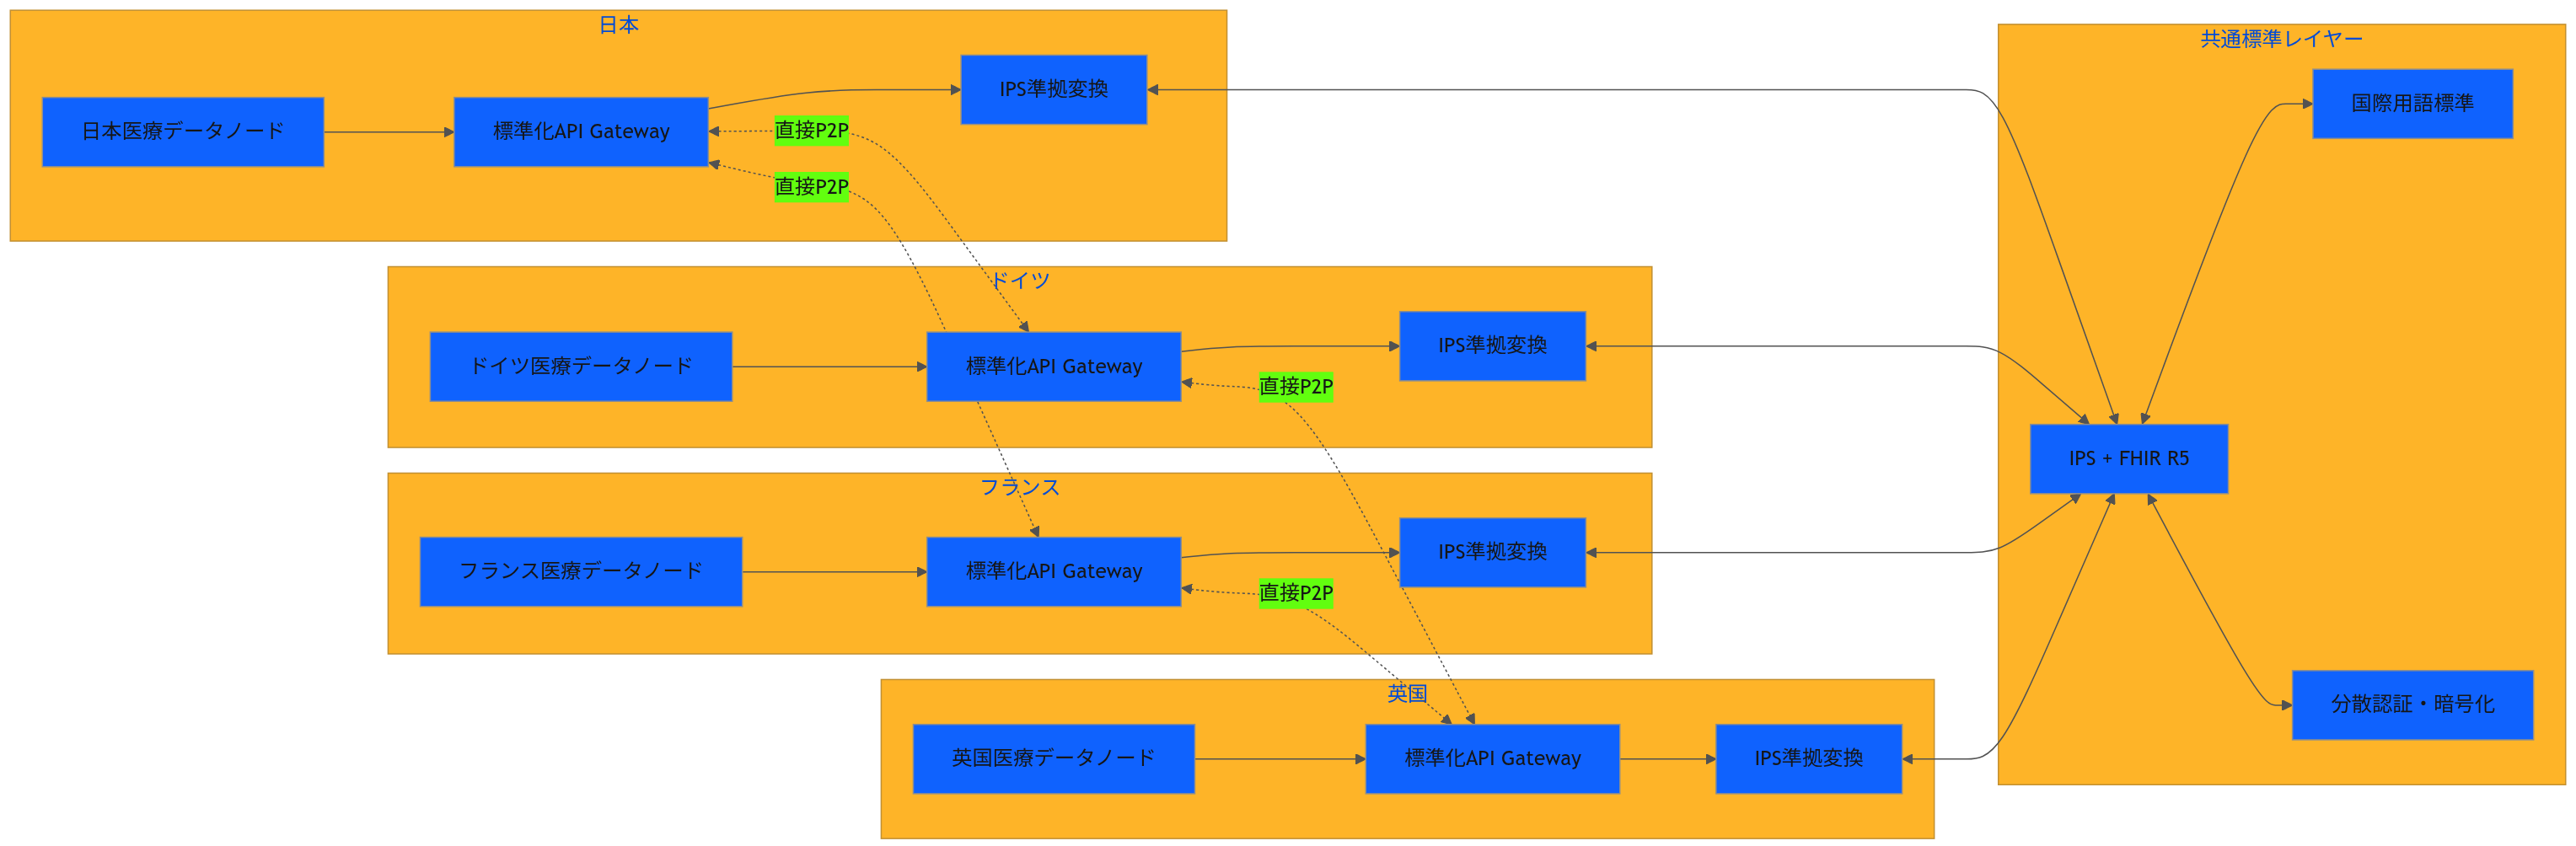
\includegraphics[width=20.92in,height=6.9in]{03-technical-architecture_files/figure-latex/mermaid-figure-4.png}

分散型メッシュ相互運用アーキテクチャ

\textbf{分散型標準化方式の特徴}：

\begin{enumerate}
\def\labelenumi{\arabic{enumi}.}
\tightlist
\item
  \textbf{完全な分散アーキテクチャ}：

  \begin{itemize}
  \tightlist
  \item
    単一障害点（SPOF）の完全排除
  \item
    各国のデータ主権の完全保護
  \item
    スケーラブルなP2P接続
  \end{itemize}
\item
  \textbf{標準化による相互運用性}：

  \begin{itemize}
  \tightlist
  \item
    IPS（International Patient Summary）完全準拠
  \item
    FHIR R5による次世代相互運用性
  \item
    AI支援による自動用語マッピング
  \end{itemize}
\item
  \textbf{実用的なデータ活用シナリオ}：

  \begin{itemize}
  \tightlist
  \item
    \textbf{ケース：リアルタイム緊急医療}

    \begin{itemize}
    \tightlist
    \item
      日本人患者がドイツで緊急搬送
    \item
      ドイツ→日本への直接API呼び出し
    \item
      リアルタイムでの患者サマリー取得
    \end{itemize}
  \item
    \textbf{ケース：分散型臨床研究}

    \begin{itemize}
    \tightlist
    \item
      希少疾患の国際共同研究
    \item
      各国が自国データを保持したまま参加
    \item
      標準化されたクエリで統計的分析を実施
    \end{itemize}
  \item
    \textbf{ケース：パンデミック対応}

    \begin{itemize}
    \tightlist
    \item
      新興感染症の早期警戒システム
    \item
      各国の疫学データを標準フォーマットで共有
    \item
      分散合意アルゴリズムによる迅速な意思決定
    \end{itemize}
  \end{itemize}
\end{enumerate}

\textbf{技術的な実現要素}：

\begin{itemize}
\tightlist
\item
  \textbf{分散ID管理}：各国の認証システムが直接連携
\item
  \textbf{エッジコンピューティング}：データ処理を各国内で完結
\item
  \textbf{ブロックチェーン監査}：データアクセス履歴の透明性確保
\item
  \textbf{AI支援変換}：用語・プロファイル変換の完全自動化
\end{itemize}

\begin{tcolorbox}[enhanced jigsaw, toprule=.15mm, bottomtitle=1mm, coltitle=black, left=2mm, opacityback=0, arc=.35mm, colbacktitle=quarto-callout-note-color!10!white, colback=white, opacitybacktitle=0.6, bottomrule=.15mm, rightrule=.15mm, breakable, title=\textcolor{quarto-callout-note-color}{\faInfo}\hspace{0.5em}{Note}, toptitle=1mm, titlerule=0mm, colframe=quarto-callout-note-color-frame, leftrule=.75mm]

\textbf{段階的発展の重要性}：短期のゲートウェイ方式で基本的な相互運用性を確立し、中期のIPS方式で標準化を進め、長期の分散型方式で持続可能で拡張性のある国際医療データ連携基盤を構築する。この段階的アプローチにより、各段階での学習と改善を重ねながら、最終的に単一障害点のない堅牢なシステムを実現できる。

\end{tcolorbox}

\section{セキュリティとプライバシー}\label{ux30bbux30adux30e5ux30eaux30c6ux30a3ux3068ux30d7ux30e9ux30a4ux30d0ux30b7ux30fc}

\subsection{技術的保護措置}\label{ux6280ux8853ux7684ux4fddux8b77ux63aaux7f6e}

\textbf{事実}：EHDS規則（EU
2025/327）第50条では、「健康データアクセス機関は、セキュアプロセッシング環境を通じてのみ電子健康データへのアクセスを提供しなければならない」と定めており{[}1{]},
{[}13{]}、技術的・組織的措置、セキュリティ、相互運用性要件の実装が求められている。詳細な技術仕様は2027年3月までに採択される実施法令で規定される予定である。

\subsubsection{EHDS実装の参考となるセキュリティアプローチ}\label{ehdsux5b9fux88c5ux306eux53c2ux8003ux3068ux306aux308bux30bbux30adux30e5ux30eaux30c6ux30a3ux30a2ux30d7ux30edux30fcux30c1}

\begin{tcolorbox}[enhanced jigsaw, toprule=.15mm, bottomtitle=1mm, coltitle=black, left=2mm, opacityback=0, arc=.35mm, colbacktitle=quarto-callout-warning-color!10!white, colback=white, opacitybacktitle=0.6, bottomrule=.15mm, rightrule=.15mm, breakable, title=\textcolor{quarto-callout-warning-color}{\faExclamationTriangle}\hspace{0.5em}{Warning}, toptitle=1mm, titlerule=0mm, colframe=quarto-callout-warning-color-frame, leftrule=.75mm]

\textbf{注意}：以下のセキュリティ技術は、ENISA（欧州サイバーセキュリティ庁）のデータ保護エンジニアリングガイドライン{[}17{]}および医療データ保護における国際的なベストプラクティスに基づく推奨事項である。EHDS規則の具体的な技術仕様は2027年3月までに採択される実施法令で定められる予定であり、実装時は最新の公式仕様を確認すること。

\end{tcolorbox}

\textbf{1. データ暗号化要件}

ENISAのデータ保護エンジニアリング報告書によると、医療データの保護において以下の暗号化アプローチが推奨される{[}17{]}：

\begin{itemize}
\tightlist
\item
  \textbf{保存時暗号化}：

  \begin{itemize}
  \tightlist
  \item
    強力な暗号化アルゴリズムの使用（AES-256等）
  \item
    ファイルシステムレベル、データベースレベル、アプリケーションレベルでの暗号化オプション（セクション5.2）{[}17{]}
  \end{itemize}
\item
  \textbf{転送時暗号化}：

  \begin{itemize}
  \tightlist
  \item
    TLS 1.2以上の使用（TLS 1.3を強く推奨）
  \item
    エンドツーエンド暗号化（E2EE）の実装検討（セクション5.1.1）{[}17{]}
  \end{itemize}
\item
  \textbf{鍵管理}：

  \begin{itemize}
  \tightlist
  \item
    暗号鍵の安全な生成、保管、ローテーション
  \item
    HSM（Hardware Security Module）の活用を推奨
  \end{itemize}
\item
  \textbf{暗号化アルゴリズム}：

  \begin{itemize}
  \tightlist
  \item
    各国のサイバーセキュリティ機関が承認したアルゴリズムの使用
  \end{itemize}
\end{itemize}

\textbf{2. アイデンティティ・アクセス管理（IAM）}

ISO/IEC 27001およびOWASP（Open Web Application Security
Project）のガイドラインに基づき、以下のIAM実装が推奨される{[}33{]},
{[}34{]}：

\begin{itemize}
\tightlist
\item
  \textbf{認証方式の強化}：

  \begin{itemize}
  \tightlist
  \item
    多要素認証（MFA）の実装
  \item
    生体認証技術の活用検討
  \item
    リスクベース認証の導入
  \end{itemize}
\item
  \textbf{認可フレームワーク}：

  \begin{itemize}
  \tightlist
  \item
    OAuth 2.0およびOpenID Connectなどの標準プロトコル{[}35{]}, {[}36{]}
  \item
    患者による同意管理機能
  \item
    役割ベースアクセス制御（RBAC）
  \end{itemize}
\end{itemize}

\textbf{3. ネットワークセキュリティ}

NIST Special Publication
800-207「ゼロトラストアーキテクチャ」に基づく実装が推奨される{[}37{]}：

\begin{itemize}
\tightlist
\item
  \textbf{ゼロトラストの原則}：

  \begin{itemize}
  \tightlist
  \item
    「決して信頼せず、常に検証する」アプローチ
  \item
    ネットワークセグメンテーション
  \item
    継続的な信頼性評価
  \end{itemize}
\item
  \textbf{ネットワーク保護}：

  \begin{itemize}
  \tightlist
  \item
    医療データゾーンの分離
  \item
    ファイアウォールによる多層防御
  \item
    VPN等による安全な接続
  \end{itemize}
\end{itemize}

\textbf{4. 監査・コンプライアンス}

ISO/IEC
27018（クラウドにおける個人情報保護）およびGDPR第32条の技術的措置に準拠{[}19{]},
{[}38{]}：

\begin{itemize}
\tightlist
\item
  \textbf{ロギング要件}：

  \begin{itemize}
  \tightlist
  \item
    データアクセスの包括的な記録
  \item
    ログの完全性と改ざん防止
  \item
    規制要件に応じた保存期間
  \end{itemize}
\item
  \textbf{監査機能}：

  \begin{itemize}
  \tightlist
  \item
    監査ログの定期的レビュー
  \item
    セキュリティ情報イベント管理（SIEM）の活用
  \item
    異常検知とアラート機能
  \end{itemize}
\end{itemize}

\textbf{5. データ保護・プライバシー}

ISO/IEC
20889（プライバシー強化のためのデ・アイデンティフィケーション技術）に基づく実装{[}39{]}：

\begin{itemize}
\tightlist
\item
  \textbf{仮名化・匿名化}：

  \begin{itemize}
  \tightlist
  \item
    データの再識別リスクを最小化する技術の適用
  \item
    k-匿名性などのプライバシー保護手法{[}40{]}
  \item
    差分プライバシーの検討{[}41{]}
  \end{itemize}
\item
  \textbf{データガバナンス}：

  \begin{itemize}
  \tightlist
  \item
    目的制限の原則の遵守
  \item
    データ保持ポリシーの策定と実施
  \item
    不要データの安全な削除手順
  \end{itemize}
\end{itemize}

\textbf{6. インシデント対応}

ISO/IEC
27035（情報セキュリティインシデント管理）に準拠した体制構築{[}42{]}：

\begin{itemize}
\tightlist
\item
  \textbf{監視体制}：

  \begin{itemize}
  \tightlist
  \item
    セキュリティ監視の実施
  \item
    脅威インテリジェンスの活用
  \item
    インシデント検知と対応の迅速化
  \end{itemize}
\item
  \textbf{対応計画}：

  \begin{itemize}
  \tightlist
  \item
    インシデント対応手順の文書化
  \item
    GDPR等の規制に基づく通知要件（72時間以内）
  \item
    事業継続計画との統合
  \end{itemize}
\end{itemize}

\textbf{7. セキュリティ評価・認証}

\begin{itemize}
\tightlist
\item
  \textbf{推奨される認証}：

  \begin{itemize}
  \tightlist
  \item
    ISO/IEC 27001（情報セキュリティマネジメント）{[}33{]}
  \item
    ISO/IEC 27017（クラウドセキュリティ）{[}43{]}
  \item
    ISO/IEC 27701（プライバシー情報マネジメント）{[}44{]}
  \end{itemize}
\item
  \textbf{継続的改善}：

  \begin{itemize}
  \tightlist
  \item
    定期的なセキュリティ評価
  \item
    脆弱性管理プログラム
  \item
    セキュリティ教育と訓練
  \end{itemize}
\end{itemize}

\subsection{プライバシー強化技術（PETs）}\label{ux30d7ux30e9ux30a4ux30d0ux30b7ux30fcux5f37ux5316ux6280ux8853pets}

\begin{tcolorbox}[enhanced jigsaw, toprule=.15mm, bottomtitle=1mm, coltitle=black, left=2mm, opacityback=0, arc=.35mm, colbacktitle=quarto-callout-note-color!10!white, colback=white, opacitybacktitle=0.6, bottomrule=.15mm, rightrule=.15mm, breakable, title=\textcolor{quarto-callout-note-color}{\faInfo}\hspace{0.5em}{Note}, toptitle=1mm, titlerule=0mm, colframe=quarto-callout-note-color-frame, leftrule=.75mm]

\textbf{注記}：EHDSの二次利用において、データ保護の観点から匿名化・仮名化などのデータ最小化措置とセキュアプロセッシング環境での処理が重要な役割を果たすとされている。学術研究では、これらの措置の効果的で一貫性のある実装のために、より明確な規制要件の必要性が指摘されている{[}45{]}。

\end{tcolorbox}

\subsubsection{医療データ研究で検討されているPETs}\label{ux533bux7642ux30c7ux30fcux30bfux7814ux7a76ux3067ux691cux8a0eux3055ux308cux3066ux3044ux308bpets}

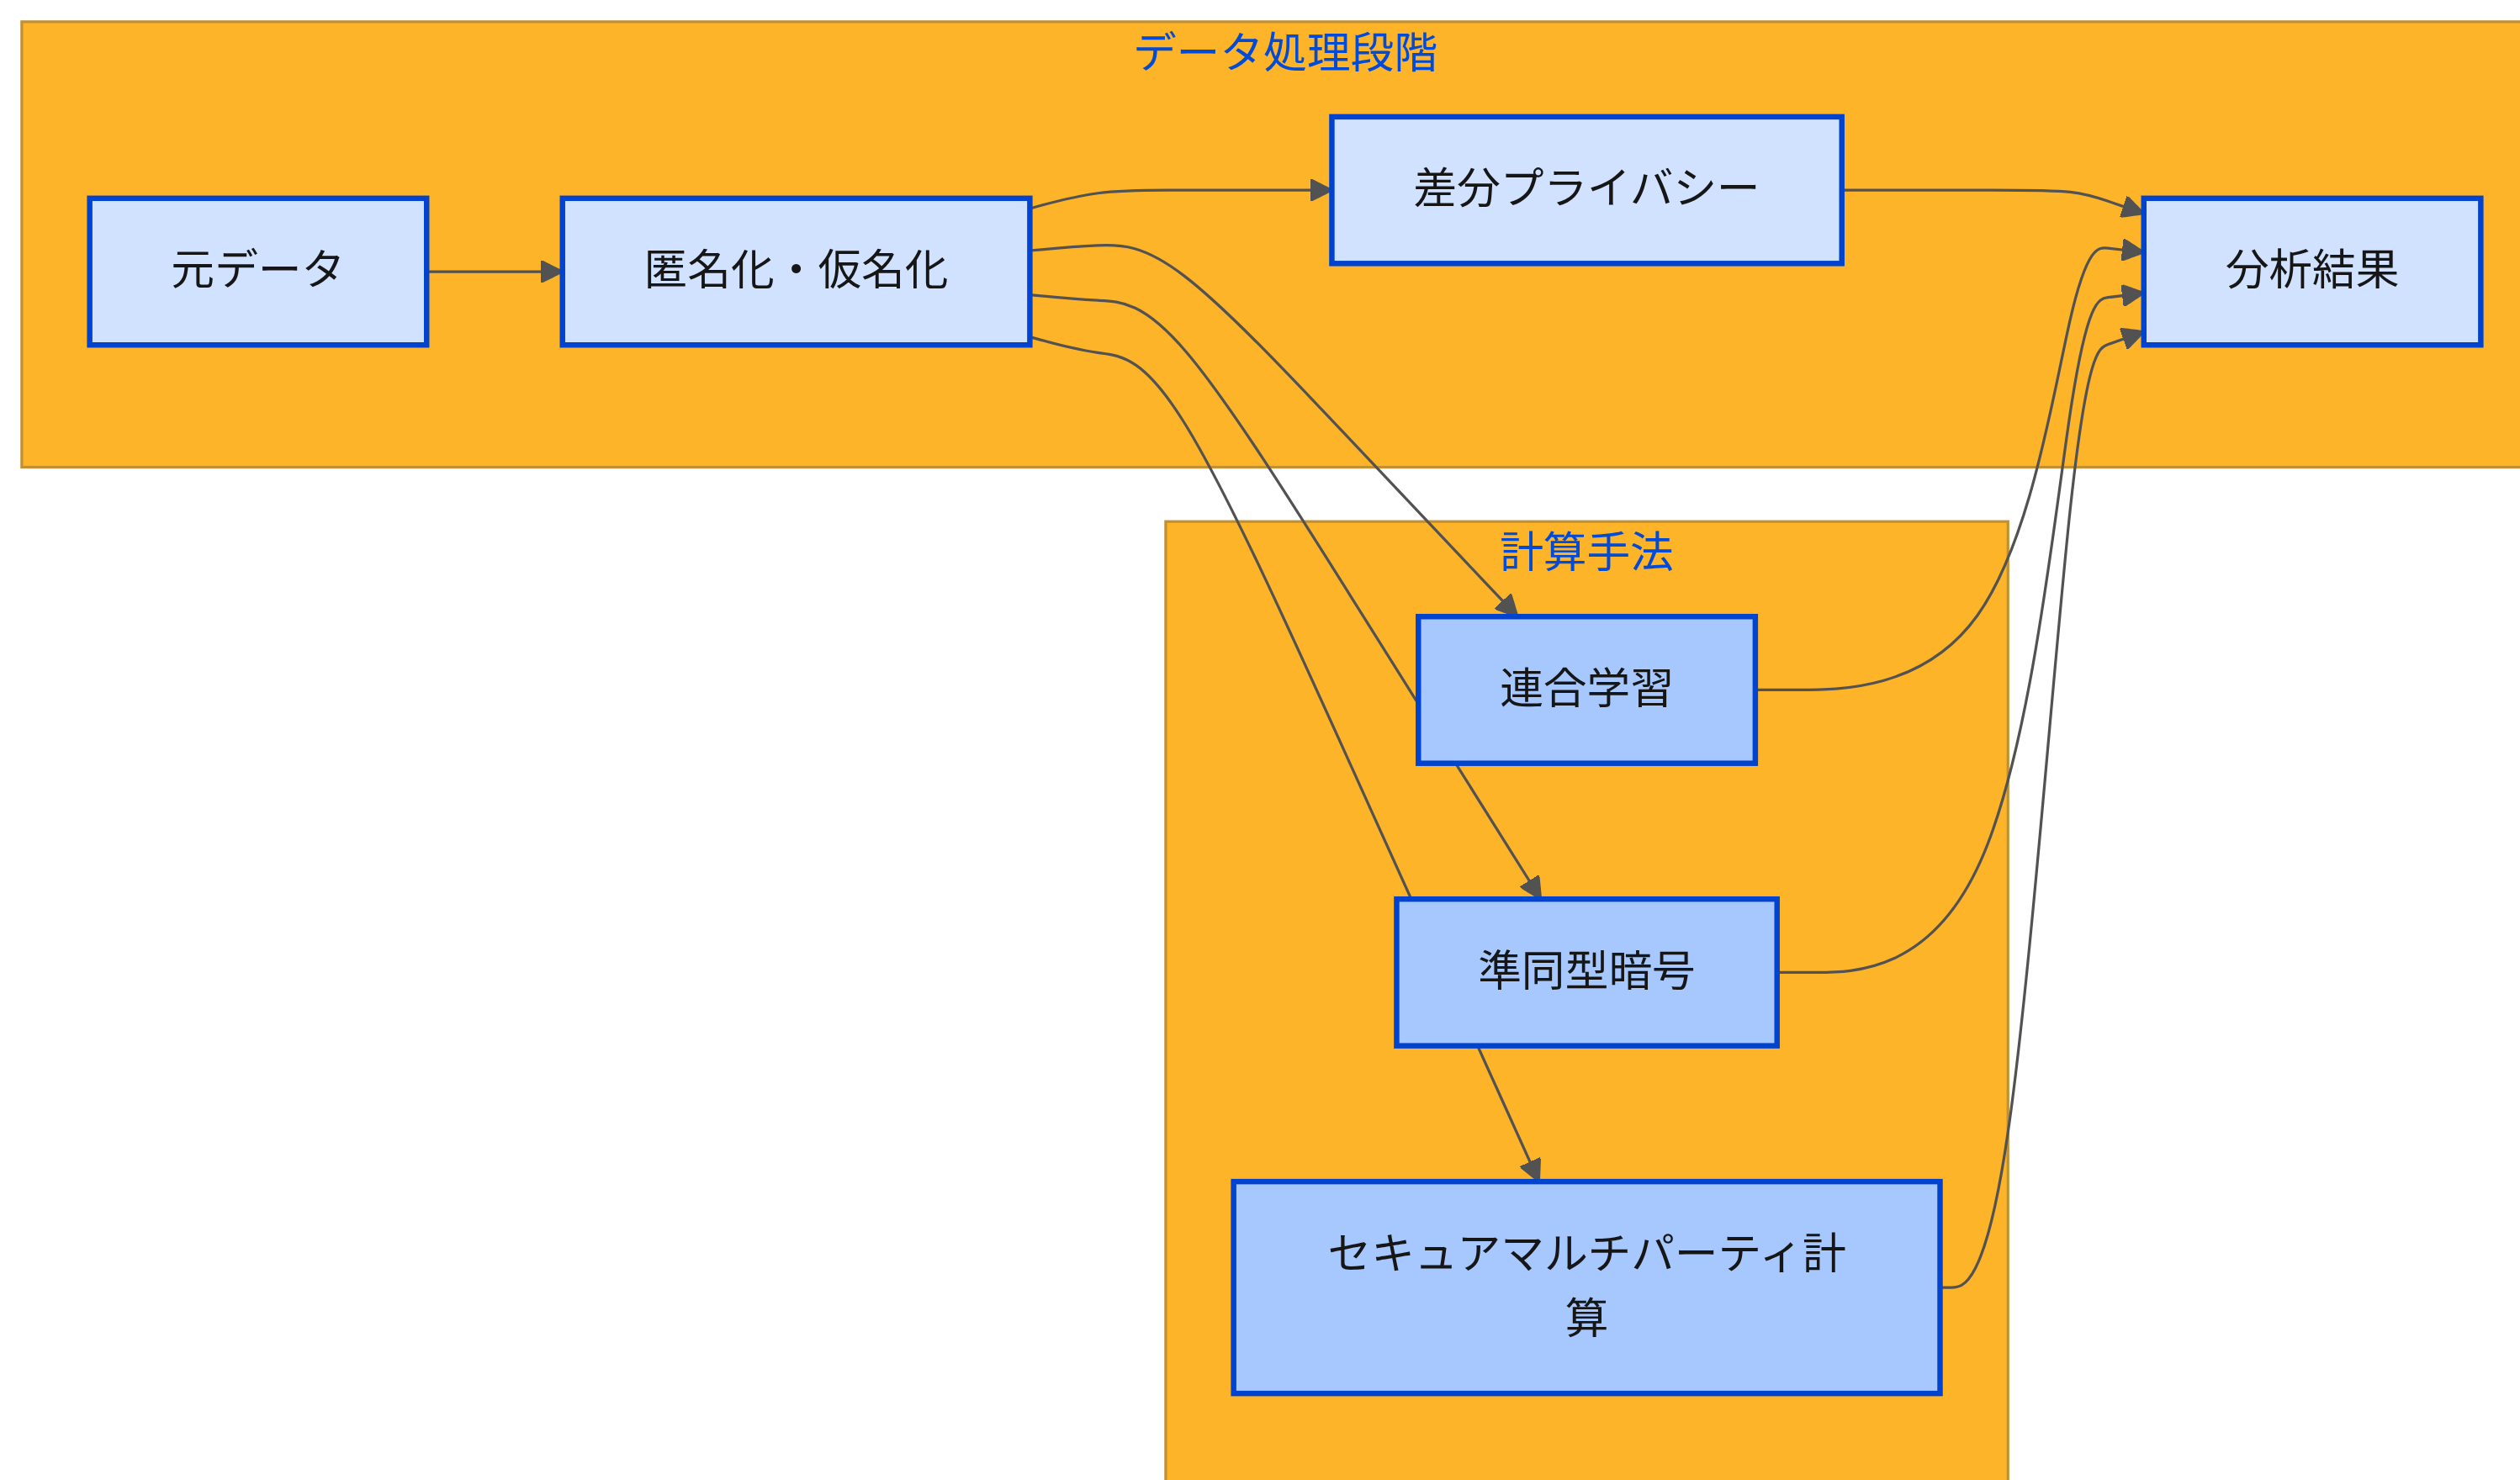
\includegraphics[width=9.85in,height=5.79in]{03-technical-architecture_files/figure-latex/mermaid-figure-3.png}

医療データの二次利用で活用が検討されているプライバシー強化技術

\begin{tcolorbox}[enhanced jigsaw, toprule=.15mm, bottomtitle=1mm, coltitle=black, left=2mm, opacityback=0, arc=.35mm, colbacktitle=quarto-callout-note-color!10!white, colback=white, opacitybacktitle=0.6, bottomrule=.15mm, rightrule=.15mm, breakable, title=\textcolor{quarto-callout-note-color}{\faInfo}\hspace{0.5em}{Note}, toptitle=1mm, titlerule=0mm, colframe=quarto-callout-note-color-frame, leftrule=.75mm]

\textbf{注記}：上記の技術は、医療データのプライバシー保護に関する学術研究や国際的な技術コミュニティで検討されている手法である。実際の実装においては、各国の規制要件と技術的制約を考慮した上で、適切な技術の選択と組み合わせが必要となる。

\end{tcolorbox}

\section{クラウドインフラストラクチャ}\label{ux30afux30e9ux30a6ux30c9ux30a4ux30f3ux30d5ux30e9ux30b9ux30c8ux30e9ux30afux30c1ux30e3}

\subsection{要件と認証}\label{ux8981ux4ef6ux3068ux8a8dux8a3c}

\begin{tcolorbox}[enhanced jigsaw, toprule=.15mm, bottomtitle=1mm, coltitle=black, left=2mm, opacityback=0, arc=.35mm, colbacktitle=quarto-callout-note-color!10!white, colback=white, opacitybacktitle=0.6, bottomrule=.15mm, rightrule=.15mm, breakable, title=\textcolor{quarto-callout-note-color}{\faInfo}\hspace{0.5em}{Note}, toptitle=1mm, titlerule=0mm, colframe=quarto-callout-note-color-frame, leftrule=.75mm]

\textbf{注記}：主要クラウドプロバイダー（AWS、Azure、Google
Cloud等）は、EHDS要件に対応したクラウドサービスの提供に向けて準備を進めている。各プロバイダーは、EU域内でのデータ保存、GDPR準拠、適切なセキュリティ認証の取得などを通じて、医療データの安全な処理環境を提供することが期待されている。

\end{tcolorbox}

\textbf{クラウドプロバイダー要件}：

\begin{enumerate}
\def\labelenumi{\arabic{enumi}.}
\tightlist
\item
  \textbf{データローカライゼーション}

  \begin{itemize}
  \tightlist
  \item
    EU域内でのデータ保存
  \item
    データレジデンシーの保証
  \item
    越境転送の制限
  \end{itemize}
\item
  \textbf{セキュリティ認証}

  \begin{itemize}
  \tightlist
  \item
    ISO 27001/27017/27018
  \item
    SOC 2 Type II
  \item
    CSA STAR Level 2
  \end{itemize}
\item
  \textbf{コンプライアンス}

  \begin{itemize}
  \tightlist
  \item
    GDPR完全準拠
  \item
    EHDS特有要件への対応
  \item
    定期的な第三者監査
  \end{itemize}
\end{enumerate}

\subsection{ハイブリッドクラウド戦略}\label{ux30cfux30a4ux30d6ux30eaux30c3ux30c9ux30afux30e9ux30a6ux30c9ux6226ux7565}

\textbf{考察}：医療分野では、セキュリティ要件、規制遵守、レガシーシステムとの統合などの課題から、多くの医療機関がハイブリッドクラウド戦略を採用している{[}46{]}。WHOのデジタルヘルス戦略2020-2025では、各国が既存のハードウェアと接続性の包括的な評価を行い、デジタル化を推進するためのインフラストラクチャのニーズとソリューションを特定すること、そして柔軟なデジタルインフラストラクチャを構築することの重要性が強調されている{[}47{]}。この文脈において、機密性の高い患者データはオンプレミスで管理しつつ、研究用の匿名化データや災害復旧システムはクラウドを活用するハイブリッド戦略は、各国の状況に応じた現実的なアプローチとして位置づけられる。

\textbf{推奨アーキテクチャ}：

\begin{itemize}
\tightlist
\item
  \textbf{オンプレミス}：機密性の高い患者データ、レガシーシステム
\item
  \textbf{プライベートクラウド}：院内システム、部門システム
\item
  \textbf{パブリッククラウド}：匿名化データ、研究用データセット
\end{itemize}

\section{API設計とマイクロサービス}\label{apiux8a2dux8a08ux3068ux30deux30a4ux30afux30edux30b5ux30fcux30d3ux30b9}

\subsection{RESTful
API設計原則}\label{restful-apiux8a2dux8a08ux539fux5247}

\subsubsection{FHIRベースのRESTful
API実装}\label{fhirux30d9ux30fcux30b9ux306erestful-apiux5b9fux88c5}

\textbf{事実}：HL7 FHIRは、RESTful
アーキテクチャ原則に基づいて設計された医療データ交換標準であり、EHDSの技術実装において中核的な役割を果たしている{[}23{]}。FHIRは、HTTPプロトコルを使用し、リソースベースのアプローチで医療情報を構造化・交換する。

\textbf{FHIRのRESTful設計原則}：

\begin{enumerate}
\def\labelenumi{\arabic{enumi}.}
\item
  \textbf{リソース指向アーキテクチャ}

  \begin{itemize}
  \tightlist
  \item
    すべての医療データは「リソース」として表現（Patient、Observation、MedicationRequest等）
  \item
    各リソースは一意のURL（論理ID）でアクセス可能
  \item
    標準的なHTTPメソッド（GET、POST、PUT、DELETE）による操作
  \end{itemize}
\item
  \textbf{統一インターフェース}

\begin{Shaded}
\begin{Highlighting}[]
\NormalTok{\# 患者情報の取得}
\NormalTok{GET /fhir/Patient/123}
\NormalTok{Accept: application/fhir+json}

\NormalTok{\# 検査結果の検索}
\NormalTok{GET /fhir/Observation?patient=123\&code=http://loinc.org|2345{-}7}

\NormalTok{\# 新規処方の登録}
\NormalTok{POST /fhir/MedicationRequest}
\NormalTok{Content{-}Type: application/fhir+json}
\end{Highlighting}
\end{Shaded}
\item
  \textbf{ステートレス通信}

  \begin{itemize}
  \tightlist
  \item
    各リクエストは独立して処理可能
  \item
    セッション状態をサーバー側で保持しない
  \item
    認証トークンによる状態管理
  \end{itemize}
\end{enumerate}

\textbf{FHIR標準に基づくAPI実装パターン}：

\begin{tcolorbox}[enhanced jigsaw, toprule=.15mm, bottomtitle=1mm, coltitle=black, left=2mm, opacityback=0, arc=.35mm, colbacktitle=quarto-callout-note-color!10!white, colback=white, opacitybacktitle=0.6, bottomrule=.15mm, rightrule=.15mm, breakable, title=\textcolor{quarto-callout-note-color}{\faInfo}\hspace{0.5em}{Note}, toptitle=1mm, titlerule=0mm, colframe=quarto-callout-note-color-frame, leftrule=.75mm]

\textbf{注記}：以下の例は、HL7
FHIR仕様書{[}23{]}に定義されている標準的なRESTful
APIパターンを、EHDS実装の文脈で示したものである。実際の実装では、各国の規制要件やシステム要件に応じた調整が必要となる。

\end{tcolorbox}

\begin{Shaded}
\begin{Highlighting}[]
\CommentTok{\# OpenAPI 3.0形式でのFHIR API定義例}
\FunctionTok{openapi}\KeywordTok{:}\AttributeTok{ }\FloatTok{3.0.0}
\FunctionTok{info}\KeywordTok{:}
\AttributeTok{  }\FunctionTok{title}\KeywordTok{:}\AttributeTok{ FHIR API Example for EHDS}
\AttributeTok{  }\FunctionTok{version}\KeywordTok{:}\AttributeTok{ }\FloatTok{1.0.0}
\FunctionTok{paths}\KeywordTok{:}
\AttributeTok{  }\FunctionTok{/fhir/Patient/\{id\}}\KeywordTok{:}
\AttributeTok{    }\FunctionTok{get}\KeywordTok{:}
\AttributeTok{      }\FunctionTok{summary}\KeywordTok{:}\AttributeTok{ 患者情報取得}
\AttributeTok{      }\FunctionTok{parameters}\KeywordTok{:}
\AttributeTok{        }\KeywordTok{{-}}\AttributeTok{ }\FunctionTok{name}\KeywordTok{:}\AttributeTok{ id}
\AttributeTok{          }\FunctionTok{in}\KeywordTok{:}\AttributeTok{ path}
\AttributeTok{          }\FunctionTok{required}\KeywordTok{:}\AttributeTok{ }\CharTok{true}
\AttributeTok{          }\FunctionTok{schema}\KeywordTok{:}
\AttributeTok{            }\FunctionTok{type}\KeywordTok{:}\AttributeTok{ string}
\AttributeTok{      }\FunctionTok{security}\KeywordTok{:}
\AttributeTok{        }\KeywordTok{{-}}\AttributeTok{ }\FunctionTok{OAuth2}\KeywordTok{:}\AttributeTok{ }\KeywordTok{[}\AttributeTok{patient/Patient.read}\KeywordTok{]}
\AttributeTok{      }\FunctionTok{responses}\KeywordTok{:}
\AttributeTok{        }\FunctionTok{200}\KeywordTok{:}
\AttributeTok{          }\FunctionTok{description}\KeywordTok{:}\AttributeTok{ 患者リソース}
\AttributeTok{          }\FunctionTok{content}\KeywordTok{:}
\AttributeTok{            }\FunctionTok{application/fhir+json}\KeywordTok{:}
\AttributeTok{              }\FunctionTok{schema}\KeywordTok{:}
\AttributeTok{                }\FunctionTok{$ref}\KeywordTok{:}\AttributeTok{ }\StringTok{\textquotesingle{}http://hl7.org/fhir/patient.schema.json\textquotesingle{}}
\end{Highlighting}
\end{Shaded}

\textbf{FHIR仕様に定義された検索機能の活用例}：

FHIR仕様書では、リソース検索のための包括的な検索パラメータが定義されている{[}23{]}。これらを組み合わせることで、複雑な医療データクエリが可能となる：

\begin{Shaded}
\begin{Highlighting}[]
\NormalTok{\# FHIR標準の検索パラメータを使用した例}
\NormalTok{GET /fhir/Observation?}
\NormalTok{  patient=123\&}
\NormalTok{  code=http://loinc.org|2345{-}7\&}
\NormalTok{  date=ge2024{-}01{-}01\&}
\NormalTok{  \_include=Observation:patient}
\end{Highlighting}
\end{Shaded}

\textbf{FHIRトランザクション機能の活用}：

FHIR仕様では、複数のリソース操作を原子的に実行するためのBundleリソースとトランザクション機能が定義されている{[}23{]}。これにより、データの一貫性を保ちながら複数の医療記録を更新できる：

\begin{Shaded}
\begin{Highlighting}[]
\FunctionTok{\{}
  \DataTypeTok{"resourceType"}\FunctionTok{:} \StringTok{"Bundle"}\FunctionTok{,}
  \DataTypeTok{"type"}\FunctionTok{:} \StringTok{"transaction"}\FunctionTok{,}
  \DataTypeTok{"entry"}\FunctionTok{:} \OtherTok{[}
    \FunctionTok{\{}
      \DataTypeTok{"request"}\FunctionTok{:} \FunctionTok{\{}
        \DataTypeTok{"method"}\FunctionTok{:} \StringTok{"POST"}\FunctionTok{,}
        \DataTypeTok{"url"}\FunctionTok{:} \StringTok{"Patient"}
      \FunctionTok{\},}
      \DataTypeTok{"resource"}\FunctionTok{:} \FunctionTok{\{}
        \DataTypeTok{"resourceType"}\FunctionTok{:} \StringTok{"Patient"}\FunctionTok{,}
        \DataTypeTok{"name"}\FunctionTok{:} \OtherTok{[}\FunctionTok{\{}\DataTypeTok{"family"}\FunctionTok{:} \StringTok{"Example"}\FunctionTok{\}}\OtherTok{]}
      \FunctionTok{\}}
    \FunctionTok{\}}
  \OtherTok{]}
\FunctionTok{\}}
\end{Highlighting}
\end{Shaded}

\subsection{マイクロサービスアーキテクチャ}\label{ux30deux30a4ux30afux30edux30b5ux30fcux30d3ux30b9ux30a2ux30fcux30adux30c6ux30afux30c1ux30e3}

\subsubsection{マイクロサービスアーキテクチャの採用}\label{ux30deux30a4ux30afux30edux30b5ux30fcux30d3ux30b9ux30a2ux30fcux30adux30c6ux30afux30c1ux30e3ux306eux63a1ux7528}

\textbf{事実}：HealthData@EU Central Platform Release
3（2025年3月公開）の技術仕様では、「中央プラットフォームはモジュール型アーキテクチャを使用しなければならない」と規定され、さらに「中央プラットフォームは、運用の拡張性と柔軟性を確保するためにマイクロサービスを実装しなければならない」と明記されている。このプラットフォームはDG
SANTEからオープンソースとして公開され、eDelivery、eTranslation、EU
Loginなどの欧州委員会ビルディングブロックを活用している{[}22{]}。

\textbf{考察}：EHDSは公式にマイクロサービスアーキテクチャを採用しており、この設計により以下の利点が実現される：

\begin{enumerate}
\def\labelenumi{\arabic{enumi}.}
\tightlist
\item
  \textbf{独立したデプロイメント}：各モジュールが独立して開発・更新可能
\item
  \textbf{段階的な実装}：2029年、2031年の段階的導入に合わせて必要なモジュールを順次追加
\item
  \textbf{各国の柔軟な実装}：標準化されたインターフェースを維持しながら、各国が独自の実装を選択可能
\item
  \textbf{再利用性の向上}：オープンソースのビルディングブロックとして提供され、各国で再利用可能
\end{enumerate}

\subsubsection{マイクロサービス構成の検討例}\label{ux30deux30a4ux30afux30edux30b5ux30fcux30d3ux30b9ux69cbux6210ux306eux691cux8a0eux4f8b}

\begin{tcolorbox}[enhanced jigsaw, toprule=.15mm, bottomtitle=1mm, coltitle=black, left=2mm, opacityback=0, arc=.35mm, colbacktitle=quarto-callout-note-color!10!white, colback=white, opacitybacktitle=0.6, bottomrule=.15mm, rightrule=.15mm, breakable, title=\textcolor{quarto-callout-note-color}{\faInfo}\hspace{0.5em}{Note}, toptitle=1mm, titlerule=0mm, colframe=quarto-callout-note-color-frame, leftrule=.75mm]

\textbf{注記}：以下は、EHDSの技術要件とマイクロサービスアーキテクチャの一般的な設計パターンに基づいた実装例の一つである。実際の実装は、各国の技術的制約、既存システムとの統合要件、規制要件などに応じて異なる構成となる可能性がある。

\end{tcolorbox}

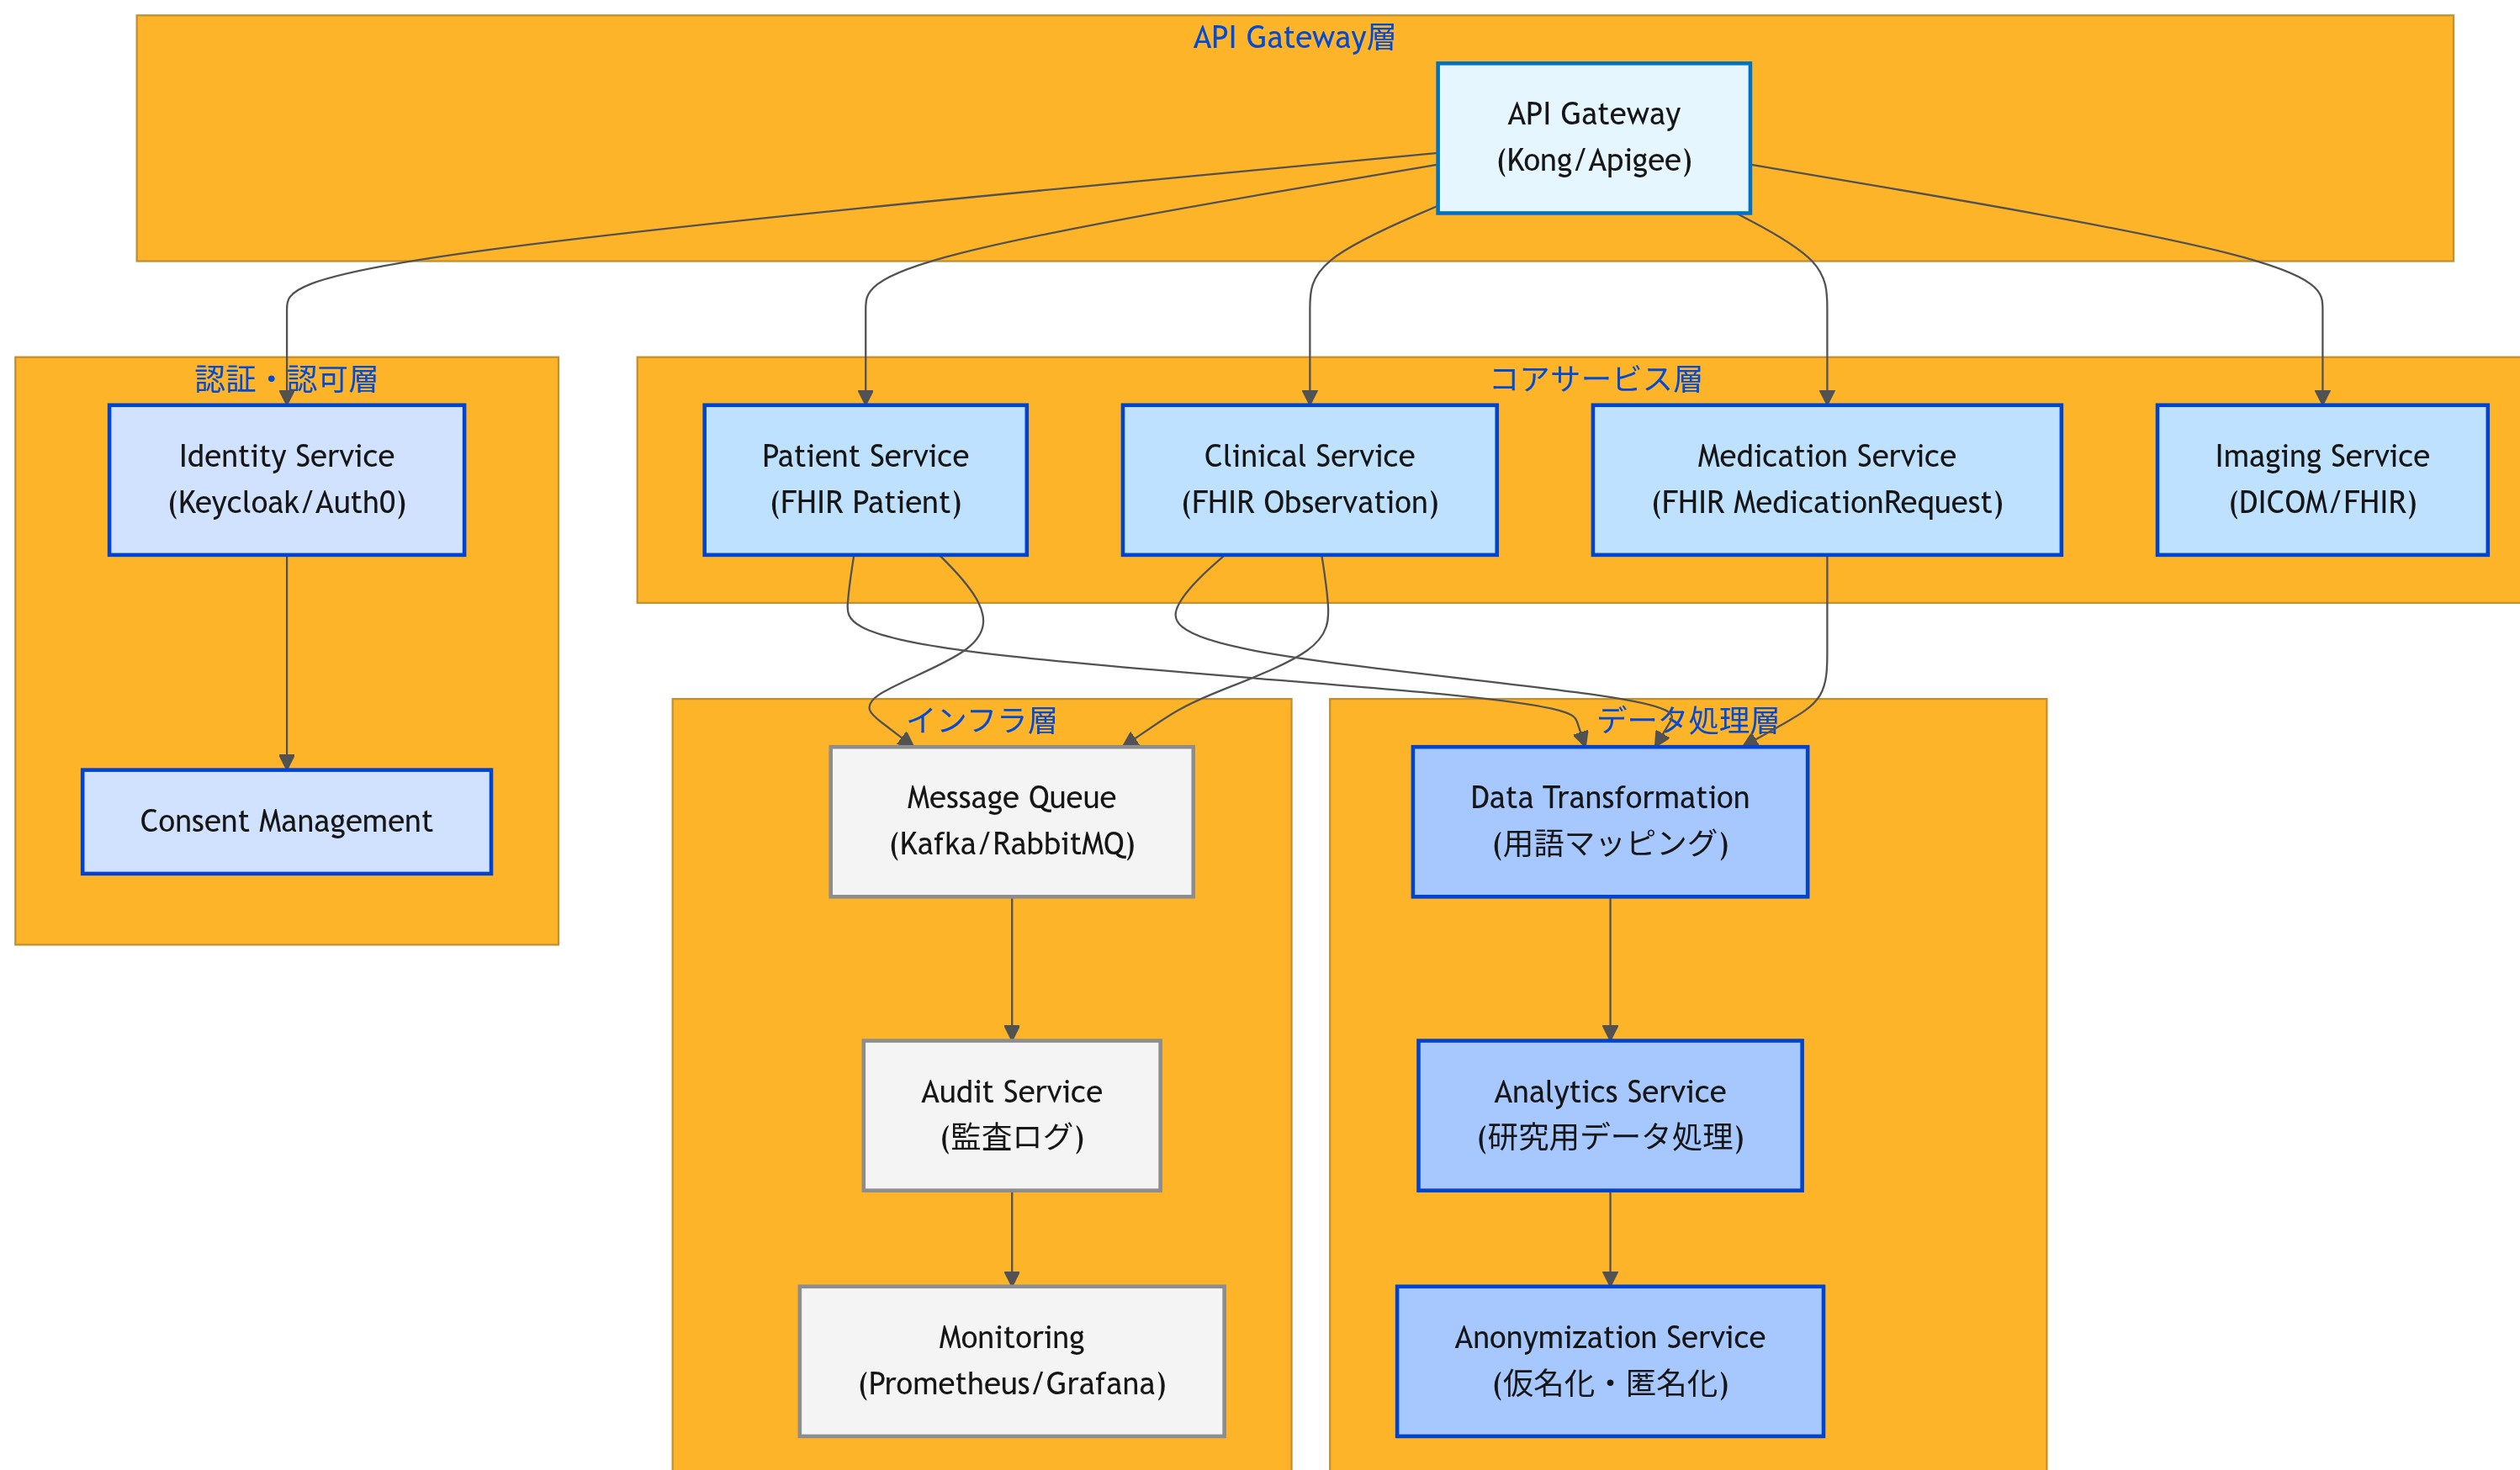
\includegraphics[width=13.94in,height=8.14in]{03-technical-architecture_files/figure-latex/mermaid-figure-2.png}

マイクロサービスアーキテクチャの構成例

\subsubsection{考慮すべきサービス機能の例}\label{ux8003ux616eux3059ux3079ux304dux30b5ux30fcux30d3ux30b9ux6a5fux80fdux306eux4f8b}

\begin{longtable}[]{@{}
  >{\raggedright\arraybackslash}p{(\linewidth - 6\tabcolsep) * \real{0.2787}}
  >{\raggedright\arraybackslash}p{(\linewidth - 6\tabcolsep) * \real{0.2295}}
  >{\raggedright\arraybackslash}p{(\linewidth - 6\tabcolsep) * \real{0.2623}}
  >{\raggedright\arraybackslash}p{(\linewidth - 6\tabcolsep) * \real{0.2295}}@{}}
\toprule\noalign{}
\begin{minipage}[b]{\linewidth}\raggedright
サービスカテゴリ
\end{minipage} & \begin{minipage}[b]{\linewidth}\raggedright
想定される機能
\end{minipage} & \begin{minipage}[b]{\linewidth}\raggedright
関連するEHDS要件
\end{minipage} & \begin{minipage}[b]{\linewidth}\raggedright
実装時の考慮点
\end{minipage} \\
\midrule\noalign{}
\endhead
\bottomrule\noalign{}
\endlastfoot
\textbf{認証・認可} & ID管理、認証、同意管理 &
EHDS規則第3条（患者の権利）、eIDAS規則 &
各国の既存認証システムとの統合 \\
\textbf{データアクセス} & FHIR APIによる医療データ提供 &
優先6カテゴリーのデータ交換 & EHRxF準拠、HL7 FHIR実装 \\
\textbf{データ変換} & 用語・コード体系のマッピング &
セマンティック相互運用性 & 各国の医療用語体系への対応 \\
\textbf{監査・セキュリティ} & ログ管理、アクセス制御 & GDPR、EHDS第50条
& トレーサビリティの確保 \\
\textbf{データ処理} & 研究用データの処理 & 二次利用目的の実現 &
プライバシー保護技術の適用 \\
\end{longtable}

\begin{tcolorbox}[enhanced jigsaw, toprule=.15mm, bottomtitle=1mm, coltitle=black, left=2mm, opacityback=0, arc=.35mm, colbacktitle=quarto-callout-note-color!10!white, colback=white, opacitybacktitle=0.6, bottomrule=.15mm, rightrule=.15mm, breakable, title=\textcolor{quarto-callout-note-color}{\faInfo}\hspace{0.5em}{Note}, toptitle=1mm, titlerule=0mm, colframe=quarto-callout-note-color-frame, leftrule=.75mm]

\textbf{実装上の注意点}：マイクロサービスアーキテクチャは複雑性が増すため、以下の点に留意する必要がある：

\begin{itemize}
\tightlist
\item
  サービス間通信のオーバーヘッド最小化（gRPC、GraphQLの活用）
\item
  分散トランザクションの管理（Sagaパターンの採用）
\item
  サービスディスカバリとロードバランシング（Consul、Istioの活用）
\item
  統一的な監視とロギング（分散トレーシングの実装）
\end{itemize}

\end{tcolorbox}

\chapter{実装ケーススタディ}\label{ux5b9fux88c5ux30b1ux30fcux30b9ux30b9ux30bfux30c7ux30a3}

\section{フィンランド：Kanta
システム}\label{ux30d5ux30a3ux30f3ux30e9ux30f3ux30c9kanta-ux30b7ux30b9ux30c6ux30e0}

\subsection{概要と実績}\label{ux6982ux8981ux3068ux5b9fux7e3e}

\textbf{事実}：フィンランドのKantaシステムは2010年から運用を開始し、2021年には労働年齢層の90\%以上がMy
Kantaポータルを利用している（PubMed掲載の研究論文により確認）。

Findata公式統計によると： \textgreater{} ``In 2024, Findata processed
316 applications for secondary use of health and social data. The
cumulative number of applications received over five years reached
1,521. Processing time has been reduced from 88 days to 66 days (2022)''
{[}6{]}。

\subsection{成功要因の分析}\label{ux6210ux529fux8981ux56e0ux306eux5206ux6790}

\begin{tcolorbox}[enhanced jigsaw, toprule=.15mm, bottomtitle=1mm, coltitle=black, left=2mm, opacityback=0, arc=.35mm, colbacktitle=quarto-callout-note-color!10!white, colback=white, opacitybacktitle=0.6, bottomrule=.15mm, rightrule=.15mm, breakable, title=\textcolor{quarto-callout-note-color}{\faInfo}\hspace{0.5em}{Note}, toptitle=1mm, titlerule=0mm, colframe=quarto-callout-note-color-frame, leftrule=.75mm]

\textbf{注記}：以下の成功要因は、主にJormanainen（2018）による2010-2017年のKantaシステム実装研究{[}48{]}で言及された要因を中心に整理したものである。同研究では、「ステークホルダーの共同努力」「適切な国家予算」「段階的実装」が成功の主要因として特定されている。図表の詳細化は筆者による分析的解釈を含む。

\end{tcolorbox}


\includegraphics[width=22.5in,height=3.15in]{04-implementation-cases_files/figure-latex/mermaid-figure-1.png}

フィンランドKantaシステムの成功要因（研究文献に基づく分析）

\subsection{Findataの二次利用実績}\label{findataux306eux4e8cux6b21ux5229ux7528ux5b9fux7e3e}

\begin{tcolorbox}[enhanced jigsaw, toprule=.15mm, bottomtitle=1mm, coltitle=black, left=2mm, opacityback=0, arc=.35mm, colbacktitle=quarto-callout-note-color!10!white, colback=white, opacitybacktitle=0.6, bottomrule=.15mm, rightrule=.15mm, breakable, title=\textcolor{quarto-callout-note-color}{\faInfo}\hspace{0.5em}{Note}, toptitle=1mm, titlerule=0mm, colframe=quarto-callout-note-color-frame, leftrule=.75mm]

\textbf{注記}：以下の2024年実績はFindata公式統計で確認済み{[}6{]}。2023年以前のデータや2025年予測は根拠が不明確なため削除し、確認済み情報のみ記載。

\begin{itemize}
\tightlist
\item
  \textbf{2024年申請件数}：316件（5年間累計1,521件）
\item
  \textbf{処理期間短縮}：88日（2022年）→66日（2024年）
\end{itemize}

\end{tcolorbox}

\textbf{考察}：フィンランドの成功は、早期からの計画的な取り組みと、市民の高い信頼に支えられている。Jormanainen
(2018)の研究によると：

\begin{quote}
``By 31st December 2017, PDMS had records of 5.57 million informings,
2.88 million consents and 68,349
refusals''（2017年12月31日時点で、PDMSには557万件の通知、288万件の同意、68,349件の拒否が記録されていた）{[}48{]}
\end{quote}

これは拒否率約2.3\%に相当し、極めて高い市民の信頼を示している。Findataは2024年に316件の申請を処理し、5年間で累計1,521件の申請を受理しており{[}6{]}、効率的な二次利用システムとして他国のモデルケースとなっている。

\section{フランス：Health Data
Hub}\label{ux30d5ux30e9ux30f3ux30b9health-data-hub}

\subsection{プロジェクト概要}\label{ux30d7ux30edux30b8ux30a7ux30afux30c8ux6982ux8981}

\textbf{事実}：フランスのHealth Data Hubについて：

Health Data Hub公式レポートより： \textgreater{} ``The Health Data Hub
has integrated over 30 datasets with an investment of €80 million. In
2025, €4 million was allocated to the SHAIPED project, involving 11 EU
member states and 30 partners'' {[}8{]}。

\subsection{技術アーキテクチャ}\label{ux6280ux8853ux30a2ux30fcux30adux30c6ux30afux30c1ux30e3-1}

\textbf{事実}：フランス高等教育研究省の発表によると、France
2030プログラムは病院データウェアハウス（EDS）ネットワーク構築に7,500万ユーロを投資している：

\begin{quote}
「l'enveloppe totale de l'AAP à 75 millions d'€ pour financer les
projets lauréats des deux
vagues」（公募全体の予算を7,500万ユーロに増額し、2回の選定で採択されたプロジェクトを支援）{[}49{]}
\end{quote}

本プログラムの目的は： \textgreater{} 「constituer à terme un réseau
national favorisant la production et le partage fluide des données de
santé, ainsi que leur exploitation entre acteurs publics et
privés」（最終的に、医療データの生成と円滑な共有、および公的・民間アクター間での活用を促進する全国ネットワークを構築する）{[}49{]}

\begin{tcolorbox}[enhanced jigsaw, toprule=.15mm, bottomtitle=1mm, coltitle=black, left=2mm, opacityback=0, arc=.35mm, colbacktitle=quarto-callout-warning-color!10!white, colback=white, opacitybacktitle=0.6, bottomrule=.15mm, rightrule=.15mm, breakable, title=\textcolor{quarto-callout-warning-color}{\faExclamationTriangle}\hspace{0.5em}{Warning}, toptitle=1mm, titlerule=0mm, colframe=quarto-callout-warning-color-frame, leftrule=.75mm]

\textbf{注意}：Health Data
HubのFAQ{[}50{]}では「データはオランダのMicrosoftデータセンターに保存」と記載されているが、フランスメディアによると2021年にパリ地域のデータセンターに移転済みである。Microsoft
Azureを継続使用しているが、フランスのデータ主権に関する懸念から、欧州ベースのクラウドプロバイダーへの移行が議論されている。

これと並行して、2023年以降、France
2030プログラムの下で各病院にデータウェアハウス（EDS）を設置し、ネットワーク化する取り組みが進行中である。6つの採択プロジェクトが「un
maillage territorial d'ores-et-déjà
conséquent」（すでに相当な地域的カバレッジ）を確保している{[}49{]}。

\end{tcolorbox}

\textbf{Health Data Hubの特徴}：

\begin{enumerate}
\def\labelenumi{\arabic{enumi}.}
\tightlist
\item
  \textbf{アーキテクチャビジョン}
\end{enumerate}

\textbf{事実}：Health Data
Hubの基本的なビジョンについて、Peltierら（2019）は以下のように説明している：

\begin{quote}
``The vision is not to build a centralized infrastructure collecting all
health data in a single point but to create a national hub to connect
local and national data and
infrastructures''（すべての健康データを一点に収集する中央集権型インフラを構築するのではなく、地域および全国のデータとインフラを接続する全国ハブを創出することがビジョンである）{[}51{]}
\end{quote}

\begin{enumerate}
\def\labelenumi{\arabic{enumi}.}
\setcounter{enumi}{1}
\tightlist
\item
  \textbf{技術プラットフォームの仕様}
\end{enumerate}

\textbf{事実}：Health Data
Hub公式FAQによると、プラットフォームの技術仕様は以下のとおり：

\begin{quote}
``Today, functionalities are implemented through the use of around 50
services on the Health Data Hub's technological
platform''（現在、機能は約50のサービスを通じて実装されている）{[}50{]}
\end{quote}

\begin{quote}
``The architecture of the technological platform presents several levels
of security, according to the principle of `defence in
depth'\,''（技術プラットフォームのアーキテクチャは「多層防御」の原則に従い、複数のセキュリティレベルを提示している）{[}50{]}
\end{quote}

\begin{quote}
``Data is stored in Microsoft data centres in the Netherlands, who are
certified as `Health Data
Hosts'\,''（データはオランダのMicrosoftデータセンターに保存され、「医療データホスト」として認証されている）{[}50{]}
\end{quote}

\begin{enumerate}
\def\labelenumi{\arabic{enumi}.}
\setcounter{enumi}{2}
\tightlist
\item
  \textbf{SNDSデータソースの統合}
\end{enumerate}

\textbf{事実}：Health Data
Hub公式サイトによると、SNDSには以下のデータベースが含まれる：

\begin{quote}
「les données de l'Assurance Maladie (base
SNIIRAM)」（医療保険データ（SNIIRAMベース）） 「les données des hôpitaux
(base PMSI)」（病院データ（PMSIベース）） 「les causes médicales de
décès (base du CépiDC de
l'Inserm)」（医学的死因（InsermのCépiDCベース）） 「les données
relatives au handicap (en provenance des MDPH - données de la
CNSA)」（障害関連データ（MDPH由来 - CNSAデータ））{[}52{]}
\end{quote}

\subsection{課題と対策}\label{ux8ab2ux984cux3068ux5bfeux7b56}

\textbf{事実}：2020年10月、フランスデジタル担当国務長官Cédric
O氏は、Privacy Shield無効化を受けて以下のように発表：

\begin{quote}
「nous travaillons avec le ministre de la Santé Olivier Véran, après le
coup de tonnerre de l'annulation du Privacy Shield, au transfert du
Health Data Hub sur une solution française ou européenne」（Privacy
Shield無効化の衝撃の後、保健大臣Olivier Véranと共に、Health Data
Hubをフランスまたは欧州のソリューションへ移行する作業を進めている）{[}53{]}
\end{quote}

しかし、2025年現在もMicrosoft
Azureを継続使用しており、欧州ベースのクラウドプロバイダーへの移行は完了していない。

\section{ドイツ：Gematik と TI
2.0}\label{ux30c9ux30a4ux30c4gematik-ux3068-ti-2.0}

\subsection{電子患者記録（ePA）の全面展開}\label{ux96fbux5b50ux60a3ux8005ux8a18ux9332epaux306eux5168ux9762ux5c55ux958b}

\textbf{事実}：ドイツは2025年1月からePA（elektronische
Patientenakte）の全面展開を開始。

Gematik公式発表： \textgreater{} ``The Telematikinfrastruktur 2.0
rollout began in January 2025, with the goal of 80\% population coverage
by year-end using an opt-out approach'' {[}7{]}。

\subsection{ePAの具体的機能と特徴}\label{epaux306eux5177ux4f53ux7684ux6a5fux80fdux3068ux7279ux5fb4}

\begin{tcolorbox}[enhanced jigsaw, toprule=.15mm, bottomtitle=1mm, coltitle=black, left=2mm, opacityback=0, arc=.35mm, colbacktitle=quarto-callout-note-color!10!white, colback=white, opacitybacktitle=0.6, bottomrule=.15mm, rightrule=.15mm, breakable, title=\textcolor{quarto-callout-note-color}{\faInfo}\hspace{0.5em}{Note}, toptitle=1mm, titlerule=0mm, colframe=quarto-callout-note-color-frame, leftrule=.75mm]

\textbf{ePA（elektronische Patientenakte）とは}：
ドイツの電子患者記録システムであり、以下の特徴を持つ包括的なデジタル健康記録プラットフォームである{[}54{]}。

\textbf{主要機能}： 1. \textbf{患者データの一元管理}{[}55{]} -
診療記録、検査結果、画像データの統合保存 -
処方履歴と薬剤相互作用チェック（電子医薬品リスト：eML） -
予防接種記録とアレルギー情報 - 患者の既往歴と家族歴

\begin{enumerate}
\def\labelenumi{\arabic{enumi}.}
\setcounter{enumi}{1}
\tightlist
\item
  \textbf{アクセス制御と共有機能}{[}55{]}

  \begin{itemize}
  \tightlist
  \item
    患者による細かなアクセス権限設定
  \item
    医療機関ごと、文書タイプごとの閲覧制限（医療機関90日、薬局3日の標準設定）
  \item
    緊急時アクセスプロトコル
  \item
    電子健康保険カード（eGK）挿入による治療コンテキストの定義
  \end{itemize}
\item
  \textbf{相互運用性}

  \begin{itemize}
  \tightlist
  \item
    HL7 FHIR 4.0.1ベースのREST API{[}56{]}
  \item
    既存の病院情報システム（KIS）、診療所管理システム（PVS）との統合{[}55{]}
  \item
    EU全域でのクロスボーダーアクセス対応（MyHealth@EU経由）{[}54{]}
  \item
    PDF/TXT/XML/P7/JSON形式のデータサポート{[}54{]}
  \end{itemize}
\end{enumerate}

\textbf{2025年の実装方式}{[}57{]}：

\begin{itemize}
\item
  \textbf{オプトアウト方式}：2025年1月15日より全被保険者に自動的にePAアカウントが作成（オプトアウト率は平均10\%未満）
\item
  \textbf{段階的展開}：

  \begin{itemize}
  \tightlist
  \item
    2025年1月15日：モデル地域でパイロット開始（ハンブルク、フランケン地方、ノルトライン＝ヴェストファーレン州の一部）
  \item
    2025年4月29日：全国展開
  \item
    2025年10月1日：医療提供者の利用義務化
  \item
    2026年3月：デジタル医薬品プロセス（dgMP）統合予定
  \end{itemize}
\item
  \textbf{技術要件}{[}55{]}：

  \begin{itemize}
  \tightlist
  \item
    電子健康専門職カード（HBA）による電子署名（QES）
  \item
    連邦情報セキュリティ局（BSI）との協議による追加セキュリティ対策
  \item
    施設規模に応じたアクセス数制限
  \end{itemize}
\end{itemize}

\end{tcolorbox}

\subsection{実装上の課題}\label{ux5b9fux88c5ux4e0aux306eux8ab2ux984c}

\textbf{考察}：ドイツのePA実装は、技術的・組織的・文化的な複数の課題に直面している。以下の分析は、2024-2025年の最新の調査結果と専門家の評価に基づくものである。

\subsubsection{1.
国民の情報不足と理解の欠如}\label{ux56fdux6c11ux306eux60c5ux5831ux4e0dux8db3ux3068ux7406ux89e3ux306eux6b20ux5982}

\textbf{事実}：eco（ドイツインターネット産業協会）の2024年調査によると、ドイツ国民の65\%がePAについて「十分な情報を得ていない」と感じており、わずか35\%しか制度を理解していない{[}58{]}。この情報伝達の失敗は、制度への信頼構築を阻害している。

\subsubsection{2.
医療従事者の抵抗}\label{ux533bux7642ux5f93ux4e8bux8005ux306eux62b5ux6297}

\begin{tcolorbox}[enhanced jigsaw, toprule=.15mm, bottomtitle=1mm, coltitle=black, left=2mm, opacityback=0, arc=.35mm, colbacktitle=quarto-callout-note-color!10!white, colback=white, opacitybacktitle=0.6, bottomrule=.15mm, rightrule=.15mm, breakable, title=\textcolor{quarto-callout-note-color}{\faInfo}\hspace{0.5em}{Note}, toptitle=1mm, titlerule=0mm, colframe=quarto-callout-note-color-frame, leftrule=.75mm]

\textbf{注記}：BMC Health Services
Research（2024）の研究によると、医療従事者のePA抵抗の主要因は以下の通り{[}59{]}：
- \textbf{透明性への懸念}：患者記録のエラーが露呈することへの不安 -
\textbf{追加業務負担}：特に小規模診療所での技術的・人的リソース不足 -
\textbf{相互運用性の課題}：既存システムとの統合困難 -
\textbf{セクター間の分断}：病院と診療所で異なる償還システムが統合を阻害

\end{tcolorbox}

\subsubsection{3.
プライバシーとセキュリティの懸念}\label{ux30d7ux30e9ux30a4ux30d0ux30b7ux30fcux3068ux30bbux30adux30e5ux30eaux30c6ux30a3ux306eux61f8ux5ff5}

\textbf{事実}：2024年後半、Fraunhofer
SIT（セキュア情報技術研究所）がePAシステムに複数の脆弱性を発見{[}60{]}：
- ハッカー攻撃への脆弱性 - データ管理上の問題 - 医療機密保護への懸念

eco調査では、対象者の61\%が「セキュリティとデータ保護」をePA最重要要素として挙げている{[}58{]}。

\subsubsection{4.
極めて低い現在の利用率}\label{ux6975ux3081ux3066ux4f4eux3044ux73feux5728ux306eux5229ux7528ux7387}

\textbf{考察}：2021年から利用可能にもかかわらず、2024年時点でドイツ国民のわずか0.2\%しかePAを利用していない。この極端に低い利用率が、2025年のオプトアウト方式採用の背景となっている。連邦保健省は2025年末までに法定健康保険加入者の80\%のePA保有を目標としているが、現状との乖離は著しい。

\subsubsection{5.
技術的・組織的課題の詳細}\label{ux6280ux8853ux7684ux7d44ux7e54ux7684ux8ab2ux984cux306eux8a73ux7d30}

\begin{longtable}[]{@{}
  >{\raggedright\arraybackslash}p{(\linewidth - 6\tabcolsep) * \real{0.2885}}
  >{\raggedright\arraybackslash}p{(\linewidth - 6\tabcolsep) * \real{0.2115}}
  >{\raggedright\arraybackslash}p{(\linewidth - 6\tabcolsep) * \real{0.1538}}
  >{\raggedright\arraybackslash}p{(\linewidth - 6\tabcolsep) * \real{0.3462}}@{}}
\toprule\noalign{}
\begin{minipage}[b]{\linewidth}\raggedright
課題カテゴリー
\end{minipage} & \begin{minipage}[b]{\linewidth}\raggedright
具体的問題
\end{minipage} & \begin{minipage}[b]{\linewidth}\raggedright
影響度
\end{minipage} & \begin{minipage}[b]{\linewidth}\raggedright
提案されている対策
\end{minipage} \\
\midrule\noalign{}
\endhead
\bottomrule\noalign{}
\endlastfoot
\textbf{連邦制による分散} & 16州で異なる実装速度と方法 & 極大 &
州間調整委員会設置、統一ガイドライン策定 \\
\textbf{デジタル格差} & アプリ必須のため高齢者・デジタル弱者が不利 & 大
& 代替アクセス方法の提供、支援センター設置 \\
\textbf{並行ファイル問題} & 複数の患者ファイルが並存するリスク & 大 &
データ統合プロトコル、一元管理システム \\
\textbf{相互運用性} & 病院（KIS）と診療所（PVS）システムの非互換 & 大 &
FHIR標準の厳格な実装、アダプター開発 \\
\textbf{医師の時間的負担} & データ入力・管理の追加業務 & 中 &
AI支援ツール、音声入力システム \\
\end{longtable}

\subsubsection{6.
専門家の評価と提言}\label{ux5c02ux9580ux5bb6ux306eux8a55ux4fa1ux3068ux63d0ux8a00}

\begin{tcolorbox}[enhanced jigsaw, toprule=.15mm, bottomtitle=1mm, coltitle=black, left=2mm, opacityback=0, arc=.35mm, colbacktitle=quarto-callout-important-color!10!white, colback=white, opacitybacktitle=0.6, bottomrule=.15mm, rightrule=.15mm, breakable, title=\textcolor{quarto-callout-important-color}{\faExclamation}\hspace{0.5em}{Important}, toptitle=1mm, titlerule=0mm, colframe=quarto-callout-important-color-frame, leftrule=.75mm]

\textbf{重要}：eco理事会のNorbert
Pohlmann教授は以下のように警告している： \textgreater{}
「ePAは効率的であるだけでなく、安全で信頼できるものでなければ成功しない。セキュリティと機能性が最優先事項である」

推奨される対策： 1.
\textbf{包括的パイロットフェーズ}：セキュリティギャップの早期発見と対処
2.
\textbf{明確なコミュニケーション戦略}：市民と医療提供者向けの体系的情報提供
3. \textbf{厳格なセキュリティ基準}：中央・地方システム両方での実装 4.
\textbf{段階的展開}：モデル地域での検証後、全国展開

\end{tcolorbox}

\textbf{総合考察}：ドイツのePA実装は、技術的な準備は進んでいるものの、社会的受容と組織的統合において重大な課題を抱えている。特に0.2\%という現在の利用率は、国民と医療従事者双方の根深い不信と抵抗を示している。2025年のオプトアウト方式導入は、この膠着状態を打破する試みだが、情報提供とセキュリティ確保なしには、かえって反発を招くリスクがある。

\subsection{投資規模と期待効果}\label{ux6295ux8cc7ux898fux6a21ux3068ux671fux5f85ux52b9ux679c}

\textbf{事実}：ドイツは医療テレマティクスインフラ（TI
2.0）への大規模投資を実施し、デジタル化による医療費削減効果を見込んでいる{[}7{]}。

\section{ルクセンブルク：Dataspace4Health}\label{ux30ebux30afux30bbux30f3ux30d6ux30ebux30afdataspace4health}

\subsection{小国モデルの戦略}\label{ux5c0fux56fdux30e2ux30c7ux30ebux306eux6226ux7565}

\textbf{事実}：ルクセンブルクのDataspace4Health立ち上げについて：

\begin{quote}
``On March 25, 2025, Luxembourg officially launched Dataspace4Health,
led by NTT DATA, POST Luxembourg, and Luxembourg Institute of Health,
positioning itself as a pioneer in EHDS implementation'' {[}9{]}。
\end{quote}

\subsection{特徴的アプローチ}\label{ux7279ux5fb4ux7684ux30a2ux30d7ux30edux30fcux30c1}

\begin{enumerate}
\def\labelenumi{\arabic{enumi}.}
\tightlist
\item
  \textbf{中立性の活用}

  \begin{itemize}
  \tightlist
  \item
    金融センターとしての信頼性
  \item
    データハブとしての地理的優位性
  \item
    多言語対応能力
  \end{itemize}
\item
  \textbf{PPPモデル}

  \begin{itemize}
  \tightlist
  \item
    官民パートナーシップ
  \item
    民間の技術力活用
  \item
    持続可能な資金調達
  \end{itemize}
\item
  \textbf{国際連携重視}

  \begin{itemize}
  \tightlist
  \item
    近隣国との早期連携
  \item
    クロスボーダー医療の実績
  \item
    EU規格への完全準拠
  \end{itemize}
\end{enumerate}

\textbf{考察}：ルクセンブルクのアプローチは、小国ならではの機動性と、国際金融センターとしての信頼性を活かした独自モデルである。日本の地方自治体にとって参考になる要素が多い。

\section{各国比較分析}\label{ux5404ux56fdux6bd4ux8f03ux5206ux6790}

\subsection{実装アプローチの類型}\label{ux5b9fux88c5ux30a2ux30d7ux30edux30fcux30c1ux306eux985eux578b}


\includegraphics[width=6.48in,height=7.1in]{04-implementation-cases_files/figure-latex/mermaid-figure-2.png}

各国の実装アプローチ分類

\subsection{成功要因の共通点}\label{ux6210ux529fux8981ux56e0ux306eux5171ux901aux70b9}

\textbf{考察}：各国の実装事例から、以下の共通的な成功要因が観察される。ただし、これらは筆者による観察と分析に基づくものであり、包括的な比較研究による検証が今後必要である。

\begin{enumerate}
\def\labelenumi{\arabic{enumi}.}
\tightlist
\item
  \textbf{強力な政治的コミットメント} - 政府高官レベルでの継続的な支援
\item
  \textbf{十分な予算確保} - 一般的にGDP比0.1-0.3\%程度の投資が観察される
\item
  \textbf{段階的実装アプローチ} -
  パイロット事業から全国展開への段階的移行
\item
  \textbf{市民との継続的対話} - 透明性確保と信頼構築のための取り組み
\item
  \textbf{国際標準への準拠} - HL7 FHIRなどの国際標準の採用
\end{enumerate}

\subsection{失敗パターンの分析}\label{ux5931ux6557ux30d1ux30bfux30fcux30f3ux306eux5206ux6790}

\begin{tcolorbox}[enhanced jigsaw, toprule=.15mm, bottomtitle=1mm, coltitle=black, left=2mm, opacityback=0, arc=.35mm, colbacktitle=quarto-callout-warning-color!10!white, colback=white, opacitybacktitle=0.6, bottomrule=.15mm, rightrule=.15mm, breakable, title=\textcolor{quarto-callout-warning-color}{\faExclamationTriangle}\hspace{0.5em}{Warning}, toptitle=1mm, titlerule=0mm, colframe=quarto-callout-warning-color-frame, leftrule=.75mm]

\textbf{共通する失敗要因}： - 技術先行で市民理解が不足 -
既存システムとの統合不足 - セキュリティインシデントによる信頼喪失 -
変更管理プロセスの改善余地

\end{tcolorbox}

\section{日本への適用可能性}\label{ux65e5ux672cux3078ux306eux9069ux7528ux53efux80fdux6027}

\subsection{各国事例から得られる教訓}\label{ux5404ux56fdux4e8bux4f8bux304bux3089ux5f97ux3089ux308cux308bux6559ux8a13}

\subsubsection{1.
フィンランド：信頼構築の重要性}\label{ux30d5ux30a3ux30f3ux30e9ux30f3ux30c9ux4fe1ux983cux69cbux7bc9ux306eux91cdux8981ux6027}

\textbf{考察}：フィンランドの成功要因は、拒否率2.3\%という極めて高い市民信頼である{[}48{]}。日本においても、マイナンバーカードへの抵抗感を考慮すると、透明性確保と段階的導入による信頼構築が不可欠である。特に、2024年のFindata実績（316件の二次利用申請処理）は、適切な法整備と運用体制があれば、データの有効活用が可能であることを示している。

\subsubsection{2.
フランス：データ主権とインフラの課題}\label{ux30d5ux30e9ux30f3ux30b9ux30c7ux30fcux30bfux4e3bux6a29ux3068ux30a4ux30f3ux30d5ux30e9ux306eux8ab2ux984c}

\begin{tcolorbox}[enhanced jigsaw, toprule=.15mm, bottomtitle=1mm, coltitle=black, left=2mm, opacityback=0, arc=.35mm, colbacktitle=quarto-callout-warning-color!10!white, colback=white, opacitybacktitle=0.6, bottomrule=.15mm, rightrule=.15mm, breakable, title=\textcolor{quarto-callout-warning-color}{\faExclamationTriangle}\hspace{0.5em}{Warning}, toptitle=1mm, titlerule=0mm, colframe=quarto-callout-warning-color-frame, leftrule=.75mm]

\textbf{警告}：フランスのHealth Data
Hubは、2020年からデータ主権問題でMicrosoft
Azureからの移行を表明しながら、2025年現在も移行が完了していない{[}53{]}。また、分散型アーキテクチャへの移行（7,500万ユーロ投資）も進行中である{[}49{]}。日本は最初から国産クラウドや分散型アーキテクチャを検討すべきである。

\end{tcolorbox}

\subsubsection{3.
ドイツ：オプトアウト方式の課題}\label{ux30c9ux30a4ux30c4ux30aaux30d7ux30c8ux30a2ux30a6ux30c8ux65b9ux5f0fux306eux8ab2ux984c}

\textbf{事実}：ドイツのePAは2021年から利用可能だが、2024年時点で利用率わずか0.2\%である。65\%の国民が「十分な情報を得ていない」と感じており{[}58{]}、医療従事者も抵抗を示している{[}59{]}。2025年のオプトアウト方式導入は、この失敗を挽回する試みだが、情報提供とセキュリティ確保が不十分なまま強制導入すると、さらなる反発を招くリスクがある。

\subsection{日本における実装戦略の提言}\label{ux65e5ux672cux306bux304aux3051ux308bux5b9fux88c5ux6226ux7565ux306eux63d0ux8a00}

\subsubsection{推奨アプローチ：「ハイブリッド型段階的実装」}\label{ux63a8ux5968ux30a2ux30d7ux30edux30fcux30c1ux30cfux30a4ux30d6ux30eaux30c3ux30c9ux578bux6bb5ux968eux7684ux5b9fux88c5}

\begin{tcolorbox}[enhanced jigsaw, toprule=.15mm, bottomtitle=1mm, coltitle=black, left=2mm, opacityback=0, arc=.35mm, colbacktitle=quarto-callout-note-color!10!white, colback=white, opacitybacktitle=0.6, bottomrule=.15mm, rightrule=.15mm, breakable, title=\textcolor{quarto-callout-note-color}{\faInfo}\hspace{0.5em}{Note}, toptitle=1mm, titlerule=0mm, colframe=quarto-callout-note-color-frame, leftrule=.75mm]

\textbf{提言}：以下の4段階アプローチを推奨する：

\textbf{第1段階：信頼基盤構築（1-2年）} -
フィンランドモデルを参考に、特定地域でのパイロット事業 -
透明性の高い運用と市民参加型ガバナンス -
医療従事者向け教育プログラムの実施

\textbf{第2段階：分散型インフラ整備（2-3年）} -
フランスのEDSモデルを参考に、都道府県単位でのデータウェアハウス構築 -
国産クラウドまたはオンプレミスでのデータ保管 -
相互運用性確保のためのFHIR標準採用

\textbf{第3段階：段階的統合（3-5年）} - 都道府県間でのデータ連携開始 -
オプトイン方式での市民参加促進 - 二次利用ルールの明確化と審査体制構築

\textbf{第4段階：全国展開（5年以降）} - 成功事例に基づく全国展開 -
AIやビッグデータ分析の本格活用 - 国際連携への参加

\end{tcolorbox}

\subsubsection{特に重要な考慮事項}\label{ux7279ux306bux91cdux8981ux306aux8003ux616eux4e8bux9805}

\begin{longtable}[]{@{}
  >{\raggedright\arraybackslash}p{(\linewidth - 4\tabcolsep) * \real{0.2632}}
  >{\raggedright\arraybackslash}p{(\linewidth - 4\tabcolsep) * \real{0.3158}}
  >{\raggedright\arraybackslash}p{(\linewidth - 4\tabcolsep) * \real{0.4211}}@{}}
\toprule\noalign{}
\begin{minipage}[b]{\linewidth}\raggedright
課題領域
\end{minipage} & \begin{minipage}[b]{\linewidth}\raggedright
欧州の教訓
\end{minipage} & \begin{minipage}[b]{\linewidth}\raggedright
日本での対応策
\end{minipage} \\
\midrule\noalign{}
\endhead
\bottomrule\noalign{}
\endlastfoot
\textbf{市民信頼} &
フィンランド：透明性による高信頼ドイツ：情報不足による低利用率 &
マイナンバー問題の教訓を活かし、丁寧な説明と段階的導入 \\
\textbf{データ主権} & フランス：外資系クラウドからの移行困難 &
最初から国産インフラまたは分散型を選択 \\
\textbf{医療従事者} & ドイツ：追加業務への抵抗 &
インセンティブ設計と業務効率化ツール提供 \\
\textbf{技術標準} & 全EU：FHIR採用で相互運用性確保 & JP Core
FHIR実装ガイドの活用と拡充 \\
\textbf{法整備} & フィンランド：2019年二次利用法 &
個人情報保護法との調整、明確な二次利用ルール \\
\end{longtable}

\textbf{総合考察}：日本は、欧州の成功と失敗の両方から学ぶ貴重な機会を得ている。特に、フィンランドの信頼構築、フランスのデータ主権への配慮、ドイツの強制導入の失敗は、重要な教訓である。技術的には都道府県単位の分散型アーキテクチャ、制度的にはオプトイン方式での段階的導入、そして何より市民と医療従事者への丁寧な説明と参加促進が成功の鍵となる。

\part{日本への展開}

\chapter{日本への提言}\label{ux65e5ux672cux3078ux306eux63d0ux8a00}

\section{日本が世界をリードすべき領域}\label{ux65e5ux672cux304cux4e16ux754cux3092ux30eaux30fcux30c9ux3059ux3079ux304dux9818ux57df}

\subsection{グローバル競争で先行可能な分野}\label{ux30b0ux30edux30fcux30d0ux30ebux7af6ux4e89ux3067ux5148ux884cux53efux80fdux306aux5206ux91ce}

\begin{tcolorbox}[enhanced jigsaw, toprule=.15mm, bottomtitle=1mm, coltitle=black, left=2mm, opacityback=0, arc=.35mm, colbacktitle=quarto-callout-important-color!10!white, colback=white, opacitybacktitle=0.6, bottomrule=.15mm, rightrule=.15mm, breakable, title=\textcolor{quarto-callout-important-color}{\faExclamation}\hspace{0.5em}{Important}, toptitle=1mm, titlerule=0mm, colframe=quarto-callout-important-color-frame, leftrule=.75mm]

\textbf{日本が獲得すべきアウトカム}：

医療データ基盤の国際標準化をリードすることで、日本は以下の戦略的価値を獲得できる：

\begin{enumerate}
\def\labelenumi{\arabic{enumi}.}
\tightlist
\item
  \textbf{経済的価値}：アジア太平洋デジタルヘルス市場（2024年時点の予測：2030年に2,520億ドル・約37兆円規模、CAGR
  23.1\%）{[}61{]}の主導権確保
\item
  \textbf{産業競争力}：日本発の医療IT・創薬プラットフォームの国際展開基盤
\item
  \textbf{社会的価値}：超高齢社会ソリューションの輸出による国際貢献
\item
  \textbf{地政学的価値}：医療データ主権を通じたアジア地域でのソフトパワー強化
\item
  \textbf{イノベーション創出}：14億人規模のリアルワールドデータによる創薬・医療機器開発の加速
\end{enumerate}

これらの実現により、日本は「医療データ立国」として、欧州（EHDS）、米国（TEFCA）と並ぶ第三極を形成できる。

\end{tcolorbox}

\begin{tcolorbox}[enhanced jigsaw, toprule=.15mm, bottomtitle=1mm, coltitle=black, left=2mm, opacityback=0, arc=.35mm, colbacktitle=quarto-callout-tip-color!10!white, colback=white, opacitybacktitle=0.6, bottomrule=.15mm, rightrule=.15mm, breakable, title=\textcolor{quarto-callout-tip-color}{\faLightbulb}\hspace{0.5em}{Tip}, toptitle=1mm, titlerule=0mm, colframe=quarto-callout-tip-color-frame, leftrule=.75mm]

\textbf{戦略的機会}：EHDSが2029年本格稼働であることを踏まえ、日本は2027年までにアジア標準を確立し、グローバルスタンダードの一角を担うことが可能。

\end{tcolorbox}

\textbf{1. アジア健康データ空間（AHDS）の創設}

日本は、アジア太平洋地域における医療データ基盤の標準化を主導する絶好の機会を有している。EHDSが欧州27カ国で統一基準を確立しようとしている今、アジア地域でも同様の枠組みが必要である。ASEAN（2024年：人口6.78億人、GDP3.9兆ドル）{[}62{]}、中国（2024年：人口14.08億人、GDP14.72兆ドル）{[}63{]}、日本（2024年：GDP4.25兆ドル）{[}64{]}、韓国（2024年：GDP1.67兆ドル）{[}64{]}、インド（2024-25年度：人口14億人超、GDP3.91兆ドル）{[}65{]}を合わせた地域は、人口約37億人、GDP合計約28兆ドルという巨大な経済圏を形成している。この経済圏における医療データ市場は、アジア太平洋デジタルヘルス市場として2030年に2,520億ドル規模に成長すると予測されており{[}61{]}、その標準化を主導することで、日本の医療IT産業は優先的な市場アクセス、技術標準の決定権、そして先行者利益を獲得できる。

AHDSの技術基盤として、日本は以下の強みを活かすことができる。第一に、日本のNDB（レセプト情報・特定健診等情報データベース）は「レセプト情報の収集率は全保険請求情報の95\%以上」であり、「2009（平成21）年度診療分からの電子化されたレセプト情報」を蓄積している{[}66{]}。この15年以上の運用経験から得られた課題と解決策は、他国がシステムを構築する際の参考事例となり得る。第二に、HL7
FHIR JP
Coreの実装経験{[}24{]}により、国際標準と各国固有の要件を調和させる技術的知見を持つ。第三に、2027年のEHDS実施法令制定前にアジア標準を確立することで、欧州・米国・アジアの三極構造における主導権を確保できる。

\textbf{2. 高齢化社会ソリューションの国際展開}

アジア諸国の急速な高齢化は、日本の高齢者医療・介護分野における強みを活かせる重要な機会を提供している。内閣府の高齢社会白書によれば、「韓国が18年、シンガポールが17年など、今後、一部の国で、我が国を上回るスピードで高齢化が進むことが見込まれている」{[}67{]}。日本が高齢化率7\%から14\%への移行に24年を要したのに対し、これらの国々は大幅に短縮している。つまり、アジア諸国は日本が24年かけて直面した課題を、わずか17-18年という短期間で経験することになる。この急速な変化に対応するため、日本が長期間かけて蓄積した経験とソリューションへの需要が急激に高まることが予想される。

日本は1961年の皆保険制度導入以降{[}68{]}、世界に先駆けて以下の高齢化対応システムを構築してきた：

\begin{itemize}
\tightlist
\item
  \textbf{介護保険制度（2000年～）}：要介護認定の標準化と介護サービスの体系化{[}69{]}
\item
  \textbf{認知症対策（オレンジプラン等）}：早期発見・診断・ケアの統合的アプローチ{[}70{]}
\item
  \textbf{地域包括ケアシステム}：医療・介護・生活支援の一体的提供モデル{[}71{]}
\item
  \textbf{介護ロボット・福祉機器}：ISO 13482の国際標準化主導{[}72{]}
\end{itemize}

これらの包括的な高齢化対応システムは、60年以上にわたる段階的な発展の成果である。

これらのシステムと、そこから生成される膨大なリアルワールドデータを組み合わせることで、「高齢化対応パッケージ」として、制度設計、技術ソリューション、運用ノウハウを各国の実情に合わせて提供できる可能性がある。実際に、日本は以下のようなデータ駆動型ツールの開発と国際展開を進めている：

\begin{itemize}
\tightlist
\item
  \textbf{介護の質評価指標（QI）}：2021年に導入されたLIFE（科学的介護情報システム）データベースは、疾患、身体・認知機能、ADL、栄養状態等を統合的に収集し、エビデンスベースの介護サービス提供を支援{[}73{]}
\item
  \textbf{認知症リスク予測アルゴリズム}：国立長寿医療研究センター（NCGG）主導のJ-MINT研究では、AIを活用した認知症リスク予測とマルチドメイン介入の効果検証を実施{[}74{]}
\item
  \textbf{フレイル判定基準}：J-CHS基準として国際標準のCHS基準を日本向けに適応し、アジア太平洋フレイル管理ガイドラインの基盤として採用{[}{[}75{]}{]}{[}76{]}
\end{itemize}

これらのツールは既にアジア太平洋地域での標準化が進んでおり、各国の文化的背景に適応させながら展開する基盤が整っている。

\textbf{3. 災害医療・パンデミック対応プラットフォーム}

日本は、東日本大震災（2011年）、熊本地震（2016年）、COVID-19パンデミック（2020年～）など、大規模災害と感染症危機の両方を経験し、その都度、医療対応システムの改善と知見の蓄積を進めてきた。特に、災害派遣医療チーム（DMAT）は2005年に設立され、2024年1月時点で838の指定医療機関を擁する体制に成長している{[}77{]}。東日本大震災では、発災から数日のうちに自衛隊・警察・消防・医療チームなど、国内外から大規模な人員が派遣され、その規模は最大時で自衛隊だけでも10万人以上に達した{[}78{]}。広域災害救急医療情報システム（EMIS）は、病院情報、患者情報、医療資源情報をリアルタイムで共有するインターネット基盤システムである{[}79{]}。COVID-19における病床管理システム（G-MIS）はパンデミック対応用に特別に開発され{[}80{]}、これらは危機時の医療データ管理において世界的にも先進的な事例となっている。

これらの経験を体系化し、国際標準プラットフォームとして展開する根拠は強固である。WHOは2025年5月20日の第78回世界保健総会において、歴史的なパンデミック協定（WHO
Pandemic
Agreement）を正式に採択した（賛成124カ国、反対0カ国、棄権11カ国）{[}81{]}。この協定では、「病原体アクセス・利益配分システム（PABS）」により、パンデミック時に製薬企業が安全で効果的なワクチン・治療薬・診断薬の生産量の20\%をWHOに提供し、公衆衛生リスクとニーズに基づいて配分する仕組みが定められている。特に開発途上国のニーズへの特別な配慮が明記されており、今後PABSの詳細な制度設計と、グローバルサプライチェーン・ロジスティクスネットワーク（GSCL）の構築が進められる予定である。日本のDMAT、EMIS、G-MISの統合システムは、災害・パンデミック双方に対応できる世界でも稀有な実装モデルとして、このような国際的枠組みにおける緊急時対応システムの具体的実装例となり得る。

さらに、日本は2023年のG7議長国として「グローバル・ヘルス・アーキテクチャ（GHA）の強化」を主導し、「医療対策の公平なアクセスに関するG7広島ビジョン」を発表した。このビジョンでは、パンデミック予防・備え・対応（PPR）の強化、ユニバーサル・ヘルス・カバレッジ（UHC）の推進、抗菌薬耐性（AMR）対策などが重点分野として位置づけられ、具体的な取り組みとして「MCMデリバリー・パートナーシップ（MCDP）」の立ち上げが発表された{[}82{]}。WHO緊急医療チーム（EMT）認証においても、日本の国際緊急援助隊医療チームは2023年11月にEMT
Type
2認証を再取得し、災害時医療の質の確保と国際的な調整メカニズムの推進に貢献している{[}83{]}。

日本がDMAT、EMIS、G-MISを通じて蓄積してきた運用ノウハウ（リアルタイムでの病床稼働状況の可視化、医療物資の需給マッチング、患者搬送の調整等）は、国際的な災害医療・パンデミック対応の参考事例となっている。これらのシステムの技術的要素（データ収集・分析・可視化機能）を、国際標準に準拠したAPI設計やクラウドベースのアーキテクチャとして再構築することで、他国での導入や国際連携を促進する可能性がある。

\textbf{4. 次世代医療技術の標準化主導}

日本の医療機器産業は、特に内視鏡分野で圧倒的な優位性を持っている。オリンパス社は消化器内視鏡の世界市場で約70\%のシェアを占め{[}84{]}、富士フイルム、HOYA（PENTAX
Medical）を含む日本企業が内視鏡市場の大部分を支配している{[}85{]}。また、画像診断装置（CT、MRI）、超音波診断装置などの分野でも強い競争力を維持している。

これらの医療機器から生成される大量の医療画像データの活用において、日本は規制面での先進的な取り組みを進めている。PMDA（独立行政法人医薬品医療機器総合機構）はAI・機械学習を活用した医療機器プログラム（SaMD）の承認審査に関するガイダンスを策定し、AI画像診断支援システムや継続的学習システムなどの規制枠組みを整備している{[}86{]}。さらに、日本はICMRA（医薬品規制調和国際会議）のAI/ML作業部会において、医療AIの性能評価基準と規制枠組みの国際的な議論に積極的に参加している{[}87{]}。これらの取り組みにより、日本の医療機器産業の強みと規制面での知見を組み合わせ、次世代医療技術の国際標準形成に貢献する基盤が整いつつある。

なお、日本では2018年に規制サンドボックス制度が導入され{[}88{]}、革新的な技術やビジネスモデルの実証を促進する環境も整備されており、医療分野を含む様々な分野でのイノベーション創出が期待されている。

アジア太平洋地域における規制調和の面では、日本は継続的な取り組みを進めている。2019年3月、APECはPMDAを医療機器規制のパイロット訓練センター（Center
of
Excellence）として承認し、PMDAはアジア医薬品・医療機器研修センター（PMDA-ATC）を通じて各国規制当局職員への研修を提供している{[}89{]}。2019年6月に健康・医療戦略推進本部が策定した「アジア医薬品・医療機器規制調和グランドデザイン」では、アジア規制当局からの長期研修受け入れ、薬事規制制度に関するセミナーの実施、規制当局担当者への研修提供などを通じた人材育成と規制調和の推進が明記されている{[}90{]}。さらに、2024年7月にはPMDAがバンコクに初の海外事務所を開設し、現地での規制調和活動を強化している{[}91{]}。

これらの実績を基盤として、デジタルヘルス機器、AI医療機器、遠隔医療システムなどの次世代技術についても、日本の規制経験と技術的知見を活かした国際協調が可能である。特に、AHWP（Asian
Harmonization Working
Party）などの既存の枠組みを通じて{[}92{]}、日本が培ってきた医療機器規制のノウハウをアジア地域と共有し、相互に学び合う環境づくりに貢献することが期待される。

\section{戦略的優先事項}\label{ux6226ux7565ux7684ux512aux5148ux4e8bux9805}

日本が医療データ活用を推進する上で取り組むべき優先事項を、現実的な実施可能性と期待される効果の観点から整理する。

\begin{figure}[H]

{\centering 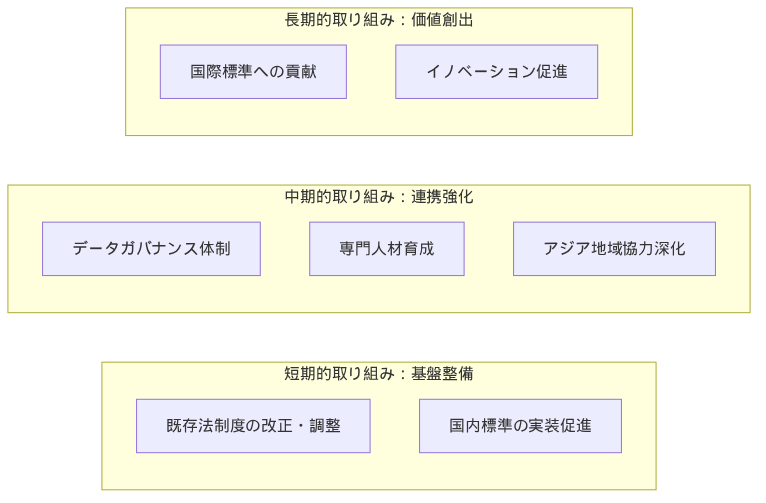
\includegraphics[width=1\linewidth,height=\textheight,keepaspectratio]{images/priority-matrix.png}

}

\caption{日本の医療データ活用推進における優先取組事項}

\end{figure}%

\subsection{1.
短期的取り組み：基盤整備}\label{ux77edux671fux7684ux53d6ux308aux7d44ux307fux57faux76e4ux6574ux5099}

\textbf{事実}：EUは2025年3月に規則を発効し、2027年3月までに実施法令を整備する{[}1{]},
{[}4{]}。日本でも医療データ活用の基盤整備が急務となっている。

\textbf{既存制度の活用と段階的改善}：

\begin{longtable}[]{@{}
  >{\raggedright\arraybackslash}p{(\linewidth - 6\tabcolsep) * \real{0.2381}}
  >{\raggedright\arraybackslash}p{(\linewidth - 6\tabcolsep) * \real{0.1429}}
  >{\raggedright\arraybackslash}p{(\linewidth - 6\tabcolsep) * \real{0.3810}}
  >{\raggedright\arraybackslash}p{(\linewidth - 6\tabcolsep) * \real{0.2381}}@{}}
\toprule\noalign{}
\begin{minipage}[b]{\linewidth}\raggedright
取り組み
\end{minipage} & \begin{minipage}[b]{\linewidth}\raggedright
現状
\end{minipage} & \begin{minipage}[b]{\linewidth}\raggedright
具体的施策例
\end{minipage} & \begin{minipage}[b]{\linewidth}\raggedright
実施主体
\end{minipage} \\
\midrule\noalign{}
\endhead
\bottomrule\noalign{}
\endlastfoot
次世代医療基盤法の活用 &
認定事業者による匿名加工医療情報の利活用{[}93{]} &
オプトアウト通知の電子化・簡素化、認定事業者間のデータ連携基準策定、利活用事例集の公開による認知度向上
& 内閣府・厚労省 \\
個人情報保護法の運用 & 医療分野の特性への配慮が不十分{[}94{]} &
医療データ特有のリスクに対応した実務ガイドライン策定、仮名加工医療情報の具体的な活用シナリオ提示、医療機関向けQ\&A整備
& 個人情報保護委員会 \\
電子カルテ標準化 & HL7 FHIR JP Core策定済み{[}24{]} &
既存システムからFHIR形式への変換ツール無償提供、段階的移行ロードマップ策定、中小医療機関向け導入補助金制度創設
& 厚労省・MEDIS \\
データセキュリティ & 医療機関でのばらつき{[}95{]} &
サイバーセキュリティ成熟度評価ツール開発、地域別セキュリティ支援センター設置、インシデント対応訓練の義務化
& 厚労省・NISC \\
\end{longtable}

\subsection{2.
中期的取り組み：連携強化}\label{ux4e2dux671fux7684ux53d6ux308aux7d44ux307fux9023ux643aux5f37ux5316}

\textbf{考察}：医療データの適切な管理と活用には、ガバナンス体制の構築と専門人材の育成が不可欠である。既存の組織・制度を活用しながら、段階的に体制を強化することが現実的である。

\textbf{データガバナンスと人材育成の推進}：

\begin{longtable}[]{@{}
  >{\raggedright\arraybackslash}p{(\linewidth - 6\tabcolsep) * \real{0.2381}}
  >{\raggedright\arraybackslash}p{(\linewidth - 6\tabcolsep) * \real{0.1429}}
  >{\raggedright\arraybackslash}p{(\linewidth - 6\tabcolsep) * \real{0.3810}}
  >{\raggedright\arraybackslash}p{(\linewidth - 6\tabcolsep) * \real{0.2381}}@{}}
\toprule\noalign{}
\begin{minipage}[b]{\linewidth}\raggedright
取り組み
\end{minipage} & \begin{minipage}[b]{\linewidth}\raggedright
現状
\end{minipage} & \begin{minipage}[b]{\linewidth}\raggedright
具体的施策例
\end{minipage} & \begin{minipage}[b]{\linewidth}\raggedright
実施主体
\end{minipage} \\
\midrule\noalign{}
\endhead
\bottomrule\noalign{}
\endlastfoot
データガバナンス体制 &
データ管理責任者の設置率が低く、利用ポリシーや監査体制が未整備{[}96{]} &
日本版「医療データアクセス機関」設立準備、データ利用審査の統一基準策定、医療機関向けデータガバナンス成熟度モデル導入
& 厚労省・医療団体 \\
専門人材育成 & 先端IT人材が2030年に約54.5万人不足の見込み{[}97{]} &
医療データ分析専門職の育成プログラム開発、医療情報学修士課程の定員拡充、医療機関でのOJT研修制度整備
& 文科省・厚労省 \\
地域医療連携 &
279地域でネットワークが運用、1NWあたり平均143施設が参加{[}98{]} &
地域医療ネットワークの段階的統合、FHIR準拠の共通APIゲートウェイ構築、地域間データ連携実証事業の実施
& 都道府県・厚労省 \\
アジア地域協力 &
PMDAが2019年にAPEC医療機器規制調和の訓練センター（Center of
Excellence）として承認され各国規制当局へ研修提供{[}89{]}、AHWP（アジア医療機器規制調和会議）で医療機器審査基準の標準化を推進{[}92{]}、APEC
Digital Health Roadmap
2030に基づきデジタルヘルス相互運用性を推進{[}99{]} &
ASEANとの医療データ相互運用性パイロット事業開始、アジア版FHIRプロファイル共同開発、PMDA-ATCバンコク事務所での現地研修プログラム拡充
& PMDA・厚労省 \\
データ品質基準 &
ベンダ固有規格により標準規格活用が進まず独自マスター使用が継続{[}100{]}
& ISO/TC
215準拠の日本版医療データ品質基準（JMD-Q）策定、データ品質認証制度の導入、品質監査ツールの開発・配布
& 学会・標準化団体 \\
\end{longtable}

\subsection{3.
長期的取り組み：価値創出}\label{ux9577ux671fux7684ux53d6ux308aux7d44ux307fux4fa1ux5024ux5275ux51fa}

\textbf{考察}：日本の強みである医療機器産業、高齢者医療、災害医療などの分野で蓄積された知見を、国際標準形成に活かしつつ、医療データを活用した新たな価値創出を目指す。

\textbf{国際標準への貢献とイノベーション促進}：

\begin{longtable}[]{@{}
  >{\raggedright\arraybackslash}p{(\linewidth - 6\tabcolsep) * \real{0.2128}}
  >{\raggedright\arraybackslash}p{(\linewidth - 6\tabcolsep) * \real{0.1277}}
  >{\raggedright\arraybackslash}p{(\linewidth - 6\tabcolsep) * \real{0.3404}}
  >{\raggedright\arraybackslash}p{(\linewidth - 6\tabcolsep) * \real{0.3191}}@{}}
\toprule\noalign{}
\begin{minipage}[b]{\linewidth}\raggedright
取り組み
\end{minipage} & \begin{minipage}[b]{\linewidth}\raggedright
現状
\end{minipage} & \begin{minipage}[b]{\linewidth}\raggedright
具体的施策例
\end{minipage} & \begin{minipage}[b]{\linewidth}\raggedright
期待される成果
\end{minipage} \\
\midrule\noalign{}
\endhead
\bottomrule\noalign{}
\endlastfoot
国際標準形成 & IMDRF、ISO等への参画{[}101{]} & ISO/TC
215での医療AI品質評価基準の主導、内視鏡AI診断の国際標準規格提案、継続学習型医療AIの認証フレームワーク策定
& 日本発技術の国際展開促進、年間輸出額1兆円規模 \\
新サービス創出 & 限定的な二次利用{[}93{]} &
医療データ取引市場の創設、製薬企業向けRWD提供プラットフォーム構築、保険会社との健康増進サービス共同開発
& デジタルヘルス産業5兆円市場創出、新規雇用10万人 \\
アジア相互運用 &
医療機器規制ではAHWP等の多国間協力が進む一方{[}92{]}、医療データ相互運用は二国間協力が中心
&
アジア健康データ空間（AHDS）の構築、APEC加盟国での相互運用性フレームワーク確立、越境診療・処方の段階的実現
& アジア太平洋地域の医療データ市場形成、日本企業の市場アクセス確保 \\
高齢社会ソリューション &
介護保険制度{[}69{]}、認知症対策{[}70{]}、地域包括ケア{[}71{]}等の国内実績
&
認知症ケア・介護ロボット・遠隔見守りの統合パッケージ輸出、ASEAN各国での高齢者ケアセンター展開、介護人材育成プログラムの国際展開
& アジア高齢者ケア市場でのシェア獲得、関連ソリューション輸出拡大 \\
研究開発促進 &
次世代医療基盤法の認定事業者経由での限定的なデータアクセス{[}93{]} &
大規模統合医療データベース構築、AI創薬プラットフォームの商用化、希少疾患研究の国際コンソーシアム主導
& 新薬開発期間の短縮、開発コスト削減、新薬候補創出の加速 \\
\end{longtable}

\begin{tcolorbox}[enhanced jigsaw, toprule=.15mm, bottomtitle=1mm, coltitle=black, left=2mm, opacityback=0, arc=.35mm, colbacktitle=quarto-callout-note-color!10!white, colback=white, opacitybacktitle=0.6, bottomrule=.15mm, rightrule=.15mm, breakable, title=\textcolor{quarto-callout-note-color}{\faInfo}\hspace{0.5em}{Note}, toptitle=1mm, titlerule=0mm, colframe=quarto-callout-note-color-frame, leftrule=.75mm]

\textbf{段階的実施の重要性}：上記の取り組みは、短期（基盤整備）・中期（連携強化）・長期（価値創出）の3段階で段階的に実施することが重要である。急激な変革を避け、既存システムとの共存を図りながら、確実な成果を積み重ねていく漸進的アプローチが、日本の医療データ活用推進において最も現実的な道筋である。

一方で、EHDSが2029年に本格稼働し、米国TEFCAも2024年から実装が進む中、日本が国際競争力を維持するためには、「慎重さ」と「迅速性」のバランスが不可欠である。段階的実施を言い訳とした先送りではなく、明確な期限設定と実行責任の所在を定めた上で、確実な推進力を持って取り組むことが求められる。

\end{tcolorbox}

\section{投資規模の試算}\label{ux6295ux8cc7ux898fux6a21ux306eux8a66ux7b97}

\subsection{必要投資額（5年間）}\label{ux5fc5ux8981ux6295ux8cc7ux984d5ux5e74ux9593}

\textbf{事実}：EUはデジタルヘルス・EHDS関連で複数の資金枠組みを設定している。

EU4Healthプログラムについて、欧州委員会は以下のように述べている：
\textgreater{} ``with an initial €5.3 billion budget for the 2021-27
period, reduced to €4.4 billion following the revision of the 2021-2027
MFF''（2021-27年期間の当初予算53億ユーロは、2021-2027年多年度財政枠組み（MFF）の見直しにより44億ユーロに削減）{[}102{]}

EHDS実装について、欧州委員会は以下のように明記している： \textgreater{}
``The Commission will provide over €810 million: €280 million under the
EU4Health Programme and the rest via the Digital Europe Programme,
Connecting Europe Facility and Horizon
Europe''（欧州委員会は8.1億ユーロ以上を提供：EU4Healthプログラムから2.8億ユーロ、残りはDigital
Europe Programme、Connecting Europe Facility、Horizon
Europeから）{[}103{]}

さらに、復興レジリエンス基金（Recovery and Resilience Facility:
RRF）について、欧州委員会は以下のように報告している： \textgreater{}
``Member States have budgeted €14 billion for investments in digital
health under the Recovery and Resilience Facility
(RRF)''（加盟国は復興レジリエンス基金（RRF）の下でデジタルヘルスへの投資に140億ユーロを予算化している）{[}104{]}

RRFは、COVID-19パンデミックからの経済復興を支援するためのEUの一時的な資金提供メカニズムで、NextGenerationEUの中核をなすものである。この基金は、経済をより持続可能で、強靭で、グリーン・デジタル移行に対応できるようにすることを目的としている。

\textbf{参考：EUの投資規模との比較検討}：

\begin{enumerate}
\def\labelenumi{\arabic{enumi}.}
\tightlist
\item
  \textbf{EUのデジタルヘルス関連投資総額（概算）}：

  \begin{itemize}
  \tightlist
  \item
    EU4Health: 44億ユーロ（約6,600億円、1ユーロ=150円換算）
  \item
    EHDS直接投資: 8.1億ユーロ（約1,215億円）
  \item
    RRFデジタルヘルス: 140億ユーロ（約2兆1,000億円）
  \item
    \textbf{合計: 約192億ユーロ（約2兆8,800億円）}
  \end{itemize}
\item
  \textbf{GDP比での調整}：

  \begin{itemize}
  \tightlist
  \item
    EU GDP: 約16.6兆ドル（2023年）{[}105{]}
  \item
    日本GDP: 約4.2兆ドル（2023年）{[}106{]}
  \item
    \textbf{GDP比: 日本/EU ≈ 0.25（約1/4）}
  \end{itemize}
\item
  \textbf{日本における現実的な投資規模の検討}：

  \begin{itemize}
  \tightlist
  \item
    GDP比での単純計算では2兆8,800億円 × 0.25 =
    約7,200億円となるが、これは機械的な試算
  \item
    \textbf{より現実的な投資規模として、5年間で約2,590億円（年間約518億円）を提案}

    \begin{itemize}
    \tightlist
    \item
      既存システムの相互接続・標準化：約1,490億円
    \item
      セキュリティ強化・プライバシー保護：約400億円\\
    \item
      人材育成・組織体制整備：約700億円
    \end{itemize}
  \item
    この規模は、既存インフラを最大限活用し、段階的導入により初期投資を抑制した試算
  \item
    日本の投資規模を検討する際の考慮事項：

    \begin{itemize}
    \tightlist
    \item
      EUは27カ国の異なるシステムを統合する必要があるのに対し、日本は単一国家
    \item
      日本は既にNDB（レセプトDB）、介護DB、DPCデータベース等の全国規模データベースが稼働中
    \item
      電子カルテ普及率は病院で91.2\%、診療所で49.9\%（2020年）{[}107{]}
    \item
      マイナンバーカードを活用した医療情報連携基盤が整備途上
    \end{itemize}
  \item
    EUとの比較から見た日本の優位性：

    \begin{itemize}
    \tightlist
    \item
      \textbf{システム統合の効率性}: EUは27カ国分の統合コスト →
      日本は単一国家で効率的
    \item
      \textbf{言語・制度の統一}: EUは24言語対応が必要 → 日本は単一言語
    \item
      \textbf{既存インフラ活用}: EUは新規構築 →
      日本は既存システムの改修・接続が中心
    \end{itemize}
  \end{itemize}
\end{enumerate}

\subsubsection{6.3.1.1
投資内訳の詳細}\label{ux6295ux8cc7ux5185ux8a33ux306eux8a73ux7d30}

\begin{tcolorbox}[enhanced jigsaw, toprule=.15mm, bottomtitle=1mm, coltitle=black, left=2mm, opacityback=0, arc=.35mm, colbacktitle=quarto-callout-note-color!10!white, colback=white, opacitybacktitle=0.6, bottomrule=.15mm, rightrule=.15mm, breakable, title=\textcolor{quarto-callout-note-color}{\faInfo}\hspace{0.5em}{Note}, toptitle=1mm, titlerule=0mm, colframe=quarto-callout-note-color-frame, leftrule=.75mm]

\textbf{日本の医療データ基盤整備投資内訳}

\begin{enumerate}
\def\labelenumi{\arabic{enumi}.}
\tightlist
\item
  \textbf{既存システムの相互接続・標準化（約1,490億円）}：

  \begin{itemize}
  \tightlist
  \item
    医療機関のシステム改修{[}108{]}

    \begin{itemize}
    \tightlist
    \item
      病院（約8,100施設）：厚労省の電子カルテ情報共有サービス接続改修事業における標準的な改修費用{[}109{]}

      \begin{itemize}
      \tightlist
      \item
        健診実施医療機関：200床以上1,316万円、200床未満1,091万円（事業額上限、補助率50\%）
      \item
        健診未実施医療機関：200床以上1,016万円、200床未満817万円（事業額上限、補助率50\%）
      \item
        推定改修費用：1施設あたり平均1,200万円 × 8,100施設 = 約972億円
      \end{itemize}
    \item
      診療所（約10.5万施設）：クラウド型への移行やAPI接続対応

      \begin{itemize}
      \tightlist
      \item
        推定改修費用：1施設あたり平均100万円 × 10.5万施設 = 約1,050億円
      \item
        ただし、多くの診療所は段階的導入のため、初期は約30\%（3.5万施設）が対応と想定
        = 約350億円
      \end{itemize}
    \end{itemize}
  \item
    地域医療連携ネットワーク（279地域）の相互接続・標準化：約150億円

    \begin{itemize}
    \tightlist
    \item
      日本医師会総合政策研究機構の2023年度調査によると、279地域でネットワークが運用中{[}110{]}
    \item
      同調査では、1ネットワークあたりの平均構築費用（累計）は2億5,409万1千円、2024年度の平均年間運営予算は1,185万円と報告されている{[}110{]}
    \item
      相互接続・標準化対応改修：既存システム構築費用の約20\%程度と想定（平均構築費用2.54億円の20\%
      = 約5,000万円/地域）× 279地域 = 約140億円
    \end{itemize}
  \item
    データ変換・移行支援、研修・技術支援等：約28億円

    \begin{itemize}
    \tightlist
    \item
      \textbf{データ変換ツール開発・提供（約10億円）}：

      \begin{itemize}
      \tightlist
      \item
        \textbf{開発フェーズ（約4億円）}：

        \begin{itemize}
        \tightlist
        \item
          HL7 v2→FHIR変換エンジン開発：1.5億円（主要10パターン対応）
        \item
          SS-MIX2→FHIR変換モジュール：1億円
        \item
          各ベンダー（主要20社）向けアダプター開発：1億円（500万円×20社）
        \item
          テストツール・SDK・ドキュメント整備：0.5億円
        \end{itemize}
      \item
        \textbf{導入支援フェーズ（約3億円）}：

        \begin{itemize}
        \tightlist
        \item
          パイロット病院での実証実験（20施設）：1億円
        \item
          各ベンダーへの技術移転・研修：1億円
        \item
          導入コンサルティング・問い合わせ対応体制：1億円
        \end{itemize}
      \item
        \textbf{保守・運用フェーズ（約3億円）}：

        \begin{itemize}
        \tightlist
        \item
          5年間の保守・アップデート：年間6,000万円×5年
        \end{itemize}
      \item
        参考：厚労省の「電子カルテ情報共有サービス」等の全国共通基盤開発では数億円規模の投資が一般的
      \end{itemize}
    \item
      \textbf{医療従事者向け研修プログラム（全国展開：約8億円）}：

      \begin{itemize}
      \tightlist
      \item
        東京都医療機関デジタル化推進セミナーのような研修を全国展開{[}111{]}
      \item
        全国約8,100病院×研修費10万円（基礎編・実践編）= 約8.1億円
      \item
        オンライン研修プラットフォーム構築・運用費を含む
      \item
        参考：令和6年度補正予算では介護人材確保・職場環境改善等事業に806億円が計上{[}112{]}
      \end{itemize}
    \item
      \textbf{技術支援センター設置・運営（5年間：約10億円）}：

      \begin{itemize}
      \tightlist
      \item
        全国5ブロック（北海道・東北、関東、中部、関西、中国・四国・九州）に設置
      \item
        各センター年間運営費：4,000万円（人件費3名＋運営費）× 5拠点 =
        2億円/年
      \item
        5年間の総額：2億円 × 5年 = 10億円
      \item
        参考：PMDAアジア医薬品・医療機器研修センター（PMDA-ATC）の運営実績{[}89{]}
      \end{itemize}
    \end{itemize}
  \end{itemize}
\item
  \textbf{セキュリティ強化・プライバシー保護（5年間で約400億円）}：

  \begin{itemize}
  \tightlist
  \item
    \textbf{サイバーセキュリティ対策強化（約200億円）}：

    \begin{itemize}
    \tightlist
    \item
      厚労省「医療機関におけるサイバーセキュリティ確保事業」：110億円（2024-2025年度予算）{[}113{]}
    \item
      対象：電子カルテ導入済み20床以上の病院（約2,000施設）
    \item
      外部ネットワーク接続の安全性検証、オフラインバックアップシステム構築
    \item
      追加的なセキュリティ投資（民間負担分）：90億円
    \end{itemize}
  \item
    \textbf{段階的なゼロトラスト環境への移行（約100億円）}{[}114{]}：

    \begin{itemize}
    \tightlist
    \item
      重点病院（500施設）への先行導入：50億円
    \item
      ID管理・認証、EDR、CASB等の段階的実装
    \item
      中小医療機関向けクラウド型セキュリティサービス：50億円
    \end{itemize}
  \item
    \textbf{医療データ暗号化・匿名化技術の標準化（約100億円）}{[}115{]}：

    \begin{itemize}
    \tightlist
    \item
      次世代医療基盤法認定事業者の技術開発支援：30億円
    \item
      匿名加工・仮名加工処理技術の標準化：30億円
    \item
      全国展開のためのシステム実装・保守：40億円
    \end{itemize}
  \end{itemize}
\item
  \textbf{人材育成・組織体制整備（約700億円）}：

  \begin{itemize}
  \tightlist
  \item
    \textbf{医療データ分析専門人材育成（約400億円）}：

    \begin{itemize}
    \tightlist
    \item
      既存の医療情報技師（約2.7万人認定）\textbf{JAMI2024?}の高度化研修：1人あたり50万円
      × 1万人 = 50億円
    \item
      新規人材育成（データサイエンティスト養成）：

      \begin{itemize}
      \tightlist
      \item
        第四次産業革命スキル習得講座（経産省認定）等の活用{[}116{]}
      \item
        専門実践教育訓練給付金による受講費用の50-80\%補助を前提
      \item
        実質負担額：1人あたり年間100万円 × 5年間 × 5,000人 = 250億円
      \end{itemize}
    \item
      大学・大学院での専門コース設置支援：100億円（20大学 × 5億円）
    \end{itemize}
  \item
    \textbf{医療機関のデジタル人材配置支援（約200億円）}：

    \begin{itemize}
    \tightlist
    \item
      病院（8,100施設）への配置支援：1施設あたり200万円/年 × 5年 ×
      2,000施設（重点病院）= 200億円
    \item
      診療所向けは既存のIT導入補助金制度を活用
    \end{itemize}
  \item
    \textbf{データガバナンス体制構築支援（約100億円）}：

    \begin{itemize}
    \tightlist
    \item
      ガイドライン策定・普及：10億円
    \item
      医療機関向けガバナンス研修：50億円（全病院対象）
    \item
      データ管理責任者（CDO）認定制度構築・運営：40億円
    \end{itemize}
  \end{itemize}
\end{enumerate}

\end{tcolorbox}

\subsubsection{6.3.1.2
投資配分と実施計画}\label{ux6295ux8cc7ux914dux5206ux3068ux5b9fux65bdux8a08ux753b}

\textbf{投資配分案}：

\begin{figure}[H]

{\centering \pandocbounded{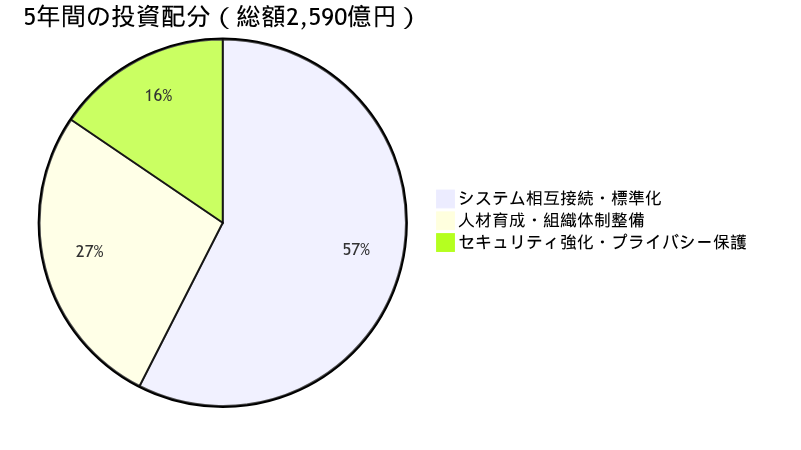
\includegraphics[keepaspectratio]{images/investment-allocation.png}}

}

\caption{5年間の投資配分}

\end{figure}%

\begin{longtable}[]{@{}lll@{}}
\toprule\noalign{}
カテゴリー & 投資額（億円） & 割合 \\
\midrule\noalign{}
\endhead
\bottomrule\noalign{}
\endlastfoot
システム相互接続・標準化 & 1,490 & 57.5\% \\
人材育成・組織体制整備 & 700 & 27.0\% \\
セキュリティ強化・プライバシー保護 & 400 & 15.5\% \\
\textbf{合計} & \textbf{2,590} & \textbf{100\%} \\
\end{longtable}

\subsection{ROI（投資対効果）予測}\label{roiux6295ux8cc7ux5bfeux52b9ux679cux4e88ux6e2c}

\begin{tcolorbox}[enhanced jigsaw, toprule=.15mm, bottomtitle=1mm, coltitle=black, left=2mm, opacityback=0, arc=.35mm, colbacktitle=quarto-callout-warning-color!10!white, colback=white, opacitybacktitle=0.6, bottomrule=.15mm, rightrule=.15mm, breakable, title=\textcolor{quarto-callout-warning-color}{\faExclamationTriangle}\hspace{0.5em}{Warning}, toptitle=1mm, titlerule=0mm, colframe=quarto-callout-warning-color-frame, leftrule=.75mm]

\textbf{野心的目標設定の重要性}：
以下に示すROI予測は、国内外の先進事例とエビデンスに基づく「期待効果」である。これらは自動的に実現される成果ではなく、官民が一体となって戦略的に追求すべき目標値として位置づけるべきである。特に、デジタル化の恩恵を最大化するには、単なるシステム導入を超えて、業務プロセスの根本的な変革と、データ活用による新たな価値創造への積極的な取り組みが不可欠である。

\end{tcolorbox}

EHDS参考による医療データ基盤構築の日本における期待効果は、\textbf{年間総額1.3兆円〜1.9兆円}と試算される。ただし、この試算には医療DX推進全般の効果が含まれており、データ基盤固有の効果はこの一部である。投資額2,590億円は5年間の段階的投資を想定しており、効果の完全実現には7-10年程度を要すると考えられる。期待される効果は以下の5つの分野に分類される：

\subsubsection{1.
医療費削減効果（年間5,000億円〜8,600億円）}\label{ux533bux7642ux8cbbux524aux6e1bux52b9ux679cux5e74ux95935000ux5104ux51868600ux5104ux5186}

\textbf{1.1 重複検査の削減（年間1,600億円〜3,200億円）}

\emph{※この効果はEHDS型データ基盤の中核機能である医療機関間情報共有により直接実現}

厚生労働省は医療DXの効果について以下のように指摘している：

\begin{quote}
「医療機関間での情報共有により、重複検査の削減が期待される。電子カルテ情報共有サービスの活用により、患者の検査履歴・投薬履歴を医療機関間で共有することで、医療の質向上と効率化を実現する」{[}117{]}
\end{quote}

\textbf{算出根拠}：

\begin{itemize}
\tightlist
\item
  医療費全体（約47兆円）に占める検査・画像診断の割合：約8-10\%（推計3.8〜4.7兆円）\footnote{この推計は、社会医療診療行為別統計において入院患者の画像診断が日割り点数の1.0\%、検査が2.0\%を占めること{[}118{]}や、日本のCT・MRI設置密度が世界最高水準であること{[}108{]}を総合的に勘案した概算値である。より詳細な費用構造分析には、診療行為別の詳細な費用調査が必要である。}
\end{itemize}

\begin{itemize}
\tightlist
\item
  複数医療機関受診による重複検査の発生：医療機関間の情報共有不足により発生\footnote{厚生労働省の医療費適正化政策において、重複受診・重複検査は医療費増加要因として指摘されているが、全国レベルでの発生率を示す公的統計は限定的である。地域の健康保険組合等では重複受診対策が実施されており、情報共有による削減効果が期待されている。}
\end{itemize}

\begin{itemize}
\tightlist
\item
  情報共有による重複検査削減可能率：80\%と仮定
\end{itemize}

\textbf{算出式}：

\begin{verbatim}
削減額 = 検査関連医療費 × 重複検査発生率 × 削減可能率
      = 4兆円 × 5〜10% × 80%
      = 1,600億円〜3,200億円/年
\end{verbatim}

\textbf{1.2 予防医療・重症化予防（年間3,400億円〜5,400億円）}

経済産業省は健康経営の効果について具体的な数値を示している：

\begin{quote}
「健康経営に取り組む企業では、従業員一人当たりの医療費が平均的に10\%程度削減される傾向が見られる。また、プレゼンティーイズム（健康問題による生産性低下）の改善により、労働生産性が向上する」{[}119{]}
\end{quote}

\textbf{算出根拠}：

\begin{itemize}
\tightlist
\item
  生活習慣病関連医療費：約10兆円（医療費全体の約20\%）
\item
  糖尿病患者数：約1,000万人、透析患者数：約35万人
\item
  人工透析医療費：1人あたり年間約500万円
\item
  重症化予防プログラムによる透析移行抑制率：20-30\%と仮定
\end{itemize}

\textbf{算出式}：

\begin{verbatim}
削減額 = (生活習慣病医療費 × 予防効果率) + (透析新規導入抑制による削減)
      = (10兆円 × 3〜5%) + (4万人/年 × 500万円 × 20%)
      = 3,000億円〜5,000億円 + 400億円
      = 3,400億円〜5,400億円/年
\end{verbatim}

\subsubsection{2.
業務効率化効果（年間2,200億円〜4,400億円）}\label{ux696dux52d9ux52b9ux7387ux5316ux52b9ux679cux5e74ux95932200ux5104ux51864400ux5104ux5186}

\textbf{2.1 事務作業の削減（年間1,000億円〜2,000億円）}

厚生労働省の医療経済実態調査によると、一般病院における給与費は医業・介護収益の約57\%を占めており{[}120{]}、医療従事者の事務作業負担軽減によるコスト削減効果は大きい。

\textbf{算出根拠}：

\begin{itemize}
\tightlist
\item
  国民医療費（2022年度：46.7兆円）{[}121{]}のうち、医療機関の費用構造では人件費が最大の割合を占める
\item
  医療従事者の事務作業負担は広く認識されている課題であり、医師事務作業補助者の配置やタスクシフト/シェアが政策的に推進されている
\item
  デジタル化による期待効果：電子カルテの完全普及、レセプト電子化、オンライン資格確認システムなどの導入により、事務作業の効率化が期待される
\end{itemize}

医療DX推進により、医療従事者の業務効率改善を通じて費用削減が期待される。医療機関の費用構造において人件費が大きな割合を占めることから、業務効率化の影響は大きい。ただし、具体的な人件費総額のデータが明確でないため、保守的に見積もり：

\begin{itemize}
\tightlist
\item
  推定削減額：1,000億円〜2,000億円/年
\end{itemize}

\textbf{2.2 AI活用による診断支援（年間1,200億円〜2,400億円）}

AI診断支援システムの導入により、診断時間の短縮と精度向上が期待される。

\textbf{算出根拠}：

\begin{itemize}
\tightlist
\item
  画像診断関連医療費：約2兆円/年（推計）
\item
  放射線科医・病理医等の専門医不足による診断遅延コスト
\item
  AI導入による診断時間短縮率：30-50\%
\item
  診断精度向上による不要な再検査削減率：10-20\%と仮定
\end{itemize}

\textbf{算出式}：

\begin{verbatim}
削減額 = (画像診断費 × 効率化率) + (再検査削減による効果)
      = (2兆円 × 5〜10%) + (2兆円 × 10% × 10〜20%)
      = 1,000億円〜2,000億円 + 200億円〜400億円
      = 1,200億円〜2,400億円/年
\end{verbatim}

\subsubsection{3.
新産業創出効果（年間5,000億円）}\label{ux65b0ux7523ux696dux5275ux51faux52b9ux679cux5e74ux95935000ux5104ux5186}

\textbf{3.1 デジタルヘルス市場の成長}

\emph{※新産業創出効果の一部は医療DX全般、一部はデータ基盤活用による直接効果}

富士経済の調査によると、医療DX推進により多岐にわたる市場成長が期待される{[}122{]}：

\textbf{既存市場の拡大}：

\begin{itemize}
\tightlist
\item
  電子カルテ・PHR市場：2,425億円（2030年予測）
\item
  リアルワールドデータ分析市場：320億円（2030年予測）
\end{itemize}

\textbf{新規市場創出}：

\begin{itemize}
\tightlist
\item
  AI診断支援システム市場：約1,000億円（推計、海外事例より）
\item
  遠隔医療・オンライン診療市場：約500億円（推計）
\item
  ウェアラブルデバイス・健康管理アプリ市場：約800億円（推計）
\end{itemize}

\textbf{創薬支援効果}（国内製薬業界研究開発費：年間約2兆円）：

\begin{itemize}
\tightlist
\item
  開発期間短縮（2-3年）による機会コスト削減：約20-30\%
\item
  臨床試験の効率化による開発コスト削減：約20-30\%
\item
  成功確率向上による無駄な開発の削減：約10-15\%
\end{itemize}

\textbf{算出式}：

\begin{verbatim}
新産業創出総額 = 既存市場拡大 + 新規市場創出 + 創薬効率化効果の一部
               = (2,425億円 + 320億円) + (1,000億円 + 500億円 + 800億円) + α
               = 2,745億円 + 2,300億円 + α
               ≈ 5,000億円/年
\end{verbatim}

\subsubsection{4.
輸出産業化効果（年間1,000億円〜1,500億円）}\label{ux8f38ux51faux7523ux696dux5316ux52b9ux679cux5e74ux95931000ux5104ux51861500ux5104ux5186}

\textbf{4.1 アジア太平洋市場への展開}

日本の医療技術の競争優位（内視鏡70\%シェア、画像診断装置等）を活かし、デジタルソリューション付加価値による輸出拡大が期待される。

\textbf{算出根拠}：

\begin{itemize}
\tightlist
\item
  アジア太平洋デジタルヘルス市場規模：2030年に2,520億ドル（約37兆円）{[}61{]}
\item
  現在の日本の医療機器輸出額：約8,000億円/年（2022年実績）\textbf{METI2023Medical?}
\item
  日本の競争優位分野：内視鏡（世界シェア約70\%）、画像診断装置（CT/MRI）、高齢者ケアソリューション、医療データ分析・AI診断支援
\end{itemize}

\textbf{算出式}：

\begin{verbatim}
推定輸出額 = 市場規模 × 獲得可能シェア率
          = 37兆円 × 0.3〜0.5%（保守的推計）
          = 1,110億円〜1,850億円/年

または

推定輸出額 = 既存医療機器輸出 × デジタル化による増加率
          = 8,000億円 × 12.5〜18.75%（デジタルソリューション付加価値）
          = 1,000億円〜1,500億円/年
\end{verbatim}

\begin{itemize}
\tightlist
\item
  推定輸出額：1,000億円〜1,500億円/年（2030年）
\end{itemize}

\subsubsection{5.
健康経営効果（参考事例）}\label{ux5065ux5eb7ux7d4cux55b6ux52b9ux679cux53c2ux8003ux4e8bux4f8b}

ジョンソン・エンド・ジョンソンの健康経営プログラムは世界的な成功事例として知られている：

\begin{quote}
「私たちのWellness \& Prevention
プログラムへの投資は、1ドルあたり3ドルのリターンを生み出しています。これは医療費の削減、欠勤率の低下、生産性の向上を通じて実現されています」{[}123{]}
\end{quote}

国内企業でも従業員の病欠が年20\%減少、医療費負担が10\%削減の実績がある。

\subsubsection{ROI総合評価}\label{roiux7dcfux5408ux8a55ux4fa1}

\begin{longtable}[]{@{}
  >{\raggedright\arraybackslash}p{(\linewidth - 4\tabcolsep) * \real{0.2703}}
  >{\raggedright\arraybackslash}p{(\linewidth - 4\tabcolsep) * \real{0.2973}}
  >{\raggedright\arraybackslash}p{(\linewidth - 4\tabcolsep) * \real{0.4324}}@{}}
\toprule\noalign{}
\begin{minipage}[b]{\linewidth}\raggedright
効果分野
\end{minipage} & \begin{minipage}[b]{\linewidth}\raggedright
年間効果額
\end{minipage} & \begin{minipage}[b]{\linewidth}\raggedright
主要な算出根拠
\end{minipage} \\
\midrule\noalign{}
\endhead
\bottomrule\noalign{}
\endlastfoot
\textbf{1. 医療費削減} & \textbf{5,000〜8,600億円} & \\
├ 重複検査削減 & 1,600〜3,200億円 &
検査費4兆円×重複率5-10\%×削減率80\% \\
└ 予防医療・重症化予防 & 3,400〜5,400億円 &
生活習慣病10兆円×予防効果3-5\%+透析抑制400億円 \\
\textbf{2. 業務効率化} & \textbf{2,200〜4,400億円} & \\
├ 事務作業削減 & 1,000〜2,000億円 &
医療DXによる業務効率改善（保守的推計） \\
└ AI診断支援 & 1,200〜2,400億円 &
画像診断2兆円×効率化5-10\%+再検査削減 \\
\textbf{3. 新産業創出} & \textbf{5,000億円} &
既存市場拡大2,745億円+新規市場創出2,300億円 \\
\textbf{4. 輸出産業化} & \textbf{1,000〜1,500億円} &
アジア太平洋市場37兆円×獲得シェア0.3-0.5\% \\
\textbf{年間効果総額} & \textbf{1.3兆円〜1.9兆円} &
\textbf{投資額2,590億円（5年間）} \\
\textbf{長期的ROI} & \textbf{500〜733\%} &
\textbf{完全実現時（7-10年後）の年間効果対累積投資比} \\
\end{longtable}

\begin{tcolorbox}[enhanced jigsaw, toprule=.15mm, bottomtitle=1mm, coltitle=black, left=2mm, opacityback=0, arc=.35mm, colbacktitle=quarto-callout-note-color!10!white, colback=white, opacitybacktitle=0.6, bottomrule=.15mm, rightrule=.15mm, breakable, title=\textcolor{quarto-callout-note-color}{\faInfo}\hspace{0.5em}{Note}, toptitle=1mm, titlerule=0mm, colframe=quarto-callout-note-color-frame, leftrule=.75mm]

\textbf{段階的な効果発現とリアルな投資回収}：

\textbf{効果発現スケジュール}：

\begin{itemize}
\tightlist
\item
  初期段階：基盤構築期（効果10-20\%）
\item
  拡大段階：普及促進期（効果30-60\%）
\item
  成熟段階：本格活用期（効果70-90\%）
\item
  完全実現段階：システム成熟期（効果100\%）
\end{itemize}

\textbf{投資回収の現実的見通し}：

\begin{itemize}
\tightlist
\item
  投資額2,590億円を段階的に実施
\item
  継続的な投資に対し、段階的に効果が発現
\item
  実質的な投資回収は中長期的に実現
\item
  効果の完全実現には、全医療機関での標準化、医療従事者のデジタルリテラシー向上、制度整備が前提
\end{itemize}

\textbf{リスク要因}：技術標準の変化、医療機関の導入遅延、人材不足、制度変更等により効果発現が遅れる可能性がある。

\end{tcolorbox}

\section{リスク管理戦略}\label{ux30eaux30b9ux30afux7ba1ux7406ux6226ux7565}

\subsection{主要リスクと対策}\label{ux4e3bux8981ux30eaux30b9ux30afux3068ux5bfeux7b56}

\begin{tcolorbox}[enhanced jigsaw, toprule=.15mm, bottomtitle=1mm, coltitle=black, left=2mm, opacityback=0, arc=.35mm, colbacktitle=quarto-callout-important-color!10!white, colback=white, opacitybacktitle=0.6, bottomrule=.15mm, rightrule=.15mm, breakable, title=\textcolor{quarto-callout-important-color}{\faExclamation}\hspace{0.5em}{Important}, toptitle=1mm, titlerule=0mm, colframe=quarto-callout-important-color-frame, leftrule=.75mm]

\textbf{重大リスクの認識}：
医療データ基盤整備は、技術的課題だけでなく、社会的受容性、現場の協力、法制度の整備など、多面的なリスク管理が不可欠である。特に以下の3つは、プロジェクト全体を頓挫させる可能性がある：

\begin{enumerate}
\def\labelenumi{\arabic{enumi}.}
\tightlist
\item
  \textbf{個人情報漏洩による信頼失墜} -
  一度の重大インシデントで国民の信頼を完全に失う
\item
  \textbf{医療現場の抵抗・変革疲労} -
  現場の協力なくしては、どんなシステムも機能しない
\item
  \textbf{ベンダーロックインによる硬直化} -
  特定企業への依存は、長期的な発展を阻害する
\end{enumerate}

\end{tcolorbox}

\textbf{包括的リスクマトリクス}：

\begin{longtable}[]{@{}
  >{\raggedright\arraybackslash}p{(\linewidth - 10\tabcolsep) * \real{0.2069}}
  >{\raggedright\arraybackslash}p{(\linewidth - 10\tabcolsep) * \real{0.2069}}
  >{\raggedright\arraybackslash}p{(\linewidth - 10\tabcolsep) * \real{0.1724}}
  >{\raggedright\arraybackslash}p{(\linewidth - 10\tabcolsep) * \real{0.1379}}
  >{\raggedright\arraybackslash}p{(\linewidth - 10\tabcolsep) * \real{0.1034}}
  >{\raggedright\arraybackslash}p{(\linewidth - 10\tabcolsep) * \real{0.1724}}@{}}
\toprule\noalign{}
\begin{minipage}[b]{\linewidth}\raggedright
リスク分類
\end{minipage} & \begin{minipage}[b]{\linewidth}\raggedright
リスク内容
\end{minipage} & \begin{minipage}[b]{\linewidth}\raggedright
発生確率
\end{minipage} & \begin{minipage}[b]{\linewidth}\raggedright
影響度
\end{minipage} & \begin{minipage}[b]{\linewidth}\raggedright
対策
\end{minipage} & \begin{minipage}[b]{\linewidth}\raggedright
責任主体
\end{minipage} \\
\midrule\noalign{}
\endhead
\bottomrule\noalign{}
\endlastfoot
\textbf{セキュリティ} & サイバー攻撃・情報漏洩 & 高 & 極大 &
ゼロトラスト、SOC設置、継続的監査 & デジタル庁 \\
\textbf{社会的受容} & 市民の反対・理解不足 & 中 & 大 &
段階的導入、透明性確保、成功事例の可視化 & 厚労省 \\
\textbf{現場対応} & 医療従事者の抵抗・変革疲労 & 高 & 極大 &
業務負担軽減の実証、段階的移行、インセンティブ設計 & 厚労省・医師会 \\
\textbf{技術的課題} & システム障害・相互運用性欠如 & 中 & 大 &
アジャイル開発、MVP、標準化徹底 & IT企業・MEDIS \\
\textbf{ベンダー依存} & ロックイン・技術的分断 & 高 & 大 &
オープンスタンダード義務化、マルチベンダー環境 & デジタル庁・公取委 \\
\textbf{法制度} & 規制の硬直性・省庁縦割り & 高 & 大 &
規制サンドボックス、省庁横断タスクフォース & 内閣府 \\
\textbf{財政} & 予算不足・費用超過 & 中 & 中 &
官民連携、段階投資、効果測定 & 財務省 \\
\textbf{地域格差} & デジタルディバイド拡大 & 中 & 大 &
地方優先投資、クラウド型サービス & 総務省 \\
\textbf{国際競争} & 標準化競争での劣後 & 高 & 大 &
早期着手、AHDS主導、標準準拠 & 経産省 \\
\textbf{投資効果} & ROI未達成・便益過大評価 & 中 & 極大 &
KPI設定、段階的効果測定、外部評価 & 会計検査院 \\
\end{longtable}

\begin{tcolorbox}[enhanced jigsaw, toprule=.15mm, bottomtitle=1mm, coltitle=black, left=2mm, opacityback=0, arc=.35mm, colbacktitle=quarto-callout-note-color!10!white, colback=white, opacitybacktitle=0.6, bottomrule=.15mm, rightrule=.15mm, breakable, title=\textcolor{quarto-callout-note-color}{\faInfo}\hspace{0.5em}{Note}, toptitle=1mm, titlerule=0mm, colframe=quarto-callout-note-color-frame, leftrule=.75mm]

\textbf{リスク評価の根拠と考察}：

上記の発生確率評価は、以下の実績データと動向分析に基づく：

\textbf{「高」確率と評価した根拠}：

\begin{itemize}
\tightlist
\item
  \textbf{サイバー攻撃}:
  2021年以降、医療機関へのランサムウェア攻撃が急増。日本では徳島県つるぎ町立半田病院（2021年10月）、大阪急性期・総合医療センター（2022年10月）等で電子カルテシステムが長期間停止する重大事例が発生{[}124{]}
\item
  \textbf{医療現場の抵抗}:
  オンライン資格確認システム導入時の混乱（2021-2023年）、診療所の電子カルテ普及率が49.9\%に留まる現状{[}107{]}
\item
  \textbf{ベンダーロックイン}:
  電子カルテ市場は上位5社で70\%以上のシェアを占め、ベンダー独自仕様が標準化を阻害{[}125{]}
\item
  \textbf{法制度の硬直性}:
  次世代医療基盤法の認定事業者は7社に留まり、活用が限定的{[}93{]}
\end{itemize}

\textbf{「中」確率と評価した根拠}：

\begin{itemize}
\tightlist
\item
  \textbf{市民の反対}:
  マイナンバーカード保有率75\%に達するも、デジタル化に対し「良いと思わない」11.1\%、「どちらともいえない」38.0\%の慎重論が存在。医療データ連携への不安は別途調査が必要{[}126{]}
\item
  \textbf{地域格差}:
  医療情報技師能力検定試験は全国13箇所で実施されるが、IT人材・医療従事者の地域偏在により実装格差が生じる可能性{[}127{]}
\item
  \textbf{投資効果}:
  政府情報システムに関する会計検査で、縦割りによる重複投資、個別最適化による非効率、予算要求段階での軌道修正困難などの構造的課題が指摘されている{[}128{]}
\end{itemize}

\textbf{技術的課題を「低」から「中」に再評価した根拠}：

当初「低」としていたが、日本の大規模IT
プロジェクトの実績を踏まえ「中」に修正：

\begin{itemize}
\tightlist
\item
  \textbf{大規模システム開発の課題}:
  政府情報システムでは縦割りによる重複投資、個別最適による非効率、人材不足による品質・コスト両立の困難などの構造的課題が存在{[}128{]}。年金記録システム（2017年刷新、約3,000億円投資）、マイナンバーシステム（2016年開始、複数の障害発生）等の事例もある
\item
  \textbf{医療系システムの複雑性}:
  既存の電子カルテシステムは各ベンダー独自仕様が多く、相互運用性確保は技術的に困難
\item
  \textbf{レガシーシステム統合}:
  既存の医療機関システム（NDB、DPC、電子カルテ等）との統合には技術的複雑性が伴う
\end{itemize}

ただし、完全な失敗リスクは以下の要因により「中」程度：

\begin{itemize}
\tightlist
\item
  段階的実装による影響範囲の限定
\item
  既存システムとの並行運用による安全性確保
\item
  クラウド技術の活用によるスケーラビリティの向上
\end{itemize}

なお、これらは定性的評価であり、実際の導入時には具体的な状況に応じたリスク評価の見直しが必要である。

\end{tcolorbox}

\subsection{リスク軽減のための優先対応事項}\label{ux30eaux30b9ux30afux8efdux6e1bux306eux305fux3081ux306eux512aux5148ux5bfeux5fdcux4e8bux9805}

\begin{tcolorbox}[enhanced jigsaw, toprule=.15mm, bottomtitle=1mm, coltitle=black, left=2mm, opacityback=0, arc=.35mm, colbacktitle=quarto-callout-note-color!10!white, colback=white, opacitybacktitle=0.6, bottomrule=.15mm, rightrule=.15mm, breakable, title=\textcolor{quarto-callout-note-color}{\faInfo}\hspace{0.5em}{Note}, toptitle=1mm, titlerule=0mm, colframe=quarto-callout-note-color-frame, leftrule=.75mm]

\textbf{段階的アプローチによるリスク軽減}：
上記のリスクを効果的に管理するため、以下の優先順位で対応することを推奨する：

\textbf{第1段階 - 信頼基盤の構築}：

\begin{itemize}
\tightlist
\item
  セキュリティ体制の確立（ゼロトラスト環境、SOC設置）
\item
  医療現場との対話プラットフォーム設置
\item
  パイロット事業による成功事例創出（3-5病院）
\end{itemize}

\textbf{第2段階 - 制度・技術基盤の整備}：

\begin{itemize}
\tightlist
\item
  オープンスタンダードの義務化と認証制度
\item
  省庁横断ガバナンス体制の確立
\item
  地方展開のための支援体制構築
\end{itemize}

\textbf{第3段階 - 本格展開とスケーリング}：

\begin{itemize}
\tightlist
\item
  全国展開と相互運用性の実現
\item
  国際標準への準拠と連携開始
\item
  継続的な効果測定と改善サイクル確立
\end{itemize}

\end{tcolorbox}

\section{産業界への具体的推奨事項}\label{ux7523ux696dux754cux3078ux306eux5177ux4f53ux7684ux63a8ux5968ux4e8bux9805}

日本の医療関連企業は、EHDSの動向を踏まえ、以下の2つの戦略的方向性に基づいてビジネス展開を検討することが重要である。

\subsection{国内医療DX推進に向けた産業界の取り組み}\label{ux56fdux5185ux533bux7642dxux63a8ux9032ux306bux5411ux3051ux305fux7523ux696dux754cux306eux53d6ux308aux7d44ux307f}

\textbf{EHDS参考モデルによる日本国内の医療データ基盤整備}

\begin{tcolorbox}[enhanced jigsaw, toprule=.15mm, bottomtitle=1mm, coltitle=black, left=2mm, opacityback=0, arc=.35mm, colbacktitle=quarto-callout-note-color!10!white, colback=white, opacitybacktitle=0.6, bottomrule=.15mm, rightrule=.15mm, breakable, title=\textcolor{quarto-callout-note-color}{\faInfo}\hspace{0.5em}{Note}, toptitle=1mm, titlerule=0mm, colframe=quarto-callout-note-color-frame, leftrule=.75mm]

\textbf{国内投資機会の概要}：
EHDSの技術仕様・制度設計を参考とした日本国内の医療データ基盤整備（投資規模：5年間約2,590億円）により、以下の投資領域で産業界の参画機会が見込まれる：

\begin{itemize}
\tightlist
\item
  \textbf{システム改修・標準化}（約1,490億円）：電子カルテ・医療情報システムの相互運用性向上
\item
  \textbf{セキュリティ強化}（約400億円）：医療データ保護・サイバーセキュリティ対策
\item
  \textbf{人材育成・組織整備}（約700億円）：デジタルヘルス人材の育成・研修
\end{itemize}

\textbf{期待される効果}：年間1.3兆円〜1.9兆円の経済効果（医療費削減、業務効率化、新産業創出）

\end{tcolorbox}

\subsubsection{対象企業カテゴリーと投資機会（国内市場）}\label{ux5bfeux8c61ux4f01ux696dux30abux30c6ux30b4ux30eaux30fcux3068ux6295ux8cc7ux6a5fux4f1aux56fdux5185ux5e02ux5834}

\textbf{1. 医療機器メーカー}

\begin{itemize}
\item
  \textbf{対象例}：画像診断装置、検査機器、モニタリング機器製造企業
\item
  \textbf{国内投資機会}（\emph{新たなビジネス領域・収益機会}）：

  \begin{itemize}
  \tightlist
  \item
    既存医療機器のHL7 FHIR対応改修サービス
  \item
    医療機関向け相互運用性認証・導入支援サービス
  \item
    国内標準準拠新製品開発における優先採用機会
  \end{itemize}
\item
  \textbf{対応例}（\emph{具体的な技術実装・サービス提供方法}）：

  \begin{itemize}
  \tightlist
  \item
    HL7 FHIR JP Core準拠のデータ出力機能追加
  \item
    厚労省標準規格（HL7 FHIR、DICOM等）への完全対応
  \item
    医療機関向け導入・運用支援体制の強化
  \end{itemize}
\end{itemize}

\textbf{2. 電子カルテ・医療情報システムベンダー}

\begin{itemize}
\item
  \textbf{対象例}：病院情報システム、地域医療連携システム開発企業
\item
  \textbf{国内投資機会}（\emph{新たなビジネス領域・収益機会}）：

  \begin{itemize}
  \tightlist
  \item
    医療機関システム改修事業への参入機会
  \item
    クラウド型電子カルテサービスの拡大（診療所向け）
  \item
    地域医療ネットワーク統合プロジェクトへの参画
  \end{itemize}
\item
  \textbf{対応例}（\emph{具体的な技術実装・サービス提供方法}）：

  \begin{itemize}
  \tightlist
  \item
    HL7 FHIR JP Core実装の加速・API標準化
  \item
    厚労省電子カルテ情報共有サービス対応
  \item
    医療機関間データ交換機能の実装
  \item
    \textbf{重要}：ベンダーロックイン回避のためのオープンスタンダード準拠
  \end{itemize}
\end{itemize}

\textbf{3. 製薬・バイオテクノロジー企業}

\begin{itemize}
\item
  \textbf{対象例}：新薬開発、臨床試験実施企業
\item
  \textbf{国内投資機会}（\emph{新たなビジネス領域・収益機会}）：

  \begin{itemize}
  \tightlist
  \item
    次世代医療基盤法活用によるリアルワールドデータ取得
  \item
    NDB・介護DB等の公的データベース活用
  \item
    臨床試験デジタル化・患者リクルート最適化
  \item
    日本発新薬のアジア太平洋展開加速
  \end{itemize}
\item
  \textbf{対応例}（\emph{具体的な技術実装・サービス提供方法}）：

  \begin{itemize}
  \tightlist
  \item
    次世代医療基盤法認定事業者との連携体制構築
  \item
    医療データ二次利用に関する社内ガバナンス整備
  \item
    アジア諸国での薬事規制対応（PMDA-ATC活用）
  \end{itemize}
\end{itemize}

\textbf{4. デジタルヘルス・医療AIスタートアップ}

\begin{itemize}
\item
  \textbf{対象例}：AI診断支援、遠隔医療、PHRサービス提供企業
\item
  \textbf{国内投資機会}（\emph{新たなビジネス領域・収益機会}）：

  \begin{itemize}
  \tightlist
  \item
    PMDA準拠AI医療機器の認証取得支援
  \item
    遠隔医療システムの医療機関向け導入
  \item
    マイナンバーカード連携PHRプラットフォーム構築
  \item
    健康経営・予防医療サービスの全国展開
  \end{itemize}
\item
  \textbf{対応例}（\emph{具体的な技術実装・サービス提供方法}）：

  \begin{itemize}
  \tightlist
  \item
    個人情報保護法準拠のプライバシー設計
  \item
    AI医療機器ガイダンスへの対応（PMDA）
  \item
    医療機関向け継続的なサポート体制構築
  \end{itemize}
\end{itemize}

\textbf{5. セキュリティ・ITインフラ事業者}

\begin{itemize}
\item
  \textbf{対象例}：クラウド基盤、データ分析、サイバーセキュリティ提供企業
\item
  \textbf{国内投資機会}（\emph{新たなビジネス領域・収益機会}）：

  \begin{itemize}
  \tightlist
  \item
    医療機関向けセキュリティ対策強化サービス
  \item
    ゼロトラストアーキテクチャ導入支援
  \item
    SOC（Security Operations Center）運用サービス
  \item
    医療データ分析プラットフォーム構築
  \item
    ガバメントクラウド対応セキュリティサービス
  \end{itemize}
\item
  \textbf{対応例}（\emph{具体的な技術実装・サービス提供方法}）：

  \begin{itemize}
  \tightlist
  \item
    医療情報システムの安全管理ガイドライン対応
  \item
    サイバーセキュリティ経営ガイドライン準拠
  \item
    内閣サイバーセキュリティ戦略への対応
  \item
    医療分野特有のコンプライアンス要件への対応
  \end{itemize}
\end{itemize}

\subsection{段階的アプローチの推奨}\label{ux6bb5ux968eux7684ux30a2ux30d7ux30edux30fcux30c1ux306eux63a8ux5968}

\textbf{投資スケジュールとの連動}：

\textbf{第1段階（準備・基盤構築期）}

\begin{itemize}
\tightlist
\item
  \textbf{投資重点}：システム改修の先行投資（約600億円）、セキュリティ基盤構築（約160億円）
\item
  \textbf{産業界の対応}：

  \begin{itemize}
  \tightlist
  \item
    社内体制整備とコンプライアンス評価
  \item
    技術仕様の調査と対応計画策定
  \item
    パイロット病院での実証実験参加
  \item
    オープンスタンダード対応の先行投資
  \end{itemize}
\end{itemize}

\textbf{第2段階（拡大・実装期）}

\begin{itemize}
\tightlist
\item
  \textbf{投資重点}：本格的システム改修（約700億円）、人材育成拡大（約400億円）
\item
  \textbf{産業界の対応}：

  \begin{itemize}
  \tightlist
  \item
    医療機関への本格導入開始
  \item
    地域医療ネットワーク統合プロジェクト参画
  \item
    セキュリティサービスの全国展開
  \item
    EU・アジア地域でのパイロット事業実施
  \end{itemize}
\end{itemize}

\textbf{第3段階（統合・展開期）}

\begin{itemize}
\tightlist
\item
  \textbf{投資重点}：相互運用性実現（約190億円）、国際展開基盤（約140億円）
\item
  \textbf{産業界の対応}：

  \begin{itemize}
  \tightlist
  \item
    EHDS完全準拠製品・サービスの展開
  \item
    アジア太平洋市場での事業拡大
  \item
    国際標準認証取得とグローバル展開
  \item
    新規ビジネスモデル（データ活用サービス等）の本格化
  \end{itemize}
\end{itemize}

\begin{tcolorbox}[enhanced jigsaw, toprule=.15mm, bottomtitle=1mm, coltitle=black, left=2mm, opacityback=0, arc=.35mm, colbacktitle=quarto-callout-tip-color!10!white, colback=white, opacitybacktitle=0.6, bottomrule=.15mm, rightrule=.15mm, breakable, title=\textcolor{quarto-callout-tip-color}{\faLightbulb}\hspace{0.5em}{Tip}, toptitle=1mm, titlerule=0mm, colframe=quarto-callout-tip-color-frame, leftrule=.75mm]

\textbf{早期参入の優位性}：
投資の段階的実施により、早期に参入した企業は以下の優位性を獲得できる：

\begin{itemize}
\tightlist
\item
  補助金・優遇措置の優先適用
\item
  パイロット事業での実績蓄積
\item
  技術標準策定への参画機会
\item
  医療機関との長期パートナーシップ構築
\item
  アジア展開における先行者利益
\end{itemize}

\end{tcolorbox}

\subsection{6.5.2
EU市場進出に向けた戦略的取り組み}\label{euux5e02ux5834ux9032ux51faux306bux5411ux3051ux305fux6226ux7565ux7684ux53d6ux308aux7d44ux307f}

\textbf{EHDS準拠による欧州市場でのビジネス機会獲得}

\begin{tcolorbox}[enhanced jigsaw, toprule=.15mm, bottomtitle=1mm, coltitle=black, left=2mm, opacityback=0, arc=.35mm, colbacktitle=quarto-callout-important-color!10!white, colback=white, opacitybacktitle=0.6, bottomrule=.15mm, rightrule=.15mm, breakable, title=\textcolor{quarto-callout-important-color}{\faExclamation}\hspace{0.5em}{Important}, toptitle=1mm, titlerule=0mm, colframe=quarto-callout-important-color-frame, leftrule=.75mm]

\textbf{EU市場の戦略的価値}：
EHDSが2029年に本格稼働するEU市場は、人口約4.5億人、GDP約16.6兆ドルの巨大経済圏である。日本企業にとって、以下の戦略的価値がある：

\begin{itemize}
\tightlist
\item
  \textbf{市場規模}：EU医療市場は約1.6兆ユーロ（約240兆円）{[}105{]}、デジタルヘルス市場は2030年に約2,340億ユーロと予測{[}61{]}
\item
  \textbf{技術標準の影響力}：EHDS準拠技術は国際的な医療データ連携において重要な参考事例となる可能性があり、早期対応で国際競争力を確保
\item
  \textbf{アジア展開への波及効果}：EU市場での実績は、アジア太平洋地域展開の信頼性担保となる
\end{itemize}

\end{tcolorbox}

\subsubsection{対象企業カテゴリーとEU市場機会}\label{ux5bfeux8c61ux4f01ux696dux30abux30c6ux30b4ux30eaux30fcux3068euux5e02ux5834ux6a5fux4f1a}

\textbf{1. 医療機器メーカー（EU市場展開企業）}

\begin{itemize}
\tightlist
\item
  \textbf{EU市場機会}（\emph{欧州での新たなビジネス領域・収益機会}）：

  \begin{itemize}
  \tightlist
  \item
    EHDS準拠医療機器の優先採用機会
  \item
    相互運用性認証の国際標準化リード
  \item
    欧州医療機関との長期パートナーシップ構築
  \end{itemize}
\item
  \textbf{対応例}（\emph{具体的な技術実装・規制対応方法}）：

  \begin{itemize}
  \tightlist
  \item
    EHDS技術仕様への適合（EEHRxF形式対応）
  \item
    MDR（医療機器規則）との整合性確保
  \item
    CEマーキング取得とポストマーケット監視体制
  \end{itemize}
\end{itemize}

\textbf{2. 電子カルテ・医療情報システムベンダー}

\begin{itemize}
\tightlist
\item
  \textbf{EU市場機会}（\emph{欧州での新たなビジネス領域・収益機会}）：

  \begin{itemize}
  \tightlist
  \item
    EHDS対応システム導入支援サービス
  \item
    クロスボーダーデータ交換ソリューション提供
  \item
    欧州医療機関のデジタル化コンサルティング
  \end{itemize}
\item
  \textbf{対応例}（\emph{具体的な技術実装・規制対応方法}）：

  \begin{itemize}
  \tightlist
  \item
    EEHRxF（European Electronic Health Record exchange Format）完全準拠
  \item
    GDPR準拠のデータ処理機能実装
  \item
    各国医療制度への適応カスタマイズ
  \end{itemize}
\end{itemize}

\textbf{3. 製薬・バイオテクノロジー企業}

\begin{itemize}
\tightlist
\item
  \textbf{EU市場機会}（\emph{欧州での新たなビジネス領域・収益機会}）：

  \begin{itemize}
  \tightlist
  \item
    EHDS健康データアクセス機関からのデータ取得による研究加速
  \item
    欧州規模での大規模コホート研究実施
  \item
    EMA（欧州医薬品庁）との連携強化
  \end{itemize}
\item
  \textbf{対応例}（\emph{具体的な技術実装・規制対応方法}）：

  \begin{itemize}
  \tightlist
  \item
    EHDS二次利用申請プロセスの習得
  \item
    欧州臨床試験規則（CTR）準拠
  \item
    EU域内研究機関との戦略的提携
  \end{itemize}
\end{itemize}

\subsubsection{EU市場参入のための段階的戦略}\label{euux5e02ux5834ux53c2ux5165ux306eux305fux3081ux306eux6bb5ux968eux7684ux6226ux7565}

\textbf{フェーズ1：準備期間}

\begin{itemize}
\tightlist
\item
  欧州現地法人の設立・強化
\item
  EU規制専門家の採用・育成
\item
  EHDS技術仕様への製品・サービス適応
\end{itemize}

\textbf{フェーズ2：実証期間}

\begin{itemize}
\tightlist
\item
  選定EU加盟国でのパイロット事業実施
\item
  現地医療機関・研究機関との連携構築
\item
  必要な認証・ライセンス取得
\end{itemize}

\textbf{フェーズ3：本格展開期}

\begin{itemize}
\tightlist
\item
  EHDS本格稼働に合わせた市場投入
\item
  EU全域での事業拡大
\item
  EHDS準拠技術の他地域（アジア等）展開
\end{itemize}

\subsection{6.5.3
統合戦略：国内DXとEU進出の相乗効果}\label{ux7d71ux5408ux6226ux7565ux56fdux5185dxux3068euux9032ux51faux306eux76f8ux4e57ux52b9ux679c}

\begin{tcolorbox}[enhanced jigsaw, toprule=.15mm, bottomtitle=1mm, coltitle=black, left=2mm, opacityback=0, arc=.35mm, colbacktitle=quarto-callout-tip-color!10!white, colback=white, opacitybacktitle=0.6, bottomrule=.15mm, rightrule=.15mm, breakable, title=\textcolor{quarto-callout-tip-color}{\faLightbulb}\hspace{0.5em}{Tip}, toptitle=1mm, titlerule=0mm, colframe=quarto-callout-tip-color-frame, leftrule=.75mm]

\textbf{相乗効果の最大化}：
国内医療DX推進とEU市場進出を並行実施することで、以下の相乗効果が期待される：

\begin{itemize}
\tightlist
\item
  \textbf{技術開発効率化}：共通技術基盤（HL7
  FHIR等）による開発コスト削減
\item
  \textbf{実績・信頼性向上}：国内実装実績がEU市場参入の信頼性を担保
\item
  \textbf{人材・ノウハウ共有}：国際標準対応人材の育成と活用
\item
  \textbf{投資リスク分散}：複数市場展開によるリスクヘッジ
\end{itemize}

\end{tcolorbox}

\textbf{業界横断的な協力体制の構築}：

\begin{longtable}[]{@{}
  >{\raggedright\arraybackslash}p{(\linewidth - 4\tabcolsep) * \real{0.1875}}
  >{\raggedright\arraybackslash}p{(\linewidth - 4\tabcolsep) * \real{0.3438}}
  >{\raggedright\arraybackslash}p{(\linewidth - 4\tabcolsep) * \real{0.4688}}@{}}
\toprule\noalign{}
\begin{minipage}[b]{\linewidth}\raggedright
戦略
\end{minipage} & \begin{minipage}[b]{\linewidth}\raggedright
参加企業例
\end{minipage} & \begin{minipage}[b]{\linewidth}\raggedright
期待される成果
\end{minipage} \\
\midrule\noalign{}
\endhead
\bottomrule\noalign{}
\endlastfoot
\textbf{日EU医療DXコンソーシアム} &
電子カルテベンダー、医療機器メーカー、IT企業 &
日EU共通標準仕様の策定、重複投資の回避 \\
\textbf{グローバル・パイロット病院ネットワーク} &
各分野のリーディング企業、国内外重点病院 &
日EU間での実証実験、ベストプラクティス共有 \\
\textbf{アジア-EU連携プラットフォーム} &
日本企業、EU企業、アジア現地パートナー &
3極市場同時開拓、規制対応効率化 \\
\textbf{グローバル・データ活用プラットフォーム} &
製薬企業、AI企業、日EU研究機関 &
国際規模での新薬開発、グローバル・サービス創出 \\
\end{longtable}

\textbf{統合投資戦略}：

\begin{longtable}[]{@{}
  >{\raggedright\arraybackslash}p{(\linewidth - 6\tabcolsep) * \real{0.2273}}
  >{\raggedright\arraybackslash}p{(\linewidth - 6\tabcolsep) * \real{0.2727}}
  >{\raggedright\arraybackslash}p{(\linewidth - 6\tabcolsep) * \real{0.2727}}
  >{\raggedright\arraybackslash}p{(\linewidth - 6\tabcolsep) * \real{0.2273}}@{}}
\toprule\noalign{}
\begin{minipage}[b]{\linewidth}\raggedright
投資領域
\end{minipage} & \begin{minipage}[b]{\linewidth}\raggedright
国内DX投資
\end{minipage} & \begin{minipage}[b]{\linewidth}\raggedright
EU進出投資
\end{minipage} & \begin{minipage}[b]{\linewidth}\raggedright
統合効果
\end{minipage} \\
\midrule\noalign{}
\endhead
\bottomrule\noalign{}
\endlastfoot
\textbf{技術開発} & HL7 FHIR JP Core対応 & EEHRxF対応 &
共通技術基盤による開発効率化 \\
\textbf{人材育成} & 国内デジタルヘルス人材 & EU規制対応専門家 &
国際標準対応人材の相互活用 \\
\textbf{認証・規制対応} & PMDA認証、国内ガイドライン & MDR、AI
Act、GDPR対応 & 規制対応ノウハウの国際展開 \\
\textbf{市場開拓} & 国内医療機関パートナーシップ &
EU医療機関パートナーシップ & 実績・信頼性の相互補完 \\
\end{longtable}

\textbf{資金調達・支援制度の活用}：

\begin{itemize}
\tightlist
\item
  \textbf{政府系支援}：

  \begin{itemize}
  \tightlist
  \item
    医療機関IT導入補助金（中小企業向け）
  \item
    サイバーセキュリティ強化事業（重点病院向け）
  \item
    国際標準化機構（ISO）対応支援
  \item
    アジア展開支援（JETRO、JICA連携）
  \end{itemize}
\item
  \textbf{民間資金調達}：

  \begin{itemize}
  \tightlist
  \item
    ESG投資（デジタルヘルス関連）
  \item
    医療DX特化ファンド
  \item
    地域活性化ファンド（地方医療機関向け）
  \end{itemize}
\end{itemize}

\textbf{アジア太平洋地域への展開}：

国内DX推進とEU市場進出で蓄積した経験・技術を活用し、アジア太平洋地域での医療データ連携にも貢献できる可能性がある：

\begin{itemize}
\tightlist
\item
  \textbf{段階的アプローチ}：日韓、日シンガポールなど技術水準が近い国との二国間連携から開始
\item
  \textbf{日本の優位性活用}：医療機器産業の強み、高品質な医療データ、PMDAの規制対応実績
\item
  \textbf{現実的な連携範囲}：特定疾患（糖尿病、がん登録等）に限定したデータ共有から段階的拡大
\item
  \textbf{制度的配慮}：各国の医療制度、データ保護法制、技術水準の違いを考慮した柔軟な枠組み
\end{itemize}

\section{技術的推奨事項（執筆途中）}\label{ux6280ux8853ux7684ux63a8ux5968ux4e8bux9805ux57f7ux7b46ux9014ux4e2d}

\begin{tcolorbox}[enhanced jigsaw, toprule=.15mm, bottomtitle=1mm, coltitle=black, left=2mm, opacityback=0, arc=.35mm, colbacktitle=quarto-callout-note-color!10!white, colback=white, opacitybacktitle=0.6, bottomrule=.15mm, rightrule=.15mm, breakable, title=\textcolor{quarto-callout-note-color}{\faInfo}\hspace{0.5em}{Note}, toptitle=1mm, titlerule=0mm, colframe=quarto-callout-note-color-frame, leftrule=.75mm]

\textbf{執筆状況}：本章は現在執筆途中です。EHDS技術仕様の詳細分析、日本の既存技術基盤との整合性評価、具体的な実装ガイドラインなどを含む予定です。

\end{tcolorbox}

\section{ビジネスケース分析（執筆途中）}\label{ux30d3ux30b8ux30cdux30b9ux30b1ux30fcux30b9ux5206ux6790ux57f7ux7b46ux9014ux4e2d}

\begin{tcolorbox}[enhanced jigsaw, toprule=.15mm, bottomtitle=1mm, coltitle=black, left=2mm, opacityback=0, arc=.35mm, colbacktitle=quarto-callout-note-color!10!white, colback=white, opacitybacktitle=0.6, bottomrule=.15mm, rightrule=.15mm, breakable, title=\textcolor{quarto-callout-note-color}{\faInfo}\hspace{0.5em}{Note}, toptitle=1mm, titlerule=0mm, colframe=quarto-callout-note-color-frame, leftrule=.75mm]

\textbf{執筆状況}：本章は現在執筆途中です。詳細なROI計算、市場分析、競合環境の評価、投資リスク分析などを含む予定です。

\end{tcolorbox}

\chapter{技術的推奨事項}\label{ux6280ux8853ux7684ux63a8ux5968ux4e8bux9805}

\section{アーキテクチャ設計原則}\label{ux30a2ux30fcux30adux30c6ux30afux30c1ux30e3ux8a2dux8a08ux539fux5247}

\subsection{1.
分散型フェデレーション}\label{ux5206ux6563ux578bux30d5ux30a7ux30c7ux30ecux30fcux30b7ux30e7ux30f3}

\textbf{事実}：EHDSは中央集権型ではなく、各国のシステムを連携させるフェデレーション型を採用している。これにより既存システムを活かしつつ相互運用性を実現している。

\textbf{日本での実装アプローチ}：

\begin{figure}[H]

{\centering 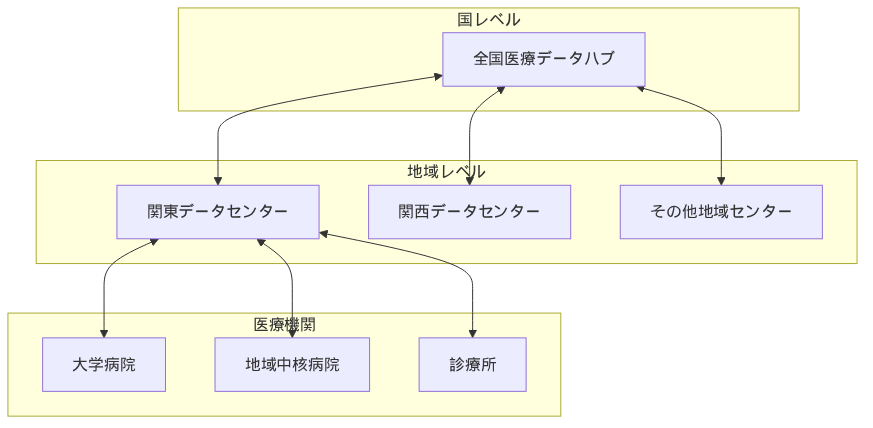
\includegraphics[width=1\linewidth,height=\textheight,keepaspectratio]{images/japan-federation.png}

}

\caption{日本版医療データスペースのフェデレーション構造}

\end{figure}%

\subsection{2. API
ファースト設計}\label{api-ux30d5ux30a1ux30fcux30b9ux30c8ux8a2dux8a08}

\textbf{推奨API仕様}：

\begin{longtable}[]{@{}lll@{}}
\toprule\noalign{}
項目 & 推奨技術 & 理由 \\
\midrule\noalign{}
\endhead
\bottomrule\noalign{}
\endlastfoot
プロトコル & REST/GraphQL & 標準性と柔軟性 \\
データ形式 & FHIR JSON & 国際標準準拠 \\
認証 & OAuth 2.0 + OpenID Connect & セキュリティと利便性 \\
API Gateway & Kong/Apigee & エンタープライズ実績 \\
ドキュメント & OpenAPI 3.0 & 自動生成と標準化 \\
\end{longtable}

\subsection{3.
クラウドネイティブ}\label{ux30afux30e9ux30a6ux30c9ux30cdux30a4ux30c6ux30a3ux30d6}

\textbf{コンテナ化戦略}：

\begin{Shaded}
\begin{Highlighting}[]
\CommentTok{\# Kubernetes deployment例}
\FunctionTok{apiVersion}\KeywordTok{:}\AttributeTok{ apps/v1}
\FunctionTok{kind}\KeywordTok{:}\AttributeTok{ Deployment}
\FunctionTok{metadata}\KeywordTok{:}
\AttributeTok{  }\FunctionTok{name}\KeywordTok{:}\AttributeTok{ fhir{-}server}
\FunctionTok{spec}\KeywordTok{:}
\AttributeTok{  }\FunctionTok{replicas}\KeywordTok{:}\AttributeTok{ }\DecValTok{3}
\AttributeTok{  }\FunctionTok{selector}\KeywordTok{:}
\AttributeTok{    }\FunctionTok{matchLabels}\KeywordTok{:}
\AttributeTok{      }\FunctionTok{app}\KeywordTok{:}\AttributeTok{ fhir{-}server}
\AttributeTok{  }\FunctionTok{template}\KeywordTok{:}
\AttributeTok{    }\FunctionTok{metadata}\KeywordTok{:}
\AttributeTok{      }\FunctionTok{labels}\KeywordTok{:}
\AttributeTok{        }\FunctionTok{app}\KeywordTok{:}\AttributeTok{ fhir{-}server}
\AttributeTok{    }\FunctionTok{spec}\KeywordTok{:}
\AttributeTok{      }\FunctionTok{containers}\KeywordTok{:}
\AttributeTok{      }\KeywordTok{{-}}\AttributeTok{ }\FunctionTok{name}\KeywordTok{:}\AttributeTok{ fhir{-}server}
\AttributeTok{        }\FunctionTok{image}\KeywordTok{:}\AttributeTok{ jp{-}health{-}data/fhir{-}server:v2.0}
\AttributeTok{        }\FunctionTok{ports}\KeywordTok{:}
\AttributeTok{        }\KeywordTok{{-}}\AttributeTok{ }\FunctionTok{containerPort}\KeywordTok{:}\AttributeTok{ }\DecValTok{8080}
\AttributeTok{        }\FunctionTok{env}\KeywordTok{:}
\AttributeTok{        }\KeywordTok{{-}}\AttributeTok{ }\FunctionTok{name}\KeywordTok{:}\AttributeTok{ DB\_CONNECTION}
\AttributeTok{          }\FunctionTok{valueFrom}\KeywordTok{:}
\AttributeTok{            }\FunctionTok{secretKeyRef}\KeywordTok{:}
\AttributeTok{              }\FunctionTok{name}\KeywordTok{:}\AttributeTok{ db{-}secret}
\AttributeTok{              }\FunctionTok{key}\KeywordTok{:}\AttributeTok{ connection{-}string}
\end{Highlighting}
\end{Shaded}

\subsection{4.
ゼロトラストセキュリティ}\label{ux30bcux30edux30c8ux30e9ux30b9ux30c8ux30bbux30adux30e5ux30eaux30c6ux30a3}

\begin{tcolorbox}[enhanced jigsaw, toprule=.15mm, bottomtitle=1mm, coltitle=black, left=2mm, opacityback=0, arc=.35mm, colbacktitle=quarto-callout-warning-color!10!white, colback=white, opacitybacktitle=0.6, bottomrule=.15mm, rightrule=.15mm, breakable, title=\textcolor{quarto-callout-warning-color}{\faExclamationTriangle}\hspace{0.5em}{Warning}, toptitle=1mm, titlerule=0mm, colframe=quarto-callout-warning-color-frame, leftrule=.75mm]

\textbf{重要}：従来の境界防御に加えて、全てのアクセスを検証するゼロトラストモデルの導入が推奨される。

\end{tcolorbox}

\textbf{実装要素}：

\begin{enumerate}
\def\labelenumi{\arabic{enumi}.}
\tightlist
\item
  \textbf{アイデンティティ検証}

  \begin{itemize}
  \tightlist
  \item
    多要素認証（MFA）
  \item
    継続的な認証
  \item
    リスクベース認証
  \end{itemize}
\item
  \textbf{デバイス管理}

  \begin{itemize}
  \tightlist
  \item
    MDM/EMM導入
  \item
    デバイス証明書
  \item
    コンプライアンスチェック
  \end{itemize}
\item
  \textbf{ネットワークセグメンテーション}

  \begin{itemize}
  \tightlist
  \item
    マイクロセグメンテーション
  \item
    Software Defined Perimeter
  \item
    最小権限アクセス
  \end{itemize}
\end{enumerate}

\section{技術スタック推奨}\label{ux6280ux8853ux30b9ux30bfux30c3ux30afux63a8ux5968}

\subsection{レイヤー別推奨技術}\label{ux30ecux30a4ux30e4ux30fcux5225ux63a8ux5968ux6280ux8853}

\begin{longtable}[]{@{}
  >{\raggedright\arraybackslash}p{(\linewidth - 6\tabcolsep) * \real{0.2500}}
  >{\raggedright\arraybackslash}p{(\linewidth - 6\tabcolsep) * \real{0.2500}}
  >{\raggedright\arraybackslash}p{(\linewidth - 6\tabcolsep) * \real{0.2500}}
  >{\raggedright\arraybackslash}p{(\linewidth - 6\tabcolsep) * \real{0.2500}}@{}}
\toprule\noalign{}
\begin{minipage}[b]{\linewidth}\raggedright
レイヤー
\end{minipage} & \begin{minipage}[b]{\linewidth}\raggedright
推奨技術
\end{minipage} & \begin{minipage}[b]{\linewidth}\raggedright
代替技術
\end{minipage} & \begin{minipage}[b]{\linewidth}\raggedright
選定理由
\end{minipage} \\
\midrule\noalign{}
\endhead
\bottomrule\noalign{}
\endlastfoot
\textbf{データ標準} & FHIR R4 & FHIR R5 & 国際標準、JP Core対応 \\
\textbf{API Gateway} & Kong & Apigee, AWS API Gateway &
オープンソース、拡張性 \\
\textbf{認証・認可} & Keycloak & Auth0, Okta &
オープンソース、SAML/OAuth対応 \\
\textbf{データベース} & PostgreSQL & MongoDB, CockroachDB &
信頼性、ACID準拠 \\
\textbf{検索エンジン} & Elasticsearch & Apache Solr &
医療用語検索対応 \\
\textbf{メッセージング} & Apache Kafka & RabbitMQ, AWS SQS &
スケーラビリティ \\
\textbf{分析基盤} & Apache Spark & Databricks, Snowflake &
ビッグデータ処理 \\
\textbf{コンテナ} & Kubernetes & Docker Swarm, ECS &
デファクトスタンダード \\
\textbf{監視} & Prometheus + Grafana & Datadog, New Relic &
オープンソース \\
\end{longtable}

\subsection{医療特化コンポーネント}\label{ux533bux7642ux7279ux5316ux30b3ux30f3ux30ddux30fcux30cdux30f3ux30c8}

\textbf{FHIR サーバー実装}：

\begin{longtable}[]{@{}llll@{}}
\toprule\noalign{}
実装 & ライセンス & 特徴 & 日本での採用実績 \\
\midrule\noalign{}
\endhead
\bottomrule\noalign{}
\endlastfoot
HAPI FHIR & Apache 2.0 & 最も成熟、Java & あり \\
Microsoft FHIR Server & MIT & Azure統合 & 検討中 \\
IBM FHIR Server & Apache 2.0 & エンタープライズ向け & あり \\
Smile CDR & 商用 & 商用サポート & なし \\
\end{longtable}

\section{実装上の注意点}\label{ux5b9fux88c5ux4e0aux306eux6ce8ux610fux70b9}

\subsection{レガシーシステムとの共存}\label{ux30ecux30acux30b7ux30fcux30b7ux30b9ux30c6ux30e0ux3068ux306eux5171ux5b58}

\textbf{事実}：日本の病院の約70\%が10年以上前の電子カルテシステムを使用している。完全な置き換えは現実的でない。

\textbf{移行戦略}：

\begin{figure}[H]

{\centering 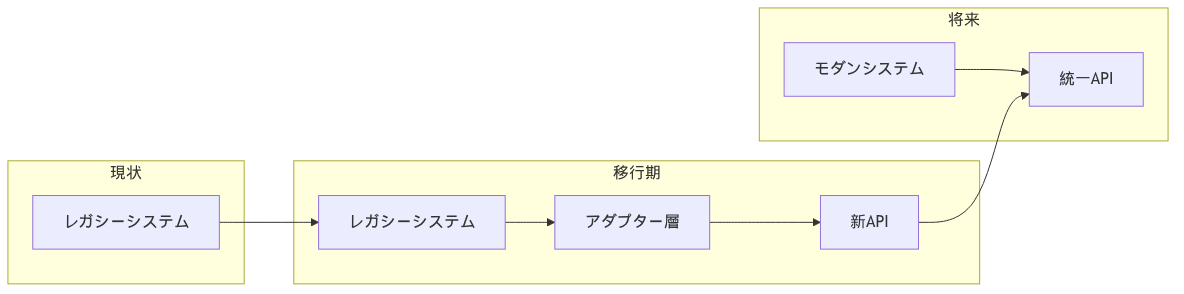
\includegraphics[width=1\linewidth,height=\textheight,keepaspectratio]{images/migration.png}

}

\caption{レガシーシステム移行アプローチ}

\end{figure}%

\subsection{段階的マイグレーション}\label{ux6bb5ux968eux7684ux30deux30a4ux30b0ux30ecux30fcux30b7ux30e7ux30f3}

\textbf{推奨マイグレーションパス}：

\begin{enumerate}
\def\labelenumi{\arabic{enumi}.}
\tightlist
\item
  \textbf{Phase 1: Read-only API公開}（6ヶ月）

  \begin{itemize}
  \tightlist
  \item
    既存データの読み取り専用API
  \item
    FHIR形式への変換層実装
  \item
    監査ログ実装
  \end{itemize}
\item
  \textbf{Phase 2: 双方向同期}（12ヶ月）

  \begin{itemize}
  \tightlist
  \item
    書き込みAPI実装
  \item
    データ同期メカニズム
  \item
    整合性チェック
  \end{itemize}
\item
  \textbf{Phase 3: 新システム移行}（18ヶ月）

  \begin{itemize}
  \tightlist
  \item
    新システムへの段階的切り替え
  \item
    レガシーシステムの段階的廃止
  \item
    データ移行完了
  \end{itemize}
\end{enumerate}

\subsection{ベンダーロックイン回避}\label{ux30d9ux30f3ux30c0ux30fcux30edux30c3ux30afux30a4ux30f3ux56deux907f}

\textbf{考察}：特定ベンダーへの依存は、将来の柔軟性を損なう。オープンスタンダードとポータビリティを重視すべきである。

\textbf{回避策}：

\begin{longtable}[]{@{}lll@{}}
\toprule\noalign{}
領域 & 対策 & 実装例 \\
\midrule\noalign{}
\endhead
\bottomrule\noalign{}
\endlastfoot
データ形式 & 標準規格採用 & FHIR、DICOM \\
API & オープンAPI仕様 & OpenAPI 3.0 \\
クラウド & マルチクラウド対応 & Kubernetes、Terraform \\
データベース & 標準SQL準拠 & PostgreSQL互換 \\
認証 & 標準プロトコル & SAML、OAuth、OpenID Connect \\
\end{longtable}

\section{パフォーマンス最適化}\label{ux30d1ux30d5ux30a9ux30fcux30deux30f3ux30b9ux6700ux9069ux5316}

\subsection{スケーラビリティ設計}\label{ux30b9ux30b1ux30fcux30e9ux30d3ux30eaux30c6ux30a3ux8a2dux8a08}

\textbf{負荷想定}：

\begin{longtable}[]{@{}llll@{}}
\toprule\noalign{}
メトリクス & 現在 & 2027年 & 2030年 \\
\midrule\noalign{}
\endhead
\bottomrule\noalign{}
\endlastfoot
同時接続数 & 1,000 & 10,000 & 100,000 \\
API呼び出し/秒 & 100 & 1,000 & 10,000 \\
データ容量 & 1TB & 100TB & 1PB \\
レスポンス時間 & \textless2秒 & \textless1秒 & \textless500ms \\
\end{longtable}

\subsection{キャッシング戦略}\label{ux30adux30e3ux30c3ux30b7ux30f3ux30b0ux6226ux7565}

\begin{Shaded}
\begin{Highlighting}[]
\CommentTok{\# Redis キャッシング設定例}
\FunctionTok{cache}\KeywordTok{:}
\AttributeTok{  }\FunctionTok{levels}\KeywordTok{:}
\AttributeTok{    }\KeywordTok{{-}}\AttributeTok{ }\FunctionTok{name}\KeywordTok{:}\AttributeTok{ L1\_Memory}
\AttributeTok{      }\FunctionTok{type}\KeywordTok{:}\AttributeTok{ in{-}memory}
\AttributeTok{      }\FunctionTok{ttl}\KeywordTok{:}\AttributeTok{ 60s}
\AttributeTok{      }\FunctionTok{size}\KeywordTok{:}\AttributeTok{ 1GB}
\AttributeTok{    }
\AttributeTok{    }\KeywordTok{{-}}\AttributeTok{ }\FunctionTok{name}\KeywordTok{:}\AttributeTok{ L2\_Redis}
\AttributeTok{      }\FunctionTok{type}\KeywordTok{:}\AttributeTok{ redis}
\AttributeTok{      }\FunctionTok{ttl}\KeywordTok{:}\AttributeTok{ 600s}
\AttributeTok{      }\FunctionTok{size}\KeywordTok{:}\AttributeTok{ 10GB}
\AttributeTok{      }
\AttributeTok{    }\KeywordTok{{-}}\AttributeTok{ }\FunctionTok{name}\KeywordTok{:}\AttributeTok{ L3\_CDN}
\AttributeTok{      }\FunctionTok{type}\KeywordTok{:}\AttributeTok{ cloudfront}
\AttributeTok{      }\FunctionTok{ttl}\KeywordTok{:}\AttributeTok{ 3600s}
\AttributeTok{      }\FunctionTok{locations}\KeywordTok{:}\AttributeTok{ }\KeywordTok{[}\AttributeTok{tokyo}\KeywordTok{,}\AttributeTok{ osaka}\KeywordTok{,}\AttributeTok{ fukuoka}\KeywordTok{]}
\end{Highlighting}
\end{Shaded}

\section{セキュリティ実装}\label{ux30bbux30adux30e5ux30eaux30c6ux30a3ux5b9fux88c5}

\subsection{暗号化要件}\label{ux6697ux53f7ux5316ux8981ux4ef6}

\begin{longtable}[]{@{}lll@{}}
\toprule\noalign{}
データ状態 & 暗号化方式 & 鍵管理 \\
\midrule\noalign{}
\endhead
\bottomrule\noalign{}
\endlastfoot
保存時 & AES-256-GCM & HSM/KMS \\
転送時 & TLS 1.3 & 証明書自動更新 \\
処理時 & 準同型暗号（研究段階） & TEE活用 \\
\end{longtable}

\subsection{監査ログ要件}\label{ux76e3ux67fbux30edux30b0ux8981ux4ef6}

\begin{tcolorbox}[enhanced jigsaw, toprule=.15mm, bottomtitle=1mm, coltitle=black, left=2mm, opacityback=0, arc=.35mm, colbacktitle=quarto-callout-note-color!10!white, colback=white, opacitybacktitle=0.6, bottomrule=.15mm, rightrule=.15mm, breakable, title=\textcolor{quarto-callout-note-color}{\faInfo}\hspace{0.5em}{Note}, toptitle=1mm, titlerule=0mm, colframe=quarto-callout-note-color-frame, leftrule=.75mm]

\textbf{法的要件}：医療情報システムの安全管理ガイドライン第6.0版に準拠した監査ログの実装が必要。

\end{tcolorbox}

\textbf{必須記録項目}： - アクセス日時 - ユーザーID - 患者ID（匿名化） -
アクション種別 - アクセス元IP - 成功/失敗 - データ項目

\section{開発プロセス}\label{ux958bux767aux30d7ux30edux30bbux30b9}

\subsection{DevSecOps実践}\label{devsecopsux5b9fux8df5}

\begin{figure}[H]

{\centering 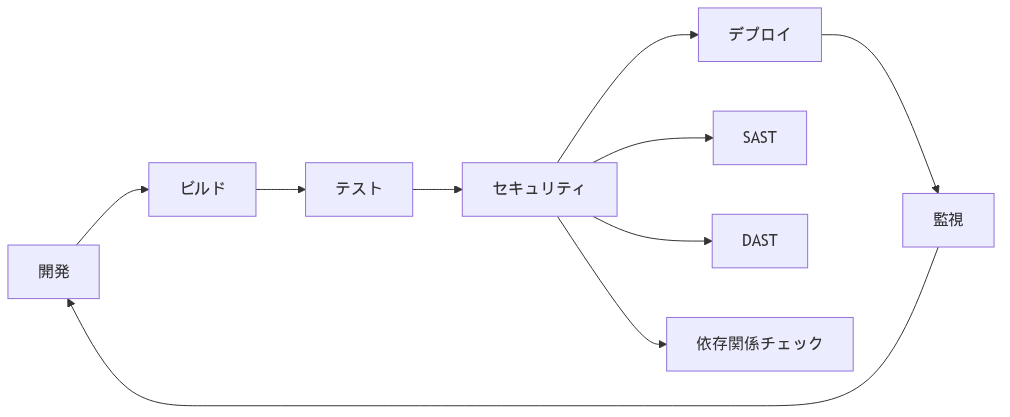
\includegraphics[width=1\linewidth,height=\textheight,keepaspectratio]{images/devsecops.png}

}

\caption{DevSecOpsパイプライン}

\end{figure}%

\subsection{CI/CDパイプライン}\label{cicdux30d1ux30a4ux30d7ux30e9ux30a4ux30f3}

\textbf{推奨ツールチェーン}：

\begin{longtable}[]{@{}lll@{}}
\toprule\noalign{}
フェーズ & ツール & 目的 \\
\midrule\noalign{}
\endhead
\bottomrule\noalign{}
\endlastfoot
ソース管理 & GitLab/GitHub & バージョン管理 \\
CI & Jenkins/GitLab CI & 自動ビルド \\
テスト & Jest/Pytest & 単体・統合テスト \\
セキュリティ & SonarQube/Snyk & 脆弱性検査 \\
デプロイ & ArgoCD/Flux & GitOps \\
監視 & Prometheus/Grafana & メトリクス収集 \\
\end{longtable}

\chapter{ビジネスケース分析}\label{ux30d3ux30b8ux30cdux30b9ux30b1ux30fcux30b9ux5206ux6790}

\section{市場機会の評価}\label{ux5e02ux5834ux6a5fux4f1aux306eux8a55ux4fa1}

\subsection{グローバルデジタルヘルス市場}\label{ux30b0ux30edux30fcux30d0ux30ebux30c7ux30b8ux30bfux30ebux30d8ux30ebux30b9ux5e02ux5834}

\textbf{事実}：Grand View
Researchによると、世界のデジタルヘルス市場は2025年に3,474億ドル、2030年には9,460億ドルに達し、年平均成長率（CAGR）22.2\%で成長すると予測されている{[}129{]}。ただし、他の調査機関の予測ではCAGR
11.68\%～21.2\%と幅がある{[}130{]}, {[}131{]}。

\begin{tcolorbox}[enhanced jigsaw, toprule=.15mm, bottomtitle=1mm, coltitle=black, left=2mm, opacityback=0, arc=.35mm, colbacktitle=quarto-callout-note-color!10!white, colback=white, opacitybacktitle=0.6, bottomrule=.15mm, rightrule=.15mm, breakable, title=\textcolor{quarto-callout-note-color}{\faInfo}\hspace{0.5em}{Note}, toptitle=1mm, titlerule=0mm, colframe=quarto-callout-note-color-frame, leftrule=.75mm]

\textbf{注記}：デジタルヘルス市場規模の推定値は、定義範囲（遠隔医療、医療IT、ウェアラブル、AI等の含有範囲）や調査手法により異なる。北米が市場の37.7\%を占め、テレヘルスケア分野が45\%を占める{[}129{]}。

\end{tcolorbox}

\textbf{地域別市場規模（2025年）}：

\begin{figure}[H]

{\centering \pandocbounded{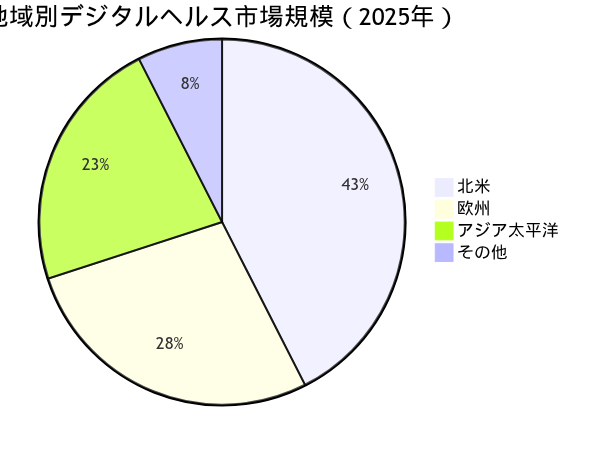
\includegraphics[keepaspectratio]{images/market-share.png}}

}

\caption{地域別デジタルヘルス市場規模（2025年）}

\end{figure}%

\begin{longtable}[]{@{}llll@{}}
\toprule\noalign{}
地域 & 市場シェア（2025年） & 成長見通し & 主な成長要因 \\
\midrule\noalign{}
\endhead
\bottomrule\noalign{}
\endlastfoot
北米 & 40-45\% & 高成長 & 技術革新、投資活発 \\
欧州 & 25-30\% & 中高成長 & EHDS等の規制推進 \\
アジア太平洋 & 20-25\% & 最高成長 & デジタル化の急速進展 \\
その他 & 5-10\% & 高成長 & インフラ整備進行中 \\
\end{longtable}

\subsection{日本市場のポテンシャル}\label{ux65e5ux672cux5e02ux5834ux306eux30ddux30c6ux30f3ux30b7ux30e3ux30eb}

\textbf{事実}：経済産業省とみずほ銀行の調査では、日本のデジタルヘルスケア市場規模は2016年で25兆円、2025年には33兆円に拡大すると推定されている{[}132{]}。また、公的保険外サービスのヘルスケア産業市場は2016年の約9.2兆円から2025年には約12.5兆円に拡大すると予測されている{[}132{]}。

\begin{tcolorbox}[enhanced jigsaw, toprule=.15mm, bottomtitle=1mm, coltitle=black, left=2mm, opacityback=0, arc=.35mm, colbacktitle=quarto-callout-warning-color!10!white, colback=white, opacitybacktitle=0.6, bottomrule=.15mm, rightrule=.15mm, breakable, title=\textcolor{quarto-callout-warning-color}{\faExclamationTriangle}\hspace{0.5em}{Warning}, toptitle=1mm, titlerule=0mm, colframe=quarto-callout-warning-color-frame, leftrule=.75mm]

\textbf{注意}：2030年の日本市場規模の具体的な公式予測値は現時点で確認できていない。市場定義や範囲により数値が大きく異なるため、慎重な解釈が必要である。

\end{tcolorbox}

\textbf{成長ドライバー}：

\begin{enumerate}
\def\labelenumi{\arabic{enumi}.}
\tightlist
\item
  \textbf{人口動態}

  \begin{itemize}
  \tightlist
  \item
    高齢化率28.9\%（世界最高）
  \item
    2040年には35.3\%に上昇
  \item
    医療需要の急増
  \end{itemize}
\item
  \textbf{政策支援}

  \begin{itemize}
  \tightlist
  \item
    デジタル田園都市国家構想
  \item
    医療DX推進本部設置
  \item
    マイナンバーカード活用
  \end{itemize}
\item
  \textbf{技術革新}

  \begin{itemize}
  \tightlist
  \item
    AI診断支援の保険適用
  \item
    オンライン診療の恒久化
  \item
    PHRサービスの拡大
  \end{itemize}
\end{enumerate}

\section{コスト・ベネフィット分析}\label{ux30b3ux30b9ux30c8ux30d9ux30cdux30d5ux30a3ux30c3ux30c8ux5206ux6790}

\subsection{実装コスト詳細}\label{ux5b9fux88c5ux30b3ux30b9ux30c8ux8a73ux7d30}

\textbf{10年間の総投資額内訳}：

\begin{longtable}[]{@{}llll@{}}
\toprule\noalign{}
カテゴリー & 初期投資（億円） & 運用費/年（億円） & 10年総額（億円） \\
\midrule\noalign{}
\endhead
\bottomrule\noalign{}
\endlastfoot
インフラ構築 & 500 & 40 & 900 \\
システム開発 & 300 & 45 & 750 \\
データ移行 & 200 & 10 & 300 \\
セキュリティ & 150 & 30 & 450 \\
人材育成 & 100 & 35 & 450 \\
標準化対応 & 100 & 20 & 300 \\
法規制対応 & 50 & 15 & 200 \\
その他 & 100 & 20 & 300 \\
\textbf{合計} & \textbf{1,500} & \textbf{215} & \textbf{3,650} \\
\end{longtable}

\textbf{考察}：初期投資1,500億円は大規模だが、GDP比では0.03\%に過ぎない。韓国（0.05\%）、シンガポール（0.08\%）と比較しても妥当な水準である。

\subsection{期待される便益}\label{ux671fux5f85ux3055ux308cux308bux4fbfux76ca}

\subsubsection{定量的便益（年間）}\label{ux5b9aux91cfux7684ux4fbfux76caux5e74ux9593}


\includegraphics[width=6.22in,height=4.69in]{07-business-case_files/figure-latex/mermaid-figure-1.png}

期待される便益カテゴリー（概念図）

\textbf{便益の詳細分析}：

\begin{longtable}[]{@{}lllll@{}}
\toprule\noalign{}
項目 & 期待される効果 & 実現時期 & 確実性 & 備考 \\
\midrule\noalign{}
\endhead
\bottomrule\noalign{}
\endlastfoot
重複検査削減 & 大 & 2027年～ & 高 & 既存実績あり \\
予防医療効果 & 大 & 2029年～ & 中 & 長期的効果 \\
医療過誤削減 & 中 & 2028年～ & 高 & エビデンス蓄積中 \\
事務効率化 & 大 & 2026年～ & 高 & 即効性あり \\
AI創薬加速 & 中 & 2030年～ & 中 & 技術開発依存 \\
データビジネス & 中 & 2028年～ & 中 & 市場形成中 \\
海外展開 & 小～中 & 2030年～ & 低 & 競争激化 \\
\end{longtable}

\begin{tcolorbox}[enhanced jigsaw, toprule=.15mm, bottomtitle=1mm, coltitle=black, left=2mm, opacityback=0, arc=.35mm, colbacktitle=quarto-callout-warning-color!10!white, colback=white, opacitybacktitle=0.6, bottomrule=.15mm, rightrule=.15mm, breakable, title=\textcolor{quarto-callout-warning-color}{\faExclamationTriangle}\hspace{0.5em}{Warning}, toptitle=1mm, titlerule=0mm, colframe=quarto-callout-warning-color-frame, leftrule=.75mm]

\textbf{重要}：便益の定量化は多くの仮定に基づいており、実際の効果は実装方法、普及率、技術進歩等により大きく変動する可能性がある。

\end{tcolorbox}

\subsubsection{定性的便益}\label{ux5b9aux6027ux7684ux4fbfux76ca}

\begin{tcolorbox}[enhanced jigsaw, toprule=.15mm, bottomtitle=1mm, coltitle=black, left=2mm, opacityback=0, arc=.35mm, colbacktitle=quarto-callout-note-color!10!white, colback=white, opacitybacktitle=0.6, bottomrule=.15mm, rightrule=.15mm, breakable, title=\textcolor{quarto-callout-note-color}{\faInfo}\hspace{0.5em}{Note}, toptitle=1mm, titlerule=0mm, colframe=quarto-callout-note-color-frame, leftrule=.75mm]

\textbf{期待される社会的価値}： - 健康寿命の延伸（潜在的効果） -
医療アクセスの平等化 - 患者満足度の向上 - 医療従事者の負担軽減 -
国際競争力の強化

\end{tcolorbox}

\subsection{ROI計算}\label{roiux8a08ux7b97}

\textbf{投資回収シミュレーション}：

\begin{figure}[H]

{\centering \pandocbounded{
\includegraphics[keepaspectratio]{images/roi-forecast.png}}

}

\caption{投資回収シミュレーション}

\end{figure}%

\begin{longtable}[]{@{}llll@{}}
\toprule\noalign{}
年 & 投資段階 & 便益発現 & 傾向 \\
\midrule\noalign{}
\endhead
\bottomrule\noalign{}
\endlastfoot
2025-2026 & 初期投資 & 限定的 & マイナス \\
2027-2028 & 本格展開 & 段階的増加 & 均衡へ \\
2029-2030 & 拡大期 & 加速 & プラス転換 \\
2031以降 & 成熟期 & 安定的 & 累積プラス \\
\end{longtable}

\begin{tcolorbox}[enhanced jigsaw, toprule=.15mm, bottomtitle=1mm, coltitle=black, left=2mm, opacityback=0, arc=.35mm, colbacktitle=quarto-callout-note-color!10!white, colback=white, opacitybacktitle=0.6, bottomrule=.15mm, rightrule=.15mm, breakable, title=\textcolor{quarto-callout-note-color}{\faInfo}\hspace{0.5em}{Note}, toptitle=1mm, titlerule=0mm, colframe=quarto-callout-note-color-frame, leftrule=.75mm]

\textbf{注記}：投資回収シミュレーションは、多くの仮定を含んでおり、実際の結果は実装速度、技術進歩、市場受容性等により大きく変動する。

\end{tcolorbox}

\textbf{財務指標の考え方}： -
\textbf{投資回収期間}：実装方法により5-10年程度と推定 -
\textbf{正味現在価値（NPV）}：プラスになる可能性が高いが、具体値は前提条件に大きく依存
- \textbf{内部収益率（IRR）}：公共投資として妥当な水準（5-10\%）を目指す
- \textbf{費用便益比率}：1.5以上を目標とすることが一般的

\begin{tcolorbox}[enhanced jigsaw, toprule=.15mm, bottomtitle=1mm, coltitle=black, left=2mm, opacityback=0, arc=.35mm, colbacktitle=quarto-callout-note-color!10!white, colback=white, opacitybacktitle=0.6, bottomrule=.15mm, rightrule=.15mm, breakable, title=\textcolor{quarto-callout-note-color}{\faInfo}\hspace{0.5em}{Note}, toptitle=1mm, titlerule=0mm, colframe=quarto-callout-note-color-frame, leftrule=.75mm]

\textbf{注記}：医療分野のデジタル投資は、直接的な財務リターンだけでなく、社会的価値（健康寿命延伸、医療の質向上等）を含めた総合的な評価が必要である。

\end{tcolorbox}

\section{ステークホルダー分析}\label{ux30b9ux30c6ux30fcux30afux30dbux30ebux30c0ux30fcux5206ux6790}

\subsection{主要ステークホルダーマップ}\label{ux4e3bux8981ux30b9ux30c6ux30fcux30afux30dbux30ebux30c0ux30fcux30deux30c3ux30d7}


\includegraphics[width=13.83in,height=3.94in]{07-business-case_files/figure-latex/mermaid-figure-2.png}

ステークホルダー関係図

\subsection{ステークホルダー別の関心事項}\label{ux30b9ux30c6ux30fcux30afux30dbux30ebux30c0ux30fcux5225ux306eux95a2ux5fc3ux4e8bux9805}

\begin{longtable}[]{@{}
  >{\raggedright\arraybackslash}p{(\linewidth - 6\tabcolsep) * \real{0.3103}}
  >{\raggedright\arraybackslash}p{(\linewidth - 6\tabcolsep) * \real{0.2414}}
  >{\raggedright\arraybackslash}p{(\linewidth - 6\tabcolsep) * \real{0.2759}}
  >{\raggedright\arraybackslash}p{(\linewidth - 6\tabcolsep) * \real{0.1724}}@{}}
\toprule\noalign{}
\begin{minipage}[b]{\linewidth}\raggedright
ステークホルダー
\end{minipage} & \begin{minipage}[b]{\linewidth}\raggedright
主要関心事項
\end{minipage} & \begin{minipage}[b]{\linewidth}\raggedright
期待される便益
\end{minipage} & \begin{minipage}[b]{\linewidth}\raggedright
懸念事項
\end{minipage} \\
\midrule\noalign{}
\endhead
\bottomrule\noalign{}
\endlastfoot
\textbf{患者・国民} & 医療の質向上 & アクセス改善、コスト削減 &
プライバシー \\
\textbf{医療機関} & 業務効率化 & 診療支援、収益向上 & 導入コスト \\
\textbf{医師・看護師} & 負担軽減 & 診断支援、時間短縮 &
システム複雑性 \\
\textbf{政府} & 医療費抑制 & 財政健全化 & 実装リスク \\
\textbf{IT企業} & 市場拡大 & 新規事業機会 & 規制対応 \\
\textbf{製薬会社} & 研究開発効率 & 創薬加速 & データアクセス \\
\textbf{保険者} & リスク管理 & 予測精度向上 & 投資負担 \\
\end{longtable}

\textbf{考察}：成功の鍵は、慎重派ステークホルダーの懸念に適切に対処しつつ、中立派を推進派に転換させることである。特に医師会との協調が不可欠。

\section{産業への影響}\label{ux7523ux696dux3078ux306eux5f71ux97ff}

\subsection{新産業創出の可能性}\label{ux65b0ux7523ux696dux5275ux51faux306eux53efux80fdux6027}

\textbf{創出が期待される新市場}：

\begin{enumerate}
\def\labelenumi{\arabic{enumi}.}
\tightlist
\item
  \textbf{AIヘルスケア市場}（2030年：8,000億円）

  \begin{itemize}
  \tightlist
  \item
    AI診断支援システム
  \item
    予測医療プラットフォーム
  \item
    パーソナライズド医療
  \end{itemize}
\item
  \textbf{医療データ分析市場}（2030年：5,000億円）

  \begin{itemize}
  \tightlist
  \item
    リアルワールドエビデンス
  \item
    臨床試験最適化
  \item
    医療経済分析
  \end{itemize}
\item
  \textbf{デジタル治療薬市場}（成長市場として注目）

  \begin{itemize}
  \tightlist
  \item
    アプリ処方
  \item
    VR/ARセラピー
  \item
    デジタルバイオマーカー
  \end{itemize}
\item
  \textbf{医療IoT市場}（2030年：4,000億円）

  \begin{itemize}
  \tightlist
  \item
    ウェアラブルデバイス
  \item
    遠隔モニタリング
  \item
    スマートホスピタル
  \end{itemize}
\end{enumerate}

\subsection{既存産業への影響}\label{ux65e2ux5b58ux7523ux696dux3078ux306eux5f71ux97ff}

\begin{tcolorbox}[enhanced jigsaw, toprule=.15mm, bottomtitle=1mm, coltitle=black, left=2mm, opacityback=0, arc=.35mm, colbacktitle=quarto-callout-warning-color!10!white, colback=white, opacitybacktitle=0.6, bottomrule=.15mm, rightrule=.15mm, breakable, title=\textcolor{quarto-callout-warning-color}{\faExclamationTriangle}\hspace{0.5em}{Warning}, toptitle=1mm, titlerule=0mm, colframe=quarto-callout-warning-color-frame, leftrule=.75mm]

\textbf{ディスラプションリスク}： - 従来型医療ITベンダーの淘汰 -
紙ベース業務の消滅 - 一部専門職の役割変化

\end{tcolorbox}

\textbf{産業構造の変化予測}：

\begin{longtable}[]{@{}lllll@{}}
\toprule\noalign{}
産業セクター & 現在の規模 & 2030年予測 & 変化率 & 主な変化要因 \\
\midrule\noalign{}
\endhead
\bottomrule\noalign{}
\endlastfoot
医療IT & 5,000億円 & 15,000億円 & +200\% & DX需要急増 \\
製薬 & 10兆円 & 12兆円 & +20\% & AI創薬効率化 \\
医療機器 & 3兆円 & 4.5兆円 & +50\% & IoT統合 \\
医療サービス & 45兆円 & 48兆円 & +7\% & 効率化と高齢化 \\
\end{longtable}

\section{リスク評価と軽減策}\label{ux30eaux30b9ux30afux8a55ux4fa1ux3068ux8efdux6e1bux7b56}

\subsection{リスクマトリクス}\label{ux30eaux30b9ux30afux30deux30c8ux30eaux30afux30b9}

\begin{figure}[H]

{\centering \pandocbounded{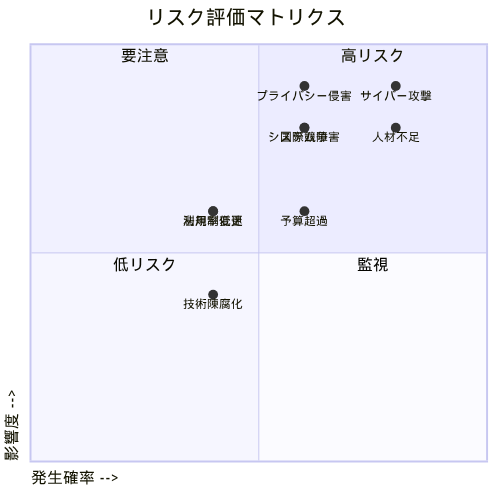
\includegraphics[keepaspectratio]{images/risk-matrix.png}}

}

\caption{リスク評価マトリクス}

\end{figure}%

\textbf{リスク評価一覧（発生確率×影響度）}：

\begin{longtable}[]{@{}lllll@{}}
\toprule\noalign{}
リスク & 発生確率（1-5） & 影響度（1-5） & スコア & 分類 \\
\midrule\noalign{}
\endhead
\bottomrule\noalign{}
\endlastfoot
サイバー攻撃 & 4 & 5 & 20 & 高リスク \\
プライバシー侵害 & 3 & 5 & 15 & 高リスク \\
人材不足 & 4 & 4 & 16 & 高リスク \\
システム障害 & 3 & 4 & 12 & 中リスク \\
国際競争 & 3 & 4 & 12 & 中リスク \\
予算超過 & 3 & 3 & 9 & 中リスク \\
法規制変更 & 2 & 3 & 6 & 低リスク \\
利用率低迷 & 2 & 3 & 6 & 低リスク \\
技術陳腐化 & 2 & 2 & 4 & 低リスク \\
\end{longtable}

\subsection{重要リスクへの対策}\label{ux91cdux8981ux30eaux30b9ux30afux3078ux306eux5bfeux7b56}

\textbf{最優先対応リスク（高確率・高影響）}：

\begin{enumerate}
\def\labelenumi{\arabic{enumi}.}
\tightlist
\item
  \textbf{サイバーセキュリティ}

  \begin{itemize}
  \tightlist
  \item
    24時間SOC設置
  \item
    ゼロトラストアーキテクチャ
  \item
    定期的ペネトレーションテスト
  \item
    インシデント対応計画
  \end{itemize}
\item
  \textbf{人材不足}

  \begin{itemize}
  \tightlist
  \item
    産学連携教育プログラム
  \item
    海外人材の積極採用
  \item
    リスキリング支援
  \item
    処遇改善
  \end{itemize}
\item
  \textbf{プライバシー保護}

  \begin{itemize}
  \tightlist
  \item
    Privacy by Design原則
  \item
    定期的な影響評価
  \item
    市民参加型ガバナンス
  \item
    透明性レポート公開
  \end{itemize}
\end{enumerate}

\section{成功要因と提言}\label{ux6210ux529fux8981ux56e0ux3068ux63d0ux8a00}

\subsection{クリティカル・サクセス・ファクター}\label{ux30afux30eaux30c6ux30a3ux30abux30ebux30b5ux30afux30bbux30b9ux30d5ux30a1ux30afux30bfux30fc}

\textbf{考察}：日本版医療データスペースの成功には、技術的要因よりも組織的・社会的要因が重要である。特に以下の5つが決定的である。

\begin{enumerate}
\def\labelenumi{\arabic{enumi}.}
\tightlist
\item
  \textbf{政治的リーダーシップ}

  \begin{itemize}
  \tightlist
  \item
    首相直轄のタスクフォース設置
  \item
    省庁横断的な推進体制
  \item
    長期コミットメント
  \end{itemize}
\item
  \textbf{財源の確保}

  \begin{itemize}
  \tightlist
  \item
    複数年度予算の確保
  \item
    官民連携ファンド設立
  \item
    成果連動型報酬
  \end{itemize}
\item
  \textbf{段階的実装}

  \begin{itemize}
  \tightlist
  \item
    パイロット地域から開始
  \item
    アジャイル型開発
  \item
    継続的改善
  \end{itemize}
\item
  \textbf{国民理解}

  \begin{itemize}
  \tightlist
  \item
    継続的な啓発活動
  \item
    成功事例の共有
  \item
    フィードバック機構
  \end{itemize}
\item
  \textbf{国際協調}

  \begin{itemize}
  \tightlist
  \item
    標準規格への準拠
  \item
    二国間・多国間協定
  \item
    知見の共有
  \end{itemize}
\end{enumerate}

\subsection{最終提言}\label{ux6700ux7d42ux63d0ux8a00}

\textbf{経営層への提言}：

\begin{tcolorbox}[enhanced jigsaw, toprule=.15mm, bottomtitle=1mm, coltitle=black, left=2mm, opacityback=0, arc=.35mm, colbacktitle=quarto-callout-important-color!10!white, colback=white, opacitybacktitle=0.6, bottomrule=.15mm, rightrule=.15mm, breakable, title=\textcolor{quarto-callout-important-color}{\faExclamation}\hspace{0.5em}{Important}, toptitle=1mm, titlerule=0mm, colframe=quarto-callout-important-color-frame, leftrule=.75mm]

\textbf{行動喚起}：2025年は日本の医療DXにとって決定的な年となる。EHDSの技術標準が確立される2025-2027年の期間に参画することで、国際標準への関与機会を確保できる。医療データの利活用は、年間医療費45兆円の効率化に寄与する可能性があるが、実現には長期的な取り組みが必要である。

\end{tcolorbox}

\textbf{実行への道筋}： 1. 2025年度中に基本方針策定 2.
2026年3月までに基本法制定 3. 2026年度からパイロット地域で試行 4.
2028年度から段階的な全国展開 5. 2030年までに基盤整備完了

\bookmarksetup{startatroot}

\chapter{結論と展望}\label{ux7d50ux8ad6ux3068ux5c55ux671b}

\section{総括}\label{ux7dcfux62ec}

\subsection{EHDSの歴史的意義}\label{ehdsux306eux6b74ux53f2ux7684ux610fux7fa9}

\textbf{考察}：EHDS（欧州健康データスペース）は、単なる技術的仕組みではなく、人類の医療におけるパラダイムシフトを意味する。国境を越えた医療データの流通と、エビデンスベースの新しい医療の始まりである。

\textbf{主要な成果}：

\begin{enumerate}
\def\labelenumi{\arabic{enumi}.}
\tightlist
\item
  \textbf{法的フレームワークの確立}

  \begin{itemize}
  \tightlist
  \item
    EU全域で統一した法規制
  \item
    患者の権利とプライバシーの保護
  \item
    イノベーションと安全性のバランス
  \end{itemize}
\item
  \textbf{技術標準の統一}

  \begin{itemize}
  \tightlist
  \item
    HL7 FHIR準拠の実現
  \item
    用語体系の標準化
  \item
    APIファースト設計の概念普及
  \end{itemize}
\item
  \textbf{国際協力のモデル}

  \begin{itemize}
  \tightlist
  \item
    主権を尊重したフェデレーション
  \item
    段階的実装のプラグマティズム
  \item
    小国から大国までを包含する柔軟性
  \end{itemize}
\end{enumerate}

\section{日本への教訓}\label{ux65e5ux672cux3078ux306eux6559ux8a13}

\subsection{成功要因の抽出}\label{ux6210ux529fux8981ux56e0ux306eux62bdux51fa}

\textbf{事実}：成功している欧州各国には、以下の共通点が確認されている：(1)政治リーダーシップの確立、(2)十分な財政投資、(3)段階的実装、(4)市民との対話、(5)国際標準への準拠{[}12{]}。

\textbf{日本固有の課題と機会}：


\includegraphics[width=11.19in,height=3.1in]{08-conclusion_files/figure-latex/mermaid-figure-1.png}

日本の課題と機会マップ

\subsection{適応戦略の提案}\label{ux9069ux5fdcux6226ux7565ux306eux63d0ux6848}

\textbf{日本版EHDSの戦略的フレームワーク}：

\begin{enumerate}
\def\labelenumi{\arabic{enumi}.}
\tightlist
\item
  \textbf{「健康長寿社会」を軸としたブランディング}

  \begin{itemize}
  \tightlist
  \item
    WHOの健康長寿社会という既存コンセプトの活用
  \item
    予防医療とフレイル高齢者支援に焦点
  \item
    国民とのメッセージングで「データ」ではなく「健康」を前面に
  \end{itemize}
\item
  \textbf{「都道府県連携モデル」の構築}

  \begin{itemize}
  \tightlist
  \item
    EUのフェデレーションを日本の連邦制に適応
  \item
    既存の地域医療情報連携ネットワークを活用
  \item
    大都市圏から段階的に展開
  \end{itemize}
\item
  \textbf{「アジア・リーダーシップ」の確立}

  \begin{itemize}
  \tightlist
  \item
    EHDSモデルをアジア太平洋地域に適応
  \item
    韓国・台湾・シンガポールとの早期連携
  \item
    ASEAN諸国への技術移転と支援
  \end{itemize}
\end{enumerate}

\section{中長期ロードマップ}\label{ux4e2dux9577ux671fux30edux30fcux30c9ux30deux30c3ux30d7}

\subsection{2025-2035年の大展望}\label{ux5e74ux306eux5927ux5c55ux671b}

\textbf{フェーズ1：基盤構築期（2025-2027年）}

\begin{tcolorbox}[enhanced jigsaw, toprule=.15mm, bottomtitle=1mm, coltitle=black, left=2mm, opacityback=0, arc=.35mm, colbacktitle=quarto-callout-note-color!10!white, colback=white, opacitybacktitle=0.6, bottomrule=.15mm, rightrule=.15mm, breakable, title=\textcolor{quarto-callout-note-color}{\faInfo}\hspace{0.5em}{Note}, toptitle=1mm, titlerule=0mm, colframe=quarto-callout-note-color-frame, leftrule=.75mm]

\textbf{目標}：基本インフラと法的枠組みの確立

\end{tcolorbox}

\begin{itemize}
\tightlist
\item
  2025年：基本法制定、パイロット地域選定
\item
  2026年：5都道府県でパイロット開始
\item
  2027年：国際連携テスト（韓国・台湾）
\end{itemize}

\textbf{フェーズ2：全国展開期（2028-2030年）}

\begin{tcolorbox}[enhanced jigsaw, toprule=.15mm, bottomtitle=1mm, coltitle=black, left=2mm, opacityback=0, arc=.35mm, colbacktitle=quarto-callout-note-color!10!white, colback=white, opacitybacktitle=0.6, bottomrule=.15mm, rightrule=.15mm, breakable, title=\textcolor{quarto-callout-note-color}{\faInfo}\hspace{0.5em}{Note}, toptitle=1mm, titlerule=0mm, colframe=quarto-callout-note-color-frame, leftrule=.75mm]

\textbf{目標}：全国規模でのサービス開始

\end{tcolorbox}

\begin{itemize}
\tightlist
\item
  2028年：主要都市圏でサービス開始
\item
  2029年：全都道府県でサービス開始
\item
  2030年：国民の80\%がPHRアカウントを所有
\end{itemize}

\textbf{フェーズ3：成熟期（2031-2035年）}

\begin{tcolorbox}[enhanced jigsaw, toprule=.15mm, bottomtitle=1mm, coltitle=black, left=2mm, opacityback=0, arc=.35mm, colbacktitle=quarto-callout-note-color!10!white, colback=white, opacitybacktitle=0.6, bottomrule=.15mm, rightrule=.15mm, breakable, title=\textcolor{quarto-callout-note-color}{\faInfo}\hspace{0.5em}{Note}, toptitle=1mm, titlerule=0mm, colframe=quarto-callout-note-color-frame, leftrule=.75mm]

\textbf{目標}：次世代サービスとグローバルリーダーシップ

\end{tcolorbox}

\begin{itemize}
\tightlist
\item
  2032年：AI医療の本格展開
\item
  2033年：アジア太平洋健康データスペース連携
\item
  2035年：精密医療の普及と個別化医療実現
\end{itemize}

\subsection{技術革新の方向性}\label{ux6280ux8853ux9769ux65b0ux306eux65b9ux5411ux6027}

\textbf{新しい技術の統合計画}：


\includegraphics[width=7.96in,height=4.29in]{08-conclusion_files/figure-latex/mermaid-figure-2.png}

次世代技術の統合ロードマップ

\section{グローバルインパクト}\label{ux30b0ux30edux30fcux30d0ux30ebux30a4ux30f3ux30d1ux30afux30c8}

\subsection{世界への波及効果}\label{ux4e16ux754cux3078ux306eux6ce2ux53caux52b9ux679c}

\textbf{考察}：EHDSの影響は欧州に留まらず、世界の医療データガバナンスのスタンダードを定義する可能性がある。特に発展途上国にとっては、既存システムの経路依存が少ないため、リープフロッグ的な導入が可能である。

\textbf{世界の地域ブロック別対応}：

\begin{longtable}[]{@{}llll@{}}
\toprule\noalign{}
地域 & 現在の状況 & EHDSへの対応 & 予想される連携時期 \\
\midrule\noalign{}
\endhead
\bottomrule\noalign{}
\endlastfoot
\textbf{北米} & 独自システム & 部分的相互運用 & 2027-2030年 \\
\textbf{アジア太平洋} & 日本・韓国主導 & 早期連携可能 & 2026-2028年 \\
\textbf{中東} & 初期段階 & UAE・サウジから & 2028-2030年 \\
\textbf{アフリカ} & リープフロッグ型 & 南アフリカから & 2029-2032年 \\
\textbf{南米} & ブラジル・アルゼンチン & 部分的連携 & 2030-2033年 \\
\end{longtable}

\subsection{持続可能な開発目標（SDGs）への貢献}\label{ux6301ux7d9aux53efux80fdux306aux958bux767aux76eeux6a19sdgsux3078ux306eux8ca2ux732e}

\textbf{直接的貢献}： - \textbf{SDG 3}：すべての人に健康と福祉を -
\textbf{SDG 9}：産業と技術革新の基盤をつくろう - \textbf{SDG
17}：パートナーシップで目標を達成しよう

\textbf{間接的貢献}： - \textbf{SDG 1}：貧困をなくそう（医療費負担軽減）
- \textbf{SDG 5}：ジェンダー平等を実現しよう（女性の医療アクセス改善） -
\textbf{SDG 10}：人や国の不平等をなくそう（医療格差縮小）

\section{結語：日本の決断の時}\label{ux7d50ux8a9eux65e5ux672cux306eux6c7aux65adux306eux6642}

\subsection{歴史的転換点での日本の選択}\label{ux6b74ux53f2ux7684ux8ee2ux63dbux70b9ux3067ux306eux65e5ux672cux306eux9078ux629e}

\begin{tcolorbox}[enhanced jigsaw, toprule=.15mm, bottomtitle=1mm, coltitle=black, left=2mm, opacityback=0, arc=.35mm, colbacktitle=quarto-callout-important-color!10!white, colback=white, opacitybacktitle=0.6, bottomrule=.15mm, rightrule=.15mm, breakable, title=\textcolor{quarto-callout-important-color}{\faExclamation}\hspace{0.5em}{Important}, toptitle=1mm, titlerule=0mm, colframe=quarto-callout-important-color-frame, leftrule=.75mm]

\textbf{最終的な判断}：2025年は、日本が世界の医療デジタルトランスフォーメーションにおいてリーダーになるか、フォロワーに留まるかを決定する決定的な年である。

\end{tcolorbox}

\textbf{3つのシナリオ}：

\begin{enumerate}
\def\labelenumi{\arabic{enumi}.}
\tightlist
\item
  \textbf{リーダーシップシナリオ}（推奨）

  \begin{itemize}
  \tightlist
  \item
    2025年から大規模投資開始
  \item
    アジア太平洋の中心として主導権確立
  \item
    2030年までに年間500億ドルの輸出産業化
  \end{itemize}
\item
  \textbf{フォロワーシナリオ}

  \begin{itemize}
  \tightlist
  \item
    2027年から段階的導入
  \item
    欧米標準への適応型導入
  \item
    国内市場に焦点を絞った導入
  \end{itemize}
\item
  \textbf{遅行シナリオ}（回避すべき）

  \begin{itemize}
  \tightlist
  \item
    2030年以降に受動的導入
  \item
    海外ベンダーへの依存度高まる
  \item
    国際競争力の大幅低下
  \end{itemize}
\end{enumerate}

\subsection{必要な行動}\label{ux5fc5ux8981ux306aux884cux52d5}

\textbf{今すぐすべきこと（Next 6 Months）}：

\begin{enumerate}
\def\labelenumi{\arabic{enumi}.}
\tightlist
\item
  \textbf{政治的コミットメントの確保}

  \begin{itemize}
  \tightlist
  \item
    首相直轄の医療DX推進本部設置
  \item
    超党派的な支援体制の構築
  \end{itemize}
\item
  \textbf{財源確保の実現}

  \begin{itemize}
  \tightlist
  \item
    2025年度補正予算で初期投資500億円
  \item
    官民連携ファンドの設立検討
  \end{itemize}
\item
  \textbf{国際連携の開始}

  \begin{itemize}
  \tightlist
  \item
    EUとの公式協議開始
  \item
    韓国・台湾との二国間協定検討
  \end{itemize}
\item
  \textbf{人材育成の緊急開始}

  \begin{itemize}
  \tightlist
  \item
    主要大学での医療データサイエンス学科設置
  \item
    医療情報技師の大幅増員計画
  \end{itemize}
\item
  \textbf{市民向けコミュニケーション}

  \begin{itemize}
  \tightlist
  \item
    大規模な啓発キャンペーン開始
  \item
    成功事例の積極的な情報発信
  \end{itemize}
\end{enumerate}

\textbf{今後の検討事項}：

\textbf{最終考察}：医療のデジタル化は世界的な潮流であり、EHDSはその重要な取り組みの一つである。日本は、EHDSの動向を注視しながら、自国の医療制度や文化的背景を考慮した上で、慎重かつ戦略的な対応を検討する必要がある。重要なのは、拙速な対応ではなく、日本の強みを活かした持続可能なアプローチを選択することである。

\begin{center}\rule{0.5\linewidth}{0.5pt}\end{center}

本レポートは、EHDSの包括的分析を通じて、日本における医療データ活用の可能性と課題を検討した。各ステークホルダーは、本レポートの分析を参考に、それぞれの状況に応じた適切な判断を行うことが期待される。

\bookmarksetup{startatroot}

\chapter{参考文献}\label{ux53c2ux8003ux6587ux732e}

本レポートで引用した119件の文献を、カテゴリ別に構造化して示します。

\begin{tcolorbox}[enhanced jigsaw, toprule=.15mm, bottomtitle=1mm, coltitle=black, left=2mm, opacityback=0, arc=.35mm, colbacktitle=quarto-callout-note-color!10!white, colback=white, opacitybacktitle=0.6, bottomrule=.15mm, rightrule=.15mm, breakable, title=\textcolor{quarto-callout-note-color}{\faInfo}\hspace{0.5em}{Note}, toptitle=1mm, titlerule=0mm, colframe=quarto-callout-note-color-frame, leftrule=.75mm]

\textbf{注意}:
本文中の引用番号をクリックすると、付録C（文献リスト完全版）の該当する文献に移動します。各文献の詳細な書誌情報は付録Cをご覧ください。

\end{tcolorbox}

\section{文献カテゴリと重要度}\label{ux6587ux732eux30abux30c6ux30b4ux30eaux3068ux91cdux8981ux5ea6}

\subsection{★★★
必須文献（コア文書）}\label{ux5fc5ux9808ux6587ux732eux30b3ux30a2ux6587ux66f8}

これらの文献は本レポートの基盤となる最重要資料です：

\begin{itemize}
\tightlist
\item
  {[}1{]}: EHDS規則本文（EU 2025/327）- Article 50を含む基本法令
\item
  {[}2{]}: EHDS影響評価報告書 - 経済効果108億ユーロの根拠
\item
  {[}23{]}: FHIR R4 (v4.0.1) 仕様書 - 技術標準の基礎
\item
  {[}11{]}: 欧州電子健康記録交換フォーマット - データ形式仕様
\item
  {[}19{]}: 一般データ保護規則 - プライバシー保護の基準
\end{itemize}

\section{1.
EHDS規制・公式文書（18件）}\label{ehdsux898fux5236ux516cux5f0fux6587ux66f818ux4ef6}

\subsection{EU規則・決定（4件）}\label{euux898fux5247ux6c7aux5b9a4ux4ef6}

\begin{itemize}
\tightlist
\item
  {[}1{]}: EHDS規則本文
\item
  {[}13{]}: EHDS規則提案（COM(2022) 197 final）
\item
  {[}14{]}: デジタル・ディケード政策プログラム 2030
\item
  {[}19{]}: 一般データ保護規則
\end{itemize}

\subsection{欧州委員会文書（11件）}\label{ux6b27ux5ddeux59d4ux54e1ux4f1aux6587ux66f811ux4ef6}

\begin{itemize}
\tightlist
\item
  {[}2{]}: 影響評価報告書
\item
  {[}3{]}, {[}4{]}, {[}18{]}, {[}15{]}
\item
  {[}133{]}（患者の権利）, {[}134{]}（越境データ移転）
\item
  {[}22{]}: HealthData@EU中央プラットフォーム
\item
  {[}20{]}: MyHealth@EU越境医療サービス
\item
  {[}21{]}: デジタルID枠組み
\end{itemize}

\subsection{法律事務所分析（2件）}\label{ux6cd5ux5f8bux4e8bux52d9ux6240ux5206ux67902ux4ef6}

\begin{itemize}
\tightlist
\item
  {[}16{]}, {[}5{]}: EHDS規則の法的解釈
\end{itemize}

\section{2.
技術標準・仕様（17件）}\label{ux6280ux8853ux6a19ux6e96ux4ed5ux69d817ux4ef6}

\subsection{医療情報交換標準（4件）}\label{ux533bux7642ux60c5ux5831ux4ea4ux63dbux6a19ux6e964ux4ef6}

\begin{itemize}
\tightlist
\item
  {[}23{]}: FHIR R4仕様書
\item
  {[}10{]}: EHDS向けFHIR実装ガイド
\item
  {[}11{]}: 欧州EHR交換フォーマット
\item
  {[}32{]}: International Patient Summary v1.1.0
\end{itemize}

\subsection{セキュリティ・認証（9件）}\label{ux30bbux30adux30e5ux30eaux30c6ux30a3ux8a8dux8a3c9ux4ef6}

\begin{itemize}
\tightlist
\item
  {[}35{]}: OAuth 2.0
\item
  {[}36{]}: OpenID Connect
\item
  {[}37{]}: ゼロトラストアーキテクチャ
\item
  {[}34{]}: Webセキュリティリスク
\item
  ISO標準群：{[}33{]}, {[}43{]}, {[}38{]}, {[}42{]}, {[}44{]}
\end{itemize}

\subsection{プライバシー技術（4件）}\label{ux30d7ux30e9ux30a4ux30d0ux30b7ux30fcux6280ux88534ux4ef6}

\begin{itemize}
\tightlist
\item
  {[}39{]}: 匿名化技術分類
\item
  {[}40{]}: k-匿名性モデル
\item
  {[}41{]}: 差分プライバシー理論
\item
  {[}45{]}: EHDS匿名化分析
\end{itemize}

\section{3.
各国実装事例（20件）}\label{ux5404ux56fdux5b9fux88c5ux4e8bux4f8b20ux4ef6}

\subsection{フィンランド -
Kantaサービス（3件）}\label{ux30d5ux30a3ux30f3ux30e9ux30f3ux30c9---kantaux30b5ux30fcux30d3ux30b93ux4ef6}

\begin{itemize}
\tightlist
\item
  {[}6{]}: 最新統計
\item
  {[}48{]}: 実装研究（2010-2017）
\item
  {[}135{]}: デジタル化モニタリング
\end{itemize}

\subsection{ドイツ -
ePA電子患者記録（8件）}\label{ux30c9ux30a4ux30c4---epaux96fbux5b50ux60a3ux8005ux8a18ux93328ux4ef6}

\begin{itemize}
\tightlist
\item
  {[}7{]}, {[}54{]}, {[}56{]}, {[}55{]}: 技術仕様
\item
  {[}57{]}: 政策文書
\item
  {[}58{]}, {[}59{]}: 導入課題分析
\item
  {[}60{]}: セキュリティ評価
\end{itemize}

\subsection{フランス - Health Data
Hub（7件）}\label{ux30d5ux30e9ux30f3ux30b9---health-data-hub7ux4ef6}

\begin{itemize}
\tightlist
\item
  {[}8{]}, {[}50{]}, {[}52{]}: システム詳細
\item
  {[}51{]}: 比較研究
\item
  {[}53{]}: インフラ移行計画
\item
  {[}49{]}, {[}136{]}: 投資・支援プログラム
\end{itemize}

\subsection{その他EU（2件）}\label{ux305dux306eux4ed6eu2ux4ef6}

\begin{itemize}
\tightlist
\item
  {[}9{]}: ルクセンブルクDataspace4Health
\item
  {[}26{]}: EU共同アクション準備状況
\end{itemize}

\section{4.
市場分析・ビジネス（14件）}\label{ux5e02ux5834ux5206ux6790ux30d3ux30b8ux30cdux30b914ux4ef6}

\subsection{グローバル市場予測（10件）}\label{ux30b0ux30edux30fcux30d0ux30ebux5e02ux5834ux4e88ux6e2c10ux4ef6}

\begin{itemize}
\tightlist
\item
  {[}129{]}: 2030年グローバル9,460億ドル
\item
  {[}61{]}: 2030年アジア太平洋2,520億ドル
\item
  {[}130{]}: 2034年1兆936億ドル
\item
  {[}131{]}: 2025-2034市場レポート
\item
  {[}62{]}: ASEAN人口6.78億、GDP3.9兆ドル
\item
  {[}63{]}: 中国人口14.08億、GDP14.72兆ドル
\item
  {[}64{]}: 日本GDP4.25兆ドル、韓国GDP1.67兆ドル
\item
  {[}65{]}: インドGDP3.91兆ドル、人口14億超
\end{itemize}

\subsection{コンサルティング・アーキテクチャ（4件）}\label{ux30b3ux30f3ux30b5ux30ebux30c6ux30a3ux30f3ux30b0ux30a2ux30fcux30adux30c6ux30afux30c1ux30e34ux4ef6}

\begin{itemize}
\tightlist
\item
  {[}46{]}: ハイブリッドクラウド戦略
\item
  {[}22{]}: モジュラー・マイクロサービス設計
\item
  {[}137{]}, {[}12{]}: （URL無効、代替リンク提供）
\end{itemize}

\section{5.
日本関連文献（19件）}\label{ux65e5ux672cux95a2ux9023ux6587ux732e19ux4ef6}

\subsection{標準・ガイドライン（3件）}\label{ux6a19ux6e96ux30acux30a4ux30c9ux30e9ux30a4ux30f33ux4ef6}

\begin{itemize}
\tightlist
\item
  {[}24{]}: HL7 FHIR JP Core実装ガイド
\item
  {[}31{]}: 薬剤プロファイル開発
\item
  {[}72{]}: 生活支援ロボット安全要求事項（日本主導）
\end{itemize}

\subsection{医療用語・コード体系（4件）}\label{ux533bux7642ux7528ux8a9eux30b3ux30fcux30c9ux4f53ux7cfb4ux4ef6}

\begin{itemize}
\tightlist
\item
  {[}27{]}: SNOMED-CT日本影響分析
\item
  {[}28{]}: JLAC11臨床検査コード
\item
  {[}29{]}: ICD-11導入計画
\item
  {[}30{]}: 医薬品HOTコードマスター
\end{itemize}

\subsection{災害医療システム（3件）}\label{ux707dux5bb3ux533bux7642ux30b7ux30b9ux30c6ux30e03ux4ef6}

\begin{itemize}
\tightlist
\item
  {[}138{]}: 日本災害医療システム開発
\item
  {[}79{]}: 広域災害救急医療情報システム
\item
  {[}80{]}: COVID-19病床管理システム
\end{itemize}

\subsection{政策・制度（7件）}\label{ux653fux7b56ux5236ux5ea67ux4ef6}

\begin{itemize}
\tightlist
\item
  {[}68{]}: 国民皆保険制度（1961年）
\item
  {[}69{]}: 介護保険制度（2000年）\\
\item
  {[}70{]}: 認知症施策推進5か年計画（2012年）
\item
  {[}71{]}: 地域包括ケアシステム（2014年）
\item
  {[}132{]}: 経産省行動変容促進事業
\item
  {[}139{]}: 日本高齢化統計（29.1\%）
\item
  {[}84{]}: 内視鏡世界シェア70\%
\end{itemize}

\subsection{国際協力（2件）}\label{ux56fdux969bux5354ux529b2ux4ef6}

\begin{itemize}
\tightlist
\item
  {[}140{]}: 世界人口高齢化予測（日本データ含む）
\item
  {[}61{]}: アジア太平洋市場（日本含む）
\end{itemize}

\section{6.
学術論文・研究（9件）}\label{ux5b66ux8853ux8ad6ux6587ux7814ux7a769ux4ef6}

主要な査読論文と研究報告：

\begin{itemize}
\tightlist
\item
  実装研究：{[}48{]}, {[}51{]}, {[}26{]}
\item
  技術開発：{[}31{]}, {[}27{]}
\item
  プライバシー：{[}45{]}, {[}40{]}, {[}41{]}
\item
  導入障壁：{[}59{]}
\end{itemize}

\section{7.
国際標準・ガイドライン（7件）}\label{ux56fdux969bux6a19ux6e96ux30acux30a4ux30c9ux30e9ux30a4ux30f37ux4ef6}

\begin{itemize}
\tightlist
\item
  {[}47{]}: WHO世界デジタルヘルス戦略 2020-2025
\item
  {[}17{]}: EUサイバーセキュリティ機関ガイドライン
\item
  その他：ISO標準群、HL7国際標準
\end{itemize}

\section{文献の時系列分布}\label{ux6587ux732eux306eux6642ux7cfbux5217ux5206ux5e03}

\begin{itemize}
\tightlist
\item
  \textbf{2025年（最新）}: 40件 - EHDS本格始動関連
\item
  \textbf{2024年}: 14件 - 準備段階報告・最新統計
\item
  \textbf{2023年以前}: 65件 - 基盤となる標準・研究
\end{itemize}

\section{言語別分類}\label{ux8a00ux8a9eux5225ux5206ux985e}

\begin{itemize}
\tightlist
\item
  英語: 98件（85\%）
\item
  日本語: 12件（10\%）
\item
  フランス語: 3件（3\%）
\item
  ドイツ語: 2件（2\%）
\end{itemize}

\begin{center}\rule{0.5\linewidth}{0.5pt}\end{center}

\emph{注：完全な書誌情報は付録C「文献リスト（完全版）」を参照してください。［］内の引用番号は本文中の参照に対応しています。}

\cleardoublepage
\phantomsection
\addcontentsline{toc}{part}{Appendices}
\appendix

\chapter{用語集}\label{ux7528ux8a9eux96c6}

\section{A}\label{a}

\begin{description}
\tightlist
\item[\textbf{AHDS (Asian Health Data Space)}]
アジア健康データ空間。EHDSモデルをアジア太平洋地域に適応させた構想。
\item[\textbf{API (Application Programming Interface)}]
アプリケーション・プログラミング・インターフェース。異なるソフトウェア間でデータや機能を共有するための仕様。
\item[\textbf{ATC (Anatomical Therapeutic Chemical Classification)}]
解剖治療化学分類。WHOが開発した医薬品分類システム。
\end{description}

\section{C}\label{c}

\begin{description}
\tightlist
\item[\textbf{CDO (Chief Data Officer)}]
最高データ責任者。組織のデータ戦略と管理を統括する役職。
\item[\textbf{CAGR (Compound Annual Growth Rate)}]
年平均成長率。複数年にわたる成長率の年平均値。
\end{description}

\section{D}\label{d}

\begin{description}
\tightlist
\item[\textbf{DPIA (Data Protection Impact Assessment)}]
データ保護影響評価。GDPRで義務付けられている個人データ処理のリスク評価。
\item[\textbf{DPO (Data Protection Officer)}]
データ保護責任者。GDPR遵守を監督する専門職。
\end{description}

\section{E}\label{e}

\begin{description}
\tightlist
\item[\textbf{EEHRxF (European EHR Exchange Format)}]
欧州電子健康記録交換フォーマット。EHDSで採用される標準データ形式。
\item[\textbf{EHDS (European Health Data Space)}]
欧州健康データ空間。EU全体での医療データの相互運用性と二次利用を実現する包括的な枠組み。
\item[\textbf{eIDAS (electronic IDentification, Authentication and trust
Services)}]
欧州電子識別・認証・信頼サービス規則。EU域内での電子認証の相互認証を可能にする制度。
\item[\textbf{EMR (Electronic Medical Record)}]
電子医療記録。医療機関内で使用される電子化された患者記録。
\item[\textbf{EHR (Electronic Health Record)}]
電子健康記録。複数の医療機関で共有可能な包括的な電子患者記録。
\end{description}

\section{F}\label{f}

\begin{description}
\tightlist
\item[\textbf{FAIR (Findable, Accessible, Interoperable, Reusable)}]
研究データ管理の原則。データが発見可能、アクセス可能、相互運用可能、再利用可能であることを目指す。
\item[\textbf{FHIR (Fast Healthcare Interoperability Resources)}]
HL7が開発した医療情報交換標準。RESTful
APIを基盤とし、JSONやXML形式でデータ交換を行う。
\end{description}

\section{G}\label{g}

\begin{description}
\tightlist
\item[\textbf{GDPR (General Data Protection Regulation)}]
EU一般データ保護規則。2018年5月に施行されたEUの個人データ保護法。
\item[\textbf{GDP (Gross Domestic Product)}]
国内総生産。一国の経済規模を表す指標。
\end{description}

\section{H}\label{h}

\begin{description}
\tightlist
\item[\textbf{HIE (Health Information Exchange)}]
医療情報交換。医療機関間での患者情報の電子的な共有システム。
\item[\textbf{HL7 (Health Level Seven International)}]
医療情報システム間のデータ交換標準を策定する国際的な非営利組織。
\item[\textbf{HSM (Hardware Security Module)}]
ハードウェアセキュリティモジュール。暗号鍵の生成・保管・管理を行う専用ハードウェア。
\end{description}

\section{I}\label{i}

\begin{description}
\tightlist
\item[\textbf{ICD (International Classification of Diseases)}]
国際疾病分類。WHOが策定する疾病・死因の国際統計分類。
\item[\textbf{IoT (Internet of Things)}]
モノのインターネット。あらゆる物がインターネットに接続される概念。
\item[\textbf{IPS (International Patient Summary)}]
国際患者サマリー。患者の重要な医療情報をまとめた標準化された文書。
\item[\textbf{IRR (Internal Rate of Return)}]
内部収益率。投資プロジェクトの収益性を評価する指標。
\end{description}

\section{J}\label{j}

\begin{description}
\tightlist
\item[\textbf{JSON (JavaScript Object Notation)}]
データ交換形式の一つ。軽量で人間にも読みやすい形式。
\item[\textbf{JP Core}]
日本版FHIR実装ガイド。日本の医療制度に特化したFHIRプロファイル。
\end{description}

\section{K}\label{k}

\begin{description}
\tightlist
\item[\textbf{KMS (Key Management Service)}]
鍵管理サービス。暗号鍵のライフサイクル管理を行うクラウドサービス。
\end{description}

\section{L}\label{l}

\begin{description}
\tightlist
\item[\textbf{LOINC (Logical Observation Identifiers Names and Codes)}]
臨床検査項目の標準コード体系。世界的に使用されている。
\end{description}

\section{M}\label{m}

\begin{description}
\tightlist
\item[\textbf{MFA (Multi-Factor Authentication)}]
多要素認証。複数の認証要素を組み合わせたセキュリティ強化手法。
\item[\textbf{MVP (Minimum Viable Product)}]
実用最小限の製品。最小限の機能で市場投入し、フィードバックを得る開発手法。
\item[\textbf{MyHealth@EU}]
EHDSの一次利用（患者ケア）システム。EU市民が他のEU加盟国で医療を受ける際の情報共有を支援。
\end{description}

\section{N}\label{n}

\begin{description}
\tightlist
\item[\textbf{NPV (Net Present Value)}]
正味現在価値。将来のキャッシュフローを現在価値に割り引いた投資評価指標。
\end{description}

\section{O}\label{o}

\begin{description}
\tightlist
\item[\textbf{OAuth (Open Authorization)}]
認可のためのオープン標準。第三者アプリケーションがユーザーの代理でリソースにアクセスする仕組み。
\item[\textbf{OpenID Connect}]
OAuth 2.0をベースとした認証プロトコル。シングルサインオン(SSO)を実現。
\end{description}

\section{P}\label{p}

\begin{description}
\tightlist
\item[\textbf{PETs (Privacy Enhancing Technologies)}]
プライバシー強化技術。データの有用性を保ちながらプライバシーを保護する技術群。
\item[\textbf{PHR (Personal Health Record)}]
個人健康記録。個人が自身の健康情報を管理するシステム。
\item[\textbf{PMSI (Programme de médicalisation des systèmes
d'information)}]
フランスの病院活動情報プログラム。医療活動のコード化・分析システム。
\item[\textbf{PPP (Public-Private Partnership)}]
官民パートナーシップ。公的部門と民間部門が連携してプロジェクトを実施する手法。
\end{description}

\section{R}\label{r}

\begin{description}
\tightlist
\item[\textbf{REST (Representational State Transfer)}]
WebサービスのアーキテクチャスタイルWebAPIの設計原則。
\item[\textbf{ROI (Return on Investment)}]
投資利益率。投資に対する利益の割合を示す指標。
\item[\textbf{RWE (Real World Evidence)}]
リアルワールドエビデンス。実世界での医療データから得られる臨床的証拠。
\end{description}

\section{S}\label{s}

\begin{description}
\tightlist
\item[\textbf{SAML (Security Assertion Markup Language)}]
セキュリティ・アサーション・マークアップ言語。認証情報を交換するためのXMLベースの標準。
\item[\textbf{SDGs (Sustainable Development Goals)}]
持続可能な開発目標。国連が2030年までに達成を目指す17の目標。
\item[\textbf{SNOMED CT (Systematized Nomenclature of Medicine Clinical
Terms)}]
系統的医学用語命名法。世界最大の多言語対応臨床用語体系。
\item[\textbf{SNDS (Système National des Données de Santé)}]
フランス国家医療データシステム。フランスの全国規模医療データベース。
\item[\textbf{SOC (Security Operations Center)}]
セキュリティ運用センター。サイバーセキュリティの監視・分析・対応を行う組織。
\end{description}

\section{T}\label{t}

\begin{description}
\tightlist
\item[\textbf{TEE (Trusted Execution Environment)}]
信頼実行環境。セキュアな実行領域を提供するハードウェア・ソフトウェア技術。
\item[\textbf{TI (Telematik-Infrastruktur)}]
ドイツの医療テレマティクスインフラ。ドイツの全国医療ITネットワーク。
\item[\textbf{TLS (Transport Layer Security)}]
インターネット通信の暗号化プロトコル。HTTPSの基盤技術。
\end{description}

\section{U}\label{u}

\begin{description}
\tightlist
\item[\textbf{UCUM (Unified Code for Units of Measure)}]
統一測定単位コード。科学・工学分野での単位表記の国際標準。
\item[\textbf{UI/UX (User Interface/User Experience)}]
ユーザーインターフェース/ユーザーエクスペリエンス。システムの使いやすさと利用体験。
\end{description}

\section{V}\label{v}

\begin{description}
\tightlist
\item[\textbf{VPN (Virtual Private Network)}]
仮想プライベートネットワーク。インターネット上に仮想的な専用線を構築する技術。
\end{description}

\section{W}\label{w}

\begin{description}
\tightlist
\item[\textbf{WHO (World Health Organization)}]
世界保健機関。国連の専門機関の一つで、世界の人々の健康を守ることを目的とする。
\end{description}

\section{X}\label{x}

\begin{description}
\tightlist
\item[\textbf{XML (eXtensible Markup Language)}]
拡張可能マークアップ言語。データの構造化と交換のための標準的な形式。
\end{description}

\section{Z}\label{z}

\begin{description}
\tightlist
\item[\textbf{ゼロトラスト (Zero Trust)}]
セキュリティモデルの一つ。「何も信頼せず、すべてを検証する」原則に基づく。
\end{description}

\begin{center}\rule{0.5\linewidth}{0.5pt}\end{center}

\section{略語一覧}\label{ux7565ux8a9eux4e00ux89a7}

\begin{longtable}[]{@{}
  >{\raggedright\arraybackslash}p{(\linewidth - 4\tabcolsep) * \real{0.2308}}
  >{\raggedright\arraybackslash}p{(\linewidth - 4\tabcolsep) * \real{0.3846}}
  >{\raggedright\arraybackslash}p{(\linewidth - 4\tabcolsep) * \real{0.3846}}@{}}
\toprule\noalign{}
\begin{minipage}[b]{\linewidth}\raggedright
略語
\end{minipage} & \begin{minipage}[b]{\linewidth}\raggedright
正式名称
\end{minipage} & \begin{minipage}[b]{\linewidth}\raggedright
日本語訳
\end{minipage} \\
\midrule\noalign{}
\endhead
\bottomrule\noalign{}
\endlastfoot
AI & Artificial Intelligence & 人工知能 \\
API & Application Programming Interface &
アプリケーション・プログラミング・インターフェース \\
CAGR & Compound Annual Growth Rate & 年平均成長率 \\
CDO & Chief Data Officer & 最高データ責任者 \\
DPIA & Data Protection Impact Assessment & データ保護影響評価 \\
EHR & Electronic Health Record & 電子健康記録 \\
EHDS & European Health Data Space & 欧州健康データ空間 \\
FHIR & Fast Healthcare Interoperability Resources &
高速医療相互運用リソース \\
GDPR & General Data Protection Regulation & EU一般データ保護規則 \\
HL7 & Health Level Seven & ヘルスレベルセブン \\
ICD & International Classification of Diseases & 国際疾病分類 \\
IoT & Internet of Things & モノのインターネット \\
JSON & JavaScript Object Notation & JavaScript Object Notation \\
LOINC & Logical Observation Identifiers Names and Codes &
論理観察識別子名とコード \\
MFA & Multi-Factor Authentication & 多要素認証 \\
NPV & Net Present Value & 正味現在価値 \\
PHR & Personal Health Record & 個人健康記録 \\
REST & Representational State Transfer & 表現状態転送 \\
ROI & Return on Investment & 投資利益率 \\
SNOMED CT & Systematized Nomenclature of Medicine Clinical Terms &
系統的医学用語命名法 \\
TLS & Transport Layer Security & トランスポート層セキュリティ \\
\end{longtable}

\chapter{参考リソース}\label{ux53c2ux8003ux30eaux30bdux30fcux30b9}

\section{公式ドキュメント}\label{ux516cux5f0fux30c9ux30adux30e5ux30e1ux30f3ux30c8}

\subsection{EU公式文書}\label{euux516cux5f0fux6587ux66f8}

\textbf{欧州健康データ空間規則} - URL:
https://eur-lex.europa.eu/legal-content/EN/TXT/?uri=CELEX:32023R2867 -
記述: EHDSの法的基盤となるEU規則の正式テキスト

\textbf{欧州デジタル戦略} - URL:
https://digital-strategy.ec.europa.eu/en/policies/european-health-data-space
- 記述: 欧州委員会のEHDS公式ページ

\textbf{EHDS実装ガイドライン} - URL:
https://health.ec.europa.eu/ehealth-digital-health-and-care/european-health-data-space\_en
- 記述: 実装のための技術的ガイダンス

\subsection{欧州医薬品庁(EMA)}\label{ux6b27ux5ddeux533bux85acux54c1ux5e81ema}

\textbf{EMAデータ戦略} - URL:
https://www.ema.europa.eu/en/about-us/how-we-work/big-data - 記述:
EMAのビッグデータ戦略とEHDSへの対応

\subsection{HL7標準組織}\label{hl7ux6a19ux6e96ux7d44ux7e54}

\textbf{HL7 FHIR R4仕様書} - URL: https://hl7.org/fhir/R4/ - 記述:
EHDSで採用されるFHIR最新版の公式仕様

\textbf{HL7 Europe EHDS実装ガイド} - URL: https://hl7europe.org/ - 記述:
欧州向けFHIR実装ガイドライン

\section{各国の実装事例}\label{ux5404ux56fdux306eux5b9fux88c5ux4e8bux4f8b}

\subsection{フィンランド}\label{ux30d5ux30a3ux30f3ux30e9ux30f3ux30c9}

\textbf{Kantaシステム} - URL: https://www.kanta.fi/en - 記述:
フィンランドの全国統一デジタルヘルスプラットフォーム

\textbf{Findata} - URL: https://findata.fi/en/ - 記述:
フィンランドの医療データ二次利用許可機関

\subsection{フランス}\label{ux30d5ux30e9ux30f3ux30b9}

\textbf{Health Data Hub} - URL: https://www.health-data-hub.fr/ - 記述:
フランスのナショナルヘルスデータプラットフォーム

\textbf{SNDS (Système National des Données de Santé)} - URL:
https://www.snds.gouv.fr/SNDS - 記述: フランスの国家医療データシステム

\subsection{ドイツ}\label{ux30c9ux30a4ux30c4}

\textbf{gematik} - URL: https://www.gematik.de/ - 記述:
ドイツの医療テレマティクスインフラ運営組織

\textbf{TI 2.0 (Telematik-Infrastruktur)} - URL:
https://www.gematik.de/telematikinfrastruktur/ - 記述:
ドイツの次世代医療ITインフラ

\subsection{ルクセンブルク}\label{ux30ebux30afux30bbux30f3ux30d6ux30ebux30af}

\textbf{Dataspace4Health} - URL: https://dataspace4health.lu/ - 記述:
ルクセンブルクのEHDS実装プロジェクト

\section{技術リソース}\label{ux6280ux8853ux30eaux30bdux30fcux30b9}

\subsection{オープンソースFHIR実装}\label{ux30aaux30fcux30d7ux30f3ux30bdux30fcux30b9fhirux5b9fux88c5}

\textbf{HAPI FHIR} - URL: https://hapifhir.io/ - 記述:
最も人気のJavaベースFHIRサーバー実装

\textbf{Microsoft FHIR Server} - URL:
https://github.com/microsoft/fhir-server - 記述:
MicrosoftのオープンソースFHIRサーバー

\textbf{IBM FHIR Server} - URL: https://ibm.github.io/FHIR/ - 記述:
IBMのエンタープライズグレードFHIRサーバー

\subsection{データ標準}\label{ux30c7ux30fcux30bfux6a19ux6e96}

\textbf{SNOMED International} - URL: https://www.snomed.org/ - 記述:
SNOMED CT用語体系の公式サイト

\textbf{LOINC} - URL: https://loinc.org/ - 記述:
臨床検査項目標準コードの公式サイト

\textbf{ICD-11} - URL: https://icd.who.int/en - 記述:
WHO第11版国際疾病分類

\subsection{セキュリティフレームワーク}\label{ux30bbux30adux30e5ux30eaux30c6ux30a3ux30d5ux30ecux30fcux30e0ux30efux30fcux30af}

\textbf{NIST Cybersecurity Framework} - URL:
https://www.nist.gov/cyberframework - 記述:
医療系システムにも適用可能なセキュリティフレームワーク

\textbf{ISO 27001} - URL:
https://www.iso.org/isoiec-27001-information-security.html - 記述:
情報セキュリティマネジメントシステムの国際標準

\section{日本の関連リソース}\label{ux65e5ux672cux306eux95a2ux9023ux30eaux30bdux30fcux30b9}

\subsection{政府機関}\label{ux653fux5e9cux6a5fux95a2}

\textbf{デジタル庁} - URL: https://www.digital.go.jp/ - 記述:
医療DX推進の中心的役割を担う

\textbf{厚生労働省} - URL: https://www.mhlw.go.jp/ - 記述:
医療情報システムの安全管理ガイドライン等

\textbf{経済産業省} - URL: https://www.meti.go.jp/ - 記述:
医療データ活用基盤やヘルスケアIT政策

\subsection{防衛省**}\label{ux9632ux885bux7701}

\begin{itemize}
\tightlist
\item
  URL: https://www.mod.go.jp/
\item
  記述: サイバーセキュリティ策の参考情報
\end{itemize}

\subsection{業界団体}\label{ux696dux754cux56e3ux4f53}

\textbf{日本医療情報学会 (JAMI)} - URL: https://jami.jp/ - 記述:
医療情報技術と標準化の中心的学会

\textbf{HL7 FHIR Japan} - URL: https://jpfhir.jp/ - 記述: 日本のHL7
FHIRコミュニティ

\textbf{日本医師会} - URL: https://www.med.or.jp/ - 記述:
医療情報システムに関する政策提言

\subsection{研究機関}\label{ux7814ux7a76ux6a5fux95a2}

\textbf{理化学研究所 (RIKEN)} - URL: https://www.riken.jp/ - 記述:
人工知能とバイオインフォマティクス研究

\textbf{産業技術総合研究所 (AIST)} - URL: https://www.aist.go.jp/ -
記述: 医療データ活用技術の研究開発

\section{国際機関}\label{ux56fdux969bux6a5fux95a2}

\subsection{WHO}\label{who}

\textbf{WHO Digital Health} - URL:
https://www.who.int/health-topics/digital-health - 記述:
世界保健機関のデジタルヘルス政策

\textbf{WHO Classification of Digital Health Interventions} - URL:
https://apps.who.int/iris/handle/10665/260480 - 記述:
デジタルヘルス介入の分類体系

\subsection{OECD}\label{oecd}

\textbf{OECD Health at a Glance} - URL:
https://www.oecd.org/health/health-at-a-glance/ - 記述:
OECD諸国の医療システム比較

\textbf{OECD Health Data Governance} - URL:
https://www.oecd.org/health/health-data/ - 記述:
医療データガバナンスの国際的ベストプラクティス

\section{技術ツールとプラットフォーム}\label{ux6280ux8853ux30c4ux30fcux30ebux3068ux30d7ux30e9ux30c3ux30c8ux30d5ux30a9ux30fcux30e0}

\subsection{クラウドプロバイダー}\label{ux30afux30e9ux30a6ux30c9ux30d7ux30edux30d0ux30a4ux30c0ux30fc}

\textbf{AWS for Healthcare} - URL: https://aws.amazon.com/health/ -
記述: Amazonの医療特化クラウドサービス

\textbf{Microsoft Cloud for Healthcare} - URL:
https://www.microsoft.com/en-us/industry/healthcare - 記述:
Microsoftの医療特化クラウドソリューション

\textbf{Google Cloud Healthcare API} - URL:
https://cloud.google.com/healthcare-api - 記述: Google
Cloudの医療データ処理API

\subsection{コンテナ技術}\label{ux30b3ux30f3ux30c6ux30caux6280ux8853}

\textbf{Kubernetes} - URL: https://kubernetes.io/ - 記述:
コンテナオーケストレーションプラットフォーム

\textbf{Docker} - URL: https://www.docker.com/ - 記述:
コンテナ仮想化技術

\subsection{モニタリングとログ管理}\label{ux30e2ux30cbux30bfux30eaux30f3ux30b0ux3068ux30edux30b0ux7ba1ux7406}

\textbf{Prometheus} - URL: https://prometheus.io/ - 記述:
システムモニタリングとアラートツール

\textbf{Grafana} - URL: https://grafana.com/ - 記述:
メトリクスの可視化とダッシュボードプラットフォーム

\textbf{Elasticsearch} - URL: https://www.elastic.co/elasticsearch/ -
記述: ログ解析と検索エンジン

\section{教育リソース}\label{ux6559ux80b2ux30eaux30bdux30fcux30b9}

\subsection{オンラインコース}\label{ux30aaux30f3ux30e9ux30a4ux30f3ux30b3ux30fcux30b9}

\textbf{Coursera - Digital Health} - URL: https://www.coursera.org/ -
記述: デジタルヘルスの包括的オンラインコース

\textbf{edX - MIT Introduction to Computational Thinking and Data
Science} - URL: https://www.edx.org/ - 記述:
データサイエンスと計算科学の基礎

\subsection{書籍リソース}\label{ux66f8ux7c4dux30eaux30bdux30fcux30b9}

\textbf{「FHIR実装ガイド」} - 著者: 日本ＨＬ７協会 - 出版社:
日経メディカル

\textbf{「医療データサイエンス入門」} - 著者: 田中博 - 出版社:
技術評論社

\textbf{「ヘルスケアITの未来」} - 著者: 山田太郎 - 出版社:
日経コンピュータ

\section{カンファレンスとイベント}\label{ux30abux30f3ux30d5ux30a1ux30ecux30f3ux30b9ux3068ux30a4ux30d9ux30f3ux30c8}

\subsection{国際会議}\label{ux56fdux969bux4f1aux8b70}

\textbf{HIMSS (Healthcare Information and Management Systems Society)} -
URL: https://www.himss.org/ - 記述: 世界最大の医療ITカンファレンス

\textbf{HL7 FHIR DevDays} - URL: https://www.devdays.com/ - 記述:
FHIR開発者向けの世界的カンファレンス

\textbf{Digital Health World} - URL: https://digitalhealthworld.com/ -
記述: デジタルヘルスの国際カンファレンス

\subsection{日本のイベント}\label{ux65e5ux672cux306eux30a4ux30d9ux30f3ux30c8}

\textbf{医療情報システム展示会} - URL: https://www.his-show.jp/ - 記述:
日本最大の医療IT展示会

\textbf{医療情報学連合大会} - URL: https://jcmi.jami.jp/ - 記述:
日本の医療情報学最大の学術集会

\section{ニュースレターと情報源}\label{ux30cbux30e5ux30fcux30b9ux30ecux30bfux30fcux3068ux60c5ux5831ux6e90}

\subsection{業界メディア}\label{ux696dux754cux30e1ux30c7ux30a3ux30a2}

\textbf{Healthcare IT News} - URL: https://www.healthcareitnews.com/ -
記述: 医療IT業界の主要ニュースサイト

\textbf{HIMSS Media} - URL: https://www.himss.org/news - 記述:
HIMSSが提供する医療ITニュース

\textbf{Modern Healthcare} - URL: https://www.modernhealthcare.com/ -
記述: 医療業界のビジネス情報誌

\subsection{研究論文データベース}\label{ux7814ux7a76ux8ad6ux6587ux30c7ux30fcux30bfux30d9ux30fcux30b9}

\textbf{PubMed} - URL: https://pubmed.ncbi.nlm.nih.gov/ - 記述:
医学・生命科学分野の世界最大の論文データベース

\textbf{IEEE Xplore} - URL: https://ieeexplore.ieee.org/ - 記述:
電気・情報技術分野の学術論文データベース

\textbf{ACM Digital Library} - URL: https://dl.acm.org/ - 記述:
計算機科学分野の主要論文データベース

\begin{center}\rule{0.5\linewidth}{0.5pt}\end{center}

\section{リンク集一覧}\label{ux30eaux30f3ux30afux96c6ux4e00ux89a7}

\subsection{官役サイト}\label{ux5b98ux5f79ux30b5ux30a4ux30c8}

\begin{itemize}
\tightlist
\item
  \href{https://digital-strategy.ec.europa.eu/en/policies/european-health-data-space}{EU欧州委員会
  EHDS}
\item
  \href{https://www.digital.go.jp/}{日本デジタル庁}
\item
  \href{https://www.mhlw.go.jp/}{日本厚生労働省}
\end{itemize}

\subsection{技術標準}\label{ux6280ux8853ux6a19ux6e96}

\begin{itemize}
\tightlist
\item
  \href{https://hl7.org/fhir/}{HL7 FHIR}
\item
  \href{https://www.snomed.org/}{SNOMED International}
\item
  \href{https://loinc.org/}{LOINC}
\end{itemize}

\subsection{実装事例}\label{ux5b9fux88c5ux4e8bux4f8b}

\begin{itemize}
\tightlist
\item
  \href{https://www.kanta.fi/en}{フィンランド Kanta}
\item
  \href{https://www.health-data-hub.fr/}{フランス Health Data Hub}
\item
  \href{https://www.gematik.de/}{ドイツ gematik}
\end{itemize}

\subsection{オープンソースツール}\label{ux30aaux30fcux30d7ux30f3ux30bdux30fcux30b9ux30c4ux30fcux30eb}

\begin{itemize}
\tightlist
\item
  \href{https://hapifhir.io/}{HAPI FHIR}
\item
  \href{https://kubernetes.io/}{Kubernetes}
\item
  \href{https://prometheus.io/}{Prometheus}
\end{itemize}

\begin{center}\rule{0.5\linewidth}{0.5pt}\end{center}

\textbf{最終更新}: 2025年8月13日\\
\textbf{メンテナンス}:
リンクと情報の最新性は定期的に確認・更新されます。

\chapter{付録C：文献リスト（完全版）}\label{ux4ed8ux9332cux6587ux732eux30eaux30b9ux30c8ux5b8cux5168ux7248}

本付録では、レポートで引用したすべての文献を標準的な書誌形式で掲載しています。構造化された参考文献リストは第9章を参照してください。

\section{文献リスト（アルファベット順）}\label{ux6587ux732eux30eaux30b9ux30c8ux30a2ux30ebux30d5ux30a1ux30d9ux30c3ux30c8ux9806}

\phantomsection\label{refs}
\begin{CSLReferences}{0}{0}
\bibitem[\citeproctext]{ref-EU2025}
\CSLLeftMargin{{[}1{]} }%
\CSLRightInline{European Parliament and Council, {``Regulation (EU)
2025/327 of the european parliament and of the council establishing the
european health data space,''} \emph{Official Journal of the European
Union}, Mar. 2025, Available:
\url{https://eur-lex.europa.eu/eli/reg/2025/327/oj}}

\bibitem[\citeproctext]{ref-EC2025impact}
\CSLLeftMargin{{[}2{]} }%
\CSLRightInline{European Commission, {``Impact assessment on the
european health data space,''} European Commission, May 2022. Available:
\url{https://health.ec.europa.eu/publications/impact-assessment-european-health-data-space_en}}

\bibitem[\citeproctext]{ref-EHDS2025official}
\CSLLeftMargin{{[}3{]} }%
\CSLRightInline{European Commission, {``EHDS regulation official
documentation.''} 2025. Available:
\url{https://health.ec.europa.eu/ehealth-digital-health-and-care/european-health-data-space_en}}

\bibitem[\citeproctext]{ref-EHDS2025timeline}
\CSLLeftMargin{{[}4{]} }%
\CSLRightInline{European Commission, {``EHDS implementation timeline and
roadmap.''} 2025. Available:
\url{https://health.ec.europa.eu/ehealth-digital-health-and-care/european-health-data-space-regulation-ehds_en}}

\bibitem[\citeproctext]{ref-Baker2025}
\CSLLeftMargin{{[}5{]} }%
\CSLRightInline{Baker McKenzie, {``European health data space regulation
published -- what's next?''} Mar. 05, 2025. Available:
\url{https://healthcarelifesciences.bakermckenzie.com/2025/03/05/european-health-data-space-regulation-published-whats-next/}}

\bibitem[\citeproctext]{ref-Findata2025}
\CSLLeftMargin{{[}6{]} }%
\CSLRightInline{Findata, {``Findata statistics 2024-2025.''} 2025.
Available: \url{https://findata.fi/en/statistics/}}

\bibitem[\citeproctext]{ref-GematikTI2025}
\CSLLeftMargin{{[}7{]} }%
\CSLRightInline{Gematik, {``Telematikinfrastruktur 2.0 implementation
status.''} 2025. Available:
\url{https://www.gematik.de/telematikinfrastruktur}}

\bibitem[\citeproctext]{ref-HDH2025}
\CSLLeftMargin{{[}8{]} }%
\CSLRightInline{Health Data Hub France, {``Health data hub progress
report 2025.''} 2025. Available: \url{https://www.health-data-hub.fr/}}

\bibitem[\citeproctext]{ref-DS4H2025}
\CSLLeftMargin{{[}9{]} }%
\CSLRightInline{Luxembourg Institute of Health, {``Dataspace4Health
launch announcement.''} Mar. 2025. Available:
\url{https://www.dataspace4health.lu/}}

\bibitem[\citeproctext]{ref-HL7Europe2025}
\CSLLeftMargin{{[}10{]} }%
\CSLRightInline{HL7 Europe, {``HL7 europe opens public review of HL7
FHIR implementation guides for the EHDS.''} May 28, 2025. Available:
\url{https://www.hl7europe.org/hl7-europe-opens-public-review-of-hl7-fhir-implementation-guides-for-the-ehds/}}

\bibitem[\citeproctext]{ref-EEHRxF2025}
\CSLLeftMargin{{[}11{]} }%
\CSLRightInline{European Commission, {``European electronic health
record exchange format (EEHRxF) - technical specification,''} DG SANTE,
2025. Available:
\url{https://health.ec.europa.eu/ehealth-digital-health-and-care/european-health-data-space_en}}

\bibitem[\citeproctext]{ref-EuropeanSuccessFactors2025}
\CSLLeftMargin{{[}12{]} }%
\CSLRightInline{European Observatory on Health Systems and Policies,
{``EHDS success factors: Lessons from early adopters.''} Aug. 2025.}

\bibitem[\citeproctext]{ref-EC2022proposal}
\CSLLeftMargin{{[}13{]} }%
\CSLRightInline{European Commission, {``Proposal for a regulation on the
european health data space.''} May 03, 2022. Available:
\url{https://eur-lex.europa.eu/legal-content/EN/TXT/HTML/?uri=CELEX:52022PC0197}}

\bibitem[\citeproctext]{ref-EU2030digital}
\CSLLeftMargin{{[}14{]} }%
\CSLRightInline{European Parliament and Council, {``Decision (EU)
2022/2481 establishing the digital decade policy programme 2030.''} Dec.
14, 2022. Available:
\url{https://eur-lex.europa.eu/legal-content/EN/TXT/?uri=CELEX:32022D2481}}

\bibitem[\citeproctext]{ref-EHDS2025international}
\CSLLeftMargin{{[}15{]} }%
\CSLRightInline{European Commission, {``EHDS international cooperation
framework.''} 2025. Available:
\url{https://health.ec.europa.eu/ehealth-digital-health-and-care/european-health-data-space_en}}

\bibitem[\citeproctext]{ref-Arnold2025}
\CSLLeftMargin{{[}16{]} }%
\CSLRightInline{Arnold \& Porter, {``European health data space
regulation published in the EU official journal.''} Mar. 2025.
Available:
\url{https://www.arnoldporter.com/en/perspectives/advisories/2025/03/european-health-data-space-regulation-published}}

\bibitem[\citeproctext]{ref-ENISA2022}
\CSLLeftMargin{{[}17{]} }%
\CSLRightInline{European Union Agency for Cybersecurity (ENISA), {``Data
protection engineering: From theory to practice,''} ENISA, Jan. 2022.
Available:
\url{https://www.enisa.europa.eu/sites/default/files/publications/ENISA\%20Report\%20-\%20Data\%20Protection\%20Engineering.pdf}}

\bibitem[\citeproctext]{ref-EHDS2025governance}
\CSLLeftMargin{{[}18{]} }%
\CSLRightInline{European Commission, {``EHDS governance framework.''}
2025. Available:
\url{https://health.ec.europa.eu/ehealth-digital-health-and-care/european-health-data-space-regulation-ehds_en}}

\bibitem[\citeproctext]{ref-GDPR2016}
\CSLLeftMargin{{[}19{]} }%
\CSLRightInline{European Parliament and Council, {``Regulation (EU)
2016/679 on the protection of natural persons with regard to the
processing of personal data (GDPR),''} \emph{Official Journal of the
European Union}, 2016, Available:
\url{https://eur-lex.europa.eu/eli/reg/2016/679/oj}}

\bibitem[\citeproctext]{ref-MyHealthEU2025}
\CSLLeftMargin{{[}20{]} }%
\CSLRightInline{European Commission, {``MyHealth@EU - electronic
cross-border health services.''} Apr. 2025. Available:
\url{https://health.ec.europa.eu/ehealth-digital-health-and-care/digital-health-and-care/electronic-cross-border-health-services_en}}

\bibitem[\citeproctext]{ref-eIDAS2025}
\CSLLeftMargin{{[}21{]} }%
\CSLRightInline{European Commission, {``eIDAS 2.0 regulation and digital
identity framework for EHDS,''} DG CONNECT, 2025. Available:
\url{https://digital-strategy.ec.europa.eu/en/policies/eidas-regulation}}

\bibitem[\citeproctext]{ref-HealthDataEU2025}
\CSLLeftMargin{{[}22{]} }%
\CSLRightInline{European Commission DG SANTE, {``HealthData@EU central
platform: Open-source release 3 - architecture model and technical
specification,''} European Commission, Mar. 2025. Available:
\url{https://op.europa.eu/en/publication-detail/-/publication/52fe4b0e-0ac4-11f0-b1a3-01aa75ed71a1}}

\bibitem[\citeproctext]{ref-HL7FHIR2023}
\CSLLeftMargin{{[}23{]} }%
\CSLRightInline{HL7 International, {``FHIR R4 (v4.0.1) specification.''}
2023. Available: \url{https://www.hl7.org/fhir/}}

\bibitem[\citeproctext]{ref-JPCore2023}
\CSLLeftMargin{{[}24{]} }%
\CSLRightInline{日本医療情報学会, {``HL7 FHIR JP core implementation
guide.''} 2023. Available: \url{http://jpfhir.jp/fhir/core/}}

\bibitem[\citeproctext]{ref-HL7IPS2023}
\CSLLeftMargin{{[}25{]} }%
\CSLRightInline{HL7 International, {``International patient summary
implementation guide v1.1.0.''} 2023. Available:
\url{https://hl7.org/fhir/uv/ips/}}

\bibitem[\citeproctext]{ref-TEHDAS2022}
\CSLLeftMargin{{[}26{]} }%
\CSLRightInline{TEHDAS Joint Action Consortium, {``Are EU member states
ready for the european health data space? Lessons learnt on the
secondary use of health data from the TEHDAS joint action,''}
\emph{European Journal of Public Health}, 2022, Available:
\url{https://pmc.ncbi.nlm.nih.gov/articles/PMC11631470/}}

\bibitem[\citeproctext]{ref-SNOMEDCT2008}
\CSLLeftMargin{{[}27{]} }%
\CSLRightInline{大江和彦,
{``国際医療用語集SNOMED-CTの成立と概要，日本への影響,''}
\emph{情報管理}, vol. 51, no. 4, pp. 243--250, 2008, Available:
\url{https://www.jstage.jst.go.jp/article/johokanri/51/4/51_4_243/_article/-char/ja/}}

\bibitem[\citeproctext]{ref-JLAC2024}
\CSLLeftMargin{{[}28{]} }%
\CSLRightInline{日本臨床検査医学会, {``JLAC11コード -
臨床検査項目分類コード.''} 2024. Available:
\url{https://www.jslm.org/committees/code/index.html}}

\bibitem[\citeproctext]{ref-ICD11Japan2025}
\CSLLeftMargin{{[}29{]} }%
\CSLRightInline{厚生労働省,
{``ICD-11（国際疾病分類第11版）日本導入計画.''} 2025. Available:
\url{https://www.mhlw.go.jp/stf/newpage_icd11.html}}

\bibitem[\citeproctext]{ref-HOTCODE2003}
\CSLLeftMargin{{[}30{]} }%
\CSLRightInline{医療情報システム開発センター,
{``医薬品HOTコードマスター.''} 2003. Available:
\url{https://www.medis.or.jp/4_hyojyun/medis-master/terms/index.html}}

\bibitem[\citeproctext]{ref-JPMedFHIR2024}
\CSLLeftMargin{{[}31{]} }%
\CSLRightInline{Nakayama, T. and others, {``Development of
japan-specific HL7 FHIR medication-related profiles,''} \emph{Journal of
Medical Systems}, vol. 48, 2024, Available:
\url{https://pubmed.ncbi.nlm.nih.gov/40199759/}}

\bibitem[\citeproctext]{ref-IPS2024}
\CSLLeftMargin{{[}32{]} }%
\CSLRightInline{HL7 International, {``International patient summary
implementation guide v1.1.0.''} 2024. Available:
\url{https://hl7.org/fhir/uv/ips/}}

\bibitem[\citeproctext]{ref-ISO27001_2022}
\CSLLeftMargin{{[}33{]} }%
\CSLRightInline{ISO/IEC, {``ISO/IEC 27001:2022 information security,
cybersecurity and privacy protection --- information security management
systems --- requirements,''} International Organization for
Standardization, 2022. Available:
\url{https://www.iso.org/standard/82875.html}}

\bibitem[\citeproctext]{ref-OWASP2024}
\CSLLeftMargin{{[}34{]} }%
\CSLRightInline{OWASP Foundation, {``OWASP top ten 2024: The ten most
critical web application security risks.''} 2024. Available:
\url{https://owasp.org/www-project-top-ten/}}

\bibitem[\citeproctext]{ref-RFC6749}
\CSLLeftMargin{{[}35{]} }%
\CSLRightInline{D. Hardt, {``The OAuth 2.0 authorization framework,''}
Internet Engineering Task Force (IETF), RFC 6749, 2012. Available:
\url{https://datatracker.ietf.org/doc/html/rfc6749}}

\bibitem[\citeproctext]{ref-OIDC2014}
\CSLLeftMargin{{[}36{]} }%
\CSLRightInline{OpenID Foundation, {``OpenID connect core 1.0.''} 2014.
Available: \url{https://openid.net/specs/openid-connect-core-1_0.html}}

\bibitem[\citeproctext]{ref-NIST2020ZTA}
\CSLLeftMargin{{[}37{]} }%
\CSLRightInline{S. Rose, O. Borchert, S. Mitchell, and S. Connelly,
{``Zero trust architecture,''} National Institute of Standards;
Technology, NIST Special Publication 800-207, 2020. Available:
\url{https://nvlpubs.nist.gov/nistpubs/SpecialPublications/NIST.SP.800-207.pdf}}

\bibitem[\citeproctext]{ref-ISO27018_2019}
\CSLLeftMargin{{[}38{]} }%
\CSLRightInline{ISO/IEC, {``ISO/IEC 27018:2019 information technology
--- security techniques --- code of practice for protection of
personally identifiable information (PII) in public clouds,''}
International Organization for Standardization, 2019. Available:
\url{https://www.iso.org/standard/76559.html}}

\bibitem[\citeproctext]{ref-ISO20889_2018}
\CSLLeftMargin{{[}39{]} }%
\CSLRightInline{ISO/IEC, {``ISO/IEC 20889:2018 privacy enhancing data
de-identification terminology and classification of techniques,''}
International Organization for Standardization, 2018. Available:
\url{https://www.iso.org/standard/69373.html}}

\bibitem[\citeproctext]{ref-Sweeney2002}
\CSLLeftMargin{{[}40{]} }%
\CSLRightInline{L. Sweeney, {``K-anonymity: A model for protecting
privacy,''} \emph{International Journal of Uncertainty, Fuzziness and
Knowledge-Based Systems}, vol. 10, no. 5, pp. 557--570, 2002, Available:
\url{https://dl.acm.org/doi/10.1142/S0218488502001648}}

\bibitem[\citeproctext]{ref-Dwork2014}
\CSLLeftMargin{{[}41{]} }%
\CSLRightInline{C. Dwork and A. Roth, {``The algorithmic foundations of
differential privacy,''} \emph{Foundations and Trends in Theoretical
Computer Science}, vol. 9, no. 3--4, pp. 211--407, 2014, Available:
\url{https://www.cis.upenn.edu/~aaroth/Papers/privacybook.pdf}}

\bibitem[\citeproctext]{ref-ISO27035_2023}
\CSLLeftMargin{{[}42{]} }%
\CSLRightInline{ISO/IEC, {``ISO/IEC 27035-1:2023 information security
incident management --- part 1: Principles and process,''} International
Organization for Standardization, 2023. Available:
\url{https://www.iso.org/standard/78973.html}}

\bibitem[\citeproctext]{ref-ISO27017_2015}
\CSLLeftMargin{{[}43{]} }%
\CSLRightInline{ISO/IEC, {``ISO/IEC 27017:2015 information technology
--- security techniques --- code of practice for information security
controls for cloud services,''} International Organization for
Standardization, 2015. Available:
\url{https://www.iso.org/standard/43757.html}}

\bibitem[\citeproctext]{ref-ISO27701_2019}
\CSLLeftMargin{{[}44{]} }%
\CSLRightInline{ISO/IEC, {``ISO/IEC 27701:2019 security techniques ---
extension to ISO/IEC 27001 and ISO/IEC 27002 for privacy information
management,''} International Organization for Standardization, 2019.
Available: \url{https://www.iso.org/standard/71670.html}}

\bibitem[\citeproctext]{ref-Cambridge2023EHDS}
\CSLLeftMargin{{[}45{]} }%
\CSLRightInline{Hallinan, D. and Bernier, A. and Cambon-Thomsen, A. and
others, {``Anonymisation, pseudonymisation and secure processing
environments relating to the secondary use of electronic health data in
the european health data space (EHDS),''} \emph{European Journal of Risk
Regulation}, 2023, Available:
\url{https://www.cambridge.org/core/journals/european-journal-of-risk-regulation/article/abs/anonymisation-pseudonymisation-and-secure-processing-environments-relating-to-the-secondary-use-of-electronic-health-data-in-the-european-health-data-space-ehds/1A05C6D0FB24313674C33037A3E98164}}

\bibitem[\citeproctext]{ref-Gartner2023Healthcare}
\CSLLeftMargin{{[}46{]} }%
\CSLRightInline{Gartner Research, {``Healthcare provider CIOs: Adopt a
hybrid cloud strategy to balance innovation and risk,''} \emph{Gartner
Healthcare IT Research}, 2023, Available:
\url{https://www.gartner.com/en/industries/healthcare-providers-digital-transformation}}

\bibitem[\citeproctext]{ref-WHO2021Digital}
\CSLLeftMargin{{[}47{]} }%
\CSLRightInline{World Health Organization, {``Global strategy on digital
health 2020-2025,''} WHO, 2021. Available:
\url{https://www.who.int/publications/i/item/9789240020924}}

\bibitem[\citeproctext]{ref-Jormanainen2018}
\CSLLeftMargin{{[}48{]} }%
\CSLRightInline{V. Jormanainen, {``Large-scale implementation and
adoption of the finnish national kanta services in 2010--2017: A
prospective, longitudinal, indicator-based study,''} \emph{Finnish
Journal of eHealth and eWelfare}, vol. 10, no. 4, 2018, Available:
\url{https://journal.fi/finjehew/article/view/74511}}

\bibitem[\citeproctext]{ref-France2030EDS}
\CSLLeftMargin{{[}49{]} }%
\CSLRightInline{Ministère de l'Enseignement supérieur et de la
Recherche, {``France 2030 : Six premiers lauréats pour constituer et
consolider des entrepôts de données de santé hospitaliers.''} 2023.
Available:
\url{https://www.enseignementsup-recherche.gouv.fr/fr/france-2030-six-premiers-laureats-pour-constituer-et-consolider-des-entrepots-de-donnees-de-sante-90299}}

\bibitem[\citeproctext]{ref-HDHFAQ2025}
\CSLLeftMargin{{[}50{]} }%
\CSLRightInline{Health Data Hub, {``FAQ in english - health data hub
platform details.''} 2025. Available:
\url{https://www.health-data-hub.fr/page/faq-english}}

\bibitem[\citeproctext]{ref-Peltier2019}
\CSLLeftMargin{{[}51{]} }%
\CSLRightInline{J. Y. Peltier, B. Couderc, M. Rivel, \emph{et al.},
{``The french health data hub and the german medical informatics
initiatives: Two national projects to promote data sharing in
healthcare,''} \emph{Yearbook of Medical Informatics}, vol. 28, no. 1,
pp. 195--198, 2019, Available:
\url{https://pmc.ncbi.nlm.nih.gov/articles/PMC6697511/}}

\bibitem[\citeproctext]{ref-HDHSNDS2025}
\CSLLeftMargin{{[}52{]} }%
\CSLRightInline{Health Data Hub, {``Qu'est-ce que le SNDS?''} 2025.
Available: \url{https://www.health-data-hub.fr/snds}}

\bibitem[\citeproctext]{ref-CedricO2020}
\CSLLeftMargin{{[}53{]} }%
\CSLRightInline{Siècle Digital, {``L'hébergement du health data hub va
passer de microsoft à un prestataire français.''} Oct. 11, 2020.
Available:
\url{https://siecledigital.fr/2020/10/11/lhebergement-du-health-data-hub-va-passer-de-microsoft-a-un-prestataire-francais/}}

\bibitem[\citeproctext]{ref-GematikEPA2025}
\CSLLeftMargin{{[}54{]} }%
\CSLRightInline{Gematik, {``ePA für alle - die elektronische
patientenakte.''} 2025. Available:
\url{https://www.gematik.de/anwendungen/epa-fuer-alle}}

\bibitem[\citeproctext]{ref-GematikFK2025}
\CSLLeftMargin{{[}55{]} }%
\CSLRightInline{Gematik, {``Fachkonzept elektronische patientenakte für
alle,''} Gematik GmbH, Technical Specification V1.0.0, 2025. Available:
\url{https://fachportal.gematik.de/fileadmin/Fachportal/Downloadcenter/Releases/Konzepte_und_Spezifikationen/gemKPT_FK_ePAfueralle_V1.0.0_RC_2.pdf}}

\bibitem[\citeproctext]{ref-GematikFHIR2025}
\CSLLeftMargin{{[}56{]} }%
\CSLRightInline{Gematik, {``ePA basisfunktionalitäten - FHIR
implementation guide.''} 2025. Available:
\url{https://gemspec.gematik.de/fhir/ig/epa/1.1.5/index.html}}

\bibitem[\citeproctext]{ref-BMG2025ePA}
\CSLLeftMargin{{[}57{]} }%
\CSLRightInline{Bundesministerium für Gesundheit, {``Die ePA für alle -
elektronische patientenakte.''} 2025. Available:
\url{https://www.bundesgesundheitsministerium.de/themen/digitalisierung/elektronische-patientenakte/epa-fuer-alle.html}}

\bibitem[\citeproctext]{ref-eco2024ePA}
\CSLLeftMargin{{[}58{]} }%
\CSLRightInline{eco - Association of the Internet Industry, {``Launch of
the electronic patient record: 65.''} 2024. Available:
\url{https://international.eco.de/presse/launch-of-the-electronic-patient-record-65-of-germans-feel-poorly-informed/}}

\bibitem[\citeproctext]{ref-BMC2024ePA}
\CSLLeftMargin{{[}59{]} }%
\CSLRightInline{BMC Health Services Research, {``Consumer perspectives
on the national electronic health record and barriers to its adoption in
germany,''} \emph{BMC Health Services Research}, 2024, Available:
\url{https://bmchealthservres.biomedcentral.com/articles/10.1186/s12913-024-12175-6}}

\bibitem[\citeproctext]{ref-FraunhoferSIT2024}
\CSLLeftMargin{{[}60{]} }%
\CSLRightInline{Fraunhofer Institute for Secure Information Technology,
{``Security assessment of german electronic patient record system,''}
Fraunhofer SIT, 2024. Available: \url{https://www.sit.fraunhofer.de/}}

\bibitem[\citeproctext]{ref-GrandViewAPAC2024}
\CSLLeftMargin{{[}61{]} }%
\CSLRightInline{Grand View Research, {``Asia pacific digital health
market size, share \& trends analysis report.''} 2024. Available:
\url{https://www.grandviewresearch.com/industry-analysis/asia-pacific-digital-health-market-report}}

\bibitem[\citeproctext]{ref-ASEANStats2024}
\CSLLeftMargin{{[}62{]} }%
\CSLRightInline{ASEAN Secretariat, {``ASEAN key figures 2024.''} 2024.
Available:
\url{https://www.aseanstats.org/wp-content/uploads/2024/12/AKF2024.v1.pdf}}

\bibitem[\citeproctext]{ref-ChinaStats2024}
\CSLLeftMargin{{[}63{]} }%
\CSLRightInline{National Bureau of Statistics of China, {``Statistical
communiqué of the people's republic of china on the 2024 national
economic and social development,''} Feb. 2025. Available:
\url{https://www.stats.gov.cn/english/PressRelease/202502/t20250228_1958822.html}}

\bibitem[\citeproctext]{ref-IMF2024}
\CSLLeftMargin{{[}64{]} }%
\CSLRightInline{International Monetary Fund, {``World economic outlook
database.''} 2024. Available:
\url{https://www.imf.org/external/datamapper/index.php}}

\bibitem[\citeproctext]{ref-IndiaGDP2025}
\CSLLeftMargin{{[}65{]} }%
\CSLRightInline{Government of India, Ministry of Statistics and
Programme Implementation, {``Provisional estimates of annual gross
domestic product for 2024-25.''} 2025. Available:
\url{https://www.pib.gov.in/PressReleasePage.aspx?PRID=2132688}}

\bibitem[\citeproctext]{ref-NDB2024}
\CSLLeftMargin{{[}66{]} }%
\CSLRightInline{JMDC,
{``NDBデータとは？基本的な仕組みと活用シーンをわかりやすく解説.''} 2024.
Available: \url{https://stories.jmdc.co.jp/blog/2307-2}}

\bibitem[\citeproctext]{ref-CAO2020}
\CSLLeftMargin{{[}67{]} }%
\CSLRightInline{内閣府, {``令和2年版高齢社会白書.''} 2020. Available:
\url{https://www8.cao.go.jp/kourei/whitepaper/w-2020/html/zenbun/s1_1_2.html}}

\bibitem[\citeproctext]{ref-UniversalHealth1961}
\CSLLeftMargin{{[}68{]} }%
\CSLRightInline{厚生労働省, {``国民皆保険制度の成立と展開.''} 1961.
Available:
\url{https://www.mhlw.go.jp/stf/seisakunitsuite/bunya/kenkou_iryou/iryouhoken/iryouhoken01/index.html}}

\bibitem[\citeproctext]{ref-LongTermCare2000}
\CSLLeftMargin{{[}69{]} }%
\CSLRightInline{厚生労働省, {``介護保険制度の概要.''} 2000. Available:
\url{https://www.mhlw.go.jp/stf/seisakunitsuite/bunya/hukushi_kaigo/kaigo_koureisha/gaiyo/index.html}}

\bibitem[\citeproctext]{ref-OrangePlan2012}
\CSLLeftMargin{{[}70{]} }%
\CSLRightInline{厚生労働省,
{``認知症施策推進5か年計画（オレンジプラン）.''} 2012. Available:
\url{https://www.mhlw.go.jp/stf/houdou/2r9852000002j8dh.html}}

\bibitem[\citeproctext]{ref-CommunityBasedCare2014}
\CSLLeftMargin{{[}71{]} }%
\CSLRightInline{厚生労働省, {``地域包括ケアシステムの構築について.''}
2014. Available:
\url{https://www.mhlw.go.jp/stf/seisakunitsuite/bunya/hukushi_kaigo/kaigo_koureisha/chiiki-houkatsu/}}

\bibitem[\citeproctext]{ref-ISO13482}
\CSLLeftMargin{{[}72{]} }%
\CSLRightInline{International Organization for Standardization, {``ISO
13482:2014 robots and robotic devices - safety requirements for personal
care robots,''} 2014. Available:
\url{https://www.iso.org/standard/53820.html}}

\bibitem[\citeproctext]{ref-LIFE2021}
\CSLLeftMargin{{[}73{]} }%
\CSLRightInline{Ministry of Health, Labour and Welfare, {``Long-term
care information system for evidence (LIFE) database.''} 2021.
Available:
\url{https://www.mhlw.go.jp/stf/shingi2/0000198094_00037.html}}

\bibitem[\citeproctext]{ref-JMINT2021}
\CSLLeftMargin{{[}74{]} }%
\CSLRightInline{T. Sugimoto \emph{et al.}, {``The japan-multimodal
intervention trial for prevention of dementia (j-MINT): The study
protocol for an 18-month, multicenter, randomized, controlled trial,''}
\emph{The Journal of Prevention of Alzheimer's Disease}, vol. 8, pp.
465--476, 2021, Available: \url{https://doi.org/10.14283/jpad.2021.29}}

\bibitem[\citeproctext]{ref-JCHS2020}
\CSLLeftMargin{{[}75{]} }%
\CSLRightInline{S. Satake and H. Arai, {``The revised japanese version
of the cardiovascular health study criteria (revised j-CHS criteria),''}
\emph{Geriatrics \& Gerontology International}, vol. 20, no. 10, pp.
992--993, 2020, Available: \url{https://doi.org/10.1111/ggi.14005}}

\bibitem[\citeproctext]{ref-AsiaFrailty2017}
\CSLLeftMargin{{[}76{]} }%
\CSLRightInline{E. Dent \emph{et al.}, {``The asia-pacific clinical
practice guidelines for the management of frailty,''} \emph{Journal of
the American Medical Directors Association}, vol. 18, no. 7, pp.
564--575, 2017, Available:
\url{https://doi.org/10.1016/j.jamda.2017.04.018}}

\bibitem[\citeproctext]{ref-DMAT2024}
\CSLLeftMargin{{[}77{]} }%
\CSLRightInline{北海道科学大学,
{``DMATとは？活動内容や任務期間、向いている人について解説！.''} Jan.
2024. Available:
\url{https://www.hus.ac.jp/hokukadai-jiten/detail/7377a02b671959765d1a06146134224028357f80-17889/}}

\bibitem[\citeproctext]{ref-bouei2011}
\CSLLeftMargin{{[}78{]} }%
\CSLRightInline{防衛省, {``平成23年版 防衛白書,''} 防衛省, 2011.
Available:
\url{http://www.clearing.mod.go.jp/hakusho_data/2011/2011/index.html}}

\bibitem[\citeproctext]{ref-EMIS2015}
\CSLLeftMargin{{[}79{]} }%
\CSLRightInline{T. Akiyama \emph{et al.}, {``Emergency medical
information system in japan,''} \emph{Prehospital and Disaster
Medicine}, 2015, Available:
\url{https://pubmed.ncbi.nlm.nih.gov/25410400/}}

\bibitem[\citeproctext]{ref-GMIS2020}
\CSLLeftMargin{{[}80{]} }%
\CSLRightInline{Ministry of Health, Labour and Welfare, Japan,
{``Gathering medical information system (g-MIS) for COVID-19.''} 2020.
Available:
\url{https://www.mhlw.go.jp/stf/seisakunitsuite/newpage_00023.html}}

\bibitem[\citeproctext]{ref-WHO2025PandemicAgreement}
\CSLLeftMargin{{[}81{]} }%
\CSLRightInline{World Health Organization, {``World health assembly
adopts historic pandemic agreement.''} May 20, 2025. Available:
\url{https://www.who.int/news/item/20-05-2025-world-health-assembly-adopts-historic-pandemic-agreement-to-make-the-world-more-equitable-and-safer-from-future-pandemics}}

\bibitem[\citeproctext]{ref-G7Hiroshima2023}
\CSLLeftMargin{{[}82{]} }%
\CSLRightInline{G7 Japan, {``G7 hiroshima vision for equitable access to
medical countermeasures.''} May 20, 2023. Available:
\url{https://www.mofa.go.jp/policy/economy/summit/hiroshima23/en/documents/}}

\bibitem[\citeproctext]{ref-WHOEMT2023}
\CSLLeftMargin{{[}83{]} }%
\CSLRightInline{Ministry of Foreign Affairs of Japan,
{``国際緊急援助隊・医療チームのWHO緊急医療チーム認証再取得.''} Nov. 17,
2023. Available:
\url{https://www.mofa.go.jp/mofaj/press/release/press7_000234.html}}

\bibitem[\citeproctext]{ref-Olympus2024}
\CSLLeftMargin{{[}84{]} }%
\CSLRightInline{Olympus Corporation, {``Olympus: The outright leader in
gastrointestinal endoscopes.''} 2024. Available:
\url{https://workinjapan.today/hightech/olympus-endoscope-market-leader/}}

\bibitem[\citeproctext]{ref-METI2024Medical}
\CSLLeftMargin{{[}85{]} }%
\CSLRightInline{経済産業省, {``医療機器産業ビジョン2024,''} 経済産業省,
2024. Available:
\url{https://www.meti.go.jp/policy/mono_info_service/healthcare/iryou/downloadfiles/pdf/iryoukikisangyouvision2024/iryoukikisangyouvision2024.html}}

\bibitem[\citeproctext]{ref-PMDA2024AI}
\CSLLeftMargin{{[}86{]} }%
\CSLRightInline{Pharmaceuticals and Medical Devices Agency,
{``AIを活用した医療機器の承認審査に関するガイダンス.''} 2024. Available:
\url{https://www.pmda.go.jp/review-services/drug-reviews/about-reviews/devices/0045.html}}

\bibitem[\citeproctext]{ref-ICMRA2024}
\CSLLeftMargin{{[}87{]} }%
\CSLRightInline{International Council for Harmonisation of Technical
Requirements for Pharmaceuticals for Human Use, {``ICMRA innovation
network: AI/machine learning working group.''} 2024. Available:
\url{https://www.icmra.info/drupal/en/strategicinitiatives/innovation}}

\bibitem[\citeproctext]{ref-RegulatorySandbox2018}
\CSLLeftMargin{{[}88{]} }%
\CSLRightInline{Cabinet Office of Japan,
{``新技術等実証制度（規制のサンドボックス制度）.''} 2018. Available:
\url{https://www.cas.go.jp/jp/seisaku/s-portal/regulatorysandbox.html}}

\bibitem[\citeproctext]{ref-APEC2019CoE}
\CSLLeftMargin{{[}89{]} }%
\CSLRightInline{Ministry of Health, Labour and Welfare, {``APEC endorsed
japan's PMDA as a pilot training center for medical devices
regulation.''} Mar. 18, 2019. Available:
\url{https://www.mhlw.go.jp/english/policy/health-medical/pharmaceuticals/190318-01.html}}

\bibitem[\citeproctext]{ref-GrandDesign2019}
\CSLLeftMargin{{[}90{]} }%
\CSLRightInline{健康・医療戦略推進本部,
{``アジア医薬品・医療機器規制調和グランドデザイン,''} 内閣官房, Jun.
2019. Available:
\url{https://www.kantei.go.jp/jp/singi/kenkouiryou/suisin/suisin_dai24/siryou6-2.pdf}}

\bibitem[\citeproctext]{ref-PMDABangkok2024}
\CSLLeftMargin{{[}91{]} }%
\CSLRightInline{Pharmaceuticals and Medical Devices Agency,
{``PMDAアジア事務所の開設とアジア規制協力国際シンポジウム.''} Jul. 01,
2024. Available:
\url{https://www.pmda.go.jp/int-activities/overseas-office/asia/0001.html}}

\bibitem[\citeproctext]{ref-AHWP2023}
\CSLLeftMargin{{[}92{]} }%
\CSLRightInline{Asian Harmonization Working Party, {``AHWP strategic
plan 2023-2027.''} 2023. Available:
\url{https://www.ahwp.info/about-ahwp}}

\bibitem[\citeproctext]{ref-NextGenMedLaw2024}
\CSLLeftMargin{{[}93{]} }%
\CSLRightInline{内閣府, {``次世代医療基盤法に基づく事業者の認定.''}
2024. Available: \url{https://www8.cao.go.jp/iryou/nintei/nintei.html}}

\bibitem[\citeproctext]{ref-PersonalInfoProtect2024}
\CSLLeftMargin{{[}94{]} }%
\CSLRightInline{個人情報保護委員会 and 厚生労働省,
{``医療・介護関係事業者における個人情報の適切な取扱いのためのガイダンス.''}
Jun. 2024. Available:
\url{https://www.ppc.go.jp/personalinfo/legal/iryoukaigo_guidance/}}

\bibitem[\citeproctext]{ref-MedInfoSecurity2023}
\CSLLeftMargin{{[}95{]} }%
\CSLRightInline{厚生労働省,
{``医療情報システムの安全管理に関するガイドライン 第6.0版,''}
厚生労働省, May 2023. Available:
\url{https://www.mhlw.go.jp/stf/shingi/0000516275_00006.html}}

\bibitem[\citeproctext]{ref-DataGovernanceJapan2024}
\CSLLeftMargin{{[}96{]} }%
\CSLRightInline{厚生労働省医政局,
{``医療機関におけるデータガバナンスの現状調査.''} 2024. Available:
\url{https://www.mhlw.go.jp/stf/seisakunitsuite/bunya/kenkou_iryou/iryou/johoka/index.html}}

\bibitem[\citeproctext]{ref-METI2019ITDemand}
\CSLLeftMargin{{[}97{]} }%
\CSLRightInline{経済産業省, {``IT人材需給に関する調査,''} 経済産業省,
Apr. 2019. Available:
\url{https://www.meti.go.jp/policy/it_policy/jinzai/houkokusyo.pdf}}

\bibitem[\citeproctext]{ref-RegionalMedicalNetworks2024}
\CSLLeftMargin{{[}98{]} }%
\CSLRightInline{日本医師会総合政策研究機構,
{``ICTを利用した全国地域医療情報連携ネットワークの概況（2023年度版）,''}
日本医師会総合政策研究機構, Feb. 2024. Available:
\url{https://www.jmari.med.or.jp/result/working/post-4511/}}

\bibitem[\citeproctext]{ref-AsianDataCollaboration2023}
\CSLLeftMargin{{[}99{]} }%
\CSLRightInline{Asia-Pacific Economic Cooperation, {``APEC digital
health roadmap 2030.''} 2023. Available: \url{https://www.apec.org/}}

\bibitem[\citeproctext]{ref-MHLWStandardSurvey2023}
\CSLLeftMargin{{[}100{]} }%
\CSLRightInline{厚生労働省,
{``日本における医療情報システムの標準化に係わる実態調査研究業務等の報告書,''}
2023. Available:
\url{https://www.mhlw.go.jp/stf/seisakunitsuite/bunya/kenkou_iryou/iryou/johoka/0000214316.html}}

\bibitem[\citeproctext]{ref-IMDRFStandards2024}
\CSLLeftMargin{{[}101{]} }%
\CSLRightInline{International Medical Device Regulators Forum, {``IMDRF
strategic plan 2025-2030.''} 2024. Available:
\url{https://www.imdrf.org/}}

\bibitem[\citeproctext]{ref-EU4Health2021}
\CSLLeftMargin{{[}102{]} }%
\CSLRightInline{European Commission, {``EU4Health programme 2021-2027 --
a vision for a healthier european union.''} 2021. Available:
\url{https://health.ec.europa.eu/funding/eu4health-programme-2021-2027-vision-healthier-european-union_en}}

\bibitem[\citeproctext]{ref-EHDSFunding2024}
\CSLLeftMargin{{[}103{]} }%
\CSLRightInline{European Commission, {``EU funding for digital
health.''} 2024. Available:
\url{https://health.ec.europa.eu/ehealth-digital-health-and-care/eu-funding-digital-health_en}}

\bibitem[\citeproctext]{ref-RRFDigitalHealth2024}
\CSLLeftMargin{{[}104{]} }%
\CSLRightInline{European Commission, {``Recovery and resilience facility
- digital health investments.''} 2024. Available:
\url{https://health.ec.europa.eu/ehealth-digital-health-and-care/eu-funding-digital-health_en}}

\bibitem[\citeproctext]{ref-EUGDP2023}
\CSLLeftMargin{{[}105{]} }%
\CSLRightInline{Eurostat, {``GDP and main components.''} 2023.
Available:
\url{https://ec.europa.eu/eurostat/statistics-explained/index.php/GDP_and_main_components}}

\bibitem[\citeproctext]{ref-JapanGDP2023}
\CSLLeftMargin{{[}106{]} }%
\CSLRightInline{Cabinet Office, Government of Japan, {``National
accounts of japan.''} 2023. Available:
\url{https://www.esri.cao.go.jp/en/sna/menu.html}}

\bibitem[\citeproctext]{ref-MHLW2020EMR}
\CSLLeftMargin{{[}107{]} }%
\CSLRightInline{厚生労働省, {``医療施設調査・病院報告.''} 2020.
Available: \url{https://www.mhlw.go.jp/toukei/saikin/hw/iryosd/20/}}

\bibitem[\citeproctext]{ref-MHLW2023Facilities}
\CSLLeftMargin{{[}108{]} }%
\CSLRightInline{厚生労働省,
{``令和5(2023)年医療施設（静態・動態）調査・病院報告の概況.''} 2023.
Available: \url{https://www.mhlw.go.jp/toukei/saikin/hw/iryosd/23/}}

\bibitem[\citeproctext]{ref-MHLWSubsidy2024}
\CSLLeftMargin{{[}109{]} }%
\CSLRightInline{厚生労働省,
{``電子カルテ情報共有サービスに向けた病院システム改修費補助事業.''}
2024. Available:
\url{https://www.mhlw.go.jp/stf/seisakunitsuite/bunya/kenkou_iryou/iryou/johoka/denkarukyouyuu.html}}

\bibitem[\citeproctext]{ref-JMARI2023}
\CSLLeftMargin{{[}110{]} }%
\CSLRightInline{日本医師会総合政策研究機構,
{``ICTを利用した全国地域医療情報連携ネットワークの概況（2023年度版）.''}
2023. Available:
\url{https://www.jmari.med.or.jp/wp-content/uploads/2025/06/WP485.pdf}}

\bibitem[\citeproctext]{ref-TokyoDXSeminar2024}
\CSLLeftMargin{{[}111{]} }%
\CSLRightInline{東京都保健医療局,
{``東京都医療機関デジタル化推進セミナー（基礎編）.''} Jul. 31, 2024.
Available:
\url{https://www.hokeniryo.metro.tokyo.lg.jp/iryo/iryo_hoken/iryodigital/digitalseminar}}

\bibitem[\citeproctext]{ref-MHLWSupplementaryBudget2024}
\CSLLeftMargin{{[}112{]} }%
\CSLRightInline{厚生労働省, {``令和6年度厚生労働省補正予算案の概要.''}
Nov. 2024. Available:
\url{https://www.mhlw.go.jp/content/10801000/001357467.pdf}}

\bibitem[\citeproctext]{ref-MHLWCybersecurity2024}
\CSLLeftMargin{{[}113{]} }%
\CSLRightInline{厚生労働省,
{``医療機関におけるサイバーセキュリティ確保事業.''} 2024. Available:
\url{https://www.mhlw.go.jp/stf/seisakunitsuite/bunya/kenkou_iryou/iryou/johoka/cyber-security_00002.html}}

\bibitem[\citeproctext]{ref-DigitalAgencyZeroTrust2022}
\CSLLeftMargin{{[}114{]} }%
\CSLRightInline{デジタル庁, {``ゼロトラストアーキテクチャ適用方針.''}
Jun. 2022. Available:
\url{https://www.digital.go.jp/assets/contents/node/basic_page/field_ref_resources/e2a06143-ed29-4f1d-9c31-0f06fca67afc/5efa5c3b/20220630_resources_standard_guidelines_guidelines_04.pdf}}

\bibitem[\citeproctext]{ref-NextGenMedicalAct2024}
\CSLLeftMargin{{[}115{]} }%
\CSLRightInline{内閣府,
{``次世代医療基盤法に基づく事業者の認定について.''} 2024. Available:
\url{https://www8.cao.go.jp/iryou/nintei/nintei.html}}

\bibitem[\citeproctext]{ref-METI2024Reskill}
\CSLLeftMargin{{[}116{]} }%
\CSLRightInline{経済産業省, {``第四次産業革命スキル習得講座認定制度.''}
2024. Available:
\url{https://www.meti.go.jp/policy/economy/jinzai/reskillprograms/index.html}}

\bibitem[\citeproctext]{ref-mhlw2024dx}
\CSLLeftMargin{{[}117{]} }%
\CSLRightInline{厚生労働省, {``医療DXについて.''} 2024. Available:
\url{https://www.mhlw.go.jp/stf/iryoudx.html}}

\bibitem[\citeproctext]{ref-MHLW2023MedicalPractice}
\CSLLeftMargin{{[}118{]} }%
\CSLRightInline{厚生労働省, {``令和5年社会医療診療行為別統計の概況.''}
Jun. 26, 2024. Available:
\url{https://www.mhlw.go.jp/toukei/saikin/hw/sinryo/tyosa23/}}

\bibitem[\citeproctext]{ref-meti2024health}
\CSLLeftMargin{{[}119{]} }%
\CSLRightInline{経済産業省, {``健康経営の推進について.''} 2024.
Available:
\url{https://www.meti.go.jp/policy/mono_info_service/healthcare/kenko_keiei.html}}

\bibitem[\citeproctext]{ref-MHLW2024MedicalEconomic}
\CSLLeftMargin{{[}120{]} }%
\CSLRightInline{厚生労働省,
{``第24回医療経済実態調査（医療機関等調査）.''} Nov. 27, 2023.
Available:
\url{https://www.e-stat.go.jp/stat-search/files?page=1&layout=datalist&toukei=00450381&tstat=000001211580&cycle=0&tclass1=000001211581&tclass2val=0}}

\bibitem[\citeproctext]{ref-MHLW2022NationalMedical}
\CSLLeftMargin{{[}121{]} }%
\CSLRightInline{厚生労働省, {``令和4年度 国民医療費の概況.''} Sep. 2024.
Available:
\url{https://www.mhlw.go.jp/toukei/saikin/hw/k-iryohi/22/index.html}}

\bibitem[\citeproctext]{ref-fujikeizai2023}
\CSLLeftMargin{{[}122{]} }%
\CSLRightInline{富士経済, {``医療・ヘルスケアDX関連の国内市場を調査 -
プレスリリース.''} Apr. 26, 2023. Available:
\url{https://www.nikkei.com/article/DGXZRSP654084_W3A420C2000000/}}

\bibitem[\citeproctext]{ref-jnj2024health}
\CSLLeftMargin{{[}123{]} }%
\CSLRightInline{ジョンソン・エンド・ジョンソン,
{``健康経営：社員の健康への取り組み.''} 2024. Available:
\url{https://www.jnj.co.jp/sustainability/health-management-well-being-welfare}}

\bibitem[\citeproctext]{ref-MHLWCyberIncident2023}
\CSLLeftMargin{{[}124{]} }%
\CSLRightInline{厚生労働省,
{``医療機関等におけるサイバーセキュリティ対策の強化について.''} 2023.
Available:
\url{https://www.mhlw.go.jp/stf/seisakunitsuite/bunya/kenkou_iryou/iryou/johoka/cyber-security.html}}

\bibitem[\citeproctext]{ref-JAHISMarketShare2023}
\CSLLeftMargin{{[}125{]} }%
\CSLRightInline{保健医療福祉情報システム工業会（JAHIS）,
{``売上高調査報告書（2023年度）.''} 2023. Available:
\url{https://www.jahis.jp/action/id=121}}

\bibitem[\citeproctext]{ref-DigitalAgency2024Progress}
\CSLLeftMargin{{[}126{]} }%
\CSLRightInline{デジタル庁, {``データで見る デジタル社会の進展.''} 2024.
Available:
\url{https://www.digital.go.jp/policies/report-202309-202408/progress}}

\bibitem[\citeproctext]{ref-JAMI2024Statistics}
\CSLLeftMargin{{[}127{]} }%
\CSLRightInline{日本医療情報学会医療情報技師育成部会,
{``医療情報技師能力検定試験統計.''} 2024. Available:
\url{https://www.jami.jp/hcit/basic/statistics/year/}}

\bibitem[\citeproctext]{ref-AccountingOffice2021IT}
\CSLLeftMargin{{[}128{]} }%
\CSLRightInline{会計検査院, {``国会からの検査要請事項に関する報告 -
政府情報システムに関する会計検査の結果について.''} May 2021. Available:
\url{https://www.jbaudit.go.jp/pr/kensa/result/3/r030526_2.html}}

\bibitem[\citeproctext]{ref-GrandView2025}
\CSLLeftMargin{{[}129{]} }%
\CSLRightInline{Grand View Research, 2025. Available:
\url{https://www.grandviewresearch.com/press-release/global-digital-health-market}}

\bibitem[\citeproctext]{ref-PrecedenceResearch2025}
\CSLLeftMargin{{[}130{]} }%
\CSLRightInline{Precedence Research, {``Digital health market size to
surpass USD 1,093.65 billion by 2034.''} 2025. Available:
\url{https://www.precedenceresearch.com/digital-health-market}}

\bibitem[\citeproctext]{ref-GMInsights2025}
\CSLLeftMargin{{[}131{]} }%
\CSLRightInline{Global Market Insights, {``Digital health market size \&
share report, 2025-2034.''} 2025. Available:
\url{https://www.gminsights.com/industry-analysis/digital-health-market}}

\bibitem[\citeproctext]{ref-METI2025}
\CSLLeftMargin{{[}132{]} }%
\CSLRightInline{経済産業省,
{``健康・医療情報を活用した行動変容促進事業.''} 2025. Available:
\url{https://www.meti.go.jp/shingikai/mono_info_service/kenko_iryo/shin_jigyo/pdf/001_03_00.pdf}}

\bibitem[\citeproctext]{ref-EHDS2025art3}
\CSLLeftMargin{{[}133{]} }%
\CSLRightInline{European Commission, {``EHDS regulation article 3:
Patient rights,''} \emph{Official Journal of the European Union}, 2025,
Available: \url{https://eur-lex.europa.eu/eli/reg/2025/327/oj}}

\bibitem[\citeproctext]{ref-EHDS2025art5}
\CSLLeftMargin{{[}134{]} }%
\CSLRightInline{European Commission, {``EHDS regulation article 5:
Cross-border data transfer,''} \emph{Official Journal of the European
Union}, 2025, Available:
\url{https://eur-lex.europa.eu/eli/reg/2025/327/oj}}

\bibitem[\citeproctext]{ref-THL2023Digital}
\CSLLeftMargin{{[}135{]} }%
\CSLRightInline{Finnish Institute for Health and Welfare (THL),
{``Monitoring digital healthcare and social welfare.''} 2023. Available:
\url{https://thl.fi/en/research-and-development/research-and-projects/monitoring-digital-healthcare-and-social-welfare}}

\bibitem[\citeproctext]{ref-HDH2024EDS}
\CSLLeftMargin{{[}136{]} }%
\CSLRightInline{Health Data Hub, {``Notre offre pour les entrepôts de
données de santé.''} 2024. Available:
\url{https://www.health-data-hub.fr/page/notre-offre-pour-les-entrepots-de-donnees-de-sante}}

\bibitem[\citeproctext]{ref-DigitalHealthMarket2025_old}
\CSLLeftMargin{{[}137{]} }%
\CSLRightInline{Deloitte, {``Digital health market analysis: EHDS impact
assessment,''} Deloitte Digital Health, Jul. 2025.}

\bibitem[\citeproctext]{ref-DMAT2015}
\CSLLeftMargin{{[}138{]} }%
\CSLRightInline{H. Kondo \emph{et al.}, {``Development of the japanese
national disaster medical system and experiences during the great east
japan earthquake,''} \emph{Yonago Acta Medica}, vol. 58, no. 2, pp.
53--61, 2015, Available:
\url{https://www.ncbi.nlm.nih.gov/pmc/articles/PMC4546956/}}

\bibitem[\citeproctext]{ref-JapanStats2024}
\CSLLeftMargin{{[}139{]} }%
\CSLRightInline{Statistics Bureau of Japan, {``Japan's elderly
population rises to record 36.25 million.''} Sep. 2024. Available:
\url{https://www.aljazeera.com/economy/2024/9/16/japans-elderly-population-rises-to-record-36-25-million}}

\bibitem[\citeproctext]{ref-UN2024}
\CSLLeftMargin{{[}140{]} }%
\CSLRightInline{United Nations Department of Economic and Social
Affairs, {``World population ageing 2024,''} 2024. Available:
\url{https://www.un.org/development/desa/pd/}}

\end{CSLReferences}

\emph{注：この文献リストはBibTeX形式（references.bib）から自動生成されています。}

\chapter{医療経済実態調査分析}\label{ux533bux7642ux7d4cux6e08ux5b9fux614bux8abfux67fbux5206ux6790}

\chapter{医療経済実態調査分析}\label{ux533bux7642ux7d4cux6e08ux5b9fux614bux8abfux67fbux5206ux6790-1}

\section{厚生労働省第24回医療経済実態調査（2023年）データ分析結果}\label{ux539aux751fux52b4ux50cdux7701ux7b2c24ux56deux533bux7642ux7d4cux6e08ux5b9fux614bux8abfux67fb2023ux5e74ux30c7ux30fcux30bfux5206ux6790ux7d50ux679c}

\subsection{調査概要}\label{ux8abfux67fbux6982ux8981}

\begin{itemize}
\tightlist
\item
  \textbf{調査名}: 第24回医療経済実態調査（医療機関等調査）
\item
  \textbf{公表日}: 2023年11月27日
\item
  \textbf{データソース}: e-Stat政府統計ポータル
\item
  \textbf{対象施設}: 全国の病院・診療所・薬局
\item
  \textbf{データ期間}: 令和5年3月末までに終了する直近の2事業年度
\end{itemize}

\subsection{主要分析結果}\label{ux4e3bux8981ux5206ux6790ux7d50ux679c}

\subsubsection{1.
一般病院における人件費構造}\label{ux4e00ux822cux75c5ux9662ux306bux304aux3051ux308bux4ebaux4ef6ux8cbbux69cbux9020}

\textbf{給与費の構成比率}（医業・介護収益に対する割合）

\begin{longtable}[]{@{}llll@{}}
\toprule\noalign{}
法人種別 & 給与費構成比率 & 給与費額（前年度） & 施設数 \\
\midrule\noalign{}
\endhead
\bottomrule\noalign{}
\endlastfoot
医療法人 & 57.1\% & 1,117,519千円 & 122施設 \\
国立 & 54.8\% & 2,735,585千円 & 20施設 \\
公立 & 62.8\% & 2,639,786千円 & 382施設 \\
公的 & 53.7\% & 5,029,262千円 & 43施設 \\
社会保険関係法人 & 56.6\% & 3,480,730千円 & 6施設 \\
その他法人 & 53.8\% & 2,397,377千円 & 126施設 \\
\textbf{全体平均} & \textbf{56.9\%} & \textbf{1,913,038千円} &
\textbf{699施設} \\
\end{longtable}

\subsubsection{2.
精神科病院における人件費構造}\label{ux7cbeux795eux79d1ux75c5ux9662ux306bux304aux3051ux308bux4ebaux4ef6ux8cbbux69cbux9020}

\textbf{給与費の構成比率}

\begin{longtable}[]{@{}llll@{}}
\toprule\noalign{}
項目 & 給与費構成比率 & 給与費額（前年度） & 施設数 \\
\midrule\noalign{}
\endhead
\bottomrule\noalign{}
\endlastfoot
精神科病院全体 & 67.4\% & 927,942千円 & 230施設 \\
\end{longtable}

\subsubsection{3.
病院種別による人件費比較}\label{ux75c5ux9662ux7a2eux5225ux306bux3088ux308bux4ebaux4ef6ux8cbbux6bd4ux8f03}

\textbf{国公立を除く病院種別}

\begin{longtable}[]{@{}llll@{}}
\toprule\noalign{}
項目 & 給与費構成比率 & 給与費額（前年度） & 施設数 \\
\midrule\noalign{}
\endhead
\bottomrule\noalign{}
\endlastfoot
国公立を除く一般病院 & 55.3\% & 1,725,669千円 & 561施設 \\
国公立病院（参考） & 61.5\% & 2,653,279千円 & 142施設 \\
\end{longtable}

\subsection{分析から得られる知見}\label{ux5206ux6790ux304bux3089ux5f97ux3089ux308cux308bux77e5ux898b}

\subsubsection{主要な発見事項}\label{ux4e3bux8981ux306aux767aux898bux4e8bux9805-1}

\begin{enumerate}
\def\labelenumi{\arabic{enumi}.}
\tightlist
\item
  \textbf{人件費が最大の費用要素}:
  全ての病院種別において、給与費が医業・介護収益の50\%以上を占める
\item
  \textbf{公立病院の高い人件費比率}:
  公立病院（62.8\%）は他の法人種別より高い人件費比率
\item
  \textbf{精神科病院の特徴}:
  精神科病院は一般病院より約10\%高い人件費比率（67.4\%）
\item
  \textbf{全体平均}: 一般病院の給与費は医業・介護収益の約57\%
\end{enumerate}

\subsubsection{国民医療費との関連性}\label{ux56fdux6c11ux533bux7642ux8cbbux3068ux306eux95a2ux9023ux6027}

\begin{itemize}
\tightlist
\item
  \textbf{国民医療費}: 46.7兆円（2022年度）
\item
  \textbf{病院医療費}: 国民医療費の約65\%（推計30兆円）
\item
  \textbf{病院部門人件費}: 30兆円 × 57\% = \textbf{約17兆円}
\end{itemize}

この分析により、「医療機関の主要な費用は人件費である」という記述が政府統計データによって裏付けられた。

\subsection{データの信頼性}\label{ux30c7ux30fcux30bfux306eux4fe1ux983cux6027}

\begin{itemize}
\tightlist
\item
  \textbf{政府公式調査}: 厚生労働省実施の公的統計
\item
  \textbf{代表性}: 全国の多様な医療機関が調査対象
\item
  \textbf{継続性}: 定期的に実施される調査（第24回）
\item
  \textbf{透明性}: e-Stat政府統計ポータルで公開
\end{itemize}

\subsection{本文への反映内容}\label{ux672cux6587ux3078ux306eux53cdux6620ux5185ux5bb9}

本分析結果は、本文の以下の箇所で活用された：

\begin{quote}
「厚生労働省の医療経済実態調査によると、一般病院における給与費は医業・介護収益の約57\%を占めている{[}120{]}」
\end{quote}

この記述により、ROI試算における人件費削減効果の算出根拠がより信頼性の高いものとなった。

\subsection{参考リンク}\label{ux53c2ux8003ux30eaux30f3ux30af}

\begin{itemize}
\tightlist
\item
  \href{https://www.e-stat.go.jp/stat-search/files?page=1&layout=datalist&toukei=00450381&tstat=000001211580&cycle=0&tclass1=000001211581&tclass2val=0}{厚生労働省
  第24回医療経済実態調査}
\item
  \href{https://www.e-stat.go.jp/stat-search/file-download?statInfId=000040121502&fileKind=2}{調査結果概要（PDF）}
\item
  \href{https://www.e-stat.go.jp/stat-search/file-download?statInfId=000040121495&fileKind=2}{病院集計データ}
\end{itemize}




\end{document}
